\documentclass[11pt]{gsasthesis} % 10,11 and 12pt fonts allowed

%%%%%%%%%%%%%%%% PACKAGES YOU PROBABLY WANT %%%%%%%%%%%%%%%%
% Include packages you want. The gsasthesis style file already includes
% packages "setspace" and "tocbibind".

\usepackage{etex} % extend the number of registers

% GSAS: "all margins should be at least 1 inch."
\usepackage[margin={1.2in}]{geometry}
% If you want asymmetric margins for two-sided documents, use the "twoside"
% option, as in
% \usepackage[top=1in,bottom=1.5in,left=1in,right=1.5in,twoside]{geometry} The
% left and right options become inner and outer margins The default horizontal
% latex margin ratio is 2:3. The default vertical top:bottom margin ratio is 2:3
% also. You can also set it directly by passing the hmarginratio option to the
% geometry package, as in
% \usepackage[top=1in,left=1in,vmarginratio=2:3,hmarginratio=2:5,twoside]{geometry}

% Appendix package. Not necessary, but it does make managing appendices easier
\usepackage[titletoc]{appendix}

%%%%%%%%%%%%%%%% PACKAGES MAY WANT %%%%%%%%%%%%%%%%

% sideways tables and figures
\usepackage{rotating}

% tables that spill over multiple pages
\usepackage{longtable}

% references
%\usepackage{natbib}

\usepackage{comment}

\usepackage{multirow, booktabs}
\usepackage{amsmath}
\usepackage{amssymb}
\usepackage{amsfonts}
\usepackage{makecell}

\usepackage{enumitem}

\usepackage{graphicx}
\usepackage{soul}
\usepackage[normalem]{ulem}
\usepackage{subcaption}

\newcolumntype{L}[1]{>{\raggedright\let\newline\\\arraybackslash\hspace{0pt}}m{#1}}
\newcolumntype{C}[1]{>{\raggedright\let\newline\\\arraybackslash\hspace{0pt}}m{#1}}

\usepackage{CJKutf8}
\usepackage{pifont}
\newcommand{\xmark}{\ding{55}}

\usepackage{rotating}
\usepackage{pdflscape}

% fonts that are nicer than defaults
\usepackage[sc]{mathpazo}
\usepackage{courier}

% Use 8-bit encoding that has 256 glyphs, pretty please
\usepackage[utf8]{inputenc}
\usepackage[T1]{fontenc}

% babel is required for blindtext, which generates random text
\usepackage[english]{babel}
\usepackage{blindtext}

% math support
\usepackage{amsmath}

% Slightly tweak font spacing for aesthetics
\usepackage{microtype}


% Multiple bibliographies (for a filtered Publication section)
\usepackage{multibib}
\newcites{pub}{Publication}



% You need the footmisc package with the stable option if you want to have
% footnotes inside section titles, for example to say that a particular chapter
% has been co-authored with someone. The multiple option ensures that there is a
% comma between two consecutive footnotes
\usepackage[stable,multiple]{footmisc}


% Nicer captions
\RequirePackage[font=small,format=plain,labelfont=bf,textfont=it]{caption}
\addtolength{\abovecaptionskip}{1ex}
\addtolength{\belowcaptionskip}{1ex}


%%%%%%%%%%%%%%%% COMPULSORY FIELDS %%%%%%%%%%%%%%%%

\title{Understanding the Human-environment
Coupling on Head-mounted Wearables} % needs to match title on DAC
\author{Lixing He} % full name as it appears on your GSAS record, needs
                          % to match name on DAC
\degreename{Doctor of Philosophy}
\degreefield{Information Engineering} % Official name of subject as listed in GSAS
                                % handbook
\department{Information Engineering} % official name of department
\degreemonth{February} % Month of Defense (i.e. month when DAC was signed)
\degreeyear{2026} % Year the DAC was signed
\principaladvisor{Professor XING Guoliang} % Your main thesis advisor

% Optionally, you can add a second advisor, but you can't have three
\secondadvisor{Professor YAN Zhenyu}

\begin{document}

%%%%%%%%%%%%%%%% FRONTMATTER %%%%%%%%%%%%%%%%

\pagenumbering{roman} % GSAS wants roman page numbers for frontmatter

% the following four pages are required in that order. The first two pages are
% not allowed to have page numbers, this is taken care of in the class file.
\thesistitlepage
%\copyrightpage
\committeepage
\begin{abstract}
True Wireless Stereo (TWS) earphones have emerged as the dominant class of head-mounted wearables (HMWs), uniquely positioned at the ear to simultaneously capture user-generated signals—speech, bone-conducted vibrations, and head motion—alongside ambient environmental sound. This inherent co-location gives rise to \textit{user–environment coupling}: structured, physically grounded relationships between body-originating signals and the surrounding acoustic scene. Rather than treating user and environment as independent sources of nuisance, this thesis argues that their coupling is an informational resource. We formalize this coupling across three dimensions—acoustic, contextual, and social—and demonstrate how systematically exploiting each dimension enables richer, privacy-preserving sensing on commodity earphones, without cameras.

At the \textit{acoustic} level, a user's voice propagates simultaneously through the skull via bone conduction (captured by the IMU accelerometer) and through air (captured by the microphone). These two channels are complementarily coupled: bone conduction is user-exclusive and immune to environmental noise but is bandwidth-limited by hardware constraints, whereas the microphone captures the full audible spectrum but is contaminated by ambient interference. We introduce \textit{VibVoice}, which exploits this acoustic coupling to guide speech enhancement. A two-branch encoder–decoder fuses high-level features from both modalities, using bone-conducted vibrations as a user-specific reference to condition the extraction of clean speech from the noisy air-microphone signal. To overcome the scarcity of paired multi-modal data, VibVoice augments training with measured bone-conduction impulse responses from real devices. Experiments demonstrate up to +21\% PESQ and +26\% SNR over strong baselines while requiring 72$\times$ less paired data; 87\% of 35 participants preferred VibVoice, and it runs 4–31$\times$ faster than baselines on mobile hardware.

At the \textit{contextual} level, a user's daily activities are tightly coupled with the acoustic environment they inhabit: activities drive characteristic near-field sounds, while the environment contributes far-field ambient cues that both reflect and shape behavior. Existing activity recognition systems ignore this coupling, either discarding environmental context or being misled by ambient noise. We present \textit{EgoLog}, which explicitly models and leverages the spatial structure of this coupling. A motion-compensated sound localizer separates near-field (user-generated) from far-field (environmental) sources, enabling ego-centric activity detection robust to ambient interference. The recovered environmental context is then re-integrated as a long-term semantic prior via contrastive cross-modal learning, enabling scenario recognition that informs and constrains activity inference. Deployed on binaural microphones and an IMU, EgoLog achieves zero-shot logging across up to 41 categories and outperforms ImageBind-LLM by 38\% in F1-score.

At the \textit{social} level, conversation couples multiple users within a shared acoustic scene: each participant is simultaneously a sound source and a sensor node, and each earphone observes a distinct but structurally related acoustic view of the same social interaction. We propose \textit{CoHear}, which transforms this social coupling into a collaborative sensing advantage. Rather than treating neighboring speakers as noise, CoHear identifies them as cooperative nodes: a conversation-driven, infrastructure-free peer-discovery protocol uses head-orientation (a stable non-verbal cue) to form a dynamic network topology, and a bandwidth-efficient target conversation extraction model leverages relay audio from paired devices as conditioning signals for speech extraction. Real-world experiments and simulations demonstrate $>$90\% group-formation accuracy, up to +8.8 dB improvement over baselines, and real-time operation; a 20-participant user study confirms superior intelligibility and usability.

Together, VibVoice, EgoLog, and CoHear demonstrate that acoustic, contextual, and social coupling structures—far from being obstacles to overcome—are complementary sources of information that, when jointly modeled, transform commodity earphones into comprehensive, human-centric sensing platforms.

\end{abstract}

\begin{cabstract}
真无线立体声（TWS）耳机已成为头戴式可穿戴设备（HMW）中规模最大的类别，其独特优势在于同时感知用户信号（语音、骨传导振动、头部运动）与周围环境声音。这种共位感知催生了\textit{用户–环境耦合}：身体信号与周围声学场景之间有据可循的物理关联。本论文认为，这种耦合并非干扰，而是信息资源。我们在声学、上下文与社交三个维度上对其加以形式化，并展示如何系统利用各维度的耦合结构，使商用耳机在不依赖摄像头的前提下实现更丰富、更注重隐私的感知。

在\textbf{声学}维度，用户的语音同时经由颅骨骨传导（IMU加速度计采集）和空气传播（麦克风采集）到达耳机，两路信号互补耦合：骨传导仅含用户语音、不受环境噪声干扰，但受硬件限制带宽不足；麦克风覆盖全频段但混有环境噪声。我们提出 \textit{VibVoice}，以声学耦合为核心驱动语音增强：双分支编码器–解码器融合两路高级特征，以骨传导振动作为用户专属参考，条件化地从含噪麦克风信号中提取纯净语音；并基于真实设备测量的骨传导冲激响应进行数据增强以缓解配对数据不足。实验表明，在配对数据减少72倍的条件下，相比强基线 PESQ 最高提升21\%、SNR 提升26\%；35名参与者中87\%更偏好 VibVoice；在移动硬件上运行速度较基线快4–31$\times$。

在\textbf{上下文}维度，用户日常活动与其所处声学环境紧密耦合：活动产生特征性的近场声音，环境则提供远场环境线索，两者相互映射、相互约束。现有活动识别系统忽略这一耦合结构，或丢弃环境上下文，或被环境噪声误导。我们提出 \textit{EgoLog}，显式建模并利用该耦合的空间结构：运动补偿空间定位器将近场（用户产生）声音与远场（环境）声音分离，使自我中心的活动检测对环境噪声具有鲁棒性；恢复的环境上下文通过对比跨模态学习转化为长期语义先验，指导并约束活动推断。部署于双耳麦克风与IMU上，EgoLog 在多达41个类别上实现零样本记录，F1分数较 ImageBind-LLM 提高38\%。

在\textbf{社交}维度，对话将多名用户耦合于共享声学场景中：每位参与者既是声源又是传感节点，每副耳机观测同一社交互动中结构相关但视角各异的声学信息。我们提出 \textit{CoHear}，将社交耦合转化为协作感知优势：对话驱动的无基础设施对等发现协议以头部朝向（稳定的非语言线索）为依据动态构建网络拓扑；带宽高效的目标对话提取模型以配对设备的中继音频为条件信号进行语音提取。真实实验与仿真表明，群组形成准确率>90\%，较基线语音质量最高提升8.8 dB，可在移动设备上实时运行；20人用户研究验证其语音清晰度与可用性优势。

综上，VibVoice、EgoLog 与 CoHear 表明，声学、上下文与社交耦合结构并非需要克服的障碍，而是互补的信息来源：对其进行联合建模，可将商用耳机发展为全面、以人为中心的感知平台。
\end{cabstract}

% Center headings for table of contents, LOT, and LOF and make them smaller so
% that "Abstract", "Acknowledgments" and "Contents" all look alike. Comment out
% if you want the default. If you want more control, use the "tocloft" package.
\renewcommand{\contentsname}{\protect\centering\protect\Large Contents}
\renewcommand{\listtablename}{\protect\centering\protect\Large List of Tables}
\renewcommand{\listfigurename}{\protect\centering\protect\Large List of Figures}

\tableofcontents % Table of contents

% The rest of the front matter: Lists of tables, figures, dedication and
% acknowledment is optional. Comment out whatever you don't like
\listoftables
\listoffigures
\begin{acknowledgments}  
  I would like to thank my thesis committee members for their valuable and constructive comments. Furthermore, I want to express my gratitude to the professors in the Department of Information Engineering.  
\end{acknowledgments}
%\begin{dedication}
%  To my parents and my girl friend. 
%\end{dedication}


%%%%%%%%%%%%%%%% MAIN BODY %%%%%%%%%%%%%%%%
\pagenumbering{arabic} % reset page numbering and switch to arabic

% Introductory chapter. Comment out if you don't have an intro chapter, but I
% think most committees expect you to have one.
% Don't number the intro chapter, but add to to the table of contents
%\addcontentsline{toc}{chapter}{Introduction}
\chapter{Introduction}\label{ch:intro}
\section{Background and Motivation}
Understanding human behavior requires more than isolated observation of individuals—it demands comprehension of the dynamic interplay between users and their surroundings. Traditional sensing approaches often treat users as isolated entities, analyzing their speech, activities, or physiological signals independently from environmental context. However, human behavior is fundamentally shaped by environmental factors: our conversations are influenced by ambient noise, our activities depend on surrounding scenarios, and our social interactions are mediated by shared acoustic and spatial contexts. This inherent \textit{user-environment coupling} represents a critical yet underexplored dimension in human-centric sensing research.

Earphones, particularly true wireless stereo (TWS) earphones exemplified by the Apple AirPods series, present a unique opportunity to address this coupling. With an estimated global shipment of 455 million units in 2024, reflecting an 11.2\% year-on-year growth~\cite{patentlyapple2025audio}, earphones have emerged as the next major wearable platform following smartphones. Unlike other wearables, earphones occupy a distinctive position at the intersection of user-generated signals and environmental stimuli, making them naturally suited for capturing user-environment coupling. Their omnidirectional microphones simultaneously capture both user-generated sounds (speech, vocal activities) and environmental sounds (ambient noise, other speakers' voices), providing a holistic acoustic view of both entities. Meanwhile, their proximity to sensory organs enables privileged access to user-specific signals: microphones receive voice with superior signal-to-noise ratios, while motion sensors capture bone-conducted vibrations that propagate exclusively through the wearer's body. This unique combination allows earphones to effectively distinguish and model the dynamic interplay between user and environment.

Despite this advantage, prior research has predominantly concentrated on the independent utilization of individual sensors (e.g., microphones or inertial measurement units) in earphones, often overlooking their potential for holistic user-environment sensing. Recent studies have proposed novel applications including hearing enhancement \cite{veluri2023semantic}, acoustic augmented reality \cite{yang2020ear}, and activity recognition \cite{gong2023mmg}. While these advancements enhance earphone functionality, they lack a cohesive framework that explicitly models the user-environment coupling. This thesis addresses this gap by establishing user-environment coupling as a unifying principle, demonstrating how earphones can serve as a comprehensive platform for understanding users within their environmental context rather than in isolation.

\section{Contributions}
In this thesis, we seek to extend the sensing capabilities of earphones through a unified principle: \textit{user-environment coupling}. This principle recognizes that comprehensive understanding of human behavior cannot be achieved by studying users in isolation, but rather requires modeling the dynamic interplay between individuals and their surroundings. Specifically, we identify three fundamental dimensions of this coupling: (1) the acoustic boundary between user-generated sounds and environmental noise, (2) the contextual relationship between user activities and ambient scenarios, and (3) the social fabric connecting multiple users through shared acoustic and spatial contexts. 

Earphones provide an ideal platform for sensing across these dimensions through their unique capability for \textbf{user-environment differentiation with multi-modal sensing}. By simultaneously capturing audio through omnidirectional microphones and motion through inertial sensors, earphones can distinguish user-specific signals from environmental interference. Audio modality captures both user-generated sounds and ambient noise, while motion sensors access bone-conducted vibrations exclusive to the wearer. This multi-modal approach enables robust differentiation even in challenging scenarios, forming the foundation for all three systems presented in this thesis.

To systematically explore user-environment coupling, we have designed and implemented three systems: VibVoice, EgoLog, and CoHear—each targeting a distinct dimension of this coupling while sharing the same underlying principle of understanding users through their environmental context.



The main contributions of this thesis are as follows:
\begin{enumerate}
    \item \textbf{VibVoice: Bone Conduction-based Speech Enhancement.} We propose and implement a novel speech enhancement system that leverages bone vibrations conducted through the skull, captured by accelerometers widely available in head-mounted wearables. We develop a lightweight multi-modal architecture featuring a two-branch encoder-decoder deep neural network that fuses high-level features from both audio and vibration modalities to reconstruct clean speech. 
    
    To address the challenge of insufficient paired training data, we conduct extensive measurements of bone conduction effects to extract physical impulse responses for cross-modal data augmentation. 
    
    Our evaluation demonstrates that VibVoice achieves up to 21\% improvement in PESQ and 26\% improvement in SNR over state-of-the-art baselines while requiring 72 times less paired data. A user study with 35 participants shows that 87\% prefer VibVoice over the baseline. Additionally, VibVoice achieves 4 to 31 times faster execution on mobile devices compared to baselines.
    
    \item \textbf{EgoLog: Fine-grained Activity Logging with Commercial Earphones.} We propose and implement a sensing system that enables fine-grained activity logging using existing sensors in commercial earphones. The system records both user activities and contextual scenarios, facilitating detailed behavior understanding. EgoLog addresses three key challenges: limited recognition capability due to sparse sensor configurations, ineffective fusion for extracting ambient information, and interference from environmental noise.
    
    Our system architecture comprises a context-aware scenario recognition module and a spatial-aware activity detection module, integrated with other attributes through expert knowledge. Implemented on commercial earphones equipped with binaural microphones and an IMU, EgoLog achieves zero-shot fine-grained activity logging across up to 41 categories, outperforming strong baselines such as ImageBind-LLM by 38\% in F1-score.
    
    \item \textbf{CoHear: Collaborative Conversation-level Speech Enhancement.} We present the first collaborative speech enhancement system that operates at the conversation level across multiple earphones. To enable real-time conversation enhancement, the system performs holistic modeling of all conversation participants and effectively extracts target speech from acoustic mixtures.
    
    CoHear makes two key contributions: (1) a conversation-driven network protocol that enables mobile, infrastructure-free coordination among earphone devices, and (2) a robust target conversation extraction model that leverages relay audio in a bandwidth-efficient manner. 
    
    Evaluation through real-world experiments and simulations demonstrates that our conversation network achieves over 90\% accuracy in group formation, improves speech quality by up to 8.8 dB over state-of-the-art baselines, and maintains real-time performance on mobile devices. A user study with 20 participants confirms CoHear's superior performance and good usability compared to baselines.
\end{enumerate}

Together, these three systems instantiate the user-environment coupling principle across acoustic, contextual, and social dimensions. In the following chapters, we elaborate on the key ideas and implementation details of these systems, demonstrating how this unified principle enables earphones to serve as a comprehensive platform for human-centric sensing.

\section{Thesis Outline}
This thesis is structured as follows. The research is organized into two primary domains: audio and activity. Since speech, a form of audio, can be considered a vocal activity, the term "activity" throughout this thesis refers specifically to non-vocal activities.

\textbf{Chapter \ref{ch:background}} provides a comprehensive review of related work and foundational sensing models. The audio-related work examines speech enhancement, given its central role in audio applications and human communication. We then extend this discussion from individual speech to group conversations. Finally, we review work that utilizes audio as a medium for wireless transmission and sensing.

\textbf{Chapter \ref{ch:vibvoice}} presents our first application, VibVoice, which utilizes motion sensors in earphones to capture bone-conducted vibrations for speech enhancement. By leveraging this unique sensing modality, the system effectively isolates user speech from environmental noise.

\textbf{Chapter \ref{ch:egolog}} introduces our second application, EgoLog, which leverages complementary multi-modal sensing features in earphones to achieve fine-grained activity recognition that is robust to external interference. The system generates detailed activity logs by understanding both user actions and contextual scenarios.

\textbf{Chapter \ref{ch:cohear}} presents our third application, CoHear, the first collaborative speech enhancement system for conversation-level processing. The system constructs a conversation network to automatically identify and isolate individual conversations among multiple users wearing earphones.

These three applications are derived from our accepted or submitted publications and collectively demonstrate the potential of earphones as a versatile platform for human-centric sensing.


\chapter{Literature Review}\label{ch:related}
This chapter synthesizes prior research relevant to user–environment coupling in and around head-mounted wearables (HMWs) and earables. We organize the literature into four areas: (1) Speech and Conversation Enhancement, (2) Human Activity Recognition, (3) Acoustic Sensing Systems, and (4) Other Novel Applications on Head-mounted Wearables. Each area reviews representative methods, their applicability to HMWs, and open gaps that motivate our contributions.

\section{Speech and Conversation Enhancement}

\subsection{Speech Enhancement}
Speech enhancement is a longstanding problem in voice communication and assistive listening. Methods can be grouped by their primary approach: \textit{model-driven}, \textit{machine learning}, \textit{target/user-centric}, and \textit{multi-modal}.

\subsubsection{Model-driven}
Classical approaches assume stationarity/independence in the time–frequency domain to separate speech from noise \cite{ephraim1995signal}, or leverage multi-microphone arrays and beamforming to steer toward a talker for enhancement \cite{yousefian2014hybrid,ji2017coherence} and separation \cite{wood2017blind,kitamura2016determined}. While effective under controlled assumptions, these methods struggle with dynamic, non-stationary noise and with the compact, irregular microphone layouts typical of HMWs.

\subsubsection{Machine learning}
Deep neural networks (DNNs) have advanced speech enhancement for both single-channel \cite{subakan2021attention} and multi-channel audio with arbitrary layouts \cite{zhang2021microphone}. For instance, ClearBuds \cite{chatterjee2022clearbuds} processes stereo earbud audio with a DNN, but introduces communication overhead and degrades when competing sources share the same angle. Despite strong results, audio-only DNNs depend on training-domain coverage and can underperform with slim-volume, distant-mic recordings common in HMWs.

\subsubsection{Target/user-centric enhancement}
Beyond location-based steering, user-centric enhancement aims to selectively extract desired sounds while suppressing others, enabling superhuman listening when end-to-end latency is within \mbox{20–30 ms} \cite{stone1999tolerable, gupta2020acoustic}. Fixed-target suppression (e.g., classical noise reduction \cite{wiener1949extrapolation}) assumes stationary noise, whereas dynamic target extraction can condition on speaker embeddings \cite{zmolikova2023neural, veluri2024look}, articulatory motion (e.g., lip vibration) \cite{liu2021wavoice}, or spatial constraints (e.g., SoundBubble) \cite{chen2024hearable}. Other systems attenuate non-speech by class \cite{veluri2023semantic}, via learned audio embeddings \cite{liu22w_interspeech}, or by reusing prior ambient audio for cancellation \cite{shen2018mute}. These designs typically emphasize single-user scenarios or fixed categories, leaving gaps for dynamic, multi-party conversations where both verbal and non-verbal cues shift rapidly.

\subsubsection{Multi-modal}
Multi-modal designs incorporate visual, wireless, or inertial signals to stabilize enhancement.

\paragraph{Audio–Visual}
Camera streams can guide separation and enhancement by correlating lip motion and articulation with audio \cite{michelsanti2021overview, gao2021visualvoice}. These approaches leverage deep cross-modal embeddings to extract target speech from noise but require a visual sensor, which is not always available or practical on wearables.

\paragraph{Audio–Wireless}
Ultrasonic probing transmits inaudible signals (e.g., >17 kHz) and analyzes echoes from articulators to enhance noisy audio \cite{sun2021ultrase, zhang2021sensing}. Coupled mmWave and microphones can aid speech-related tasks \cite{liu2021wavoice, ozturk2021radiomic}, but mmWave hardware is bulky and uncommon on HMWs, and ultrasonic methods often constrain user posture (e.g., a phone fixed toward the mouth).

\paragraph{Audio–IMU}
Bone conduction and accelerometers provide user-centric vibration signals that correlate with the wearer’s voice. Fusing these with air microphones improves robustness \cite{wang2022fusing, tagliasacchi2020seanet}, yet bandwidth limits on commodity sensors and anatomical variability challenge generalization \cite{Inertial63:online}. System evaluations also need real-world noises and unseen users to validate practicality.

Non-acoustic sensing (IMUs, piezo) can capture contact sounds \cite{maruri2018v, khanna2021jawsense}; remote vibrometry via geophones/LiDAR/mmWave detects limited speech content \cite{han2017pitchln, sami2020spying, li2020vocalprint}, but cannot reconstruct full-spectrum audio \cite{anand2018speechless}. Location-based audio augmentation (e.g., museum guides \cite{harma2004augmented}) and Ear-AR \cite{yang2020ear} demonstrate spatial alignment and head-tracked rendering, yet assume predefined triggers and static contexts, not highly dynamic group conversations.

\subsection{Conversation Modeling}
Natural conversation blends verbal content with non-verbal behavior. For online enhancement and social awareness, both streams matter.

\paragraph{Non-verbal feature}
Non-verbal features, or body language \cite{d2010multimodal}, play a key role in conversations. Ego-centric tasks such as “look at me” and “talk to me” \cite{grauman2022ego4d} benefit from multi-modal glasses \cite{donley2021easycom}, yet remain challenging with audio alone. Conventional localization emphasizes direction of arrival \cite{wang2022nerc, yang2022deepear}, which misses speaker orientation—a crucial cue for “talking to me.” Acceleration-based detection \cite{gedik2018detecting} captures the wearer’s motion but lacks broader context. Joint estimation of location and orientation \cite{ahuja2020direction} typically assumes static arrays, limiting adaptability in dynamic HMW settings.

\paragraph{Verbal feature}
Speaker diarization \cite{bredin2023pyannote} and conversational analysis \cite{wei2022conversational} support tasks like meeting summaries \cite{ramprasad2024analyzing} and readability improvements \cite{wang2024diarizationlm}. Turn-taking shows clear temporal patterns \cite{levinson2015timing} and has been used for proactive mediation \cite{lee2018flower} and event detection via overlaps/backchannels \cite{chen2024target, chang2022turn}. Yet turn-taking cues are only reliable after events occur, introducing latency for online enhancement. Complementary approaches—including LLM-guided methods (e.g., SocialMind \cite{yang2025socialmind})—combine non-verbal and verbal cues. Overall, audio-only modeling needs richer non-verbal proxies and low-latency signals tailored to mobile HMWs.

\paragraph{Conversation Enhancement}
Conversation enhancement aims to amplify the speech that matters to the wearer while preserving social context in dynamic, multi-party settings. It must decide who to enhance, whether that speaker is addressing the wearer, and where they are located, then render or suppress sources accordingly within the ANC latency budget (\mbox{20–30 ms}) \cite{stone1999tolerable, gupta2020acoustic}. Practical pipelines combine low-latency non-verbal cues (e.g., head orientation, proximity, motion) with verbal cues (e.g., diarization and speaker embeddings \cite{bredin2023pyannote, zmolikova2023neural, veluri2024look}) to gate, separate, and spatialize streams. User-centric signals such as bone-conducted vibration, in-ear occlusion, and facial acoustics \cite{he2023towards, han2024earspeech, zhang2025wearse} can condition target extraction on the wearer’s own voice, while audio-only enrollment can provide embeddings for companions. Multi-device collaboration (WASN) augments spatial context when available \cite{gburrek2021geometry}, but must balance synchronization, privacy, and compute. Prior systems like SoundBubble \cite{chen2024hearable} constrain geometry. A conversation-driven design should adapt online to turn-taking and orientation, avoid camera dependencies, and maintain energy/compute budgets on HMWs.

\section{Human Activity Recognition}

\subsection{Motion sensing with IMUs}
IMUs in mobile and wearable devices support activity and motion recognition, with performance sensitive to placement. Examples range from smartphone-based recognition (e.g., LIMU-BERT \cite{xu2021limu}) to smartwatch sensing \cite{chan2024capture}. Large datasets still yield coarse-grained labels (activity level, daily activities) \cite{chan2024capture}. Earables offer more stable placement \cite{lyu2024earda, han2023headmon, han2023headsense, han2025headmon+}, but face similar limits in fine-grained HAR.
Multiple-IMU deployments can recover body pose (e.g., up to 17 IMUs) and enable fine-grained recognition (MotionBERT \cite{zhu2023motionbert}), yet are impractical at scale. Combining commodity devices (phone/watch/earables) improves granularity \cite{stromback2020mm} and can estimate pose with three IMUs (IMUPoser \cite{mollyn2023imuposer}), but at higher cost and setup complexity. Pretrained models linking IMU to text/vision enable zero-shot recognition (IMU2CLIP \cite{moon2023imu2clip}, ImageBind \cite{girdhar2023imagebind}), and recent LLM-based methods reason over motion data \cite{ji2024hargpt, leng2024imugpt, xu2024autolife, ouyang2024llmsense, xu2024penetrative}, though fine-grained accuracy remains a challenge due to limited environmental/context cues.

\subsection{Acoustic sensing for HAR}
Passive audio supports speech recognition and sound classification \cite{schmid2023efficient}, but maps only indirectly to human activity and is confounded by loudspeakers \cite{cristina2024audio}. Multi-channel passive sensing estimates direction of arrival with arrays \cite{schmidt1986multiple, adavanne2018sound} or binaural earables \cite{yang2022deepear, krause2021joint}, improving spatial context but not confirming human presence. To detect human vocal activity, systems use feedforward microphones \cite{zhang2024earsavas} or IMU bone conduction \cite{he2023towards}, which are specific to vocal events. Active acoustic sensing (probing and echo analysis) expands capability: facial motion \cite{dong2024rehearsse}, upper-body pose \cite{mahmud2023posesonic}, and gestures \cite{yang2024maf}. However, speaker placement and privacy constraints of wearables limit outward acoustic probing range and fidelity.

\subsection{Multi-modal sensing for HAR}
Audio–IMU fusion addresses modality gaps and boosts robustness. Earable systems combine bone-conducted vibration with air microphones to separate the wearer’s speech from others \cite{he2023towards}. Other multi-device wearables combine IMU and audio for richer activity sets \cite{min2018exploring, mollyn2022samosa, bhattacharya2022leveraging}. Yet multi-modal fusion is not always superior: on diverse smart-glasses datasets, multi-modal models can underperform single-modality specialists \cite{gong2023mmg, huang2022modality}. Incorporating external knowledge (context triggers, LLMs, cross-modal embeddings) helps \cite{mollyn2022samosa, yang2025contextagent, xu2024autolife, han2023onellm, girdhar2023imagebind, yang2024drhouse}, but an explicit, effective fusion of heterogeneous mobile data remains open.

\section{Acoustic Sensing Systems}

\subsection{Audible and ultrasonic}
Audible sensing derives semantics (transcription \cite{gao2023funasr}, classification \cite{gemmeke2017audio}) and spatial cues from multi-channel recordings \cite{wang2019doa}. Ultrasonic sensing transmits inaudible probes to communicate and sense, supporting underwater localization/communication \cite{chen2022underwater, chen2023underwater}, backscatter \cite{jang2019underwater}, air–water communication \cite{tonolini2018networking}, SOS beacons \cite{yang2023aquahelper}, dual-channel communication \cite{qian2021aircode}, gesture \cite{wang2020push}, vital signs \cite{wang2022loear}, and metasurface-enhanced interactions \cite{zhang2023acoustic}. While ultrasonic probes unlock controllable measurements, they require hardware access and careful design to satisfy safety, privacy, and energy constraints on HMWs.

\subsection{Wireless acoustic sensor networks (WASN)}
Moving beyond single-device processing, WASN treats distributed microphones as a cooperative network. With ambient sound, nodes can be geometrically calibrated \cite{gburrek2021geometry} using DoA \cite{wang2019doa}, distance \cite{gburrek2021iterative}, or both \cite{gburrek2021geometry}, solved by iterative optimization \cite{fischler1981random} or dataset matching \cite{hennecke2009hierarchical}. Additional challenges include sample rate offset (SRO) \cite{gburrek2022synchronization}, distributed beamforming \cite{gburrek2023integration}, and swarm-style acoustics \cite{itani2023creating}. For HMWs, ad-hoc, on-body/off-body collaboration promises richer spatial reasoning but must balance synchronization, privacy, and compute.



\chapter{The Technical Background}\label{ch:background}
% \section{Background}
\label{sec:vibvoice_background}
This section introduces EarSense, an open-source wearable platform with a sensing setup similar to current commercial HMWs (Section~\ref{sec:vibvoice_EarSense}). It then analyzes bone-conducted vibration and audio signals recorded by EarSense under several settings (Section~\ref{sec:vibvoice_measurement}). Finally, it summarizes the VibVoice design (Section~\ref{sec:vibvoice_overview}) and introduces the Bone Conduction Function and multimodal network (Sections~\ref{sec:vibvoice_bcf} and~\ref{sec:vibvoice_network}).


\subsection{EarSense: An Open Source Data Collection Platform for HMWs}
\label{sec:vibvoice_EarSense}

Most commercial HMWs do not provide APIs to collect raw acceleration data. Apple provides APIs~\citep{CMHeadph3:online} for collecting AirPods motion data at $100\,\text{Hz}$, but this sampling rate is too low for speech-related vibration and does not fully use the commercial IMU.
We therefore develop a sensing platform that can: a) collect acceleration and acoustic data synchronously at a sample rate suitable for speech information; b) maintain contact with the user's head in a manner similar to HMWs; and c) remain compatible with existing commercial devices.
\begin{figure}
  \begin{subfigure}{.64\columnwidth}
    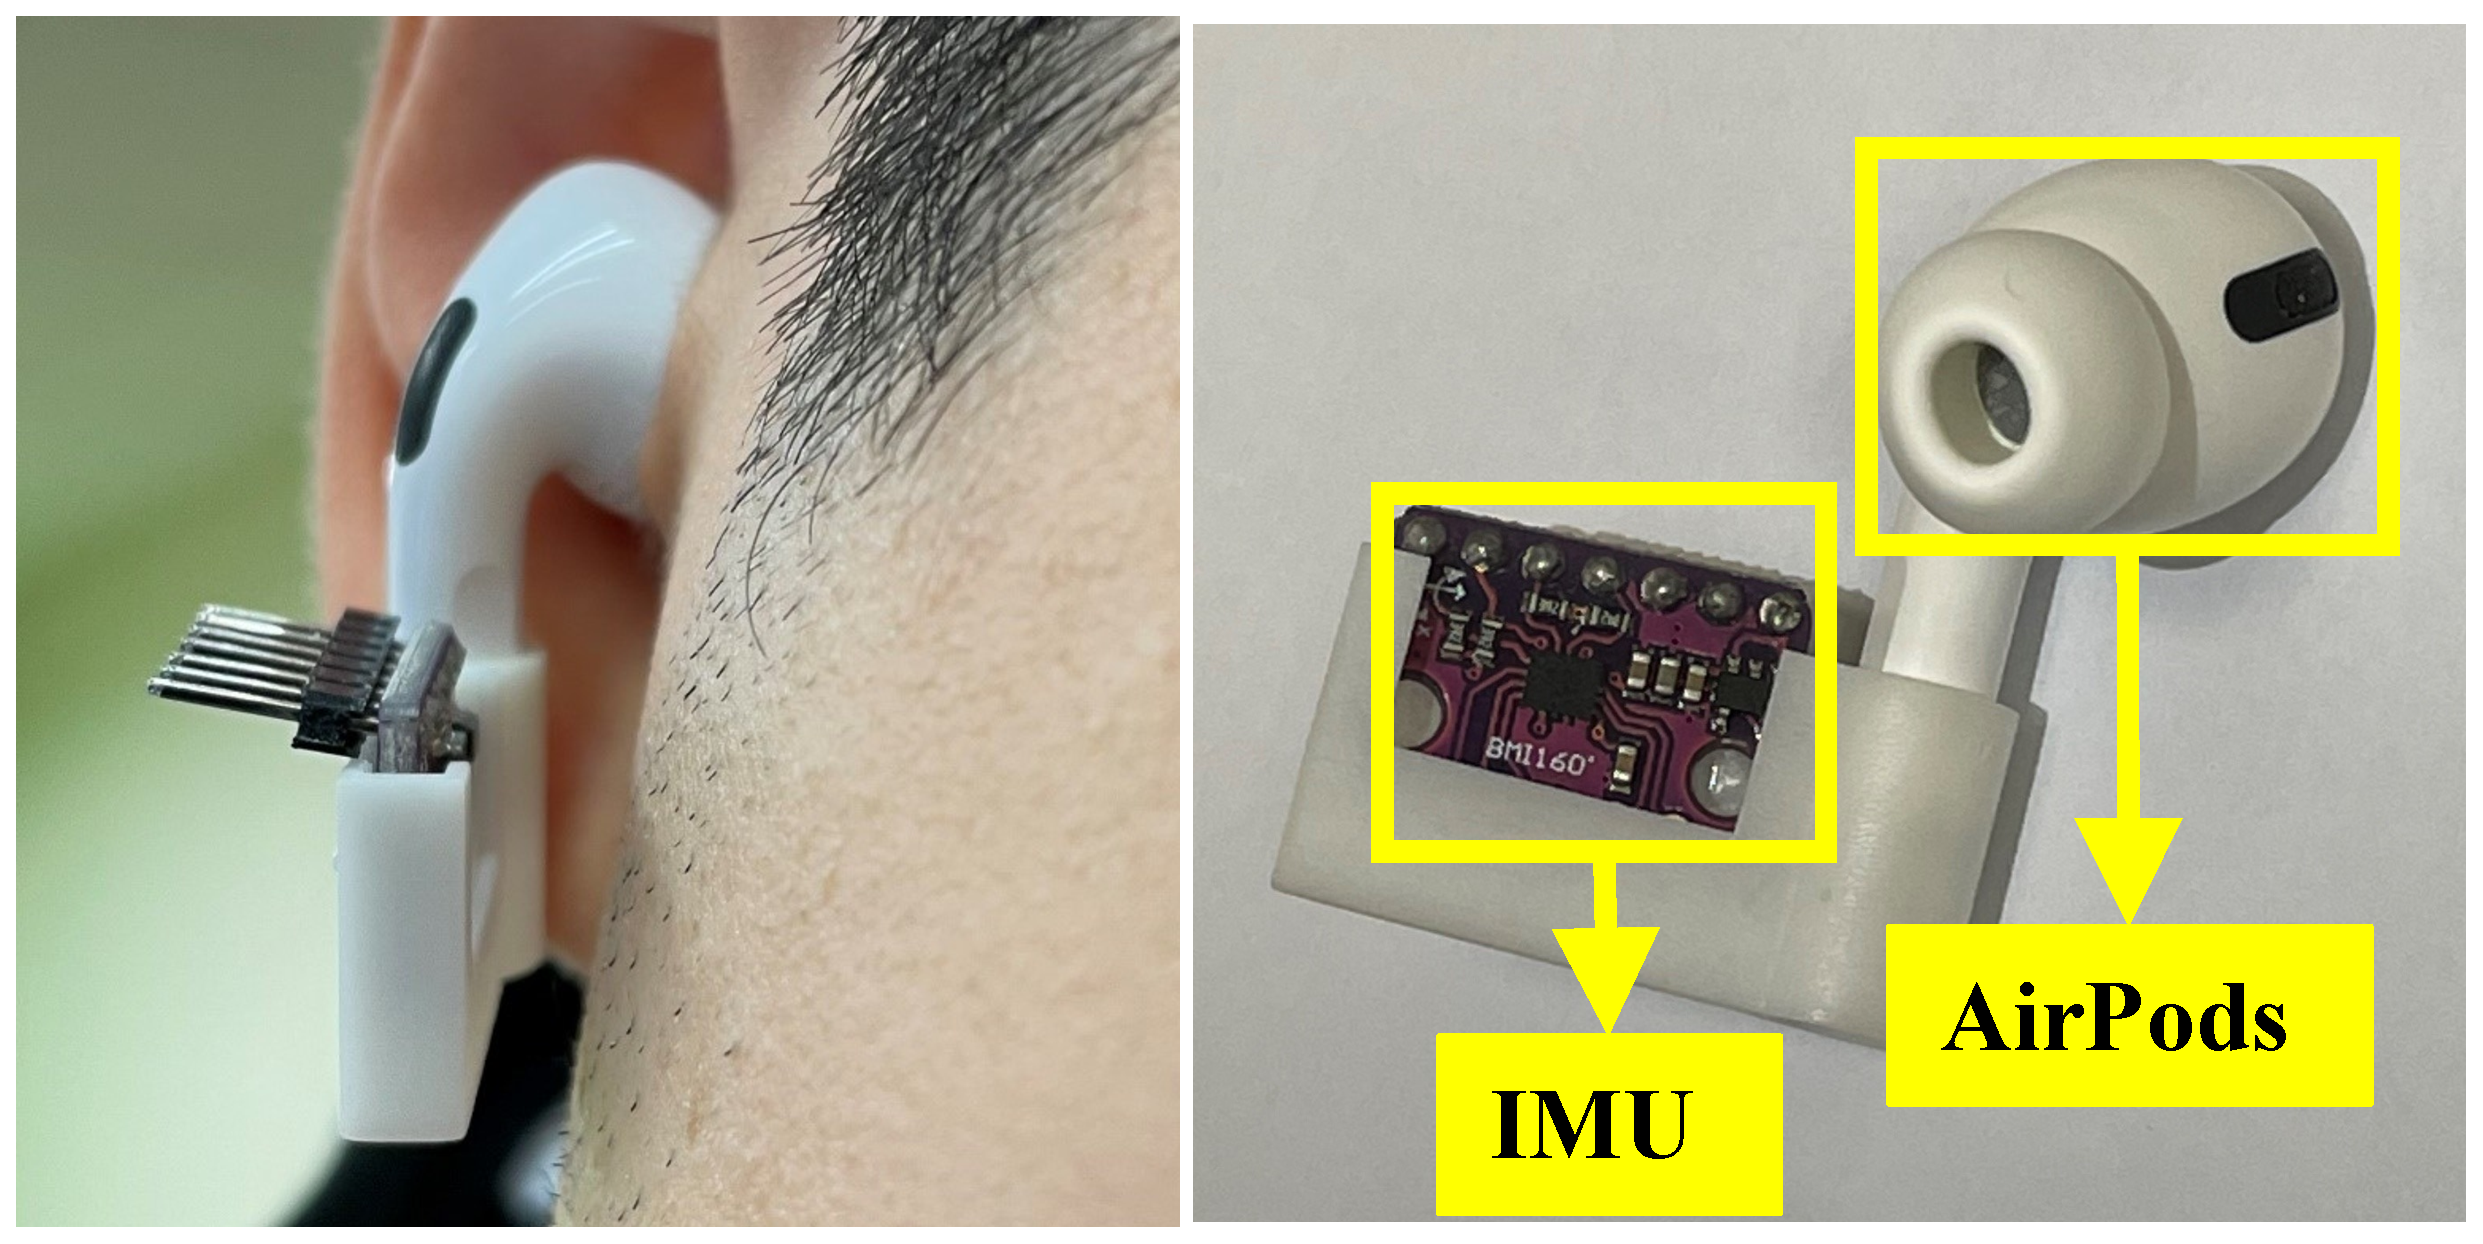
\includegraphics[width=\textwidth]{chapters/vibvoice/figure/earsense.eps}
    \caption{\emph{EarSense} with an Airpods Pro.}
    \label{fig:vibvoice_earsense-head}
  \end{subfigure}
  \begin{subfigure}{0.35\columnwidth}
    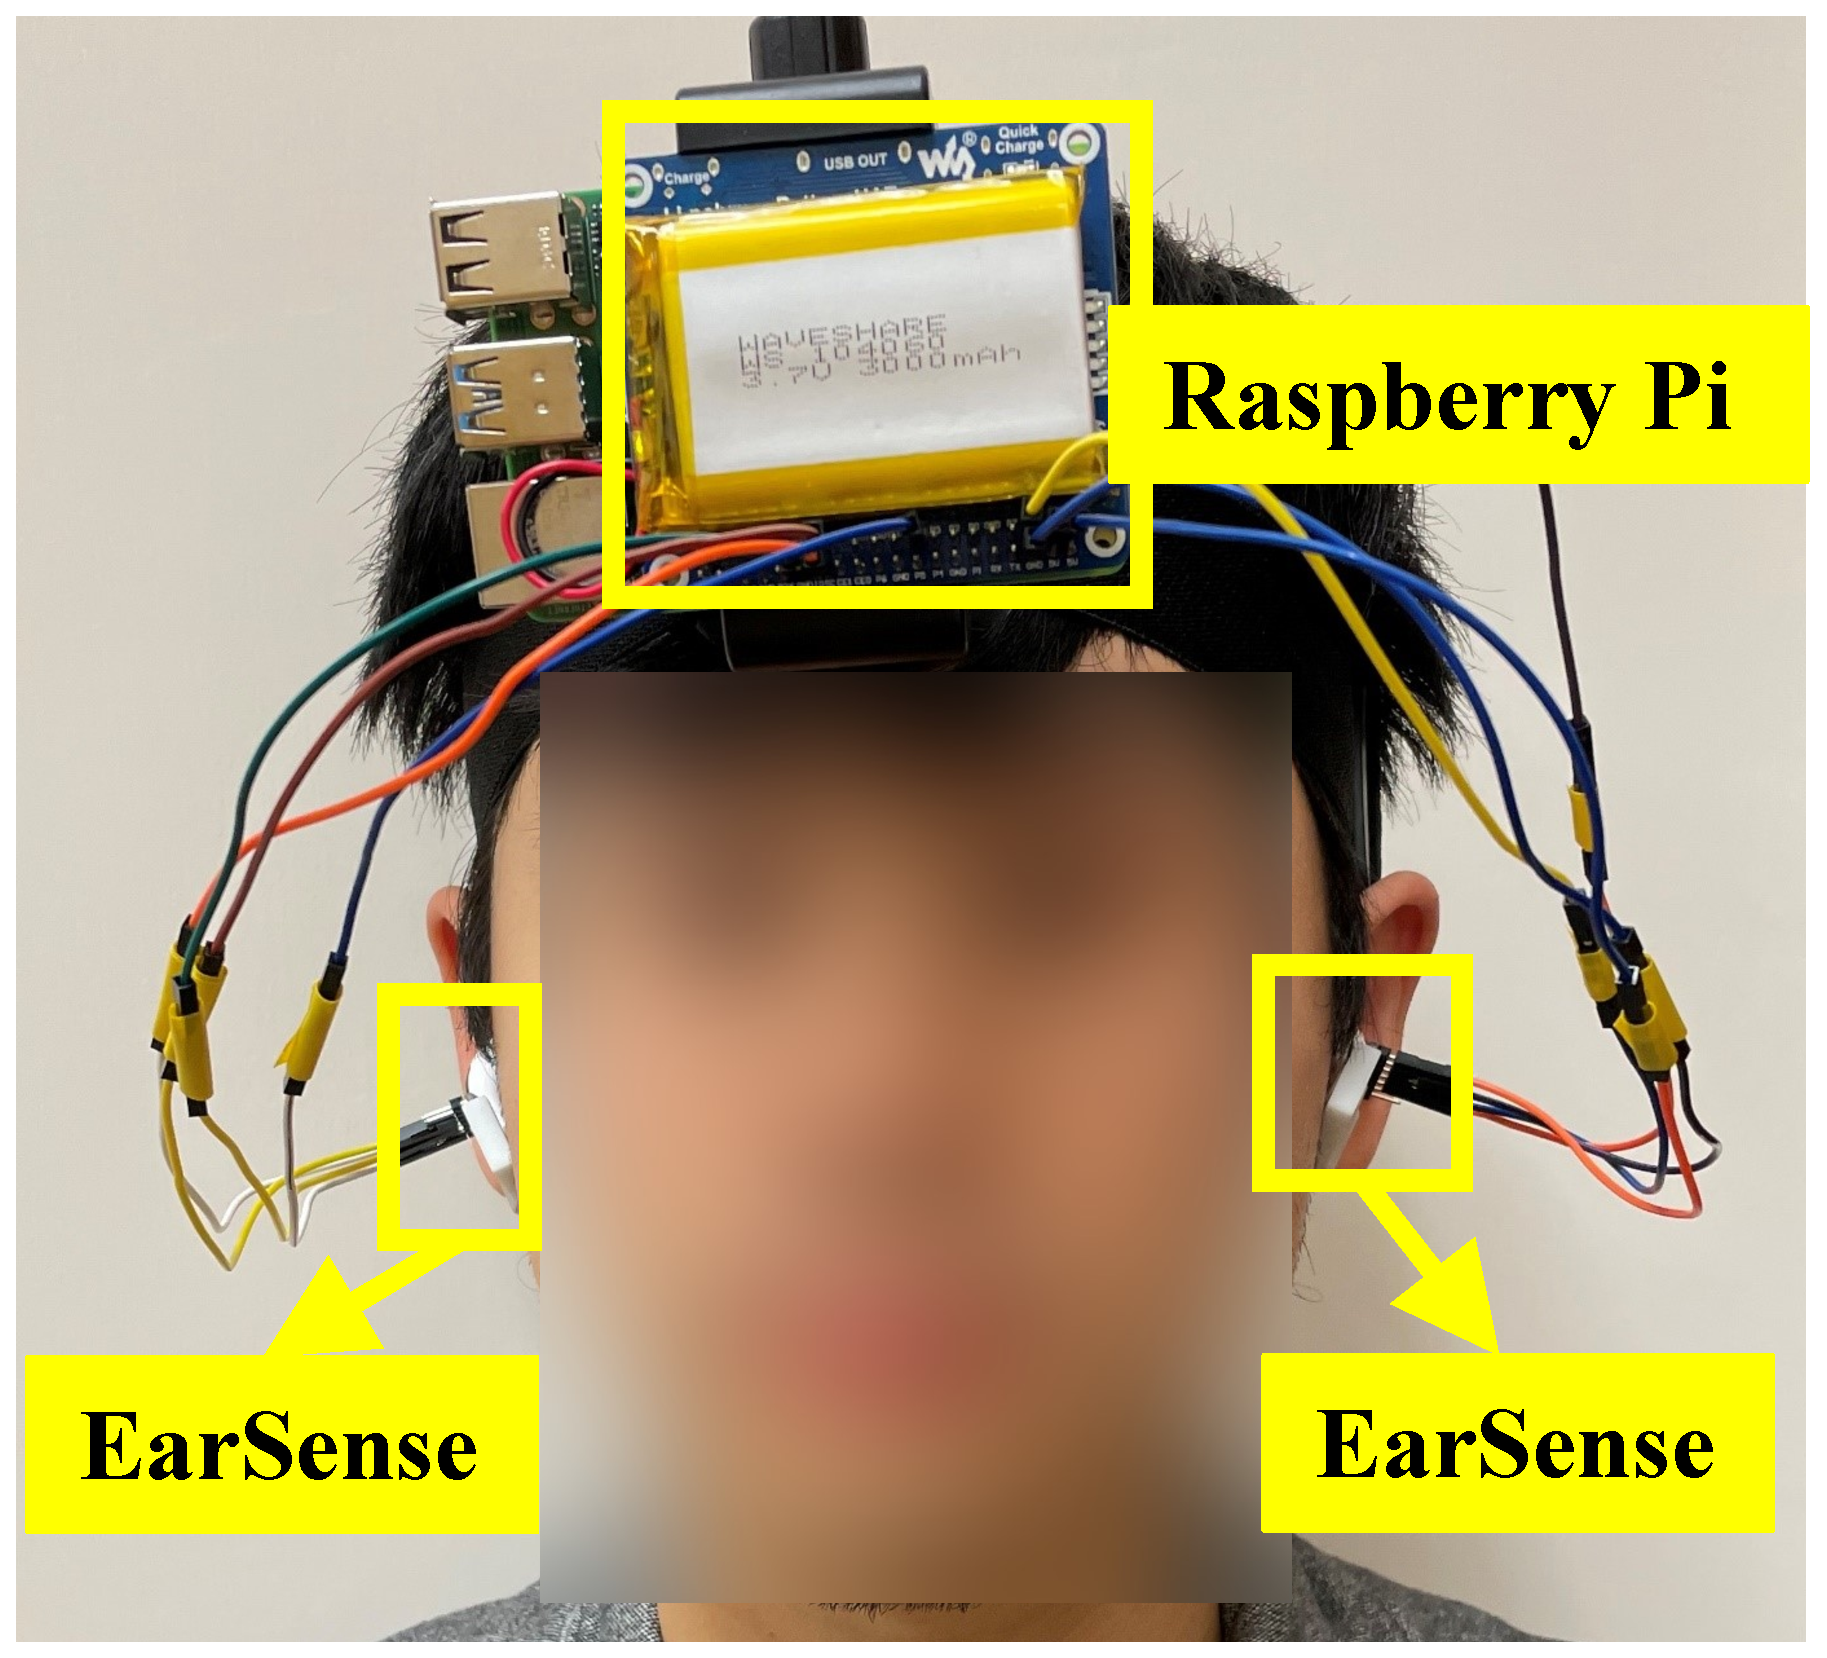
\includegraphics[width=\textwidth]{chapters/vibvoice/figure/people.eps}
    \caption{Test Setup.}
    \label{fig:vibvoice_earsense-people}
  \end{subfigure}
  \caption{\emph{EarSense} is an open-sourced data collector attachable to commercial HMWs for vibration sensing.}
  \label{fig:vibvoice_earsense}
\end{figure}

Fig. \ref{fig:vibvoice_earsense} shows the prototype of \textit{EarSense}  \citep{dataset}, a new open-sourced sensing platform that equips a 3D-printed enclosure with an IMU sensor (i.e., Bosch BMI-160 \citep{Inertial63:online}) inserted. EarSense has a flexible design to make it attachable to any commercial HMW device (e.g., AirPods Pro). EarSense captures the same vibration as the testing HMW and has no direct contact with the user's head (shown in Fig. \ref{fig:vibvoice_earsense-head}).
We connect two EarSenses to a Raspberry Pi (RPi) with a battery for data collection.
Fig. \ref{fig:vibvoice_earsense-people} shows a volunteer wearing the device on the head to avoid excessive vibrations caused by the connecting wires.
A Python script on the RPi controls the EarSense devices through the I2C protocol and stores the data for offline processing.
We only use the three-axis accelerometer provided by the IMU chip because the gyroscope and magnetometer are less related to the vibration.
The default sample rates of the microphone and accelerometer are $16\,\text{kHz}$ and $1.6\,\text{kHz}$, respectively. Since commercial earphones such as AirPods Pro do not support two-channel audio recording through public APIs, EarSense records audio in a mono channel.
We apply L2-Norm to the spectrograms of three-axis acceleration to extract the vibration intensity and avoid the impact of wearing position and user's motion.

\subsection{Measurements of Bone-Conducted Vibrations}
\label{sec:vibvoice_measurement}
We measure the difference between audio and bone-conducted vibrations with EarSense under various settings, i.e., the noises caused by the competing speaker and user motion. In each experiment, we ask a volunteer to wear Apple AirPods Pro with EarSense attached (shown in Fig. \ref{fig:vibvoice_earsense-people}) in a meeting room with the size of $10~\text{m}^2$. 
\begin{figure}
    \begin{subfigure}{0.46\columnwidth}
        \centering
        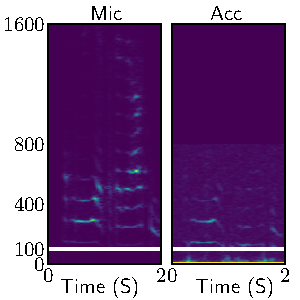
\includegraphics[width=1\textwidth]{chapters/vibvoice/figure/clean.pdf}
        \caption{The user is talking with no noise.}
        \label{fig:vibvoice_nospeaker}
        \end{subfigure}
        \hspace{.5em}
    \begin{subfigure}{0.46\columnwidth}
        \centering
        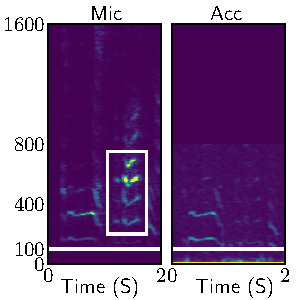
\includegraphics[width=1\textwidth]{chapters/vibvoice/figure/noise.pdf}
        \caption{The user is talking with a competing speaker.}
        \label{fig:vibvoice_speaker}
         \end{subfigure}
    \caption{Impact of the competing speaker.}
    \label{fig:vibvoice_competing-speaker}
\end{figure}

\noindent\textbf{Competing speaker.}
First, we ask the user to sit in the meeting room and speak while a loudspeaker is playing a pre-recording speech one meter from the user as the competing speaker. Note that the competing speaker is one of the most challenging environmental noises for HMWs since its spectrum is similar to the speech's, making it indistinguishable from the noise suppression algorithms. 
We set the volume of the competing speaker to be similar to the user, in which SNR is 3 dB. It is difficult to separate the two sources according to volume since the two speeches are mixed.
Fig. \ref{fig:vibvoice_nospeaker} and Fig. \ref{fig:vibvoice_speaker} show the spectrograms of microphone audio and acceleration when the environment is quiet or contains a competing speaker when the user is talking, respectively.
Note that we only show the spectrogram up to $1.6\,\text{kHz}$ since there is slim energy in the frequency bands higher than $1.6\,\text{kHz}$ of the microphone, and the accelerometer can only sense the signal with a frequency band of $800\,\text{Hz}$.
The spectrograms show that acceleration has lower signal energy than microphone audio since acoustic vibration attenuates during bone conduction, especially for high-frequency vibrations. Compared with the silent environment, the audio spectrogram of microphone audio with a competing speaker shows strong distortions, as highlighted with the white box in Fig. \ref{fig:vibvoice_speaker}. However, the accelerometer spectrograms do not show this phenomenon because the competing speaker cannot produce bone-conducted vibrations.
In summary, the accelerometer receives the user's voice through bone conduction only, excluding environmental sounds over the air, which is ideal for speech enhancement.

\noindent\textbf{User motion.}
We also measure the noises caused by the user's motion. We ask the volunteer to walk while talking. Fig. \ref{fig:vibvoice_walk} shows that walking causes low-frequency noises in the acceleration. The green boxes show the zoom-in result of the signals below $100\,\text{Hz}$. We can observe clear periodic fluctuations in low frequency (i.e., $< 50\,\text{Hz}$), which are caused by the steps of the volunteer.
In summary, the user's motion only affects the acceleration at lower frequencies, which does not affect our speech enhancement.
In addition, we observe slight low-frequency fluctuation in acceleration in Fig. \ref{fig:vibvoice_competing-speaker}, although the volunteer is asked to stand still in this experiment. Since most of the human speech is above $85~\text{Hz}$ \citep{Voicefre75:online}, the removal of audio in low frequency (i.e., the white horizontal lines in Fig. \ref{fig:vibvoice_competing-speaker}) can effectively reduce the interference caused by human motion.

\begin{figure}
\begin{minipage}[t]{0.46\columnwidth}
     \centering
        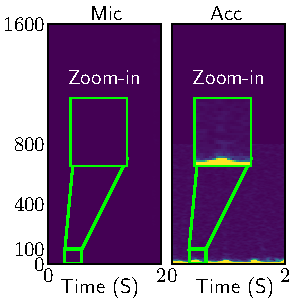
\includegraphics[width=1\textwidth]{chapters/vibvoice/figure/notalk.pdf}
        \caption{Spectrograms of microphone and acceleration when the user is walking.}
        \label{fig:vibvoice_walk}
\end{minipage}
\hfill
   \begin{minipage}[t]{0.48\columnwidth}
     \centering
       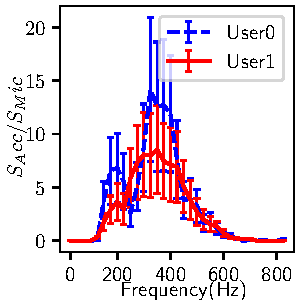
\includegraphics[width=1\textwidth]{chapters/vibvoice/figure/transfer_variance.pdf}
    \caption{Frequency responses of two users' bone-conducted vibrations.}
    %\vspace{-2em}
    \label{fig:vibvoice_bcf}
\end{minipage}
\end{figure}

\noindent\textbf{Frequency Response.}
We further explore the frequency response of bone-conducted vibrations among users. 
Specifically, we measure the frequency response of bone-conducted vibrations as follows: First, we compute the spectrums of audio and vibration data, which is denoted by $S_{Mic}$ and $S_{Acc}$, respectively. Then, we compute the Bone Conduction Function denoted by the frequency response of bone-conducted vibrations by $S_{Acc}/S_{Mic}$ at every frequency band. Fig. \ref{fig:vibvoice_bcf} shows two volunteers' frequency responses, in which the error bars represent the averages and variances.
The acceleration shows higher sensitivity than the microphone within the frequency of $200\text{Hz}\sim500\text{Hz}$, while lower sensitivity at a higher frequency ($>500\text{Hz}$) due to the absorption by the head skull. 
In addition, the frequency response keeps significant similarity among users, indicating the generalization to other users.
Hence, the Bone Conduction Function should consider inter-people diversity and inter-people similarity.

\begin{figure}
\begin{minipage}[t]{0.48\columnwidth}
     \centering
    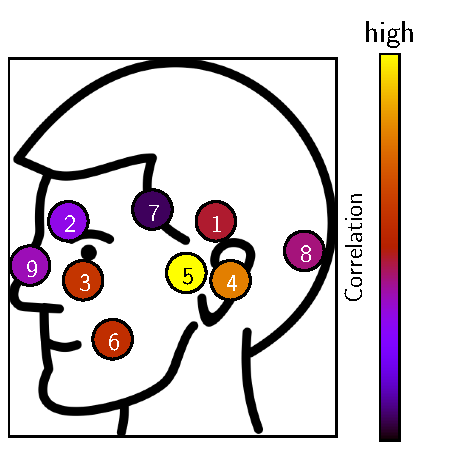
\includegraphics[width=\textwidth]{chapters/vibvoice/figure/correlation.pdf}
    \caption{Intensities of received bone-conducted vibrations on ten locations of the head.}
    \label{fig:vibvoice_head_positison}
\end{minipage}
\hfill
   \begin{minipage}[t]{0.48\columnwidth}
     \centering
    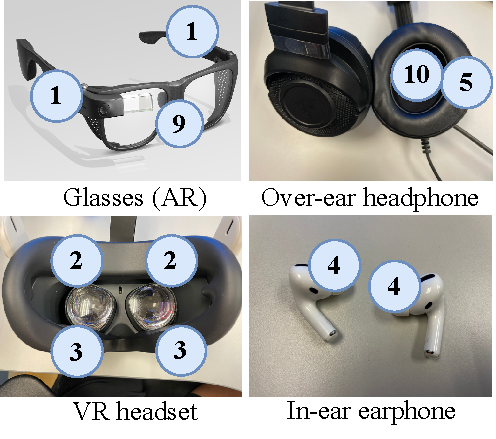
\includegraphics[width=\textwidth]{chapters/vibvoice/figure/devices.pdf}
    \caption{Potential placements on devices.}
    \label{fig:vibvoice_devices}
\end{minipage}
\end{figure}
\noindent\textbf{Locations on the head.}
Bone-conducted vibration exists at various locations on the head. 
As shown in Fig. \ref{fig:vibvoice_head_positison}, we select ten unique locations of interest on the head and measure the intensities of received bone-conducted vibrations. In particular, the nine locations are \#1 \emph{upper ear}, \#2 \emph{eyebrow}, \#3 \emph{cheekbones}, \#4 \emph{ear}, \#5 \emph{temporomandibular joint}, \#6 \emph{cheek}, \#7 \emph{temple}, \#8 \emph{back of the head}, and \#9 \emph{nose}. In addition, we tape EarSense on the interior of the pad of an over-ear headphone, which is denoted as \#10.
Among those positions, some are compatible with commercial HMWs like glasses, headphones, and VR headsets. Fig. \ref{fig:vibvoice_devices} illustrates the corresponding positions on HMWs. The numbers on the HMWs correspond to the locations in Fig. \ref{fig:vibvoice_head_positison}. 
We attach EarSense to the HMWs (when applicable) or on the face for all the following tests. 
We compute Pearson correlation coefficients between the audio and the acceleration on each location and mark the values using a color map in Fig. \ref{fig:vibvoice_head_positison}.
We observe that bone-conducted vibrations exist at most locations of the head. In particular, locations closer to the mouth show higher correlations, indicating a larger possibility of extracting clean speech. 

In summary, our measurements show that bone-conducted vibration has the following characteristics: a) Bone-conducted vibration is robust to environmental voice and only captures the user's speech; b) The user's motion only generates vibrations lower than $85\,\text{Hz}$; c) Bone-conducted vibration has suppressed low and high-frequency audio, which varies across users and within the same user; and d) We can receive audio from multiple locations on the head.


% \section{Motivation Study}
\label{sec:egolog_measurement}
As discussed in Sec. \ref{sec:egolog_intro}, we mainly have three challenges towards a multi-modal HAR on mobile devices: 1) lack of scenario awareness, 2) being sensitive to ambient noise, and 3) fusion collapse. To explore these challenges and evaluate the potential for overcoming them, we conduct a series of experiments to analyze and demonstrate promising directions.

\begin{figure}
    \centering
    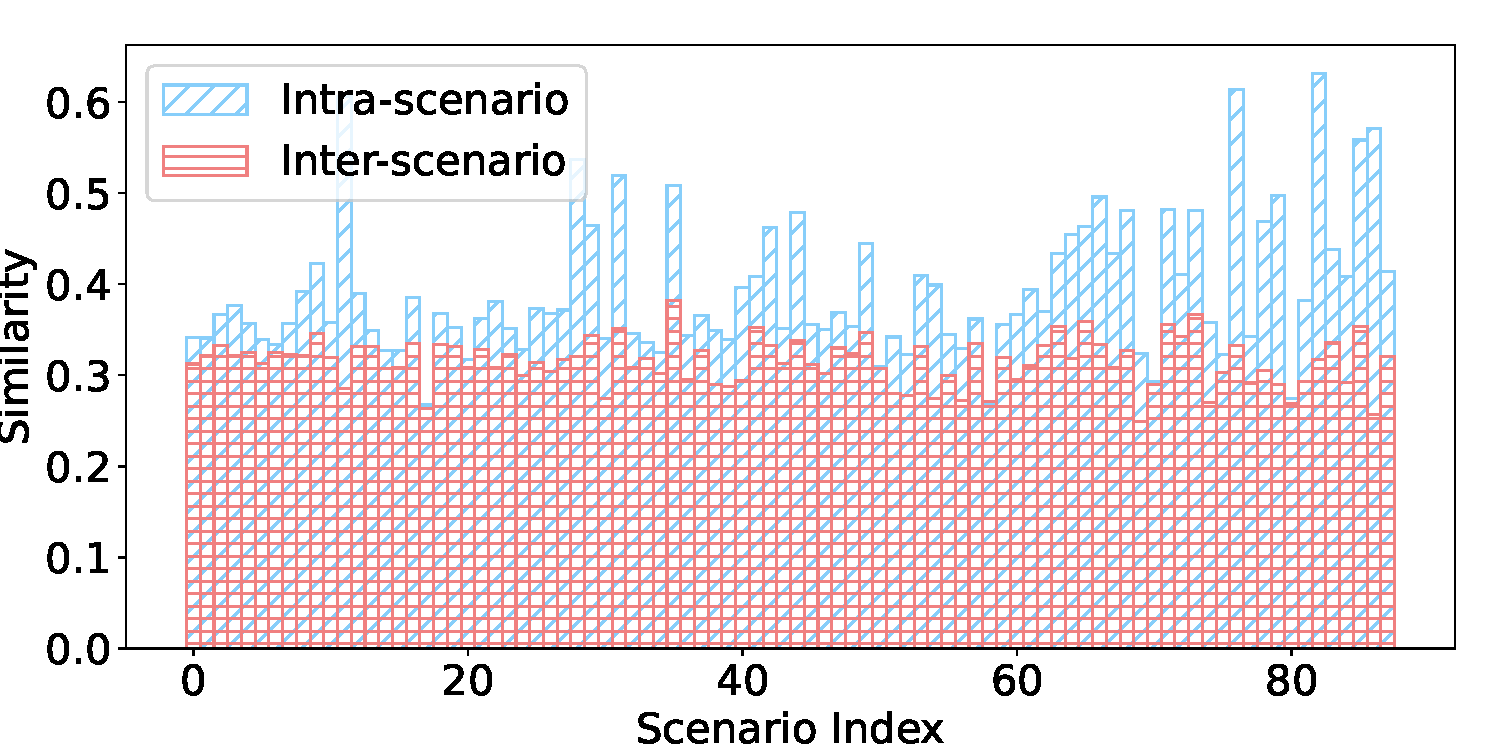
\includegraphics[width=0.8\linewidth]{chapters/egolog/figs/scenario_similarity.pdf}
    \vspace{-1em}
    \caption{Motivation for scenario understanding: 
    The similarity of embeddings for intra- and inter-scenario activities.}
    \label{fig:egolog_scenario_similarity}
    \vspace{-1em}
\end{figure}

\subsection{Scenario}
\label{subsec:scenario}
Scenario information refers to long-time activities (e.g., playing with a pet or working at home) that reflect the user's real-world behavior. Capturing such scenarios in datasets is challenging, as it requires volunteers to perform activities naturally, mimicking real-life conditions. Generally, scenario is the ensemble of multiple related and continuous activities with a realistic distribution, reflecting meaningful interactions with the environment.

To investigate the impact of scenario information on HAR, we use the Ego4D dataset~\citep{grauman2022ego4d}, which captures real-world activities through smart glasses equipped with IMU and audio sensors. The dataset provides annotations at both the window level (every 10 seconds) and the video level, represented as plain text. We treat window-level annotations as activity labels and video-level annotations as scenario labels that describe the broader setting of prolonged activities. To examine scenario properties, we use Sentence-BERT~\citep{reimers2019sentence} to generate text embeddings for activities across 91 scenarios. We then compute activity similarity both within scenarios (intra-scenario) and between scenarios (inter-scenario). Intra-scenario similarity measures the similarity of activities within the same scenario, while inter-scenario similarity compares an activity from one scenario to a randomly selected activity from a different scenario.

The results are shown in Fig.~\ref{fig:egolog_scenario_similarity}, revealing that the similarity within a scenario (intra-scenario similarity) is over 20\% higher than the similarity between different scenarios (inter-scenario similarity). This suggests that each scenario has a distinct distribution of activities. Specifically, a scenario effectively represents the user's daily log since it encompasses a longer time frame.
Additionally, we notice that the inter-scenario similarity is generally above 0.3, indicating that many basic activities (such as sitting and walking) are common across all scenarios. Therefore, it is crucial to eliminate the influence of these basic activities in scenario recognition, as they are present in every scenario.


In summary, the in-the-wild dataset shows that scenarios have distinct activity distributions, which can support scenario recognition through scenario-specific activities.


\subsection{Sound Location }
\label{subsec:embodied}
\begin{figure}
    \centering
    \begin{minipage}{0.48\linewidth}
        \centering
       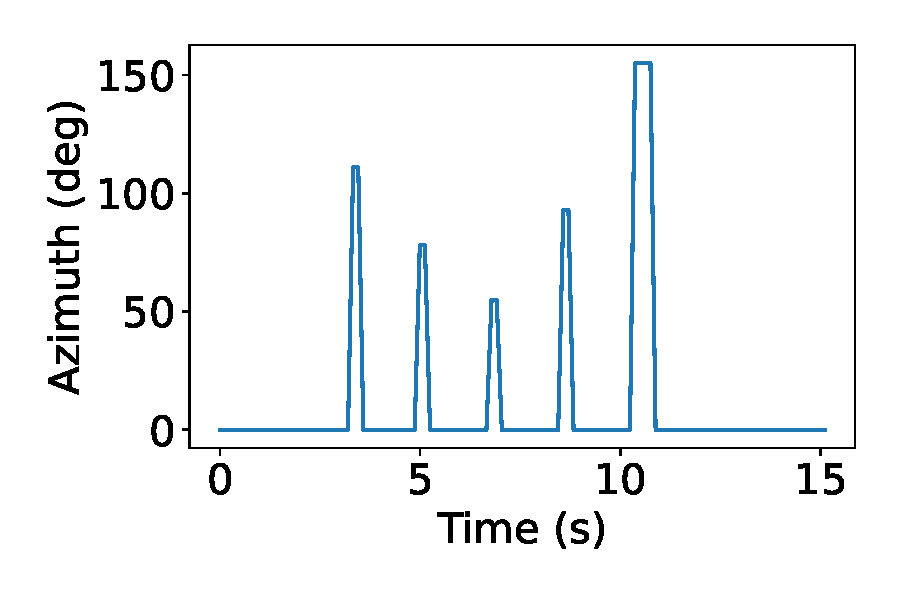
\includegraphics[width=\linewidth]{chapters/egolog/figs/baseline_result.pdf}
        \caption{Sound localization \citep{schmidt1986multiple} under motion}
        \label{fig:egolog_loc_move}
    \end{minipage}
    \hfill
    \begin{minipage}{0.48\linewidth}
        \centering
        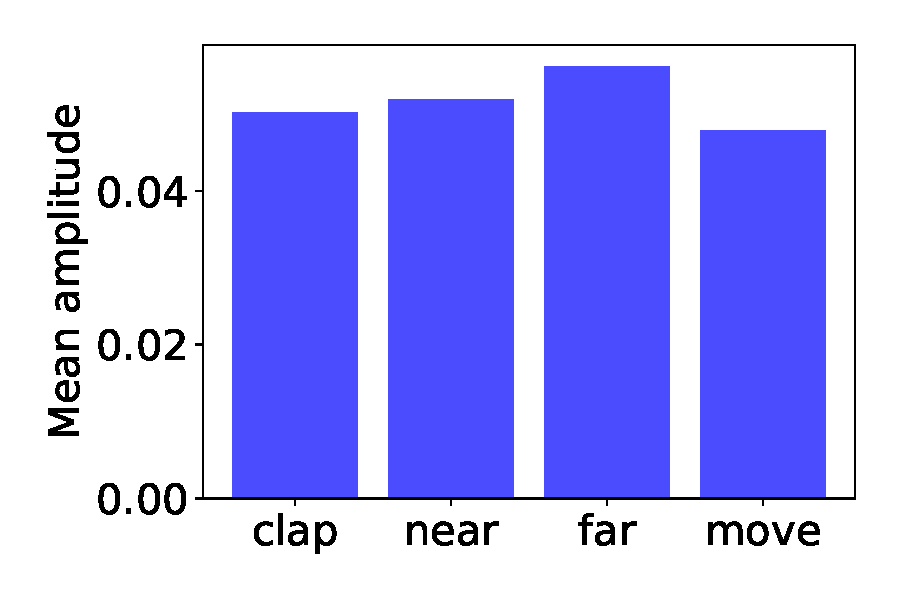
\includegraphics[width=\linewidth]{chapters/egolog/figs/amplitude.pdf}
        \caption{Sound volume may not related to distance.}
        \label{fig:egolog_amplitude}
    \end{minipage}    
    \vspace{-1em}
\end{figure}

\begin{figure}
    \centering
    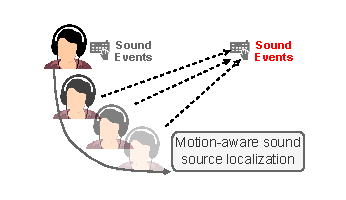
\includegraphics[width=0.75\linewidth]{chapters/egolog/figs/spatial_motivation.pdf}
    \vspace{-1em}
    \caption{Motivation for spatial understanding: estimate the distance of a sound event by motion.}
    \vspace{-1em}
    \label{fig:egolog_motivation_localization}
\end{figure}

In practice, recorded audio often includes far-field sound sources that are unrelated to the user’s activities, underscoring the importance of sound localization for effective HAR. Wearables that are consistently worn on the user’s head provide a stable and reliable position for capturing detailed ambient sound information. Additionally, modern wearables feature multi-channel recording capabilities, enhancing their spatial sensing potential.
In the following, we divide sound localization into direction and distance estimation, which we discuss as follows.

The estimation of sound direction is one of the mature, basic, but still challenging applications of a microphone array. The accuracy highly depends on the number of microphones, which is unfortunately not sufficient for most commercial devices. Considering the most common setting of stereo recording, there are mainly two problems: the deviation of direction (especially for front-back confusion) and estimation of sound distance, as illustrated in Fig. \ref{fig:egolog_motivation_localization}.
We envision that the above challenges may be solved by motion compensation. Specifically, we can aggregate the consecutive sound localization results along with the movement of the user (microphone) to refine the results or even get the distance.

To illustrate these challenges, we positioned a sound source in front of the user and used a binaural microphone with the algorithm from~\citep{schmidt1986multiple} to estimate direction of arrival, as shown in Fig.~\ref{fig:egolog_loc_move}. The user was instructed to move the body slightly and naturally. The estimate fluctuated around the true value of 90 degrees. To test whether sound volume is sufficient for differentiating near and far sources, we conducted an experiment with the sound source at different distances from the microphone. As shown in Fig.~\ref{fig:egolog_amplitude}, volume differences were not reliable across distances. The final bar in Fig.~\ref{fig:egolog_amplitude} also shows that user movement slightly affects amplitude. Multiple sound sources can further complicate volume-based distance estimation.

\subsection{Multi-modal Fusion }
\label{subsec:measure-fuse}

\begin{figure}
    \centering
     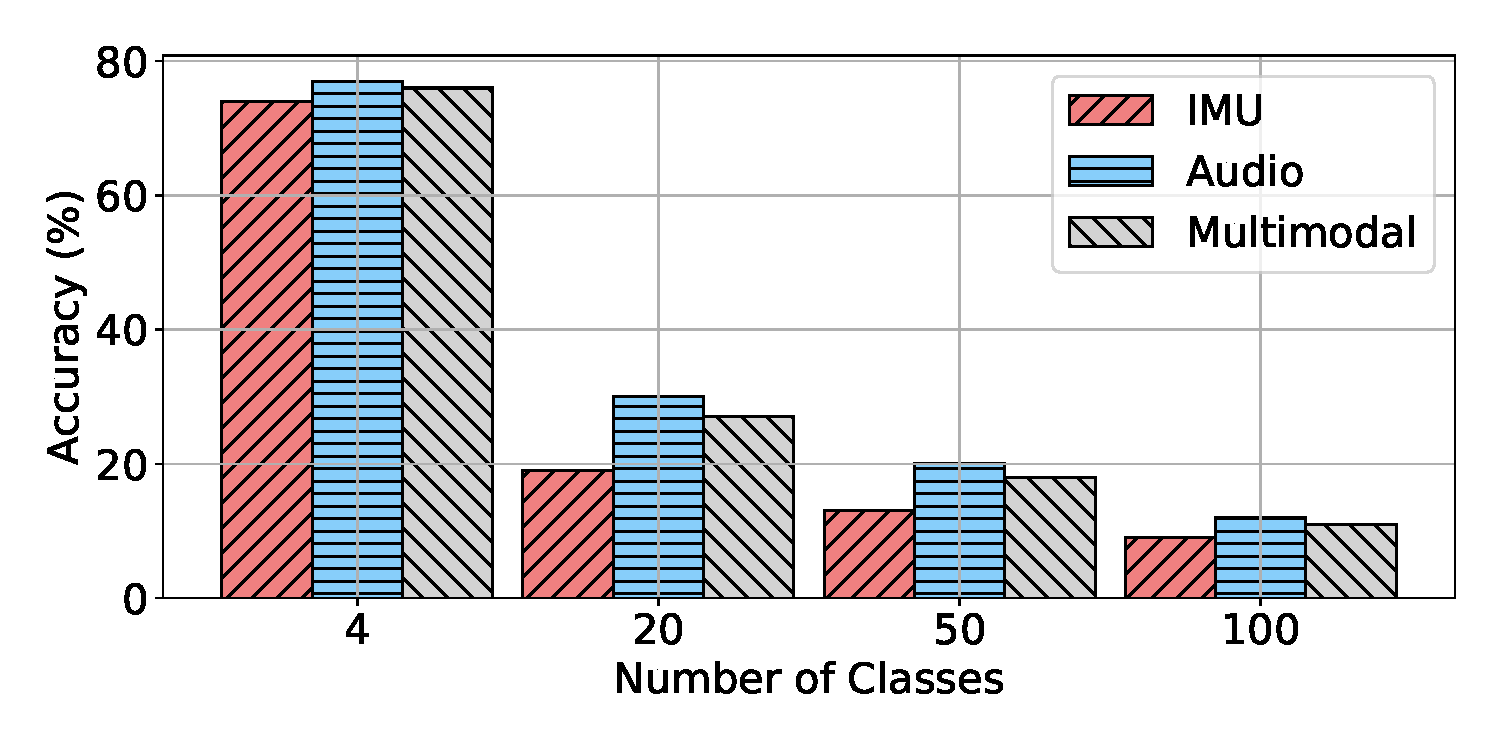
\includegraphics[width=.75\linewidth]{chapters/egolog/figs/num_class.pdf}
     \vspace{-1em}
      \caption{The performance of an existing activity recognition with different class numbers and modalities.}
    \label{fig:egolog_num_class}
    \vspace{-1em}
\end{figure}

To investigate scalability bottlenecks in activity recognition using wearables, we trained unimodal supervised models with audio and IMU data on the Ego4D episodic memory subset (200 activity classes). We used EfficientAT~\citep{schmid2023efficient} for audio and LIMU-BERT~\citep{xu2021limu} for IMU as feature extraction backbones, comparing them to a multi-modal model via late fusion. Activities were clustered into varying class numbers using Sentence BERT~\citep{reimers2019sentence} embeddings and K-Means~\citep{macqueen1967some}, following MMG-Ego4D~\citep{gong2023mmg}. Results (Fig.~\ref{fig:egolog_num_class}) show a significant performance drop as class numbers increase, indicating challenges in recognizing diverse activities with audio or IMU alone. Multimodal fusion often underperforms unimodal models, suggesting ineffective extraction of complementary features at larger scales.

\begin{figure}
    \centering
    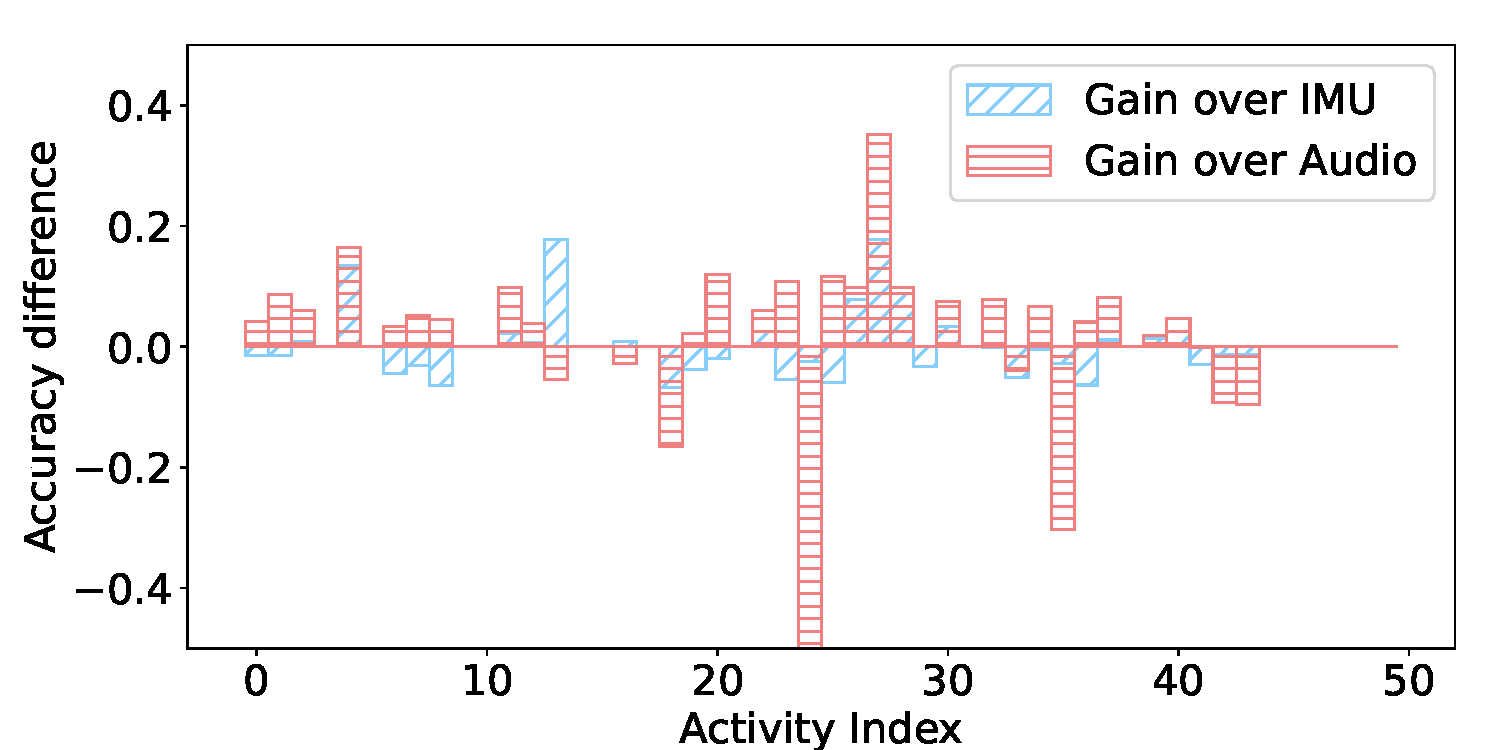
\includegraphics[width=.75\linewidth]{chapters/egolog/figs/activity_diff.pdf}
    \vspace{-1em}
    \caption{Performance gain from multi-modal fusion.}
    \label{fig:egolog_acc_gap}
    \vspace{-1em}
\end{figure}

Previous work~\citep{mollyn2022samosa} demonstrates that multi-modal learning can outperform the unimodal model due to the complementary nature of each other.
However, this finding does not apply to all cases. Another study~\citep{gong2023mmg} finds that multimodal learning with audio and IMU on Ego4D can perform worse than single-modality solutions. To investigate this result, we compared the accuracy of multimodal and unimodal models for each class, as shown in Fig.~\ref{fig:egolog_acc_gap}. The benefits of multimodal fusion fluctuate across both modalities, indicating that supervised multimodal learning cannot automatically select the appropriate modality for each activity.


To investigate whether LLMs can alleviate this problem, we evaluate ImageBind-LLM~\citep{han2023imagebind}, which converts both modalities into features and prepends them to text embeddings. We instruct the model with the prompt: ``<sensor> According to the audio and IMU reading on the earphone of the user, what is the activity of the user?'', where <sensor> denotes the inserted sensor features. Since LLM outputs can be random, we also constrain the prompt to one of the candidate activities. To reduce complexity, we select the top 30 activities from the Ego4D episodic memory subset. ImageBind-LLM achieves BERT-score precision, recall, and F1 score of 0.04, 0.07, and 0.05, respectively. Because this performance is low, we inspect the outputs and find that the LLM may not fully understand the multimodal fusion task.
We further test whether fine-tuning can address this problem by training an adapter~\citep{zhang2023llamaadapter} for ImageBind-LLM. The adapted LLM achieves BERT-score precision, recall, and F1 score of 0.47, 0.46, and 0.47, respectively. Although fine-tuning improves performance, the result remains below the level needed for practical use.

% \section{Background}
\label{sec:cohear_background}

This section lays the technical foundation for CoHear, focusing on acoustic sensing techniques used for conversation modeling.
First, it discusses sound localization, which estimates speaker positions from earphone microphone arrays and provides information for constructing a conversation map.
It then reviews wireless acoustic sensor networks (WASNs), which support collaborative sensing across multiple devices.


\subsection{Sound Source Localization}
Sound source localization is a core problem in multi-channel audio and enables spatial acoustic sensing.
Consider a microphone array consisting of $N$ microphones located at known positions $\mathbf{p}_i = (x_i, y_i)$ for $i = 1, 2, \ldots, N$. Let the position of the sound source be denoted by $\mathbf{s} = (x_s, y_s)$.
The time it takes for the sound to reach the microphone $i$ can be expressed as:
\(t_{s, i} = \frac{d_{s, i}}{c}, d_{s, i} = \sqrt{(x_s - x_i)^2 + (y_s - y_i)^2}\)
where $d_{s, i}$ is the distance from sound source $s$ to microphone $i$, and $c$ is the speed of sound in air. Since the source emission time is unknown to the receiver, $t_{s, i}$ cannot be estimated directly. Instead, the system estimates the time difference of arrival (TDoA), $t_{s, i} - t_{s, j}$, where $i, j \in (1, N)$. A common method for estimating TDoA from in-the-wild recordings is the generalized cross-correlation (GCC)~\cite{knapp1976generalized}, which is computed for each microphone pair. The GCC peak estimates the TDoA, which can then be used to calculate the direction of arrival (DoA) as \(DoA = arctan((x_s - x_c)/(y_s - y_c))\), where $x_c$ is the center of the microphone array. This analysis shows why localization performance depends strongly on the number of microphones: more microphones provide more microphone pairs and therefore more TDoA constraints.

Instead of relying on analytical methods, sound source localization can be performed using a deep neural network, as explored in \cite{wang2022nerc}. This deep learning-based approach generally consists of two stages: feature extraction and location estimation.
In the feature extraction stage, the audio signal is typically converted into a spectrogram representation with dimensions: \(C\times T \times F\), where \(C\) refers to channels, \(T\) refers to time, and \(F\) refers to frequency. These features can be further processed using techniques such as log-melspectrogram conversion, which is applied to each channel individually, or multi-channel methods like GCC \cite{knapp1976generalized} and SALSA-Lite \cite{nguyen2022salsa}.
In the location estimation stage, the neural network is trained to output the sound source location, which also supports a dynamic number of simultaneous sound sources. For instance, architectures employing multi-track \cite{cao2021improved} or multi-ACCDOA \cite{shimada2022multi} output formats are designed specifically to localize overlapping sound events.

Deep sound localization can also use the spatial information embedded in binaural recordings, including reflections from the human head and body. Specifically, the head-related transfer function (HRTF) can be modeled as:
\(H_{L}(\theta, \phi, f, d) = \frac{Y_{L}(f)}{X(f)}, H_{R}(\theta, \phi, f, d) = \frac{Y_{R}(f)}{X(f)},\) where $H_{L}$ indicates the frequency response for left ear and $H_{R}$ indicates the frequency response for right ear. 
By using HRTF cues with deep learning, binaural localization can achieve higher accuracy than a linear two-microphone array. For instance, this approach can partially resolve front--back confusion, a problem that is particularly challenging for conventional two-microphone arrays.


\subsection{Wireless Acoustic Sensor Network}
We are studying a wireless acoustic sensor network where a group of sensor nodes is randomly distributed in a reverberant environment \cite{bertrand2011applications}. We assume that the internal geometric configuration of each node's microphone array is known and that all microphones within the array are sampled at the same time, which we believe is a reasonable assumption following \cite{gburrek2021geometry}. Additionally, we assume that there is coarse time synchronization among the clocks of the sensor nodes, enabling us to aggregate the data globally. By default, we assume a two-dimensional space, but it can be easily extended to a three-dimensional space.

Since a sensor node cannot determine its own position or orientation within the global coordinate system, all observations are made in the local coordinate system of each node. 
Each sensor node \( l \) (where \( l = 1, \ldots, L \)) computes acoustic features (e.g., DoA estimates \( \phi_k^l \) and distance \( d_k^l \)) to the acoustic source \( k \), all reference to the node's local coordinate system. Consequently, we gather a total of \( K \times L \) estimates as the inputs.

From the global view of the WASN, it is composed of \( L \) sensor nodes each equipped with a microphone array located at positions \( n_l = [n_{l,x}, n_{l,y}]^T \) and oriented at angles \( \theta_l \) (where \( l = 1, 2, \ldots, L \)) relative to a global coordinate system defined by the x and y axes. There are \( K \) acoustic sources located at positions \( s_k = [s_{k,x}, s_{k,y}]^T \) (where \( k = 1, 2, \ldots, K \)). Note that all the above global notations are unknown and will be estimated through a geometry calibration process based on the observed acoustic signals from sensor nodes.





This chapter outlines the principles of user–environment sensing using head-mounted wearables, focusing on topics within the scope of this thesis.
We first discuss the available sensing modalities, their properties, and limitations.
We then introduce the core algorithms that enable sensing with these modalities.
Lastly, we present measurement studies that substantiate and elaborate on the above discussions.

\section{Sensors on Head-mounted Wearables}
Modern head-mounted wearables are typically equipped with multiple sensors to capture various aspects of the user's environment and activities, including, but not limited to, microphones that capture audio, inertial measurement units (IMUs) that capture motion and orientation, and cameras that capture visual information. We discuss these in the following subsections.

\subsection{Microphone}
A microphone (mic) converts fluctuations in air pressure into an electrical signal. It is fundamental to telecommunication, audio capture, broadcasting, and many consumer devices, including phones, hearing aids, and head-mounted wearables. Common transduction mechanisms include dynamic moving-coil elements operating in a magnetic field, condenser (capacitor) capsules where a tensioned diaphragm forms one plate, and contact/piezo designs that exploit piezoelectric crystals. Because microphone outputs are low level, they are typically routed through a preamplifier before recording or playback.

Due to the compact form factor of head-mounted wearables, the microphones used in these devices are typically small and lightweight, which generally implies fewer microphones, a narrower frequency response, and lower sensitivity compared to professional-grade equipment.
Importantly, they are often omnidirectional, which offers broad applicability but also captures more ambient noise.

In head-mounted wearables, microphones are the primary means of capturing the user's voice and ambient sound.

\subsection{Inertial Measurement Unit}
Inertial Measurement Units (IMUs) are electronic devices that measure and report a body's specific force, angular rate, and sometimes the magnetic field surrounding the body, using a combination of accelerometers, gyroscopes, and optionally magnetometers. The traditional application of IMUs is tracking the orientation and movement of objects, such as in aerospace, robotics, and consumer electronics like wearables.

Combining IMUs with other sensors, such as cameras or Global Positioning System (GPS), provides more accurate and robust motion tracking and navigation capabilities, addressing challenges such as error accumulation in IMU-only systems.

IMUs are now used beyond tracking. In particular, they are key sensors for activity recognition by analyzing complex patterns in the IMU readings. IMUs are ubiquitous, low-power, and privacy-preserving—key advantages over many other sensors. Major applications include step counting, gait analysis, sports recognition, gesture recognition, and fall detection.

\subsection{Cameras}
Cameras are optical devices that capture visual information by recording light patterns onto a photosensitive surface or digital sensor. They are widely available on head-mounted wearables, especially high-end devices like AR/VR headsets and smart glasses. 

The applications of cameras on head-mounted wearables are diverse, ranging from recognizing the user (e.g., expression, eye movement, hand movement) to sensing the surrounding environment (e.g., object tracking).
Although cameras are powerful, they also bring significant challenges in terms of privacy, power consumption, and data processing requirements.
Within the scope of this thesis, we mainly focus on applications that do not assume cameras, making the methods applicable to more general head-mounted wearables. Integration of camera data can, of course, further enhance system performance.

\subsection{Speaker}
A speaker is an electroacoustic transducer that converts an electrical audio signal into corresponding sound—the reverse of a microphone.
Speakers are designed for audio output (communication, media playback, notifications), not sensing. However, researchers have discovered that speakers can also be used as sensors in certain scenarios. For example, by analyzing reflected sound waves emitted by a speaker, it is possible to infer information about the surrounding environment, such as distance to objects or movement patterns—similar to sonar or echolocation. This principle is applicable to head-mounted wearables with built-in speakers.

\subsection{Biometric Sensor}
Due to the proximity of head-mounted wearables to the skin and the head, they can also incorporate biometric sensors to monitor physiological signals. Common biometric sensors include photoplethysmography (PPG) sensors for heart rate monitoring, which can be embedded within earbud tips. Or, temperature sensors for skin temperature measurement. Except for the specific sensors of biometric, sensors like microphone and IMU can also be used for biometric purposes, e.g., using microphone for heartbeat detection via the ear-canal listening.

\section{Algorithms}
This section introduces the fundamental algorithms that enable user–environment sensing using the sensors on head-mounted wearables, within the scope of this thesis.

\subsection{Sound Enhancement and Separation}
Suppose the audio recorded by the microphone on head-mounted wearables is denoted as \(y(t)\), which is a mixture of the target sound \(s(t)\) and undesired noise \(n(t)\): \[y(t) = s(t) + n(t).\] A sound enhancement or separation algorithm aims to recover the target sound \(s(t)\) from the mixture \(y(t)\) by a model \(f(\cdot)\): \[\hat{s}(t) = f(y(t)),\] where \(\hat{s}(t)\) is the estimated target sound.

Notably, the "target" is scenario-dependent rather than fixed. For example, in speech enhancement the target is clean speech, whereas in music separation the target could be a specific instrument or vocal track. We therefore use the general term "sound enhancement and separation" to cover both tasks.

To achieve separation, one may use either traditional signal processing techniques or modern deep learning-based methods. Traditional techniques include spectral subtraction, Wiener filtering, and beamforming, which rely on statistical properties of noise so that the algorithm can filter out similar components: \[ \hat{s}(t) = f(y(t), n_{\text{ref}}(t)).\]
With the advancement of deep learning, data-driven approaches have become increasingly popular and often achieve superior performance.
Generally, deep learning models do not rely on explicit assumptions about noise characteristics; instead, they learn to distinguish target from noise using large datasets: \[ \hat{s}(t) = f_{\theta}(y(t)).\] Although large datasets confer strong generalization capability, models may still lack adaptability to unseen noise types and acoustic conditions.

Recently, target sound extraction has been proposed to further improve performance, where an additional reference signal \(s_{\mathrm{ref}}(t)\) is provided to guide the model to focus on the desired target: \[ \hat{s}(t) = f_{\theta}\big(y(t), E\big(s_{\mathrm{ref}}(t)\big)\big),\] where \(E\) is an encoder that extracts target characteristics from the reference signal (which can be any signal related to the target sound). This paradigm is a form of multi-modal learning, where the model leverages information from multiple modalities to enhance performance. 

\subsection{Multi-channel Audio Processing}
\label{sec:cohear_background}

This section lays the technical foundation for multi-channel audio processing, which is essential for the design in \ref{ch:cohear}. The basic assumption is that more than one microphone is available for audio recording, which differs from single-microphone processing.
First, we discuss sound localization, which identifies speaker positions using earphone microphone arrays, providing essential information to create a conversation map.
Next, we review Wireless Acoustic Sensor Networks (WASNs), which facilitate collaborative sensing across multiple devices.

\subsubsection{Sound Source Localization}
Sound source localization is one of the hot topics for multi-channel audio, which enables spatial sensing capability for audio.
Consider a microphone array consisting of $N$ microphones located at known positions $\mathbf{p}_i = (x_i, y_i)$ for $i = 1, 2, \ldots, N$. Let the position of the sound source be denoted by $\mathbf{s} = (x_s, y_s)$.
The time it takes for the sound to reach the microphone $i$ can be expressed as:
\(t_{s, i} = \frac{d_{s, i}}{c}, d_{s, i} = \sqrt{(x_s - x_i)^2 + (y_s - y_i)^2}\)
where $d_{s, i}$ is the distance from the sound source $s$ to microphone $i$, and $c$ is the speed of sound in air. Since the sound source is unknown to the receiver, we cannot directly estimate $t_{s, i}$ but calculate the time difference of arrival (TDoA) $t_{s, i} - t_{s, j}$, where $i, j \in \{1, \ldots, N\}$. To estimate TDoA from in-the-wild recordings, a common approach is Generalized Cross-Correlation (GCC) \cite{knapp1976generalized}, computed for each pair of microphones. By finding the GCC peak, we estimate TDoA and calculate the direction of arrival (DoA) by \(\mathrm{DoA} = \arctan\big((x_s - x_c)/(y_s - y_c)\big)\), where $x_c$ refers to the center of the microphone array. As shown above, sound localization performance relies heavily on the number of microphones (more microphones yield more pairs and thus more TDoA estimates). 

Instead of relying on analytical methods, sound source localization can be performed using a deep neural network, as explored in \cite{wang2022nerc}. This deep learning-based approach generally consists of two stages: feature extraction and location estimation.
In the feature extraction stage, the audio signal is typically converted into a spectrogram representation with dimensions: \(C\times T \times F\), where \(C\) refers to channels, \(T\) refers to time, and \(F\) refers to frequency. These features can be further processed using techniques such as log-melspectrogram conversion, which is applied to each channel individually, or multi-channel methods like GCC \cite{knapp1976generalized} and SALSA-Lite \cite{nguyen2022salsa}.
In the location estimation stage, the neural network is trained to output the sound source location, which also supports a dynamic number of simultaneous sound sources. For instance, architectures employing multi-track \cite{cao2021improved} or multi-ACCDOA \cite{shimada2022multi} output formats are designed specifically to localize overlapping sound events.

Besides, deep sound localization can extract the rich information embedded in binaural recording (microphones on the ears), which comprises the complex reflection from the human head and body. Specifically, the head-related transfer function (HRTF) can be modeled as:
\(H_{L}(\theta, \phi, f, d) = \frac{Y_{L}(f)}{X(f)}, H_{R}(\theta, \phi, f, d) = \frac{Y_{R}(f)}{X(f)},\) where $H_{L}$ indicates the frequency response for left ear and $H_{R}$ indicates the frequency response for right ear. 
By leveraging HRTF and deep learning, we can achieve higher accuracy than using a linear two-microphone array. For instance, this approach can partially resolve front-back confusion, a problem that is particularly challenging for conventional two-microphone arrays.

\subsubsection{Wireless Acoustic Sensor Network}
We are studying a wireless acoustic sensor network where a group of sensor nodes is randomly distributed in a reverberant environment \cite{bertrand2011applications}. We assume that the internal geometric configuration of each node's microphone array is known and that all microphones within the array are sampled at the same time, which we believe is a reasonable assumption following \cite{gburrek2021geometry}. Additionally, we assume that there is coarse time synchronization among the clocks of the sensor nodes, enabling us to aggregate the data globally. By default, we assume a two-dimensional space, but it can be easily extended to a three-dimensional space.

Since a sensor node cannot determine its own position or orientation within the global coordinate system, all observations are made in the local coordinate system of each node. 
Each sensor node \( l \) (where \( l = 1, \ldots, L \)) computes acoustic features (e.g., DoA estimates \( \phi_k^l \) and distance \( d_k^l \)) to the acoustic source \( k \), all reference to the node's local coordinate system. Consequently, we gather a total of \( K \times L \) estimates as the inputs.

From the global view of the WASN, it is composed of \( L \) sensor nodes each equipped with a microphone array located at positions \( n_l = [n_{l,x}, n_{l,y}]^T \) and oriented at angles \( \theta_l \) (where \( l = 1, 2, \ldots, L \)) relative to a global coordinate system defined by the x and y axes. There are \( K \) acoustic sources located at positions \( s_k = [s_{k,x}, s_{k,y}]^T \) (where \( k = 1, 2, \ldots, K \)). Note that all the above global notations are unknown and will be estimated through a geometry calibration process based on the observed acoustic signals from sensor nodes.

\subsection{Human Activity Recognition}
The application of IMU sensors for human activity recognition (HAR) represents a paradigm shift from their original motion tracking purpose. Rather than precisely reconstructing trajectories—which requires sophisticated tracking algorithms such as Kalman filters—HAR focuses on identifying characteristic motion patterns associated with specific activities.

Consider step counting as an illustrative example. Traditional motion tracking would compute the sensor's horizontal displacement over time, accumulating position estimates that are prone to drift. In contrast, HAR-based step counting disregards absolute position entirely, instead detecting the periodic acceleration patterns generated by each footstep. Formally, IMU data is represented as a \( 6 \times T \) matrix, where the six channels correspond to three-axis accelerometer and three-axis gyroscope readings, and \( T \) denotes the number of time steps. Traditional step counting algorithms analyze the vertical acceleration channel to identify periodic peaks corresponding to foot strikes. However, this rule-based design does not generalize to more complex activities such as running, jumping, or cycling. Although these activities exhibit distinctive motion patterns, the differences cannot be adequately captured by a small set of handcrafted rules.

To address this limitation, modern HAR systems predominantly employ deep learning methods that treat IMU data as a two-dimensional input, typically following a two-stage pipeline: feature extraction followed by activity classification. Despite recent advances, most models remain relatively simple architectures, primarily due to the scarcity of large-scale, diverse HAR datasets. With the emergence of larger datasets and advances in large language models, the capability of HAR systems is being extended toward more complex and broader real-world scenarios.

\section{Measurement Study}

\subsection{Speech Enhancement}
\label{sec:vibvoice_background}
In this section, we first introduce EarSense, an open-source wearable platform with a setup similar to current commercial HMWs for data collection (Section \ref{sec:vibvoice_EarSense}). We then analyze bone-conducted vibrations and audio signals recorded by EarSense under various settings (Section \ref{sec:vibvoice_measurement}). Finally, we overview our proposed system (Section \ref{sec:vibvoice_overview}) and introduce the Bone Conduction Function and a multi-modal network (Sections \ref{sec:vibvoice_bcf} and \ref{sec:vibvoice_network}).


\subsubsection{EarSense: An Open Source Data Collection Platform for HMWs}
\label{sec:vibvoice_EarSense}

Most commercial HMWs do not provide APIs to collect raw acceleration data. Recently, Apple provided APIs \citep{CMHeadph3:online} to collect motion data from AirPods earphones at $100\,\text{Hz}$, which is too low for speech recording and does not fully utilize commercial IMUs.
Hence, it is desirable to develop a new sensing platform that can: a) collect acceleration and acoustic data synchronously at a sampling rate sufficient to recover speech information; b) have direct contact with the user's head like HMWs; and c) remain compatible for testing with existing commercial devices.
\begin{figure}
  \begin{subfigure}{.64\columnwidth}
    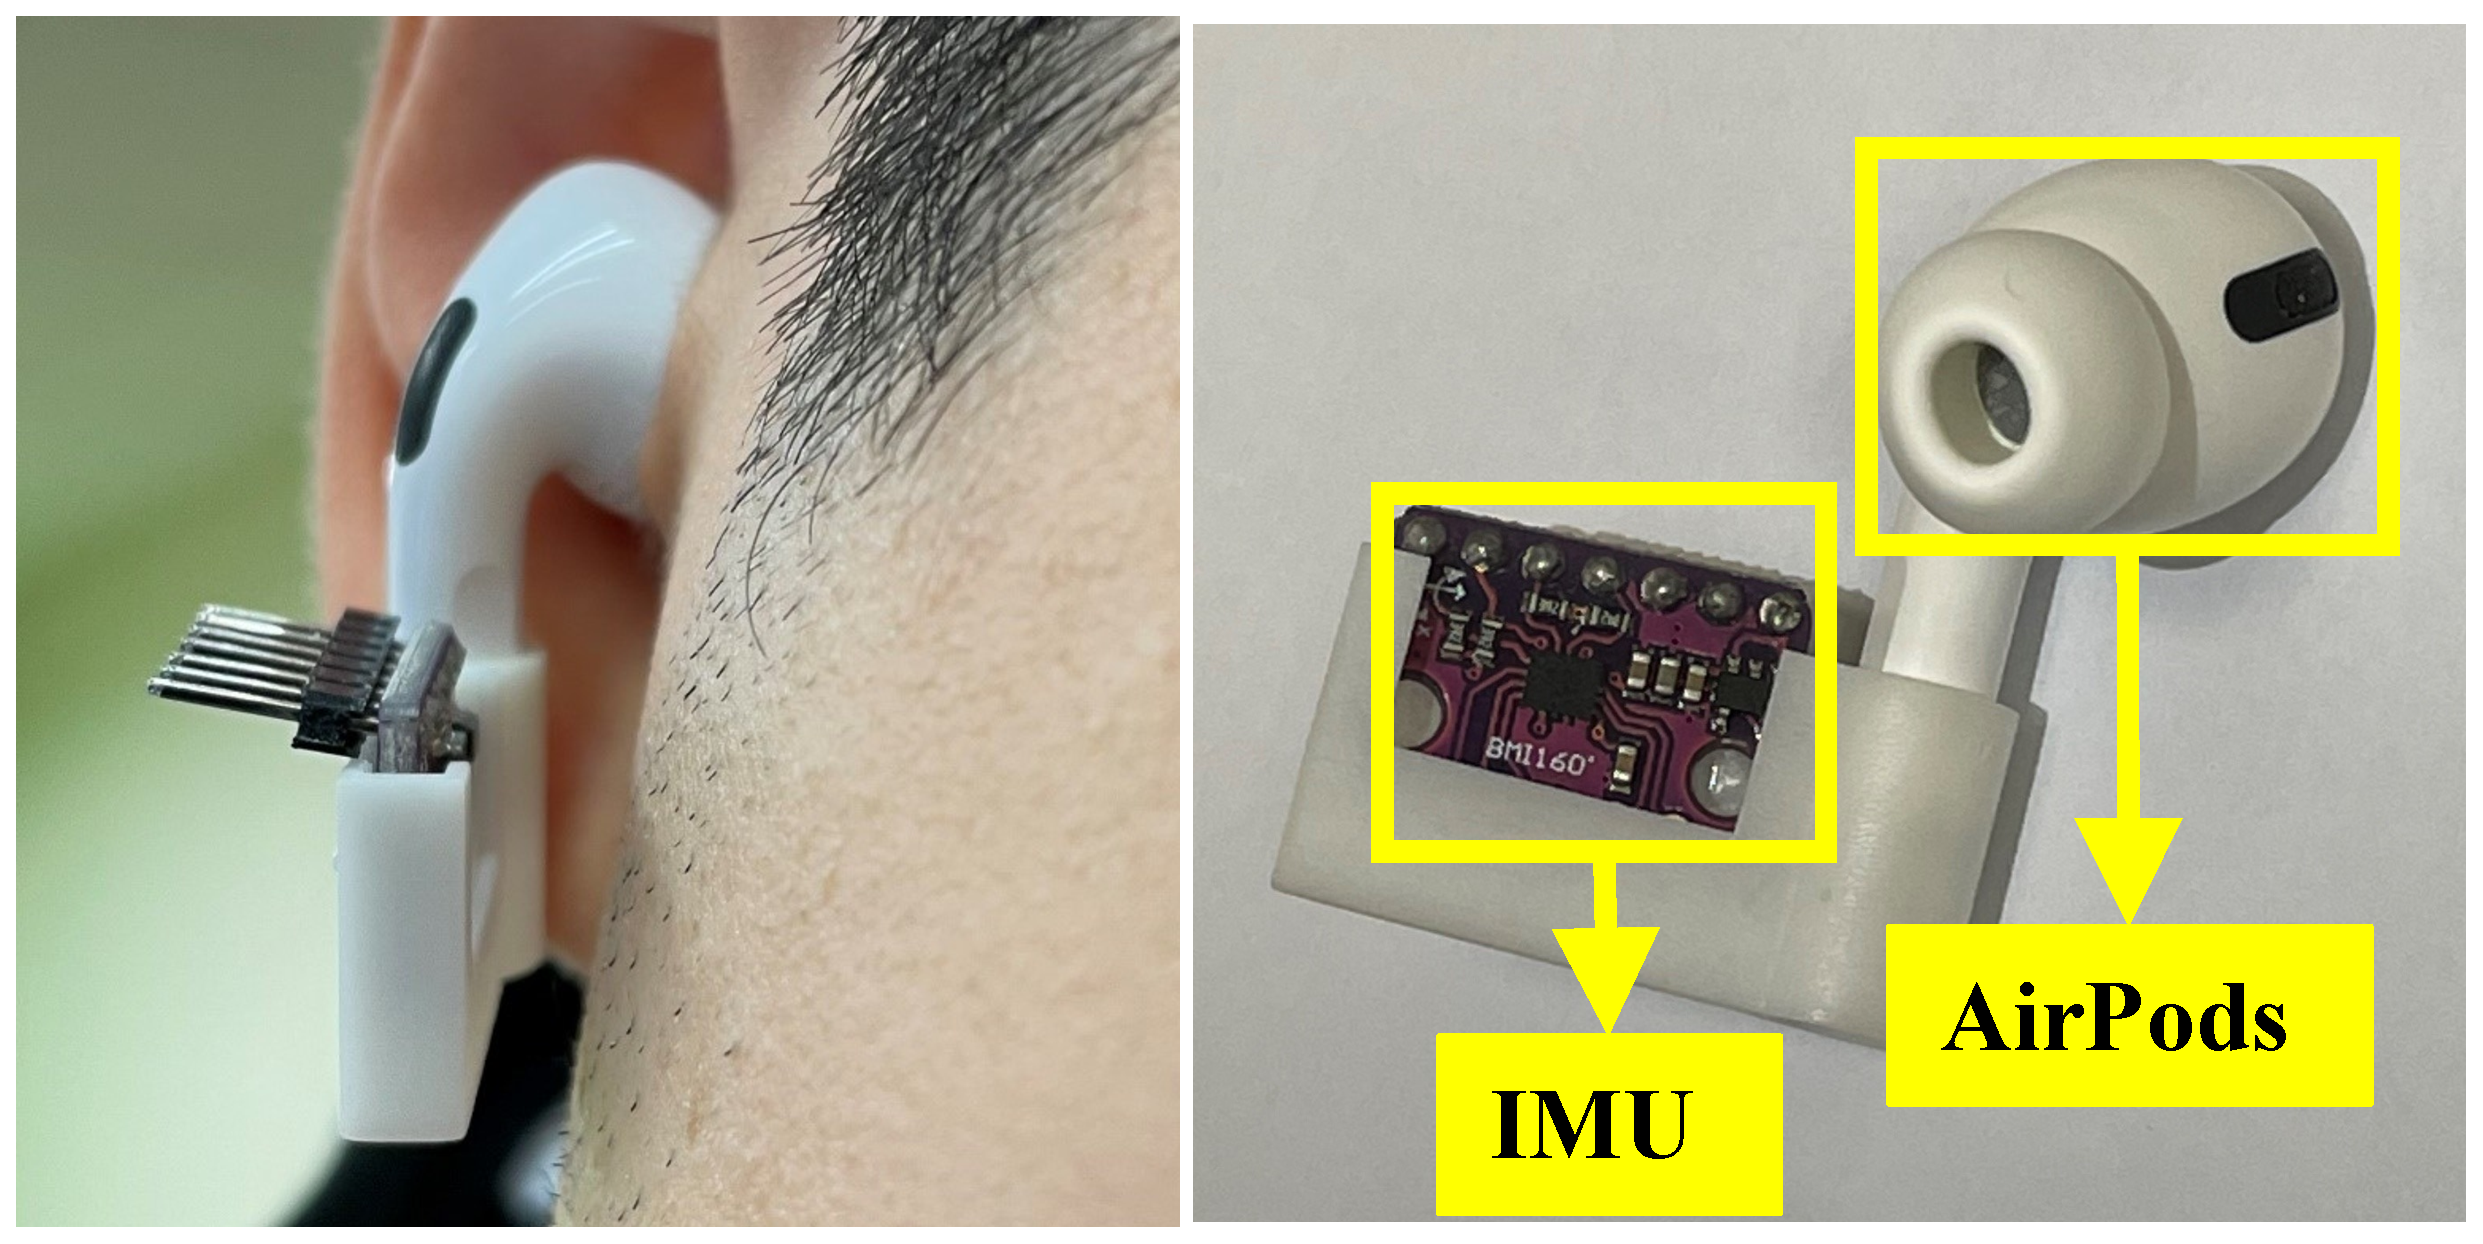
\includegraphics[width=\textwidth]{chapters/vibvoice/figure/earsense.eps}
    \caption{\emph{EarSense} with an Airpods Pro.}
    \label{fig:vibvoice_earsense-head}
  \end{subfigure}
  \begin{subfigure}{0.35\columnwidth}
    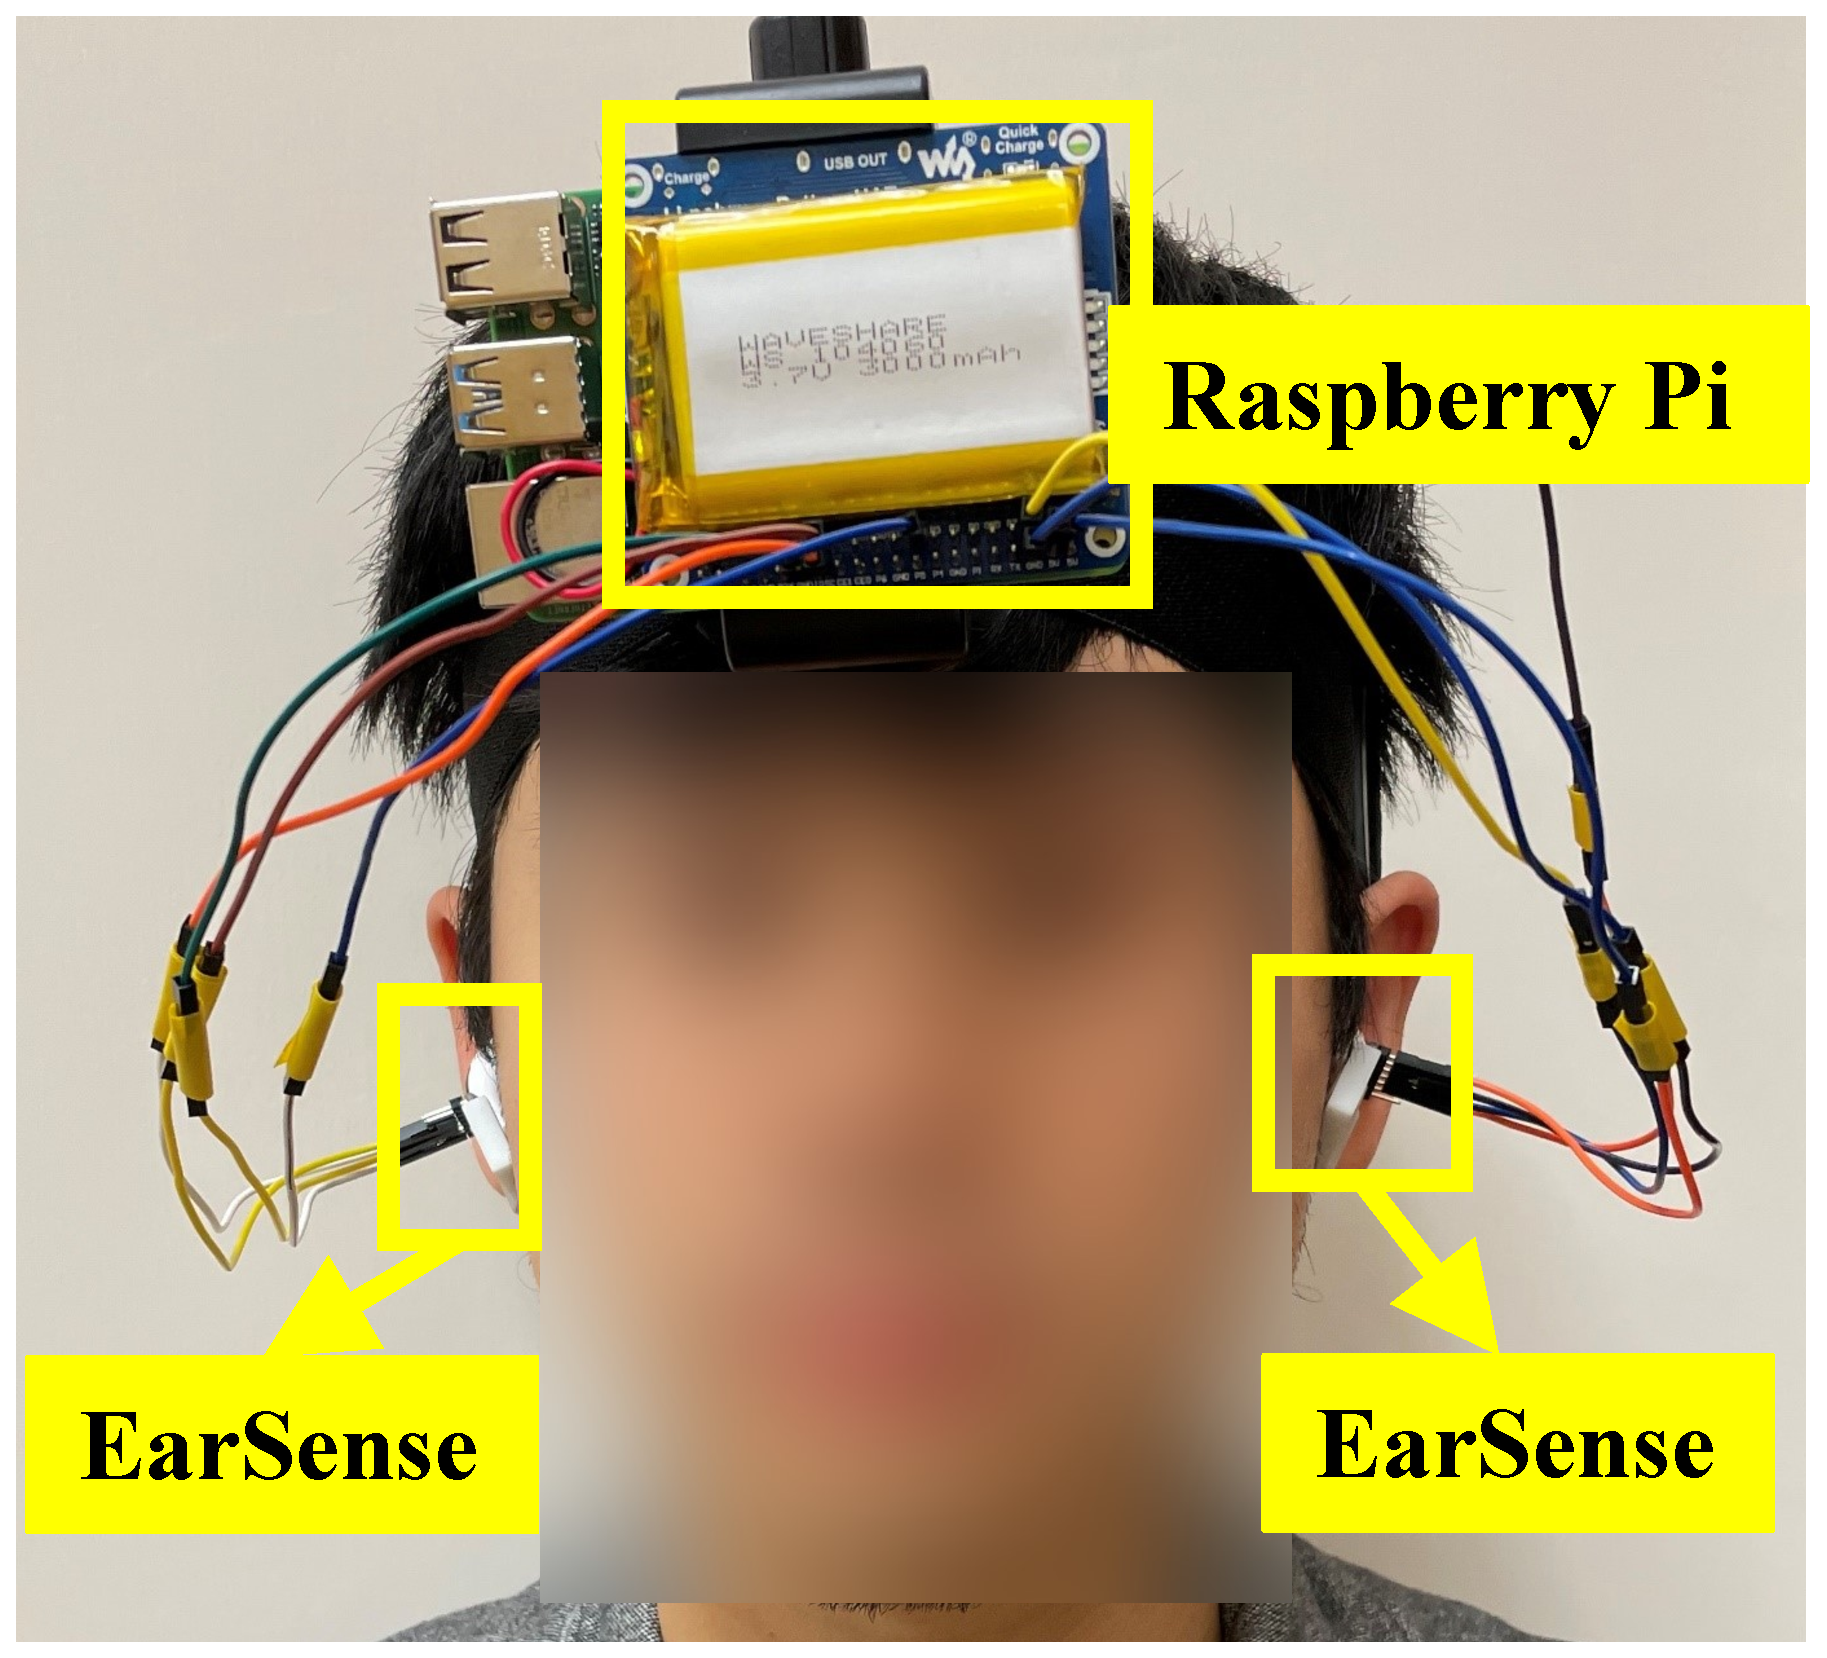
\includegraphics[width=\textwidth]{chapters/vibvoice/figure/people.eps}
    \caption{Test Setup.}
    \label{fig:vibvoice_earsense-people}
  \end{subfigure}
  \caption{\emph{EarSense} is an open-sourced data collector attachable to commercial HMWs for vibration sensing.}
  \label{fig:vibvoice_earsense}
\end{figure}

Fig. \ref{fig:vibvoice_earsense} shows the prototype of \textit{EarSense} \citep{dataset}, a new open-sourced sensing platform that houses an IMU sensor (Bosch BMI-160 \citep{Inertial63:online}) in a 3D-printed enclosure. EarSense has a flexible design that makes it attachable to commercial HMW devices (e.g., AirPods Pro). EarSense captures the same vibrations as the tested HMW and has no direct contact with the user's head (Fig. \ref{fig:vibvoice_earsense-head}).
We connect two EarSenses to a Raspberry Pi (RPi) with a battery for data collection.
Fig. \ref{fig:vibvoice_earsense-people} shows a volunteer wearing the device on the head to avoid excessive vibrations caused by the connecting wires.
A Python script on the RPi controls the EarSense(s) through the I2C protocol and stores the data for offline processing.
We use only the three-axis accelerometer provided by the IMU chip because the gyroscope and magnetometer are less related to the vibration.
The default sampling rates of the microphone and the accelerometer are $16\,\text{kHz}$ and $1.6\,\text{kHz}$, respectively. Since commercial earphones like AirPods Pro do not support two-channel audio recording, EarSense records audio in a mono channel.
We apply the L2 norm to the spectrograms of three-axis acceleration to extract vibration intensity and avoid the impact of wearing position and user motion.

\subsubsection{Measurements of Bone-Conducted Vibrations}
\label{sec:vibvoice_measurement}
We measure the differences between audio and bone-conducted vibrations with EarSense under various settings—specifically, competing speakers and user motion. In each experiment, we ask a volunteer to wear Apple AirPods Pro with EarSense attached (Fig. \ref{fig:vibvoice_earsense-people}) in a meeting room of size $10~\text{m}^2$. 
\begin{figure}
    \begin{subfigure}{0.46\columnwidth}
        \centering
        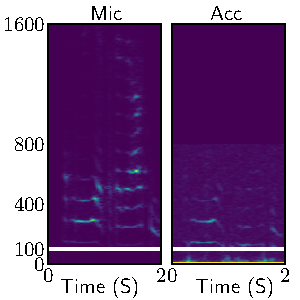
\includegraphics[width=1\textwidth]{chapters/vibvoice/figure/clean.pdf}
        \caption{The user is talking with no noise.}
        \label{fig:vibvoice_nospeaker}
        \end{subfigure}
        \hspace{.5em}
    \begin{subfigure}{0.46\columnwidth}
        \centering
        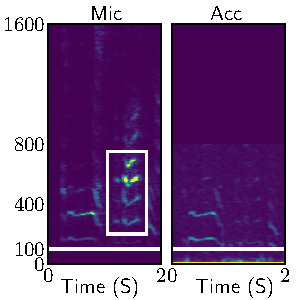
\includegraphics[width=1\textwidth]{chapters/vibvoice/figure/noise.pdf}
        \caption{The user is talking with a competing speaker.}
        \label{fig:vibvoice_speaker}
         \end{subfigure}
    \caption{Impact of the competing speaker.}
    \label{fig:vibvoice_competing-speaker}
\end{figure}

\noindent\textbf{Competing speaker.}
First, we ask the user to sit in the meeting room and speak while a loudspeaker plays pre-recorded speech one meter from the user as the competing speaker. Competing speakers are among the most challenging environmental noises for HMWs because their spectra resemble speech, making them difficult for noise suppression algorithms.
We set the competing speaker's volume similar to the user's, yielding an SNR of 3 dB. Volume alone cannot separate the sources since the two speeches are mixed.
Fig. \ref{fig:vibvoice_nospeaker} and Fig. \ref{fig:vibvoice_speaker} show the spectrograms of microphone audio and acceleration when the environment is quiet or contains a competing speaker when the user is talking, respectively.
We show spectrograms up to $1.6\,\text{kHz}$ since the microphone has little energy above this band, and the accelerometer senses signals only up to $800\,\text{Hz}$.
The spectrograms show that acceleration has lower signal energy than microphone audio since acoustic vibration attenuates during bone conduction, especially for high-frequency vibrations. Compared with the silent environment, the audio spectrogram of microphone audio with a competing speaker shows strong distortions, as highlighted with the white box in Fig. \ref{fig:vibvoice_speaker}. However, the accelerometer spectrograms do not show this phenomenon because the competing speaker cannot produce bone-conducted vibrations.
In summary, the accelerometer captures the user's voice through bone conduction while excluding airborne environmental sounds, which is ideal for speech enhancement.

\noindent\textbf{User motion.}
We also measure noise caused by the user's motion by asking the volunteer to walk while talking. Fig. \ref{fig:vibvoice_walk} shows that walking induces low-frequency noise in acceleration. The green boxes show zoomed-in signals below $100\,\text{Hz}$. We observe clear periodic fluctuations at low frequency (i.e., $< 50\,\text{Hz}$), caused by steps.
In summary, user motion primarily affects acceleration at lower frequencies and does not affect our speech enhancement.
We also observe slight low-frequency fluctuation in acceleration in Fig. \ref{fig:vibvoice_competing-speaker}, although the volunteer is asked to stand still in this experiment. Since most human speech is above $85~\text{Hz}$ \citep{Voicefre75:online}, removing low-frequency audio (i.e., the white horizontal lines in Fig. \ref{fig:vibvoice_competing-speaker}) can effectively reduce motion interference.

\begin{figure}
\begin{minipage}[t]{0.46\columnwidth}
     \centering
        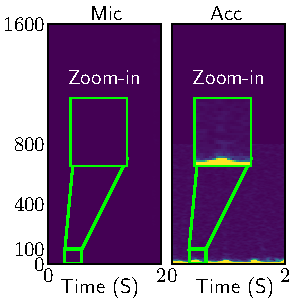
\includegraphics[width=1\textwidth]{chapters/vibvoice/figure/notalk.pdf}
        \caption{Spectrograms of microphone and acceleration when the user is walking.}
        \label{fig:vibvoice_walk}
\end{minipage}
\hfill
   \begin{minipage}[t]{0.48\columnwidth}
     \centering
       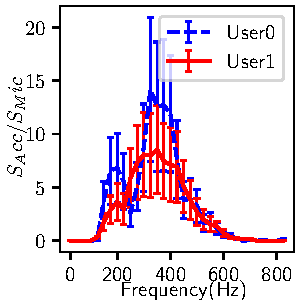
\includegraphics[width=1\textwidth]{chapters/vibvoice/figure/transfer_variance.pdf}
    \caption{Frequency responses of two users' bone-conducted vibrations.}
    %\vspace{-2em}
    \label{fig:vibvoice_bcf}
\end{minipage}
\end{figure}

\noindent\textbf{Frequency Response.}
We further explore the frequency response of bone-conducted vibrations among users. 
Specifically, we measure the frequency response as follows: first, we compute the spectra of audio and vibration data, denoted by $S_{\mathrm{Mic}}$ and $S_{\mathrm{Acc}}$, respectively. Then, we compute the Bone Conduction Function (BCF) as $S_{\mathrm{Acc}}/S_{\mathrm{Mic}}$ at every frequency band. Fig. \ref{fig:vibvoice_bcf} shows two volunteers' frequency responses, with error bars representing averages and variances.
Acceleration shows higher sensitivity than the microphone within $200$–$500\,\text{Hz}$, and lower sensitivity above $500\,\text{Hz}$ due to absorption by the skull. 
Additionally, the frequency response shows significant similarity among users, indicating generalization.
Hence, the BCF should consider inter-person diversity as well as inter-person similarity.

\begin{figure}
\begin{minipage}[t]{0.48\columnwidth}
     \centering
    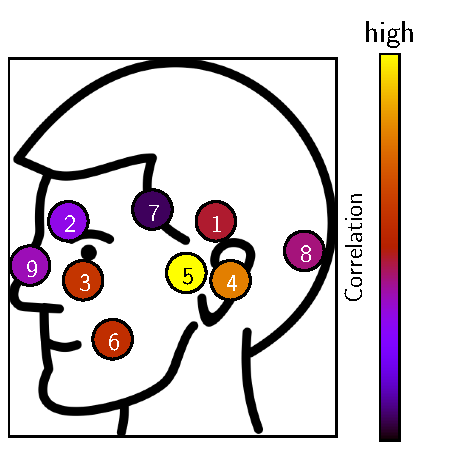
\includegraphics[width=\textwidth]{chapters/vibvoice/figure/correlation.pdf}
    \caption{Intensities of received bone-conducted vibrations on ten locations of the head.}
    \label{fig:vibvoice_head_positison}
\end{minipage}
\hfill
   \begin{minipage}[t]{0.48\columnwidth}
     \centering
    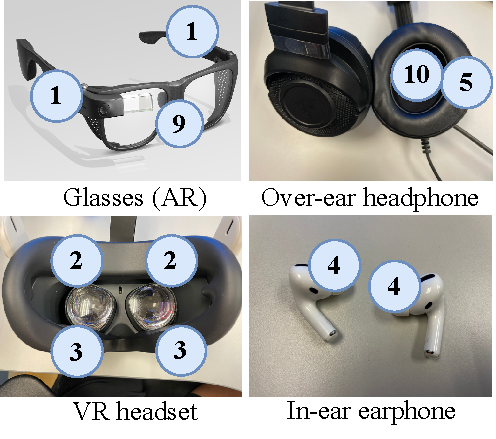
\includegraphics[width=\textwidth]{chapters/vibvoice/figure/devices.pdf}
    \caption{Potential placements on devices.}
    \label{fig:vibvoice_devices}
\end{minipage}
\end{figure}
\noindent\textbf{Locations on the head.}
Bone-conducted vibration exists at various locations on the head. 
As shown in Fig. \ref{fig:vibvoice_head_positison}, we select ten unique locations of interest on the head and measure the intensities of received bone-conducted vibrations. The nine facial/head locations are \#1 \emph{upper ear}, \#2 \emph{eyebrow}, \#3 \emph{cheekbones}, \#4 \emph{ear}, \#5 \emph{temporomandibular joint}, \#6 \emph{cheek}, \#7 \emph{temple}, \#8 \emph{back of the head}, and \#9 \emph{nose}. In addition, we tape EarSense on the interior of the pad of an over-ear headphone, denoted as \#10.
Among those positions, some are compatible with commercial HMWs like glasses, headphones, and VR headsets. Fig. \ref{fig:vibvoice_devices} illustrates the corresponding positions on HMWs. The numbers on the HMWs correspond to the locations in Fig. \ref{fig:vibvoice_head_positison}. 
We attach EarSense to the HMWs (when applicable) or on the face for all the following tests. 
We compute Pearson correlation coefficients between the audio and the acceleration on each location and mark the values using a color map in Fig. \ref{fig:vibvoice_head_positison}.
We observe that bone-conducted vibrations exist at most locations of the head. In particular, locations closer to the mouth show higher correlations, indicating a larger possibility of extracting clean speech. 

In summary, our measurements show that bone-conducted vibration has the following characteristics: a) it is robust to environmental voices and primarily captures the user's speech; b) user motion mainly generates vibrations lower than $85\,\text{Hz}$; c) it suppresses low- and high-frequency audio, with variations across and within users; and d) usable signals can be received from multiple locations on the head.

\subsection{Human Activity Recognition}
\label{sec:egolog_measurement}
As discussed in Sec. \ref{sec:egolog_intro}, multimodal HAR on mobile devices faces three main challenges: 1) lack of scenario awareness, 2) sensitivity to ambient noise, and 3) fusion collapse. To explore these challenges and assess potential solutions, we conduct a series of experiments.

\begin{figure}
    \centering
    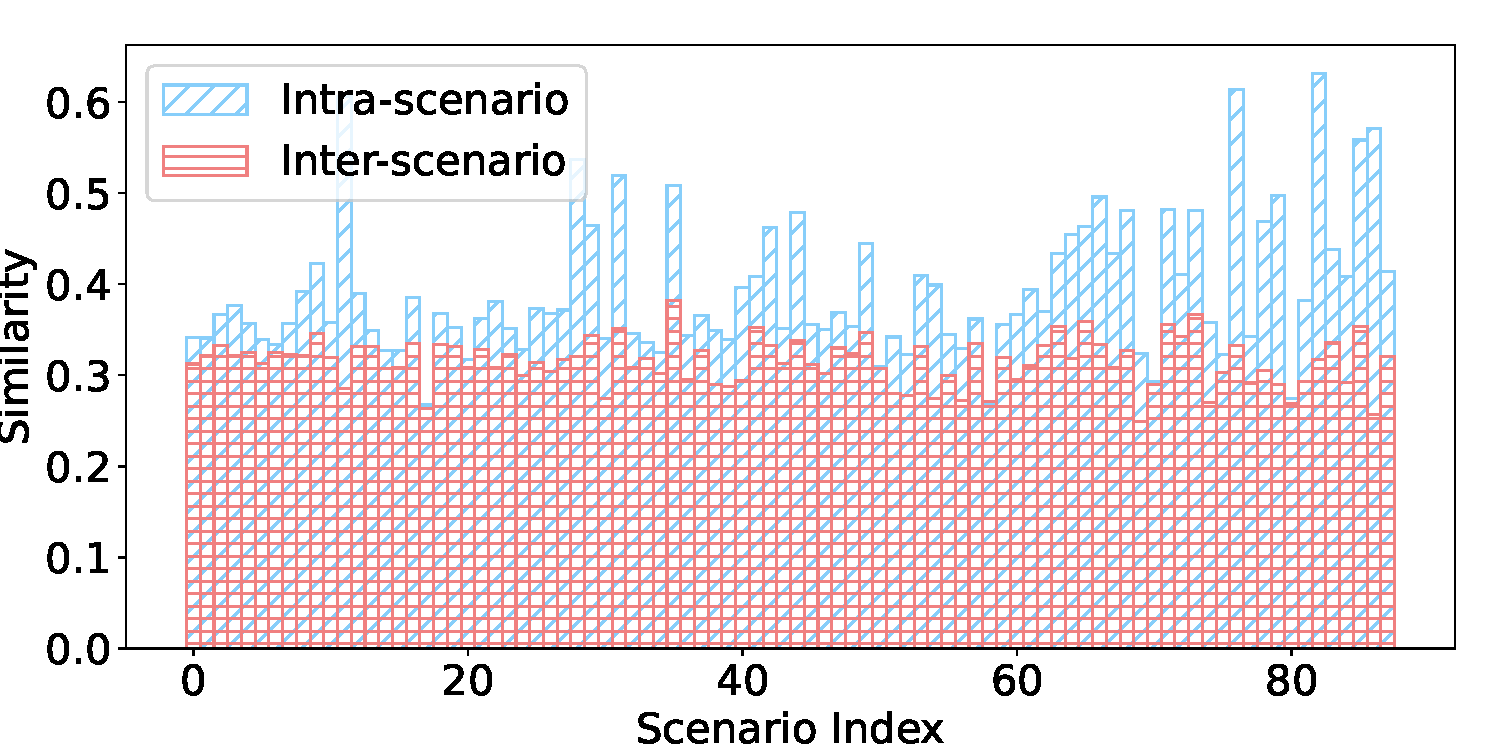
\includegraphics[width=0.8\linewidth]{chapters/egolog/figs/scenario_similarity.pdf}
    \vspace{-1em}
    \caption{Motivation for scenario understanding: 
    The similarity of embeddings for intra- and inter-scenario activities.}
    \label{fig:egolog_scenario_similarity}
    \vspace{-1em}
\end{figure}

\subsubsection{Scenario}
\label{subsec:scenario}
Scenario information refers to long-time activities (e.g., playing with a pet or working at home) that reflect the user's real-world behavior. Capturing such scenarios in datasets is challenging, as it requires volunteers to perform activities naturally, mimicking real-life conditions. Generally, scenario is the ensemble of multiple related and continuous activities with a realistic distribution, reflecting meaningful interactions with the environment.

To investigate the impact of scenario information on HAR, we utilize the Ego4D dataset \citep{grauman2022ego4d}, which captures real-world activities through smart glasses equipped with IMU and audio sensors. The dataset provides annotations at both the window level (every 10 seconds) and the video level, represented as plain text. We treat window-level annotations as activity labels and video-level annotations as scenario labels, reflecting prolonged activities. To examine scenario properties, we employ Sentence-BERT \citep{reimers2019sentence} to generate text embeddings for activities across 91 scenarios. We then compute activity similarity both within scenarios (intra-scenario) and between scenarios (inter-scenario). Intra-scenario similarity measures the similarity of activities within the same scenario, while inter-scenario similarity compares an activity from one scenario to a randomly selected activity from a different scenario.

The results in Fig.~\ref{fig:egolog_scenario_similarity} reveal that intra-scenario similarity is over 20\% higher than inter-scenario similarity. This suggests that each scenario has a distinct distribution of activities and effectively represents the user's daily log over a longer time frame.
Additionally, inter-scenario similarity is generally above 0.3, indicating that many basic activities (such as sitting and walking) are common across scenarios. Therefore, it is crucial to reduce the influence of these basic activities in scenario recognition.


In summary, the study on the in-the-wild dataset indicates unique activity distributions per scenario, which can be leveraged to recognize scenarios by identifying scenario-specific activities.

\subsubsection{Sound Location }
\label{subsec:embodied}
\begin{figure}
    \centering
    \begin{minipage}{0.48\linewidth}
        \centering
       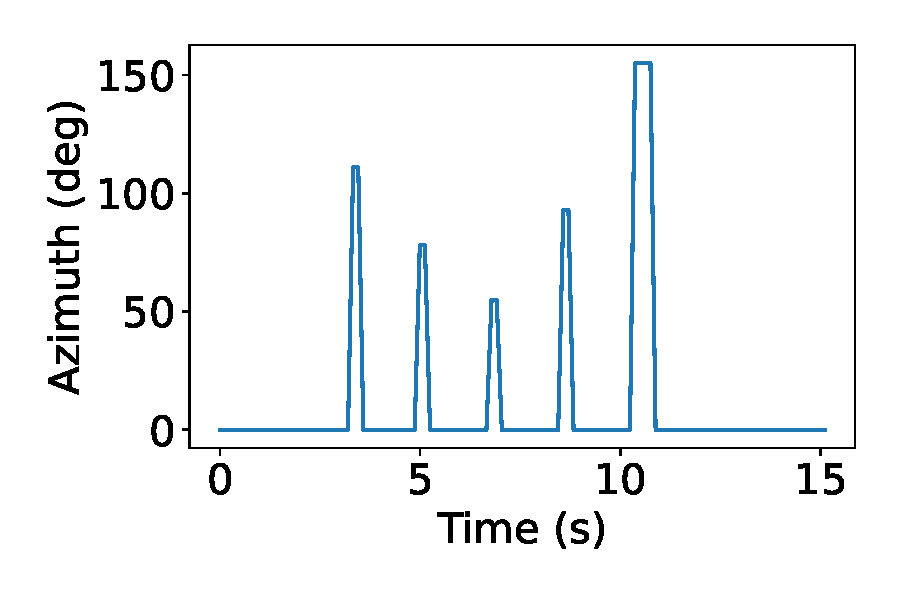
\includegraphics[width=\linewidth]{chapters/egolog/figs/baseline_result.pdf}
        \caption{Sound localization under motion \citep{schmidt1986multiple}}
        \label{fig:egolog_loc_move}
    \end{minipage}
    \hfill
    \begin{minipage}{0.48\linewidth}
        \centering
        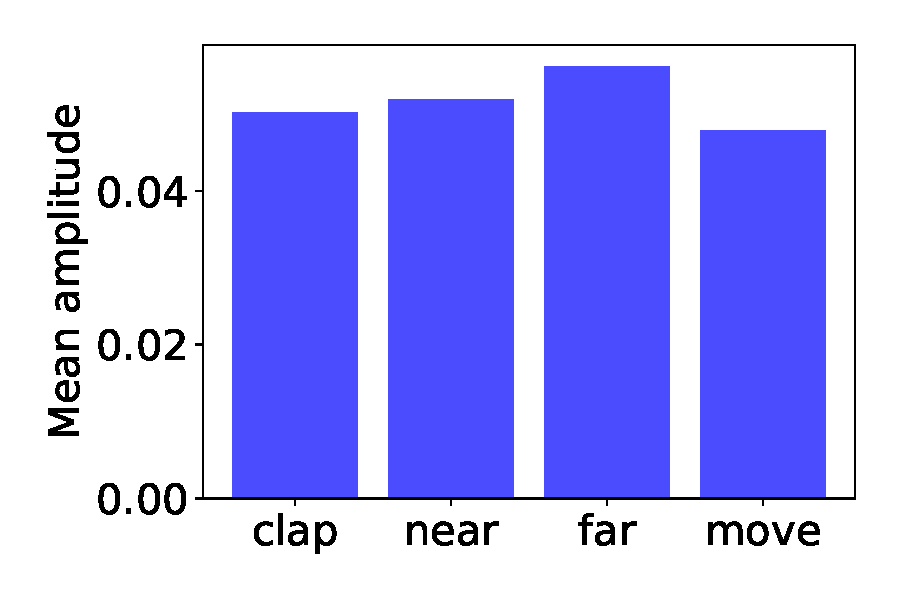
\includegraphics[width=\linewidth]{chapters/egolog/figs/amplitude.pdf}
        \caption{Sound volume may not relate to distance.}
        \label{fig:egolog_amplitude}
    \end{minipage}    
    \vspace{-1em}
\end{figure}

\begin{figure}
    \centering
    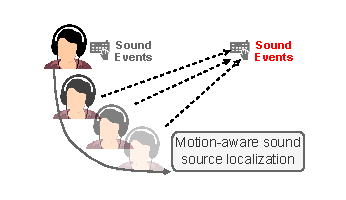
\includegraphics[width=0.75\linewidth]{chapters/egolog/figs/spatial_motivation.pdf}
    \vspace{-1em}
    \caption{Motivation for spatial understanding: estimate the distance of a sound event via motion.}
    \vspace{-1em}
    \label{fig:egolog_motivation_localization}
\end{figure}

In practice, recorded audio often includes far-field sound sources that are unrelated to the user’s activities, underscoring the importance of sound localization for effective HAR. Wearables that are consistently worn on the user’s head provide a stable and reliable position for capturing detailed ambient sound information. Additionally, modern wearables feature multi-channel recording capabilities, enhancing their spatial sensing potential.
In the following, we divide sound localization into direction and distance estimation, which we discuss as follows.

Estimating sound direction is mature but remains challenging. Accuracy depends heavily on the number of microphones, which is limited in most commercial devices. In common stereo settings, two main problems arise: directional deviation (especially front–back confusion) and estimating sound distance, as illustrated in Fig. \ref{fig:egolog_motivation_localization}.
We envision addressing these challenges via motion compensation. Specifically, we can aggregate consecutive localization results along with user (microphone) movement to refine direction estimates and infer distance.

To illustrate, we positioned a sound source in front of the user and utilized a binaural microphone along with the algorithm from \citep{schmidt1986multiple} to estimate direction of arrival, as shown in Fig. \ref{fig:egolog_loc_move}. The user was instructed to move slightly and naturally. Estimates were not satisfactory, fluctuating around the true value of 90 degrees. To validate whether sound volume differentiates near vs. far, we conducted an experiment with varying source distances. As shown in Fig. \ref{fig:egolog_amplitude}, there was no notable volume difference between cases, indicating that volume alone is an unreliable indicator of distance. The final bar in Fig. \ref{fig:egolog_amplitude} reveals that user movement slightly affects amplitude. Multiple sound sources can further complicate volume patterns.

\subsubsection{Multi-modal Fusion }
\label{subsec:measure-fuse}

\begin{figure}
    \centering
     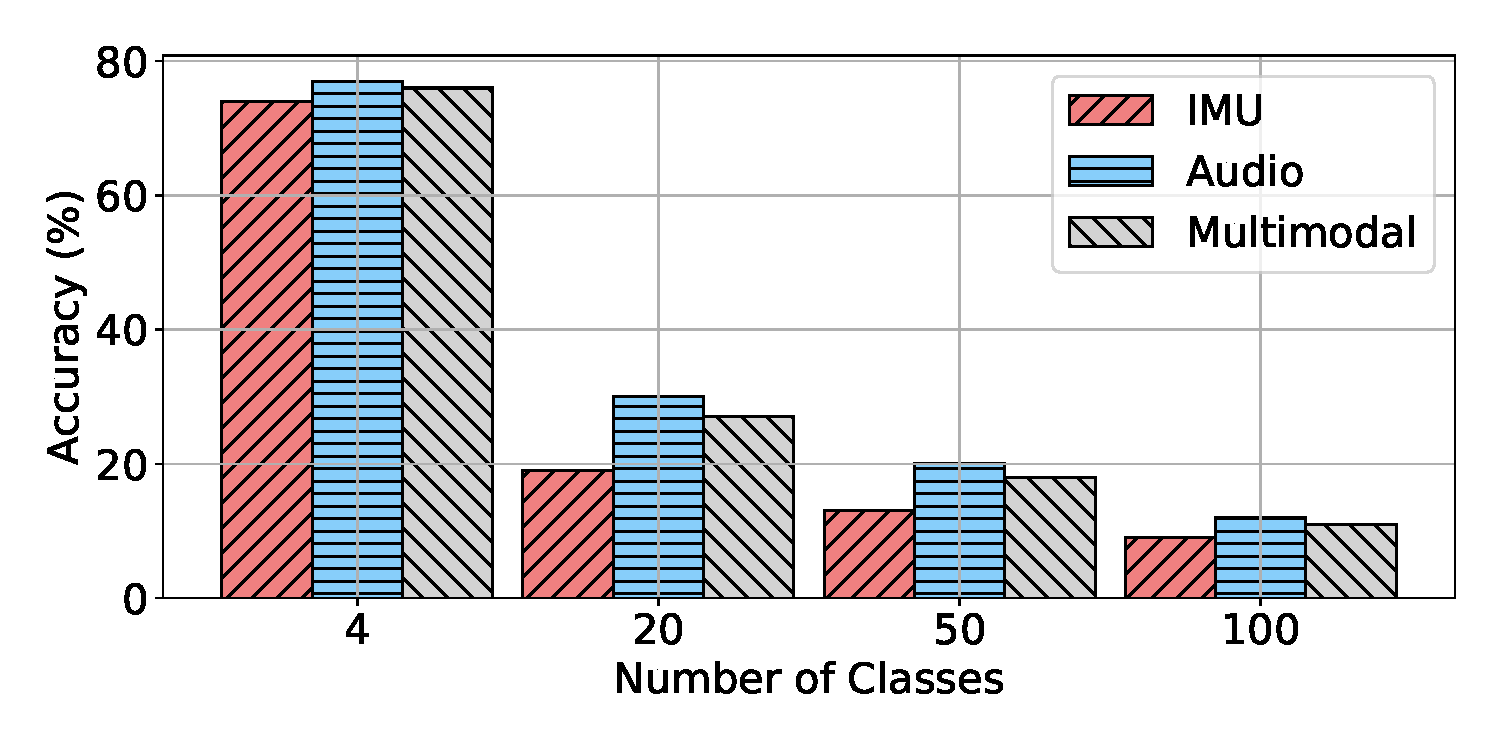
\includegraphics[width=.75\linewidth]{chapters/egolog/figs/num_class.pdf}
     \vspace{-1em}
      \caption{The performance of an existing activity recognition with different class numbers and modalities.}
    \label{fig:egolog_num_class}
    \vspace{-1em}
\end{figure}

To investigate scalability bottlenecks in activity recognition using wearables, we trained unimodal supervised models with audio and IMU data on the Ego4D episodic memory subset (200 activity classes). We used EfficientAT~\citep{schmid2023efficient} for audio and LIMU-BERT~\citep{xu2021limu} for IMU as feature extraction backbones, comparing them to a multi-modal model via late fusion. Activities were clustered into varying class numbers using Sentence-BERT~\citep{reimers2019sentence} embeddings and K-Means~\citep{macqueen1967some}, following MMG-Ego4D~\citep{gong2023mmg}. Results (Fig.~\ref{fig:egolog_num_class}) show a significant performance drop as class numbers increase, indicating challenges in recognizing diverse activities with audio or IMU alone. Multimodal fusion often underperforms unimodal models, suggesting ineffective extraction of complementary features at larger scales.

\begin{figure}
    \centering
    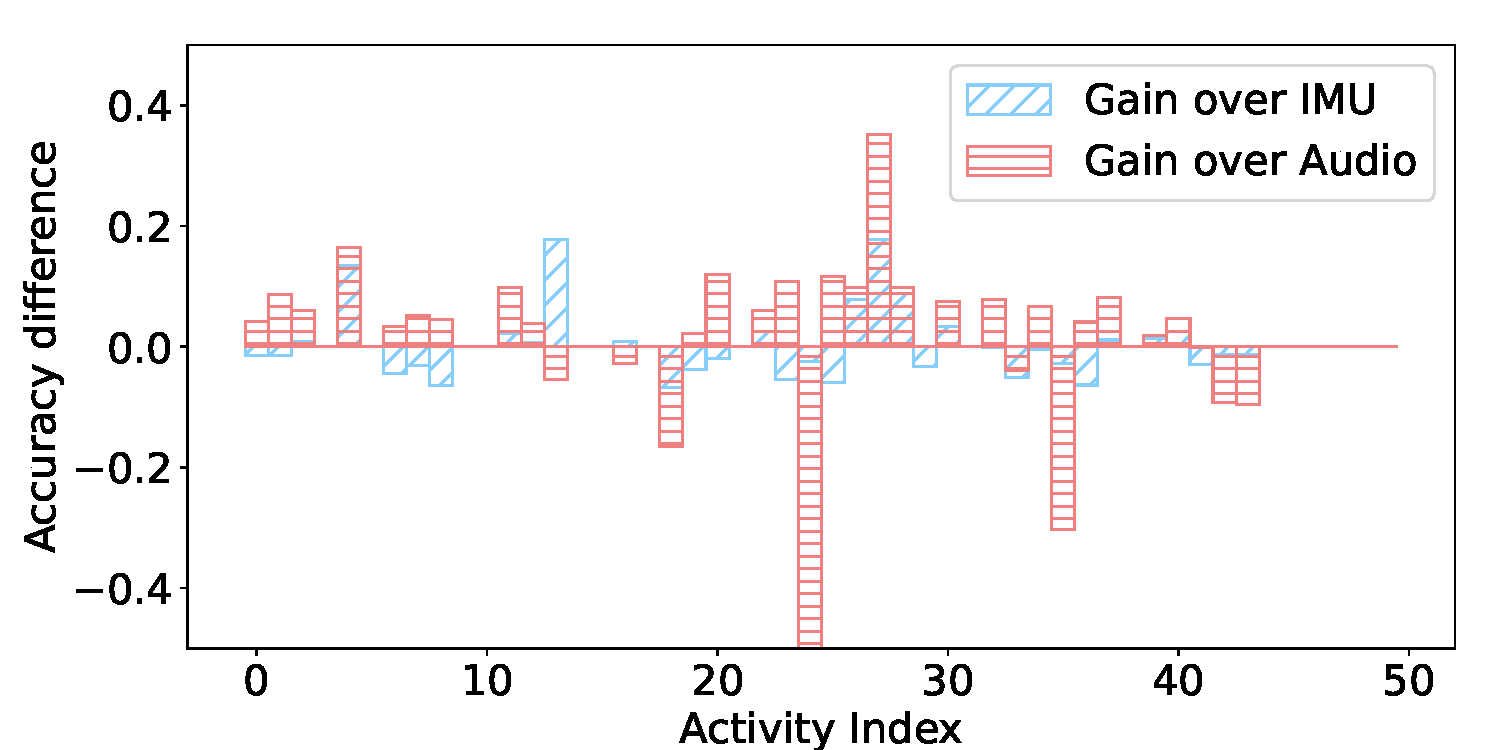
\includegraphics[width=.75\linewidth]{chapters/egolog/figs/activity_diff.pdf}
    \vspace{-1em}
    \caption{Performance gain from multi-modal fusion.}
    \label{fig:egolog_acc_gap}
    \vspace{-1em}
\end{figure}

Previous work~\citep{mollyn2022samosa} demonstrates that multimodal learning can outperform unimodal models due to complementary information.
However, this does not always apply: another study~\citep{gong2023mmg} finds multimodal audio+IMU learning on Ego4D can perform worse than single-modality solutions. To investigate, we compare the accuracy of multimodal and unimodal models for each class (Fig. \ref{fig:egolog_acc_gap}). We observe that the advantages of multimodal fusion fluctuate across classes and modalities, indicating that supervised multimodal learning does not automatically select the right modality and may fail to benefit from fusion.


To investigate the effectiveness of LLMs in alleviating the problem, we employ ImageBind-LLM \citep{han2023imagebind}, which converts both modalities into features and conditions them with text embeddings. We instruct the model with: "<sensor> According to the audio and IMU reading on the user's earphone, what is the user's activity?", where <sensor> refers to the placement of sensor features. Because LLM outputs can be random, we also add a prompt to force it to output one of the potential activities. To reduce complexity, we select the top 30 activities in the Ego4D episodic memory subset. The BERT scores of ImageBind-LLM are 0.04 (precision), 0.07 (recall), and 0.05 (F1), which are too low for practical use. Inspecting outputs suggests the LLM may not fully understand the fusion task.
Furthermore, we investigate whether fine-tuning can resolve the problem by training an adapter~\citep{zhang2023llamaadapter} for ImageBind-LLM. The adapted LLM achieves BERT scores of 0.47 (precision), 0.46 (recall), and 0.47 (F1). Although much improved, performance remains below usability and is far from practical.


\chapter{VibVoice: Towards bone-conducted vibration speech enhancement on head-mounted wearables}\label{ch:vibvoice}
This chapter presents VibVoice, an end-to-end multimodal speech enhancement system for earphone-class head-mounted wearables. VibVoice fuses bone-conducted vibration sensed by an on-device IMU with microphone audio to isolate the wearer's voice. The chapter describes the motivation, system design, and evaluation of VibVoice.


\section{Introduction}
\label{sec:intro}
% Backgound
\begin{figure}
    \centering
    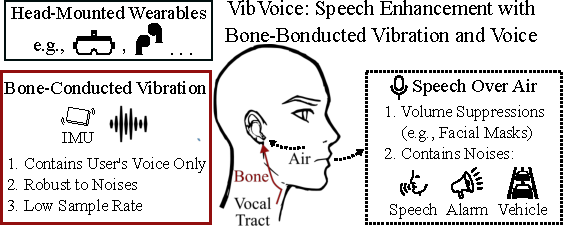
\includegraphics[width=\columnwidth]{chapters/vibvoice/figure/intro.pdf}
        %\vspace{-1em}
    \caption{VibVoice enhances speech quality of head-mounted wearables by extracting the user's clear voice from the bone-conducted vibrations.}
    \label{fig:intro}
\end{figure}
Head-mounted wearables, or HMWs, are smart devices that can be put on users' heads or ears, which include True Wireless Stereo (TWS) earphones, VR/AR headsets, and smart glasses. HMWs are equipped with several sensors and run various applications like VR/AR, motion recognition, and voice assistants. Represented by TWS earphones like the Apple Airpods series, the shipment of HMWs has grown as the largest category among all wearable devices, estimated to be more than $273$ million units worldwide in 2023 \citep{wearable-stat}. 
Manufacturers are adding various functions to HMWs. For example, some HMWs (especially earphones and headphones) support active noise cancellation (ANC) to improve the listening experience. On the speech side, voice-related applications using HMW s microphones are among the most frequently used. 

For example, an increasing number of people make phone calls with TWS earphones.
Through voice commands, users can also interact with voice assistants (e.g., Siri and Alexa). 
However, the speech quality on HMWs is unsatisfactory due to the following challenges:
First, most HMWs adopt omnidirectional microphones that can receive audio from any angle, leading to extra environmental noises.
Second, although most HMWs are equipped with multiple microphones to form an array and remove noises based on beamforming, the microphones on HMWs are too close to achieving a satisfying performance. 
Third, the speech audio is significantly suppressed when it reaches the HMWs as the HMWs are usually far away from the user's mouth.
Lastly, the worldwide pandemic forces people to wear masks, which can further reduce the audio intensity.

% Existing approach
Various approaches have been developed for speech enhancement. Signal processing-based methods \citep{ephraim1995signal} remove noises based on their statistical models. However, these approaches cannot handle complex environments. Microphone beamforming \citep{yousefian2014hybrid,ji2017coherence} removes noises based on their directions. But they fail to distinguish the speaker's voice and noise when the microphones are placed too close. Several research \citep{subakan2021attention, zhang2021microphone, chatterjee2022clearbuds} adopt deep neural networks (DNNs) to improve speech quality. However, their performance varies when the domain changes.  
Except for the audio-only solution, several works leverage other modalities like contact sensors \citep{gupta2018precision}, vibration sensor \citep{maruri2018v}, camera \citep{ gao2021visualvoice}, mm-Wave Radar \citep{ozturk2021radiomic, li2020vocalprint, liu2021wavoice}, ultrasonic sensing \citep{sun2021ultrase, zhang2021sensing}, and Lidar \citep{sami2020spying}, which introduce additional hardware requirements or user overhead to existing HMWs.

% Technical Challenges
Inertial Measurement Unit (IMU) is a common sensor on most HMWs and can capture audio with a direct connection with the speaker \citep{ba2020learning, wang2021audio}. Since HMWs are well connected to the user's head, the IMU accelerometer can sense the vibrations caused by the speaker's voice through the skull's bone conduction. The bone-conducted vibration contains speech from the user only without environmental noises or voices. However, the accelerometer on HMWs has a low sample rate (e.g., $1.6~\text{kHz}$) due to the limited size and energy consumption, which is not enough to recover the human's voice (e.g., up to $3.4~\text{kHz}$ \citep{Voicefre75:online}). 

We propose \textit{VibVoice}, the first end-to-end multi-modal speech enhancement system for HMWs using the bone conduction from the vibration to the audio. The design of VibVoice fits mobile devices, considering the on-device sensor, execution latency, and communication overhead.
VibVoice exploits the complementary characteristics of the two modalities: the acceleration has a low sample rate covering a partial audible spectrum but with no environmental noises. The microphone has a high sample rate covering the whole audible spectrum but is mixed with ambient voice and noises. Such a combination of modalities provides a stable reference for extracting the target speech.
VibVoice uses a DNN to reconstruct clean speech with two encoders and decoders for processing the data from two modalities, respectively. VibVoice faces three major technical challenges as follows:

\noindent\textbf{Lack of paired labeled acceleration and audio.}
Collecting a paired multi-modal dataset is labor-intensive. Although there are public datasets of either acceleration or audio, none has the paired data on head-mounted wearables. 
Collecting such a paired dataset on a large scale can introduce excessive overheads, such as recruiting diverse volunteers and recording hundreds of hours of audio with annotations. 

\noindent\textbf{Fusion of data with different modalities and sample rates.}
Microphone audio has much richer information than acceleration data due to the higher sample rate. As a result, the DNN is prone to overfitting and may ignore the data input of acceleration. 
Therefore, during the training of DNN, we require a special training strategy to avoid overfitting and two dedicated losses to balance the weights of the two modalities.

\noindent\textbf{Practical concern for deployment.} 
Deploying deep learning speech enhancement in the real world is non-trivial due to the variance among people's voice and bone conduction channels.    
Even though some users may tolerate a rapid data collection phase before use, the amount and quality of the collected data are not guaranteed for training a high-performance model.

To overcome the above challenges, we design VibVoice based on our extensive measurements of the bone-conduction effects on real-world data. We conclude our contributions as follows:
\begin{itemize}
    \item  We propose a novel estimation approach to model Bone Conduction Function with a limited dataset to augment paired acceleration and audio based on a large public audio dataset. The augmented paired dataset can be used for model training. 
    \item We design a two-branch DNN that a) recovers the speech-related information from the acceleration signal with a low sample rate, b) extracts the clean speech from contaminated audio with the help of the acceleration signal, and c) has a lightweight design and can be run on the mobile device with low latency.
    \item We collect a two-modal dataset and evaluate VibVoice on a self-designed platform, \emph{EarSense}, equipped with an accelerometer and a microphone to acquire paired acceleration and audio data simultaneously. The dataset and the design of data collector are open-sourced.
\end{itemize}

We evaluate VibVoice on a paired acceleration and microphone from 15 volunteers. We test VibVoice's performance on the offline synthetic noise dataset and the concurrent noise dataset in various scenarios.
VibVoice achieves the best performance with 31 times less latency on mobile devices than the two strong baselines. In addition, data augmentation can reduce the requirement of paired data by more than 72 times.
We recruit 35 volunteers for a user study in which VibVoice is preferred by 87$\%$ users compared to the baseline.






% \section{Related work}\label{sec:relatedwork}

Speech enhancement is an essential function in voice communication that has received extensive attention. We categorize existing speech enhancement methods based on the input modalities, i.e., \textit{audio-only}, \textit{multi-modal}, as well as works sensing acoustic signals with other modalities.

\subsection{Audio-only Speech Enhancement}

\subsubsection{Model-driven}
Traditional speech enhancement either relies on assumptions of stationarity of signals, independence of speech, noise in the time-frequency domain \citep{ephraim1995signal}, or multiple omnidirectional microphones (e.g., a microphone array) to improve audio quality. The microphone array leverages the difference of arrival times (known as beamforming) toward each microphone to determine the direction of the speaker for speech enhancement \citep{yousefian2014hybrid,ji2017coherence}, and speech separation \citep{wood2017blind,kitamura2016determined}. However, those approaches cannot adapt to dealing with dynamic noises without prior knowledge.

\subsubsection{Machine Learning}
Recent studies adopt DNN \citep{subakan2021attention, zhang2021microphone, chatterjee2022clearbuds} for speech enhancement. The deep structure of neural networks can capture the inherited features of the target voice and potential noises based on a large training dataset.
DNN-based methods work on both single-channel audio \citep{subakan2021attention} and multi-channel audio with arbitrary microphones layouts \citep{zhang2021microphone}. ClearBuds \citep{chatterjee2022clearbuds} uses a DNN to process the stereo audio recorded by customized earbuds, which causes excessive communication overhead. ClearBuds filters noises based on the angles of sources, which does not work when a competing speaker stands at the same angle as the speaker.
Although audio-only deep learning speech enhancement achieves good performance, they rely on the training data domain and fail to enhance the speech quality with slim-volume audio.


\subsection{Multi-Modal Speech Enhancement}
Speech events involve the motions of several articulatory organs, such as the tongue, teeth, lips, jaw, and facial muscles, which can be leveraged for speech enhancement.

\subsubsection{Audio and Visual}
Researchers in \citep{michelsanti2021overview, gao2021visualvoice} leverage the video from a camera in the environment to correlate the audio and visual for speech enhancement and separation. 
These approaches leverage deep learning and cross-modal embeddings to extract the target speech from noises. However, a visual sensor like a camera is not always available in daily usage. 

\subsubsection{Audio and Wireless}
The authors in \citep{sun2021ultrase, zhang2021sensing} use the smartphone's speaker to transmit an inaudible acoustic signal (i.e., higher than $17\,\text{kHz}$) and simultaneously receive the echo reflected by moving lips, which can be used to enhance the noisy audio. 
\citep{liu2021wavoice, ozturk2021radiomic} use coupled mmWave and microphone recording for speech recognition rather than enhancing general speech contents. However, a mmWave radar is bulky and not common on HMWs, and the ultrasonic solution requires the user to fix the phone toward their mouth.

\subsubsection{Audio and IMU}
\label{subsubsec:related-audio-imu}
Some recent works have exploited the noiseless speech information from a bone conduction sensor or the accelerometer and the microphone recording for multi-modal speech enhancement. 

\citep{wang2022fusing} proposes a multi-modal DNN for speech enhancement trained by a self-collected dataset in Mandarin. However, the bandwidth of the vibration sensor is around 5~kHz, which is much higher than the one available on commercial devices \citep{Inertial63:online}.
SEANet \citep{tagliasacchi2020seanet} uses a DNN to augment acceleration from audio with the same transformation among all users. However, the diverse bone shapes can lead to different transformations and thus affect the generalizability. 
In addition, both works \citep{wang2022fusing, tagliasacchi2020seanet} focus on the design of deep learning models and fail to evaluate the systems with real-world noises and unseen users.

\subsection{Sensing Acoustic Signals}

IMU or piezoelectric sensor \citep{maruri2018v} can be installed on commercial devices to measure the contact sound, including unvoiced sound \citep{khanna2021jawsense}, breathing sounds \citep{gupta2018precision}, and eavesdropping smartphone/VR headset speaker \citep{ba2020learning, wang2021audio, su2021towards, shi2021face}. 
Although various contact sensing technologies are developed for acoustic sensing, they can classify keywords and events only rather than reconstructing the full-spectrum audio.
Previous works exploit remote acoustic sensing by correlating with several non-acoustic sensors (e.g., geophones, accelerometers, and gyroscopes) \citep{han2017pitchln}, using the LiDAR on a vacuum robot to predict acoustic signals from the vibrations on the surrounding surfaces \citep{sami2020spying}, or leveraging a mmWave Radar to achieve authentication \citep{li2020vocalprint}. 
However, they can only detect a given set of speech contents like digits and music. Measurements in \citep{anand2018speechless} show that smartphone's motion sensor can only capture air-conducted acoustic vibrations remotely in limited use cases.


\section{Background}\label{sec:background}
\subsection{Audio Recording on HMWs}
Although voice-related applications have been studied for decades, they usually exhibit unsatisfactory performance due to the following limitations. 
First, to save space and cost, most microphones installed on HMWs are omnidirectional instead of directional microphones due to their bulkiness and limitations in general use cases such as recording environmental sounds (e.g., Logitech 650e \citep{Logitech34:online}, around 100 USD). The omnidirectional microphones pick up audio from any angle, so they inevitably record the interference signals, especially the speech of a competing speaker close to the target user.
Second, although the latest HMWs usually equip multiple microphones for beamforming, the compact layout of the microphone array can impede the acoustic beamforming since the audio from different sources arrives at the microphones with only a minor time difference. Specifically, the microphone array's interval is much smaller than $\lambda_{min}/2$, while the $\lambda_{min}$ is the minimum wavelength of the interested frequency band.
Third, the microphones on HMWs are farther away from the user’s mouth than wired earphones or standalone microphones since they are usually inserted into the ears or mounted around the eyes. Therefore, the received intensity of the speech audio can be significantly suppressed due to the slim air transmission. 
Lastly, the worldwide pandemic forces people to wear facial masks, which can significantly reduce speech volume by up to 7dB \citep{porschmann2020impact}. 
Hence, seeking another available transmission channel for robust speech sensing is desirable.

\subsection{Bone-Conducted Vibrations}
Existing commercial headphones leverage bone conduction \citep{Bonecond79:online} for inner ear hearing assistance. In this paper, we focus on the transmission from the vocal cord to the head skull, which can be detected by the contact microphone \citep{Contactm68:online}. 
The noise-less feature of bone conduction sound has been discovered \citep{tagliasacchi2020seanet} with a bone conduction microphone. The professional bone-conducted microphone has also been applied in extremely harsh environments like battlefields or underwater applications \citep{EarBoneM7:online, BoneCond30:online}. However, there are still challenges to leveraging it for speech enhancement on HMWs. Firstly, as depicted in \citep{chang2016development, won2005estimating}, the propagation through the head is complicated, resulting in an unstable response even for the exact location. Secondly, although a professional bone-conducted microphone can capture a clear voice at a high sample rate, they are too expensive (e.g., 60 US dollars \citep{EarBoneM7:online, BoneCond30:online}) and not available on commercial HMWs.
The current commercial-level vibration sensor may not provide sufficient sample rate and precision, leading to frequency aliasing and a bad signal-noise ratio.
Some approaches tackle the problems by duplicating the signals of low-frequencies to high-frequency domain \citep{dietz2002spectral}, utilizing the time stretching to generate high-frequency harmony \citep{nagel2009harmonic}, or also trying to unfold the acceleration signals from low sample rate using deep learning \citep{wang2021audio}. However, these approaches are far from achieving satisfying performance because the speech in high frequency contains extra information than that in low frequency.
As a result, a simple recovery on the high-frequency part can amplify the noise of acceleration and degrade the quality of the generated audio.
\section{Background}
\label{sec:vibvoice_background}
This section introduces EarSense, an open-source wearable platform with a sensing setup similar to current commercial HMWs (Section~\ref{sec:vibvoice_EarSense}). It then analyzes bone-conducted vibration and audio signals recorded by EarSense under several settings (Section~\ref{sec:vibvoice_measurement}). Finally, it summarizes the VibVoice design (Section~\ref{sec:vibvoice_overview}) and introduces the Bone Conduction Function and multimodal network (Sections~\ref{sec:vibvoice_bcf} and~\ref{sec:vibvoice_network}).


\subsection{EarSense: An Open Source Data Collection Platform for HMWs}
\label{sec:vibvoice_EarSense}

Most commercial HMWs do not provide APIs to collect raw acceleration data. Apple provides APIs~\citep{CMHeadph3:online} for collecting AirPods motion data at $100\,\text{Hz}$, but this sampling rate is too low for speech-related vibration and does not fully use the commercial IMU.
We therefore develop a sensing platform that can: a) collect acceleration and acoustic data synchronously at a sample rate suitable for speech information; b) maintain contact with the user's head in a manner similar to HMWs; and c) remain compatible with existing commercial devices.
\begin{figure}
  \begin{subfigure}{.64\columnwidth}
    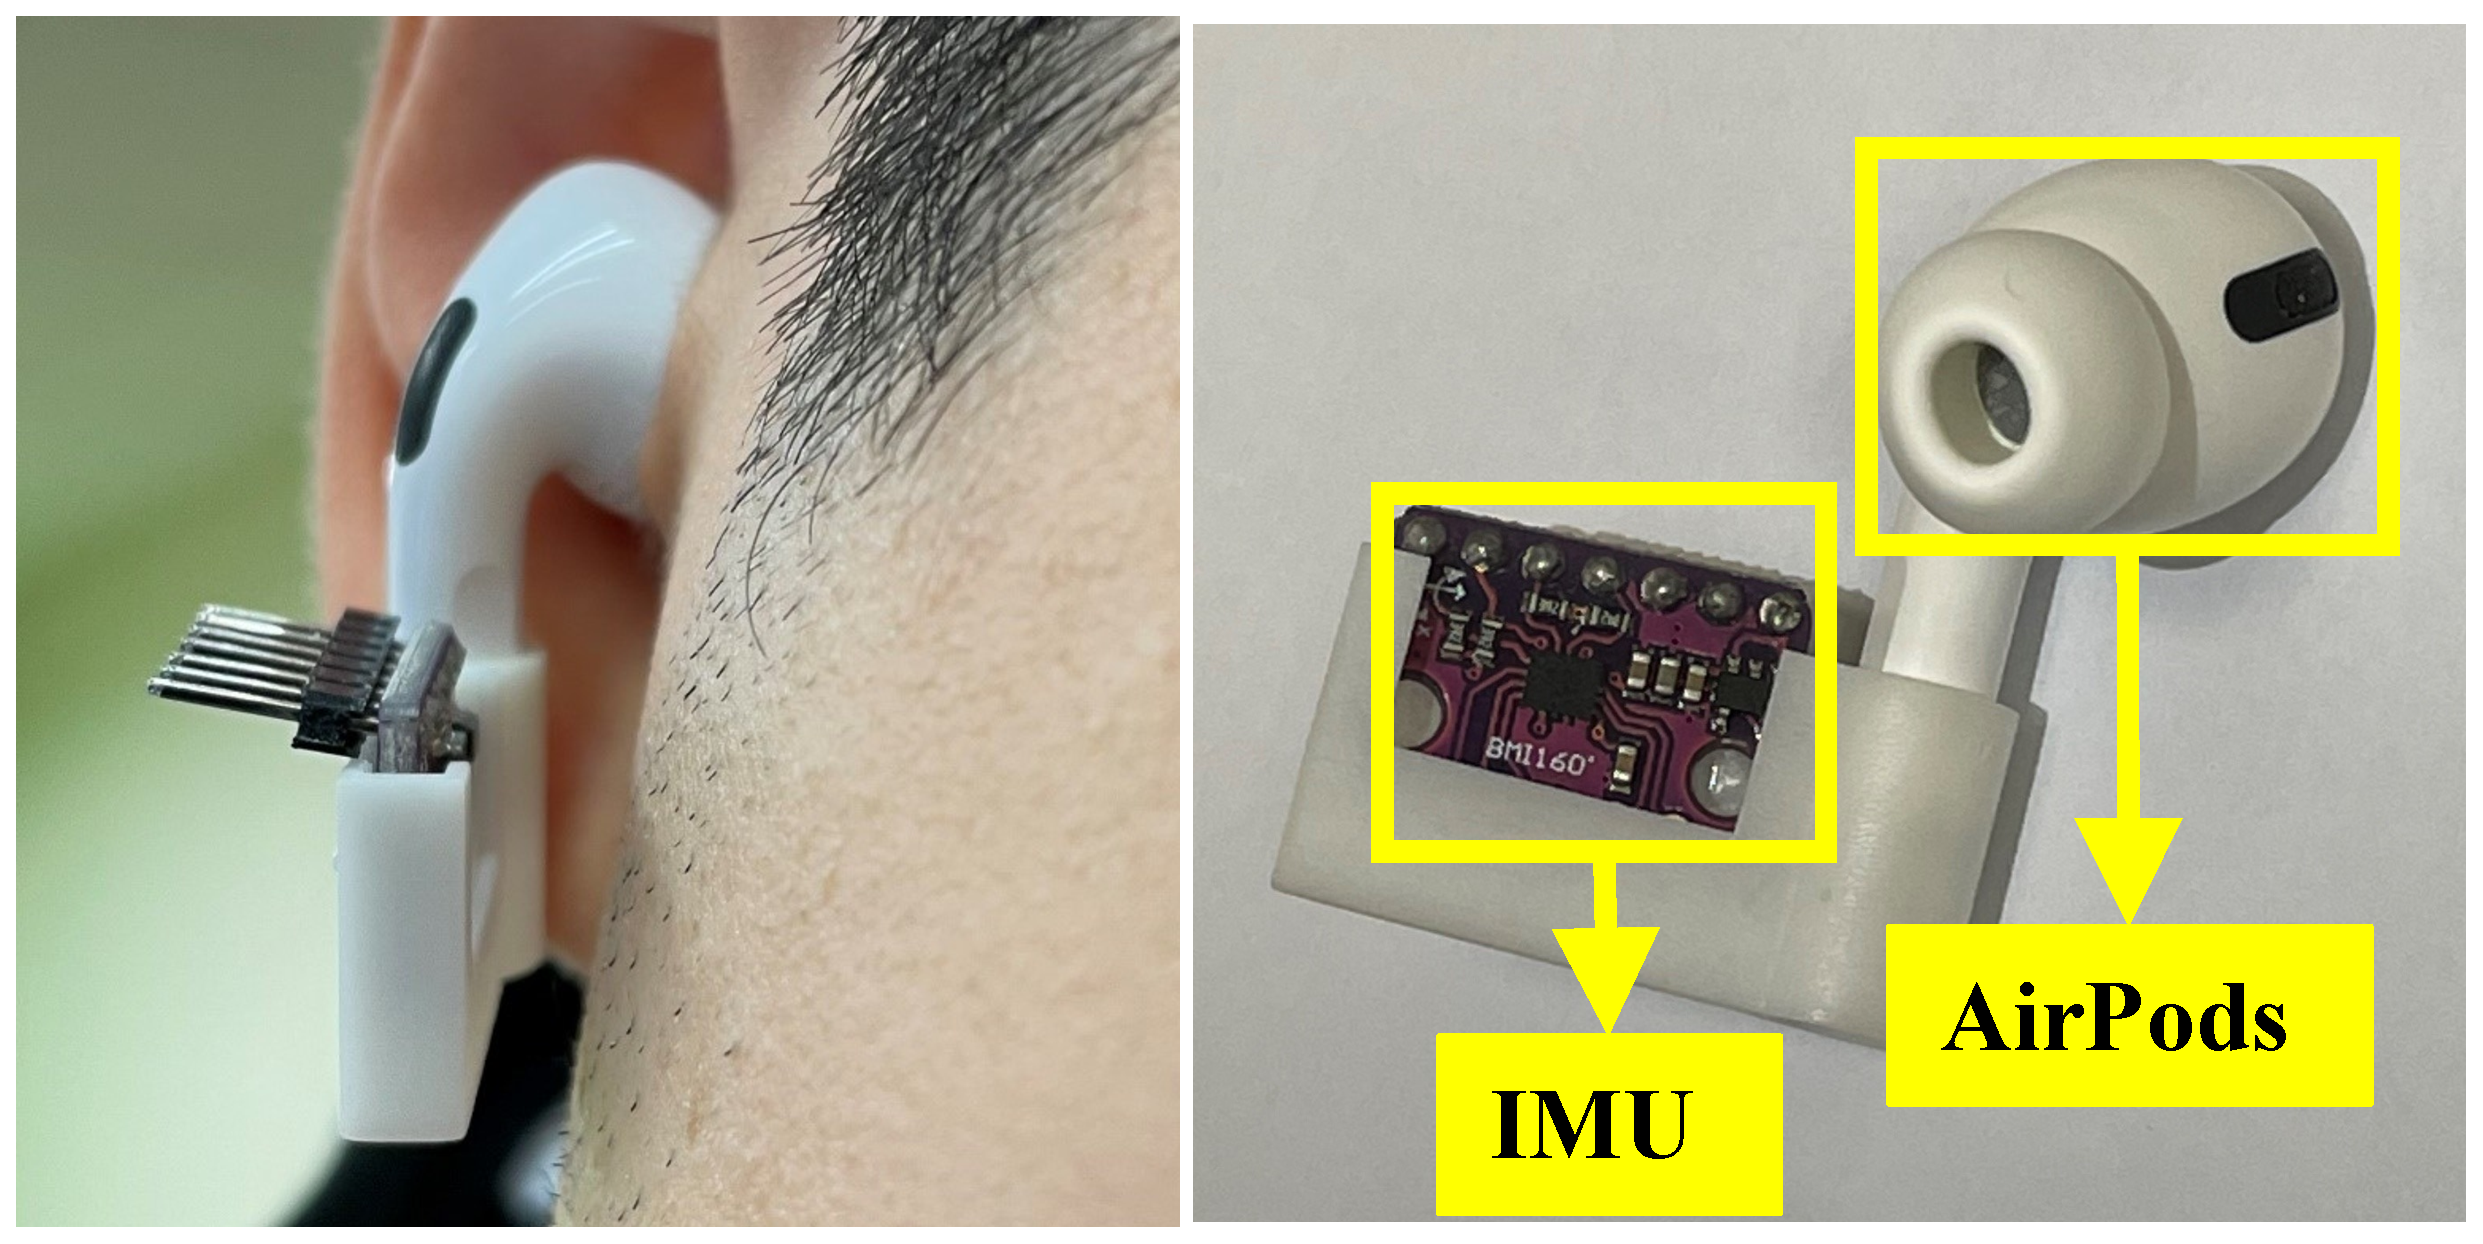
\includegraphics[width=\textwidth]{chapters/vibvoice/figure/earsense.eps}
    \caption{\emph{EarSense} with an Airpods Pro.}
    \label{fig:vibvoice_earsense-head}
  \end{subfigure}
  \begin{subfigure}{0.35\columnwidth}
    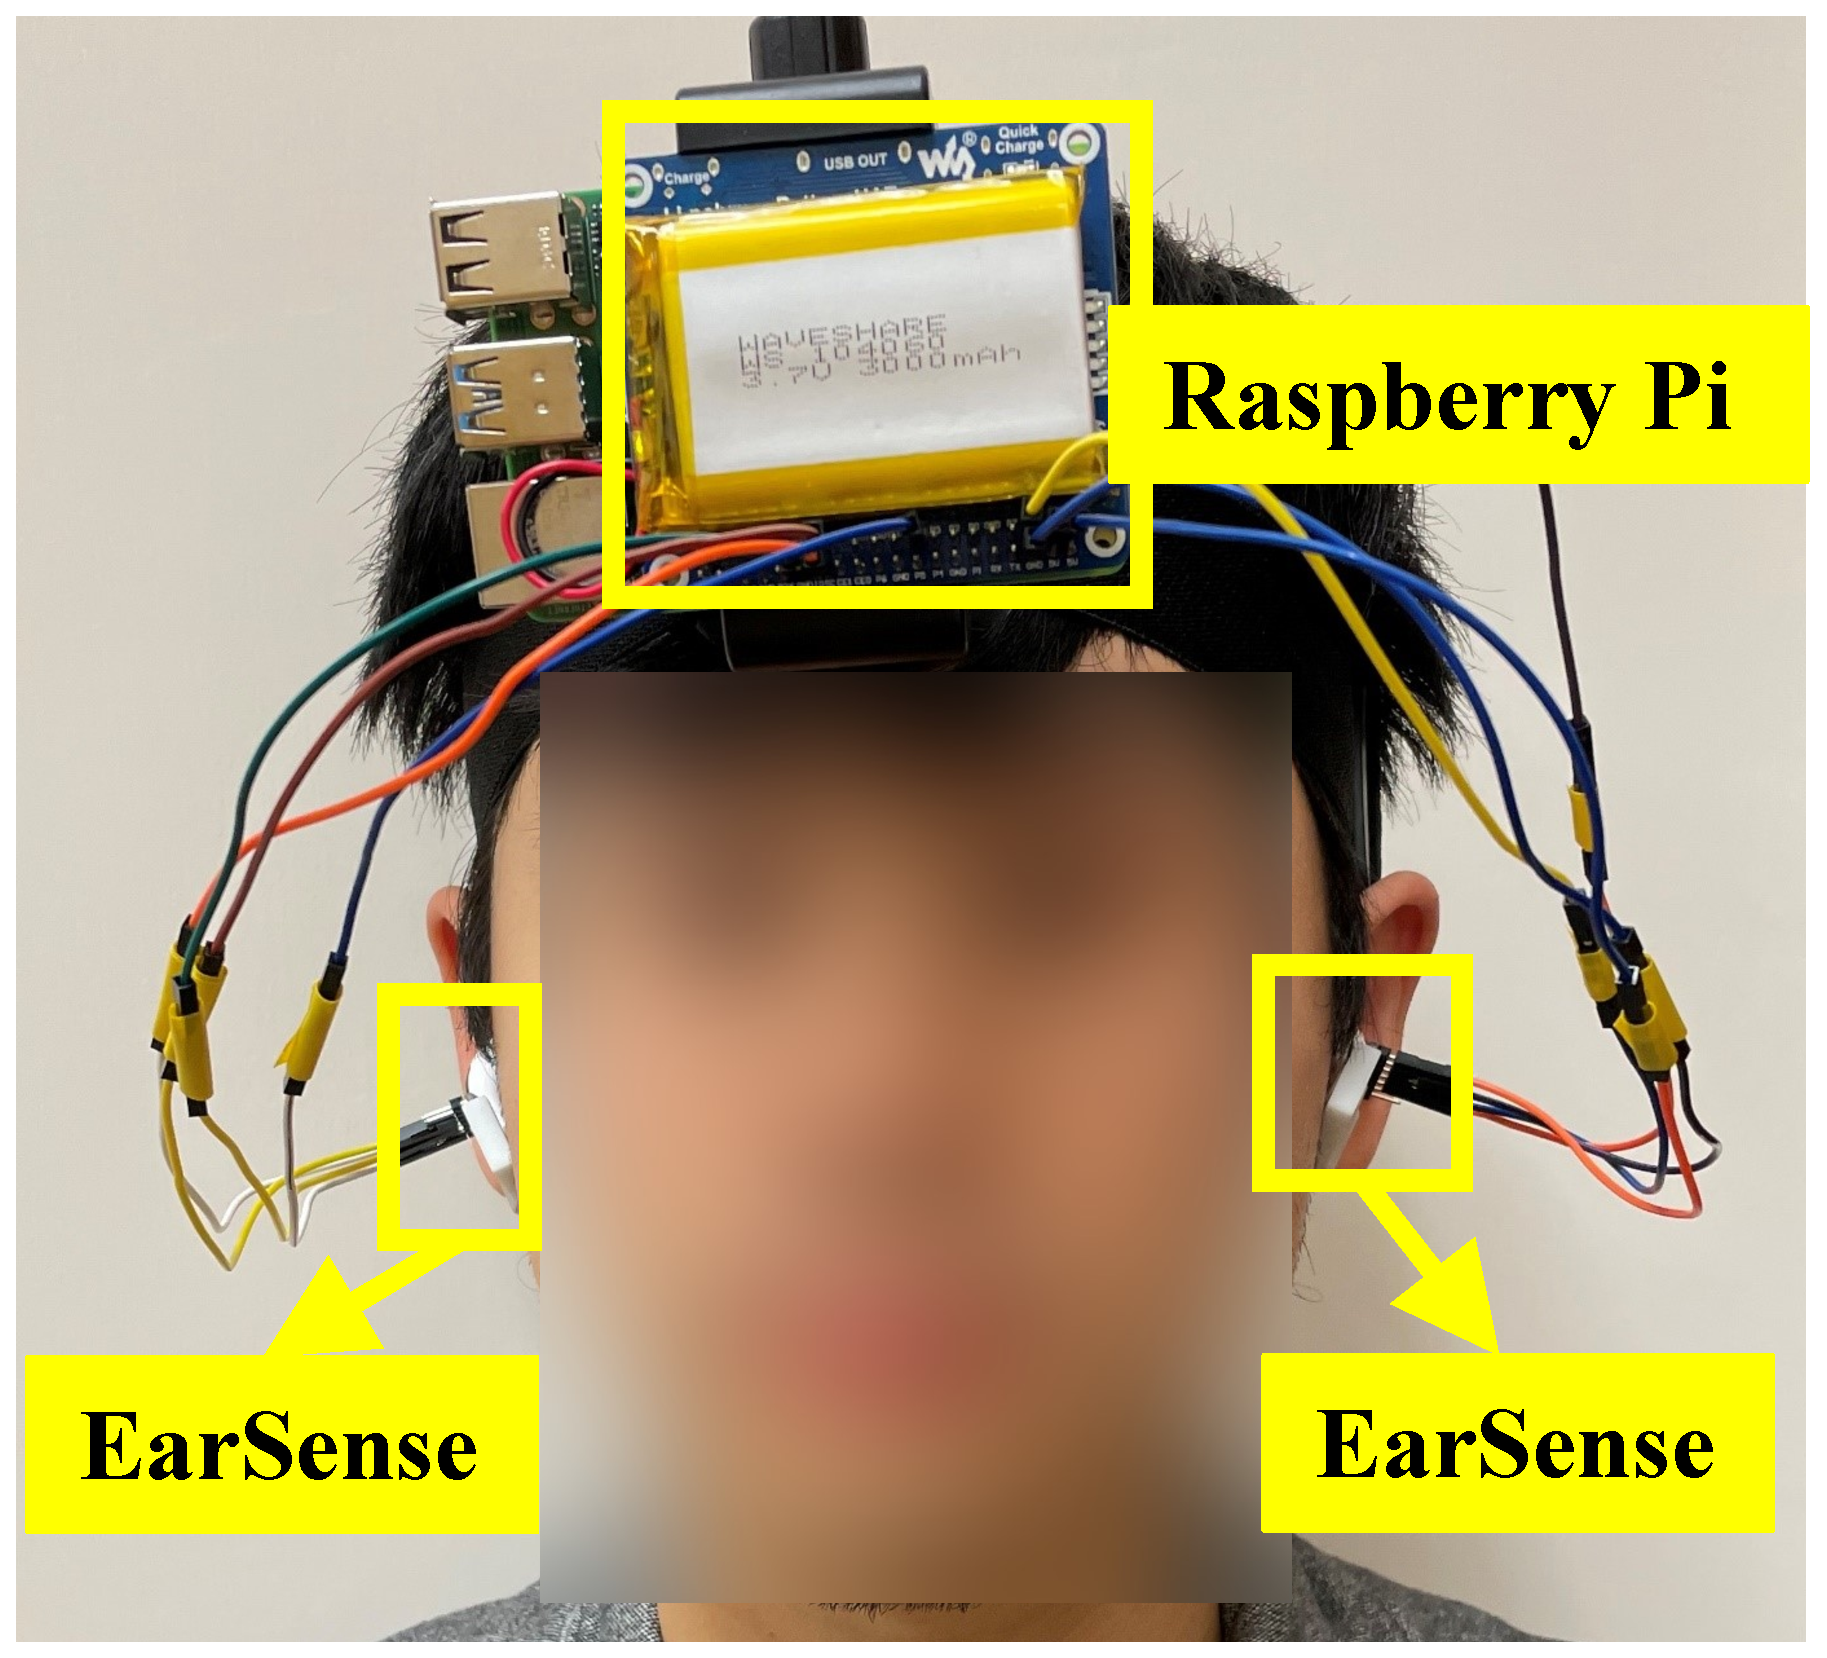
\includegraphics[width=\textwidth]{chapters/vibvoice/figure/people.eps}
    \caption{Test Setup.}
    \label{fig:vibvoice_earsense-people}
  \end{subfigure}
  \caption{\emph{EarSense} is an open-sourced data collector attachable to commercial HMWs for vibration sensing.}
  \label{fig:vibvoice_earsense}
\end{figure}

Fig. \ref{fig:vibvoice_earsense} shows the prototype of \textit{EarSense}  \citep{dataset}, a new open-sourced sensing platform that equips a 3D-printed enclosure with an IMU sensor (i.e., Bosch BMI-160 \citep{Inertial63:online}) inserted. EarSense has a flexible design to make it attachable to any commercial HMW device (e.g., AirPods Pro). EarSense captures the same vibration as the testing HMW and has no direct contact with the user's head (shown in Fig. \ref{fig:vibvoice_earsense-head}).
We connect two EarSenses to a Raspberry Pi (RPi) with a battery for data collection.
Fig. \ref{fig:vibvoice_earsense-people} shows a volunteer wearing the device on the head to avoid excessive vibrations caused by the connecting wires.
A Python script on the RPi controls the EarSense devices through the I2C protocol and stores the data for offline processing.
We only use the three-axis accelerometer provided by the IMU chip because the gyroscope and magnetometer are less related to the vibration.
The default sample rates of the microphone and accelerometer are $16\,\text{kHz}$ and $1.6\,\text{kHz}$, respectively. Since commercial earphones such as AirPods Pro do not support two-channel audio recording through public APIs, EarSense records audio in a mono channel.
We apply L2-Norm to the spectrograms of three-axis acceleration to extract the vibration intensity and avoid the impact of wearing position and user's motion.

\subsection{Measurements of Bone-Conducted Vibrations}
\label{sec:vibvoice_measurement}
We measure the difference between audio and bone-conducted vibrations with EarSense under various settings, i.e., the noises caused by the competing speaker and user motion. In each experiment, we ask a volunteer to wear Apple AirPods Pro with EarSense attached (shown in Fig. \ref{fig:vibvoice_earsense-people}) in a meeting room with the size of $10~\text{m}^2$. 
\begin{figure}
    \begin{subfigure}{0.46\columnwidth}
        \centering
        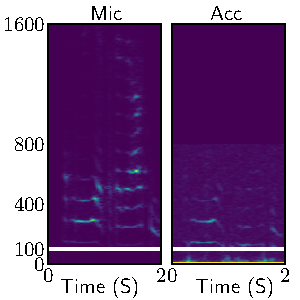
\includegraphics[width=1\textwidth]{chapters/vibvoice/figure/clean.pdf}
        \caption{The user is talking with no noise.}
        \label{fig:vibvoice_nospeaker}
        \end{subfigure}
        \hspace{.5em}
    \begin{subfigure}{0.46\columnwidth}
        \centering
        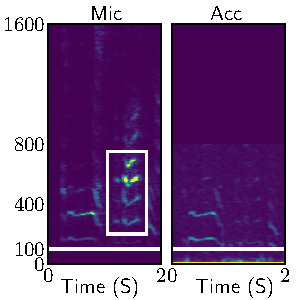
\includegraphics[width=1\textwidth]{chapters/vibvoice/figure/noise.pdf}
        \caption{The user is talking with a competing speaker.}
        \label{fig:vibvoice_speaker}
         \end{subfigure}
    \caption{Impact of the competing speaker.}
    \label{fig:vibvoice_competing-speaker}
\end{figure}

\noindent\textbf{Competing speaker.}
First, we ask the user to sit in the meeting room and speak while a loudspeaker is playing a pre-recording speech one meter from the user as the competing speaker. Note that the competing speaker is one of the most challenging environmental noises for HMWs since its spectrum is similar to the speech's, making it indistinguishable from the noise suppression algorithms. 
We set the volume of the competing speaker to be similar to the user, in which SNR is 3 dB. It is difficult to separate the two sources according to volume since the two speeches are mixed.
Fig. \ref{fig:vibvoice_nospeaker} and Fig. \ref{fig:vibvoice_speaker} show the spectrograms of microphone audio and acceleration when the environment is quiet or contains a competing speaker when the user is talking, respectively.
Note that we only show the spectrogram up to $1.6\,\text{kHz}$ since there is slim energy in the frequency bands higher than $1.6\,\text{kHz}$ of the microphone, and the accelerometer can only sense the signal with a frequency band of $800\,\text{Hz}$.
The spectrograms show that acceleration has lower signal energy than microphone audio since acoustic vibration attenuates during bone conduction, especially for high-frequency vibrations. Compared with the silent environment, the audio spectrogram of microphone audio with a competing speaker shows strong distortions, as highlighted with the white box in Fig. \ref{fig:vibvoice_speaker}. However, the accelerometer spectrograms do not show this phenomenon because the competing speaker cannot produce bone-conducted vibrations.
In summary, the accelerometer receives the user's voice through bone conduction only, excluding environmental sounds over the air, which is ideal for speech enhancement.

\noindent\textbf{User motion.}
We also measure the noises caused by the user's motion. We ask the volunteer to walk while talking. Fig. \ref{fig:vibvoice_walk} shows that walking causes low-frequency noises in the acceleration. The green boxes show the zoom-in result of the signals below $100\,\text{Hz}$. We can observe clear periodic fluctuations in low frequency (i.e., $< 50\,\text{Hz}$), which are caused by the steps of the volunteer.
In summary, the user's motion only affects the acceleration at lower frequencies, which does not affect our speech enhancement.
In addition, we observe slight low-frequency fluctuation in acceleration in Fig. \ref{fig:vibvoice_competing-speaker}, although the volunteer is asked to stand still in this experiment. Since most of the human speech is above $85~\text{Hz}$ \citep{Voicefre75:online}, the removal of audio in low frequency (i.e., the white horizontal lines in Fig. \ref{fig:vibvoice_competing-speaker}) can effectively reduce the interference caused by human motion.

\begin{figure}
\begin{minipage}[t]{0.46\columnwidth}
     \centering
        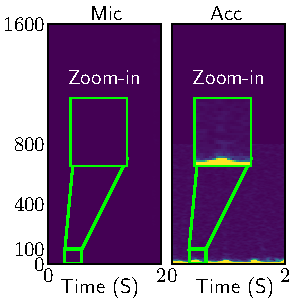
\includegraphics[width=1\textwidth]{chapters/vibvoice/figure/notalk.pdf}
        \caption{Spectrograms of microphone and acceleration when the user is walking.}
        \label{fig:vibvoice_walk}
\end{minipage}
\hfill
   \begin{minipage}[t]{0.48\columnwidth}
     \centering
       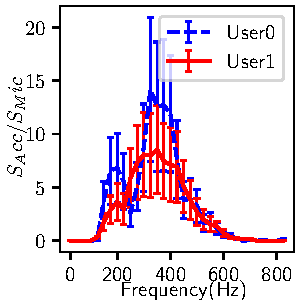
\includegraphics[width=1\textwidth]{chapters/vibvoice/figure/transfer_variance.pdf}
    \caption{Frequency responses of two users' bone-conducted vibrations.}
    %\vspace{-2em}
    \label{fig:vibvoice_bcf}
\end{minipage}
\end{figure}

\noindent\textbf{Frequency Response.}
We further explore the frequency response of bone-conducted vibrations among users. 
Specifically, we measure the frequency response of bone-conducted vibrations as follows: First, we compute the spectrums of audio and vibration data, which is denoted by $S_{Mic}$ and $S_{Acc}$, respectively. Then, we compute the Bone Conduction Function denoted by the frequency response of bone-conducted vibrations by $S_{Acc}/S_{Mic}$ at every frequency band. Fig. \ref{fig:vibvoice_bcf} shows two volunteers' frequency responses, in which the error bars represent the averages and variances.
The acceleration shows higher sensitivity than the microphone within the frequency of $200\text{Hz}\sim500\text{Hz}$, while lower sensitivity at a higher frequency ($>500\text{Hz}$) due to the absorption by the head skull. 
In addition, the frequency response keeps significant similarity among users, indicating the generalization to other users.
Hence, the Bone Conduction Function should consider inter-people diversity and inter-people similarity.

\begin{figure}
\begin{minipage}[t]{0.48\columnwidth}
     \centering
    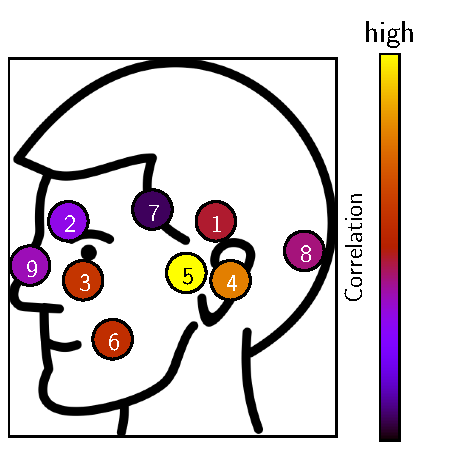
\includegraphics[width=\textwidth]{chapters/vibvoice/figure/correlation.pdf}
    \caption{Intensities of received bone-conducted vibrations on ten locations of the head.}
    \label{fig:vibvoice_head_positison}
\end{minipage}
\hfill
   \begin{minipage}[t]{0.48\columnwidth}
     \centering
    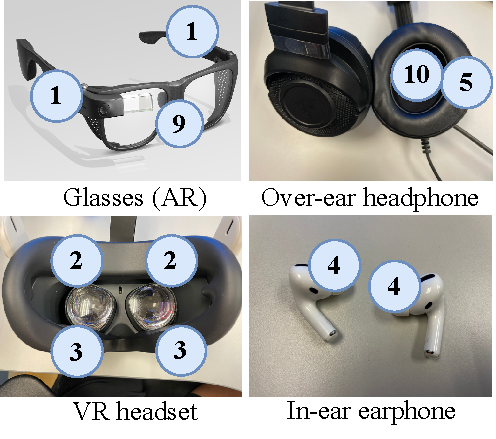
\includegraphics[width=\textwidth]{chapters/vibvoice/figure/devices.pdf}
    \caption{Potential placements on devices.}
    \label{fig:vibvoice_devices}
\end{minipage}
\end{figure}
\noindent\textbf{Locations on the head.}
Bone-conducted vibration exists at various locations on the head. 
As shown in Fig. \ref{fig:vibvoice_head_positison}, we select ten unique locations of interest on the head and measure the intensities of received bone-conducted vibrations. In particular, the nine locations are \#1 \emph{upper ear}, \#2 \emph{eyebrow}, \#3 \emph{cheekbones}, \#4 \emph{ear}, \#5 \emph{temporomandibular joint}, \#6 \emph{cheek}, \#7 \emph{temple}, \#8 \emph{back of the head}, and \#9 \emph{nose}. In addition, we tape EarSense on the interior of the pad of an over-ear headphone, which is denoted as \#10.
Among those positions, some are compatible with commercial HMWs like glasses, headphones, and VR headsets. Fig. \ref{fig:vibvoice_devices} illustrates the corresponding positions on HMWs. The numbers on the HMWs correspond to the locations in Fig. \ref{fig:vibvoice_head_positison}. 
We attach EarSense to the HMWs (when applicable) or on the face for all the following tests. 
We compute Pearson correlation coefficients between the audio and the acceleration on each location and mark the values using a color map in Fig. \ref{fig:vibvoice_head_positison}.
We observe that bone-conducted vibrations exist at most locations of the head. In particular, locations closer to the mouth show higher correlations, indicating a larger possibility of extracting clean speech. 

In summary, our measurements show that bone-conducted vibration has the following characteristics: a) Bone-conducted vibration is robust to environmental voice and only captures the user's speech; b) The user's motion only generates vibrations lower than $85\,\text{Hz}$; c) Bone-conducted vibration has suppressed low and high-frequency audio, which varies across users and within the same user; and d) We can receive audio from multiple locations on the head.



\section{Methodology}
\label{sec:vibvoice_method}
\subsection{Overview of VibVoice}
\label{sec:vibvoice_overview}
\begin{figure*}
  \centering
  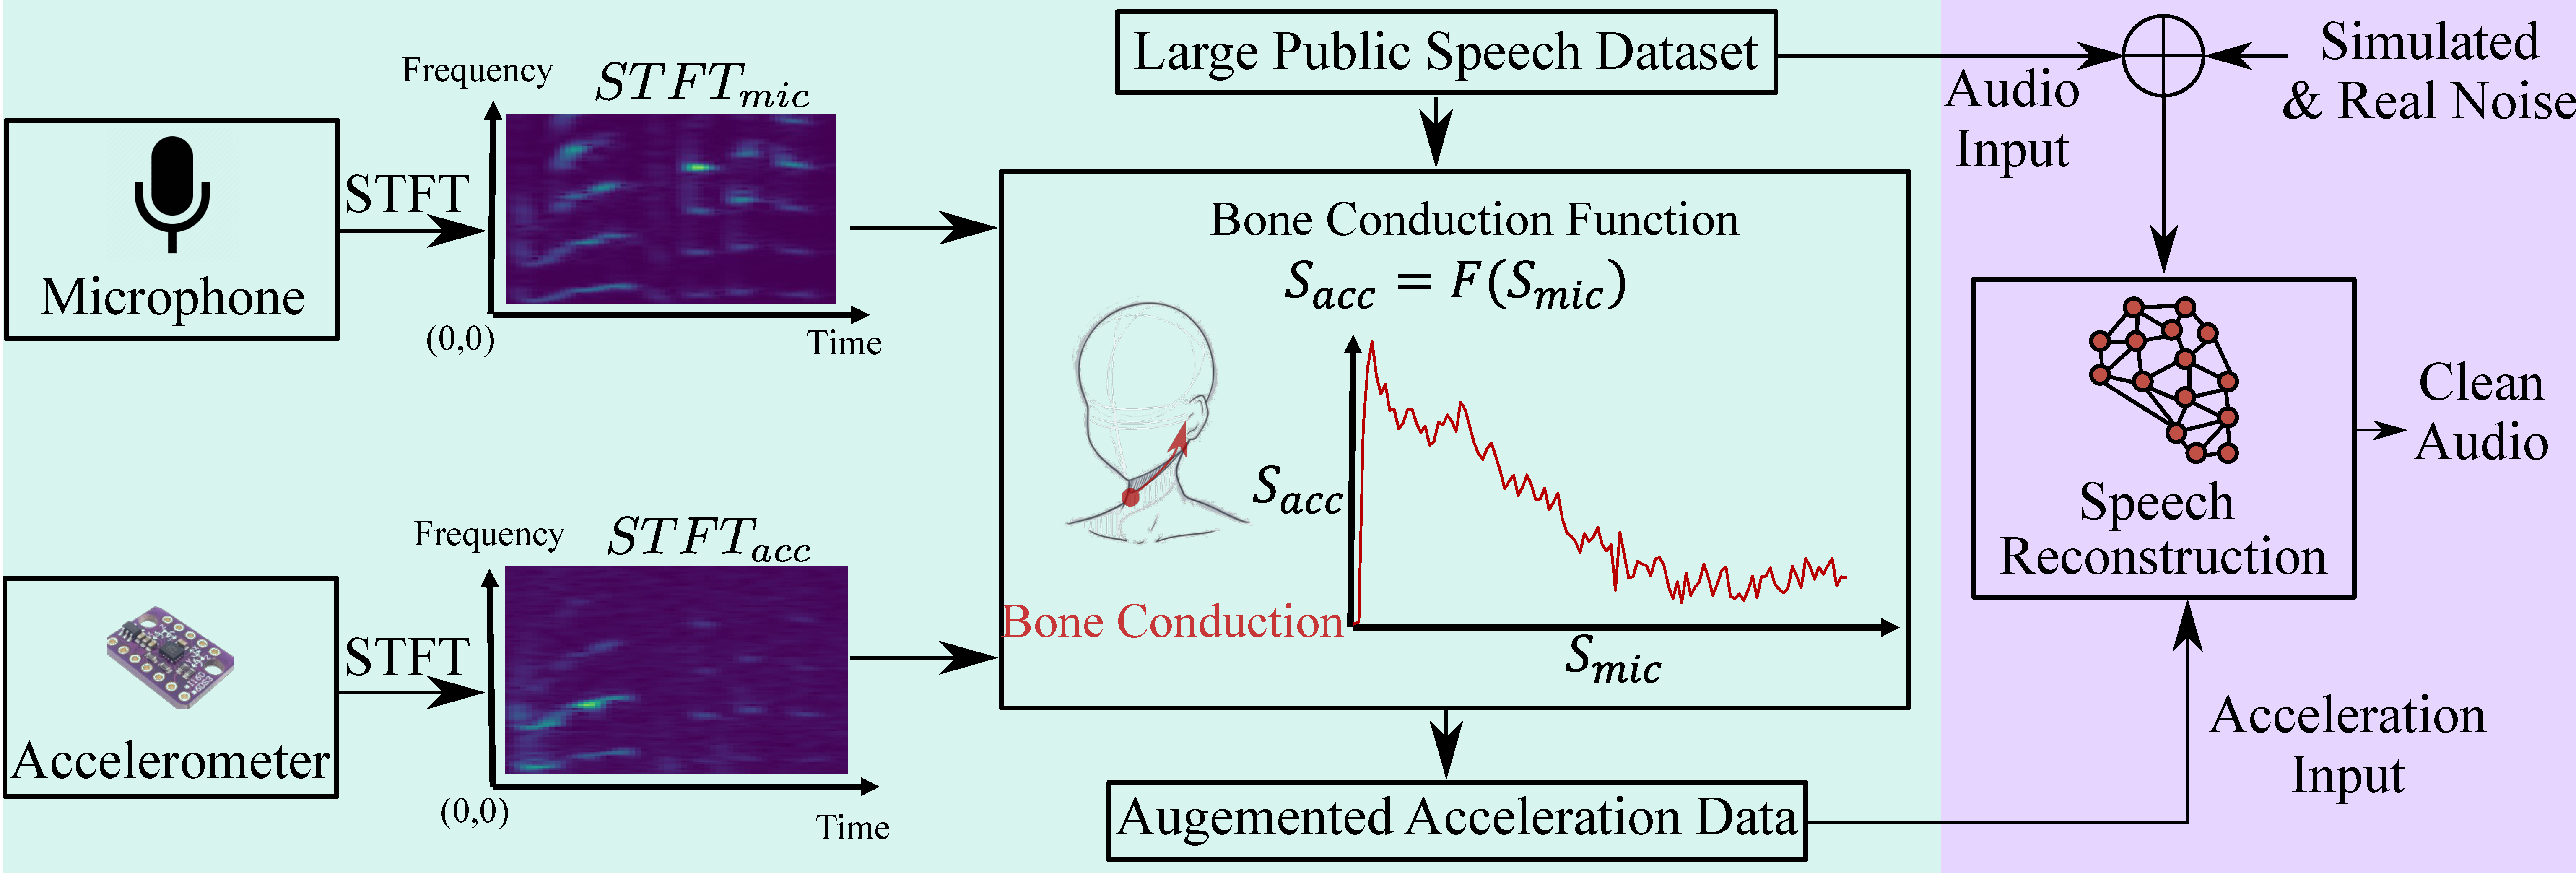
\includegraphics[width=.85\textwidth]{chapters/vibvoice/figure/overview.pdf}
  \caption{The overview of \textit{VibVoice} system. We first augment the acceleration data using a large public speech dataset with estimated Bone Conduction Functions (e.g., the greed box). Then, we train a multi-modal DNN for speech reconstruction (e.g., the purple box).}
  \label{fig:vibvoice_overview}
\end{figure*}
Motivated by our findings in Section. \ref{sec:vibvoice_measurement}, bone-conducted vibration is a promising complementary sensing modality to microphone recording for speech enhancement under environmental noises. 
However, the limited sample rate of HMW's accelerometer and diverse frequency responses of bone-conducted vibration introduce challenges for multi-modal speech enhancement. 
On the other hand, although it is possible to adapt existing audio-only DNN-based speech enhancement models \citep{michelsanti2021overview,sun2021ultrase, zhang2021sensing,liu2021wavoice, ozturk2021radiomic} to take both inputs, there is no large dataset with paired acceleration and audio on HMWs available.

We design \textit{VibVoice}, a speech enhancement system for HMWs that leverages both the microphone recording and the speech information from the bone-conducted vibrations.
Fig. \ref{fig:vibvoice_overview} overviews the design of VibVoice, which contains three components: estimation of Bone Conduction Function, data augmentation, and speech reconstruction network.
% The system overview is shown in Fig. \ref{fig:vibvoice_overview}. 
First, we estimate a set of Bone Conduction Functions using a small paired acceleration-audio dataset collected from volunteers in Section. \ref{sec:vibvoice_function}. 
We note that this estimation does not resort to black-box deep learning approaches, which require a huge amount of training data. Instead, we take advantage of prior knowledge that a frequency response exists between the acceleration and audio spectrograms. 
Then, we augment the acceleration data using the public audio dataset \textit{LibriSpeech} \citep{panayotov2015librispeech} with Bone Conduction Functions in Section. \ref{sec:vibvoice_aug}.
Finally, after generating a large amount of paired acceleration-audio dataset, we train a DNN model which can reconstruct the clean audio from microphone audio and the acceleration data in Section. \ref{sec:vibvoice_network}. 

\subsection{Bone Conduction Function}
\label{sec:vibvoice_bcf}
\subsubsection{Function Formulation}

Measurements in Section. \ref{sec:vibvoice_measurement} show that the acceleration contains acoustic vibrations caused by bone conduction effects. There are two characteristics of acoustic vibrations: a limited sample rate up to $800~\text{Hz}$ and diverse amplitude suppression levels at frequency bands. We model the vibration sensed by the accelerometer as follows: 
\begin{equation}
  s_{acc} = f(s_{mic}) + \epsilon_{acc}=f(s_{speech} + \epsilon_{mic}) + \epsilon_{acc},
  \label{math:transfer_function}
\end{equation}
where $s_{acc}$ and $s_{mic}$ are the raw data captured by the accelerometer and the microphone, respectively; $s_{speech}$ denotes the ground-truth (clean) speech audio; $\epsilon_{acc}$ and $\epsilon_{mic}$ are environmental noises captured by the accelerometer and the microphone, respectively; and $f$ is the Bone Conduction Function.

\subsubsection{Function Estimation}
\label{sec:vibvoice_function}
To estimate the Bone Conduction Function, we recruit volunteers and record a five-minute speech for each person with EarSense and AirPods Pro. The volunteers are asked to read from a daily conversation material \citep{Everyday75:online} in a silent environment. We split paired data into 5-second windows, and each window can contribute one Bone Conduction Function.

First, we compute the spectrograms $STFT_{acc}$ and $STFT_{mic}$ of $s_{acc}$ and $s_{mic}$ for each window using short-time Fourier transform (STFT), respectively.
Then, we apply Otsu's method \citep{otsu1979threshold} to $STFT_{acc}$ and $STFT_{mic}$ for automatic image thresholding, and then discard the bins whose value is lower than a threshold to remove outlier noises.
We note that our thresholding setting can leverage temporal information, which can better diminish the noise than a constant threshold on the frequency or time domains.
Furthermore, we perform the pixel-wise division between $STFT_{acc}$ and $STFT_{mic}$ to obtain a response spectrogram, selecting the lower frequency part of the audio spectrogram to align to the acceleration spectrogram. 
We model the Bone Conduction Function using the Gaussian distribution in the frequency domain since the frequency response (as shown in Fig. \ref{fig:vibvoice_bcf}) has a non-trivial variance due to the complex structure of the head skeleton \citep{chang2016development}. 
In particular, we compute $f=S_{acc}/S_{mic}$ for the corresponding time window in $STFT_{acc}$ and $STFT_{mic}$, respectively. The function $f\sim N(\mu,\sigma^2)$, in which $\mu$ and variance $\sigma$ contribute to the contour and fluctuation of frequency response, respectively.
We measure $\mu$ and $\sigma$ for each time window to construct the parameter pool of Bone Conduction Functions. 

\subsubsection{Data Augmentation with Bone Conduction Functions}
\label{sec:vibvoice_aug}
\begin{figure}
    \centering
    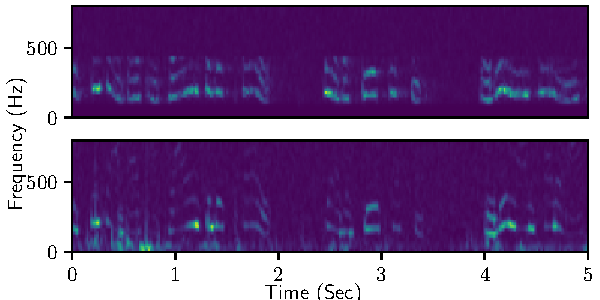
\includegraphics[width=0.35\textwidth]{chapters/vibvoice/figure/synthetic_compare.pdf}
    \caption{Augmented (upper) and real (lower) Acceleration.}
    %\vspace{-1em}
    \label{fig:vibvoice_synthetic_compare}
\end{figure}
We develop a data augmentation approach with Bone Conduction Functions described in Section. \ref{sec:vibvoice_function}.
Note that we cannot apply the inverse Bone Conduction Function to turn the acceleration back to audio due to the significantly limited sample rate of acceleration data. In addition, the frequency band (larger than $500\,\text{Hz}$) has very slim energy, which can cause unreasonable large energy after the inversion.
We utilize these functions to generate acceleration signals using a large-scale audio dataset, i.e., LibriSpeech \citep{panayotov2015librispeech}. 
To be specific, for each audio clip, we first select a Bone Conduction Function (i.e., a list of means and variances over different frequencies) from the pool randomly. 
Then, we restore the frequency response from the Gaussian distribution of given parameters. 
Lastly, we can augment the audio to synthetic acceleration data by directly multiplying the frequency response. 

Fig. \ref{fig:vibvoice_synthetic_compare} shows the spectrograms of augmented acceleration and real acceleration signals, respectively. The augmented spectrogram is close to the real acceleration spectrogram. 
We compute the similarity by calculating the mean of the absolute distance of all pixels in the whole spectrogram and divide it by the largest value of the real acceleration spectrogram. The average error for all volunteers is only 4.5\%, which indicates that our proposed acceleration augmentation is reliable. 

\subsection{Multi-Modal Speech Reconstruction}
\label{sec:vibvoice_network}
Since the sample rate of the microphone is $16\,\text{kHz}$ while the accelerometer is only $1.6\,\text{kHz}$. The reconstruction of high-quality audio from acceleration is an ill-posed task since it requires predicting the lost patterns of the high-frequency band.
Moreover, as we have already generated a large-scale paired acceleration-audio dataset, we can unleash the strong feature extraction capability of DNNs for training. Compared with hand-crafted signal processing approaches, deep learning is robust to diverse inputs. Specifically, we adapt the multi-modal fusion paradigm \citep{sun2021ultrase, zhang2021sensing} and encoder-decoder architecture based on U-net \citep{ronneberger2015u} to build the deep learning model. 
Fig. \ref{fig:vibvoice_CNN} overviews of the DNN design, which is described in detail as follows.


\begin{figure}[tbp]
  \centering
  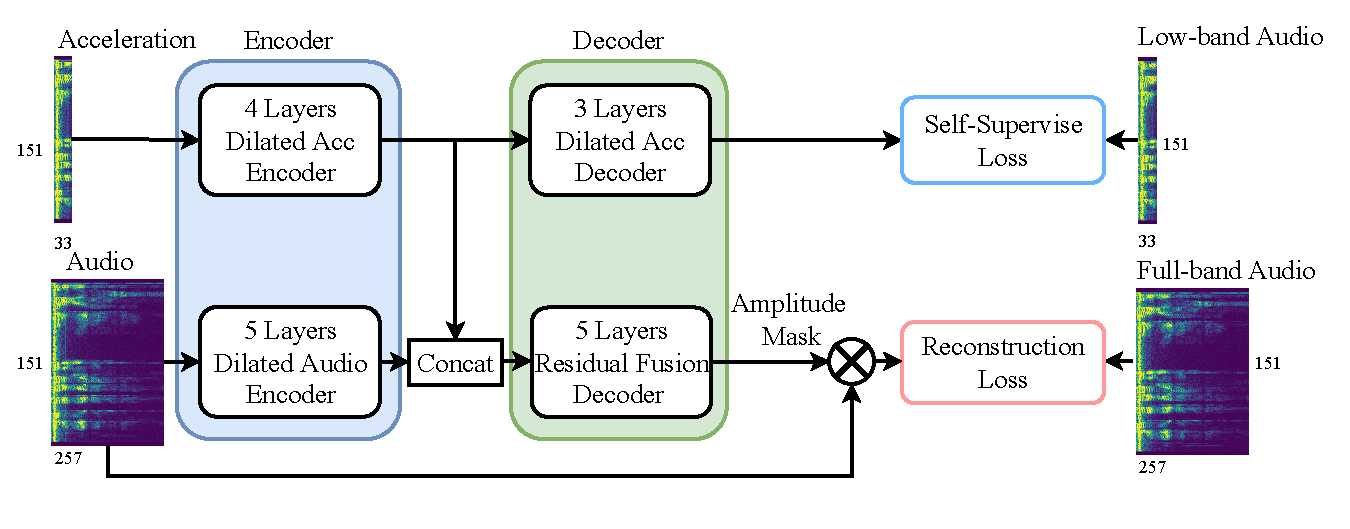
\includegraphics[width=.5\textwidth]{chapters/vibvoice/figure/network.pdf}
  %\vspace{-2em}
  \caption{Overview of our proposed multi-modal network for speech enhancement.}
  \label{fig:vibvoice_CNN}
\end{figure}

\begin{table}[ht!]
\centering
\begin{subtable}[t]{0.5\textwidth}
\centering
\begin{tabular}{lccccccc}\toprule
& \multicolumn{4}{c}{Encoder} & \multicolumn{3}{c}{Decoder}
\\\cmidrule(lr){2-5} \cmidrule(lr){6-8}
Layer & 1 & 2 & 3 & 4 & 1 &2 &3 \\\midrule
Filters &16 &32&64&128 & 64&32 & 16\\ 
Kernel &3 &3&3&3&3&3&3\\ 
Scale &1 &1&0.5&0.5&1&2&2\\
\bottomrule
\end{tabular}
\caption{\label{table1}Acceleration branch.}
\end{subtable}

\begin{subtable}[t]{0.5\textwidth}
\begin{tabular}{lcccccccccc}\toprule
& \multicolumn{5}{c}{Encoder} & \multicolumn{5}{c}{Decoder}
\\\cmidrule(lr){2-6} \cmidrule(lr){7-11}
Layer  & 1 & 2 & 3 & 4 & 5 & 1 &2 &3 &4 & 5  \\\midrule
Filters &16 &32&64&128&256& 128 &64 & 32 & 16 & 1 \\ 
Kernel &3 &5&5&5&5&5& 5 &5 & 5 &3\\ 
Scale &0.5 & 0.5 &0.5 &0.5 & 0.5 & 2 &2 & 2 & 2 & 2\\
\bottomrule
\end{tabular}
\caption{\label{table2}Audio branch.}
\end{subtable}
\caption{{The design of DNN for multi-modal speech reconstruction.}}
\end{table}

\subsubsection{\textbf{Architecture}}
Table \ref{table1} and \ref{table2} show the hyperparameters of our multi-modal neural network of the acceleration and audio branches, respectively. The details are illustrated as follows.

\noindent\textbf{Encoder}.
We use two convolutional networks (CNNs) to encode the high-level features from the two modalities, respectively. Then, we concatenate the features from two encoders along the channel dimension. We stack basic blocks to construct the encoder, where each block consists of a 2D convolutional layer, batch normalization, ReLU activation, and max-pooling. We also design a residual shortcut of the block input before the last deconvolution layer to expedite the training. The filters increase when the layer gets deeper to extract more diverse features. To increase the reception field to capture the harmonic pattern of the whole spectrogram, we use dilated convolution rather than the conventional one.
Since the sample rate of audio data (i.e., $16\,\text{kHz}$) is ten times higher than that of the acceleration data ($1.6\,\text{kHz}$), the size of the audio spectrogram on the frequency axis is also ten times larger. We note that the feature maps from the two modalities should have the same shape at the end of the encoders. Therefore, we discard the parts of the audio spectrogram whose frequency is higher than $6.4\,\text{kHz}$, making the remaining audio frequency band exactly eight times larger than the acceleration data (i.e., $0.8\,\text{kHz}$). In addition, the audio subnet (i.e., encoder) has three more down-sample operations than the acceleration branch to make the output sizes of the two modalities' features consistent. 

\noindent\textbf{Decoder}.
We design two decoders: a fusion decoder and an auxiliary decoder. The decoder has the same design of blocks as the encoder, but the stacked blocks have a decreasing number of filters but increasing sizes of the output tensor. 
The fusion decoder receives both modalities' features via a concatenation and outputs a spectrogram mask. To obtain the constructed clean spectrogram, this mask will be overlaid on the original noisy audio spectrograms by element-wise multiplication. 
The auxiliary decoder only receives the feature of the accelerometer and predicts the low-frequency part of clean audio. The self-supervised loss can prevent the acceleration encoder from being dominated by the audio input, given that the noisy input audio is similar to the clean audio to acceleration by nature (i.e., both are audio).

\subsubsection{\textbf{Waveform reconstruction}}
After obtaining the enhanced spectrogram from the multi-modal decoder, the last step is converting the spectrogram to the waveform using inverse short-time Fourier transform (ISTFT). The DNN of VibVoice only reconstructs the magnitude of the spectrogram. Since the phase of the speech spectrogram is hardly predictable, we use the same phase of the noisy audio signal for the output. Our insight is that although the audio phase can be polluted in a noisy environment, our reconstructed magnitude can attenuate the unwanted time-frequency pixels in spectrograms, which restricts the interference of the noisy phase. Although several works \citep{sun2021ultrase,zhang2021sensing} try to estimate the clean phase by a subnet or a pre-defined algorithm, our tests show that the predicted phase is unstable, and their improvements are marginal and computationally expensive.

\subsubsection{\textbf{Model Training}}
\label{sec:vibvoice_training}
We generate a pool of Bone Conduction Functions by performing cubic interpolation on existing functions from our dataset. We use Gaussian distribution to alleviate our model's overfitting and improve the generalizability among users. In addition, we augment the data with Gaussian distribution based on each frequency band to preserve the low-pass features.
Thus, the limited Bone Conduction Functions can augment a large acceleration-audio dataset from an existing public dataset with diverse features. This dataset can extract the basic features of multiple modalities, but it is not enough for deployment because of the difference between the target user and our pool of Bone Conduction Functions. 
Therefore, we collected another acceleration-audio paired dataset from a different group of volunteers to train the model, which is also used to evaluate VibVoice's performance. 
Note that VibVoice does not require any data from the target user either during the Bond Conduction Function estimation or model training.
All evaluations adopt leave-one-out validation. We pick one user as the testing dataset, while the others are regarded as the training dataset. 

Although the training of VibVoice does not require any data from the target user, one-shot data from the target domain can further improve the overall performance. This data collection can share the recorded data during the setup of HMWs, e.g., the personalized model for calling voice assistants, which incurs no extra overhead to the user. In addition, VibVoice can record data when the user is speaking in a quiet environment. As the data collection doesn't require specific content, our system can unobtrusively record user-specific data during the long-time usage of HMWs and improve the performance of the target user continuously. 

The fusion decoder uses the STFT Loss \citep{defossez2020real}. We use $y$ and $\hat{y}$ to represent the clean and enhanced signals. The STFT loss can be denoted as follows: 
\begin{align} 
\label{math:stft_loss}
\begin{split}
    L_{stft}(y, \hat{y}) &= L_{sc}(y, \hat{y}) + L_{mag}(y, \hat{y}),
    \\
    L_{sc}(y, \hat{y}) &= \frac{||STFT(y)| - |STFT(\hat{y})||_{F}}{||STFT(y)||_{F}},
    \\
    L_{mag}(y, \hat{y}) &= \frac{1}{T}|log|STFT(y)| - log|STFT(\hat{y})||_{1},
\end{split}
\end{align} 
where $L_{sc}$ refers to convergence
(sc) loss and $L_{mag}$ refers to the magnitude (mag) loss.
We use Mean Square Error (MSE) as the training loss for the auxiliary decoder. The fusion decoder and auxiliary decoder targets are full-band clean spectrogram and lower-band clean spectrogram, respectively. The final loss is formulated as follows: 
\begin{align} 
\label{math:overall_loss}
\begin{split}
    L(y, \hat{y}) &= L_{stft}(y, \hat{y}) + |y_{lowband} - \hat{y}_{lowband}|_{2} \times \lambda,
\end{split}
\end{align}
which is the joint loss function that covers both fusion and auxiliary decoder. We set $\lambda$ to 0.05 to balance the scales of two losses.


\section{Evaluation} \label{sec:vibvoice_evaluation}

\subsection{Experiment Setup} \label{sec:vibvoice_experiment}
We use EarSense introduced in Section. \ref{sec:vibvoice_EarSense} to collect audio and acceleration signals simultaneously\footnote{The experiments that involve human subjects have been approved by the IRB of the authors' institution (CUHK-SBRE-21-0570).}. The volunteers are asked to wear EarSense and speak in a meeting room with the size of $10~\text{m}^2$. The reading material is selected from daily English conversations \citep{Everyday75:online}. Each volunteer reads the material for 30 seconds and repeats it 20 times, generating ten minutes of data. For data augmentation, we recruit eight volunteers to generate a pool of Bone Conduction Functions and use it to augment 100 hours of data from LibriSpeech \citep{panayotov2015librispeech}. 
In addition, we recruit another 15 volunteers for training and testing. For each experiment, we adopt the leave-one-out validation, i.e., training the model for each user with the dataset except that user. The volume of our collected speech is between 60dB to 70dB, which is the same as regular conversations \citep{WhatNois20:online}.
To test VibVoice's robustness to diverse noises, we use three categories of noises with balanced possibility, including environmental noises (50 classes) \citep{piczak2015dataset}, competing speakers from another subset of LibriSpeech \citep{panayotov2015librispeech}, and 20 songs with languages of English, Mandarin, and Japanese. We apply a random room impulse response from dataset \citep{ko2017study}, containing point-source noises, real isotropic noises, and simulated the noises of 600 rooms.
We implement VibVoice using PyTorch and train it on a PC with an Intel i9-12900K CPU and two Nvidia RTX 3090 GPUs. 
The model is trained with a step learning rate scheduler with a learning rate of 0.001 and an Adam optimizer. The epoch number is 30.
The length of the STFT window and the overlap for the audio are 640 and 320, while 64 and 32 are for the acceleration. We open-source the implementation and data in \citep{dataset}.

\subsection{Baseline}
We deploy two baselines, i.e., FullSubNet (FSN) \citep{hao2021fullsubnet} and SEANet (SN) \citep{tagliasacchi2020seanet}.
FSN and SN are two state-of-the-art speech enhancement approaches using audio-only and audio-acceleration inputs, respectively.
We train SN using our dataset since the one used in its paper is not available to the public. Specifically, we train SN using acceleration data with a sample rate of 1.6kHz to ensure it is the same as VibVoice. Note that SN indicates that it supports acceleration data with a wide range of sample rates.

\subsection{Evaluation Metric}\label{metric}
We use three evaluation metrics, i.e., Perceptual Evaluation of Speech Quality (PESQ), Signal Noise Ratio (SNR), and Log-Spectral Distance (LSD), which are described as follows:

%\vspace{0.5em}
\noindent\textit{Perceptual Evaluation of Speech Quality (PESQ)}
is a popular test standard for automatically assessing the user experience of speech quality, defined in P.862 standard by International Telecommunication Union \citep{rix2001perceptual}. The results generated by PESQ represent the opinion scores that range from 1 (bad) to 5 (excellent). We use the wide-band version to evaluate the full-band speech quality in the evaluations.

%\vspace{0.5em}
\noindent\textit{Signal Noise Ratio (SNR)}
is a metric widely used in signal processing that can be measured as follows:
$SNR(x, y) = 10*log_{10}(\frac{y}{x-y})^2$, where $x$ and $y$ denote the estimated and clean audio, respectively.
SNR compares the desired signal and the deviation. A higher SNR value means better audio quality. We use the scale-invariant SNR in the implementation to reduce the impact of scale.

%\vspace{0.5em}
\noindent\textit{Log-Spectral Distance (LSD)}
measures the quality of frequencies between the reconstructed audio and the ground truth audio with: 
$LSD(x, y)= \frac{1}{L} \sum_{l=1}^{L} \sqrt{\frac{1}{K}\sum_{k=1}^{K}(X(l,k) - \hat{X}(l,k))^2}$,
where $l$ and $k$ denote the time and frequency index of the spectrogram, respectively; $X = log(|STFT(y)|^2)$, and $\hat{X} = log(|STFT(x)|^2)$. A higher LSD value means lower audio quality.

\subsection{Overall Performance}
\label{sec:vibvoice_overall_eval}
We investigate VibVoice's performance by mixing clean speech with noise audio randomly picked from the noise dataset. We set the SNR of the noisy data ranges from 0dB to 20dB, with an average of 10dB, which covers a wide spectrum of noise levels.

%\vspace{0.5em}
\noindent\textbf{Target user calibration}.
VibVoice can work out of the box, while data from the target user can further improve performance. Fig. \ref{fig:vibvoice_noise_duration} shows the performance of VibVoice and the two baselines with different amounts of data from the target user, in which zero means no target-user data is used during the training. The results show that longer target-user data can improve performance for all approaches, and VibVoice performs better than baselines with the same amount of calibration data. The calibration data can be collected continuously during usage without the user’s inputs/operations (c.f., Section \ref{sec:vibvoice_training}).
VibVoice achieves the best perceptive performance according to PESQ and the best-reconstructed spectrogram according to LSD. VibVoice and FSN have similar SNR results since they output similar signals in the time domain compared to the clean one. 

%\vspace{0.5em}
\noindent\textbf{Noise type}.
We evaluate the impact of different types of noises in Fig. \ref{fig:vibvoice_noise_type}, i.e., environmental noises, competing speakers, and music. The result shows that VibVoice performs better under all noises and metrics except for the SNR with music noise. This is because the complex and dynamic spectrum of the user's speech and music's vocals introduce minor fluctuations in high frequencies, reflecting large fluctuations in SNR.

%\vspace{0.5em}
\noindent\textbf{Noise level}.
We test VibVoice's performance under noise levels of low (10 dB), medium (5 dB), and high (0 dB with only speech noise). The results in Fig. \ref{fig:vibvoice_noise_level} show that VibVoice has better performance improvements, especially when the noise is challenging, i.e., 21$\%$ improvement on PESQ and 26$\%$ improvement on SNR. This is because the acceleration can more robustly identify the target speech, whereas the audio-only solution is difficult to differentiate sound with a similar pattern (e.g., strong speech noise).

%\vspace{0.5em}
\noindent\textbf{Noise source}.
We evaluate the impact of different numbers of noise sources by repeatedly mixing clean audio with random audio clips. Fig. \ref{fig:vibvoice_noise_number} shows that VibVoice's performance degrades as the number of noise sources increases but still outperforms all the baselines.

%\vspace{0.5em}
\noindent\textbf{Temporal stability}.
We further examine how VibVoice performs for the same user over time. Note that the offset of sensor placement and minor changes in speech can cause a slight change. We collect ten-minute data from three volunteers twice, six months apart. 
The results show that VibVoice changes only slightly over time, from 2.6 to 2.5 for PESQ, 15.7 to 15.5 for SNR, and 4.3 to 4.6 for LSD. VibVoice also outperforms FSN, whose performance is 2.1 for PESQ, 15.2 for SNR, and 11 for LSD.
The results affirm that VibVoice is robust to temporal changes.

%\vspace{0.5em}
\noindent\textbf{Airway blockage}.
The blockage of air transmission caused by personal protective equipment like facial masks can significantly suppress the user's speech volume. 
We ask three volunteers to test VibVoice by speaking the same content with and without facial masks.
The result shows that VibVoice's performance only degrades by 0.05 ($< 2\%$) for PESQ, 0.4 ($<3\%$) for SNR, and 0.1 ($<3\%$) for LSD when the subject wears the mask. 
VibVoice gets a more significant margin than FSN, whose performance is  2.15 for PESQ, 13.8 for SNR, and 10 for LSD. 
This aligns with our expectation since VibVoice uses bone-conducted vibration that is not affected by air transmission.

%\vspace{0.5em}
\noindent\textbf{Variances among users}.
Speech and bone-conducted vibration can differ across users due to vocal features, head skull shapes, body fat, etc.
Fig. \ref{fig:vibvoice_per_user} shows the performance of VibVoice across 15 users. VibVoice shows stable and significantly better performance in PESQ compared to baseline and comparable performance in SNR.

%\vspace{0.5em}
\noindent\textbf{Sensing location}.
We test VibVoice when EarSense is placed in ten locations on the head as defined in Fig. \ref{fig:vibvoice_head_positison}, validating VibVoice's effectiveness for different HMW devices.
The bars in Fig. \ref{fig:vibvoice_locations} show VibVoice's performance at each location. The red line represents the performance of the baseline at \#4 \emph{ear}. 
The results show that VibVoice achieves satisfactory performance at all locations in PESQ.
Note that locations like \#1 \emph{upper ear}, \#2 \emph{eyebrow}, \#5 \emph{temporomandibular joint}, \#7 \emph{temple}, and \#10 \emph{interior of the pad of the headphone} show similar or slightly lower SNR than the baseline, which is because the vibration intensity is slim due to their far distance to the audio source.

%\vspace{0.5em}
\noindent\textbf{Data augmentation effectiveness}.
We evaluate how VibVoice's data augmentation reduces the amount of paired training data needed. We compare the performance of training VibVoice from a) paired data of 18 to 180 hours and b) data augmented from three hours of paired data. The dataset \citep{wang2022fusing} is a large-scale Chinese acceleration and audio dataset collected by earphones, and the bandwidth of acceleration is around 5kHz. The results in Fig. \ref{fig:vibvoice_data_augmentation} show that VibVoice with data augmentation can achieve better performance with $\sim24\times$ less paired data.

%\vspace{0.5em}
\noindent\textbf{Summary}.
VibVoice outperforms FSN and SN by up to $21\%$ for PESQ when the noise volume is low, where the PESQ values for VibVoice and FSN are 2.7 and 2.21, respectively. VibVoice improves SNR by up to $26\%$ when the noise is high-volume speech, where the SNR values of VibVoice and FSN are 2.0 and 1.6, respectively. VibVoice also improves LSD by 50$\sim$80$\%$ under most evaluated factors, which indicates the effectiveness of the multimodal design and data augmentation. In some cases, VibVoice has slightly lower SNR because the user's speech and music vocals can have similar spectra. LSD evaluates the full frequency band without such preference, so VibVoice shows a larger margin on this metric.
We further evaluate the perception of real users through a user study in Section. \ref{sec:vibvoice_user-study}.


Compared with the strong baseline FSN, VibVoice achieves good performance in various cases. 
Compared with the multimodal baseline SN, VibVoice performs better because SN has limited capacity to recover speech information from low-rate acceleration. The data augmentation in SN also does not consider user-specific bone-conduction effects, while VibVoice incorporates measurements of bone-conduction transfer characteristics and target-user features.


\begin{figure}
    \begin{subfigure}{0.32\columnwidth}
        \centering
        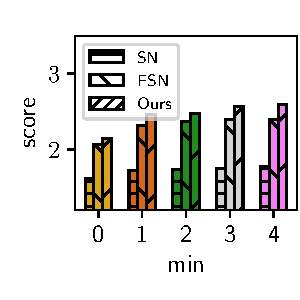
\includegraphics[width=1\textwidth]{chapters/vibvoice/figure/noise_enrollment_0.pdf}
        %\vspace{-1.99em}
        \caption{PESQ.}
        \label{fig:vibvoice_noise_duration_0}
        \end{subfigure}
    \begin{subfigure}{0.32\columnwidth}
        \centering
        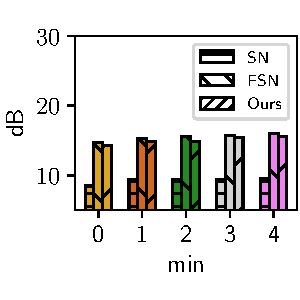
\includegraphics[width=1\textwidth]{chapters/vibvoice/figure/noise_enrollment_1.pdf}
        %\vspace{-1.99em}
        \caption{SNR.}
        \label{fig:vibvoice_noise_duration_1}
         \end{subfigure}
    \begin{subfigure}{0.32\columnwidth}
        \centering
        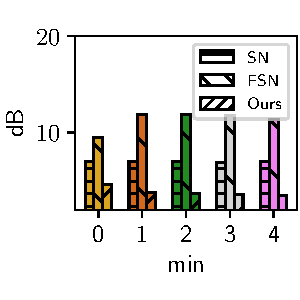
\includegraphics[width=1\textwidth]{chapters/vibvoice/figure/noise_enrollment_2.pdf}
        %\vspace{-1.99em}
        \caption{LSD.}
        \label{fig:vibvoice_noise_duration_2}
         \end{subfigure}
    %\vspace{-1em}
    \caption{Impact of calibration time.}
    \label{fig:vibvoice_noise_duration}
    %\vspace{-1em}
\end{figure}

\begin{figure}
     %\vspace{-0.5em}
    \begin{subfigure}{0.32\columnwidth}
        \centering
        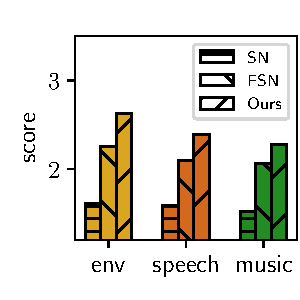
\includegraphics[width=1\textwidth]{chapters/vibvoice/figure/noise_type_0.pdf}
        %\vspace{-1.99em}
        \caption{PESQ.}
        \label{fig:vibvoice_noise_type_0}
        \end{subfigure}
    \begin{subfigure}{0.32\columnwidth}
        \centering
        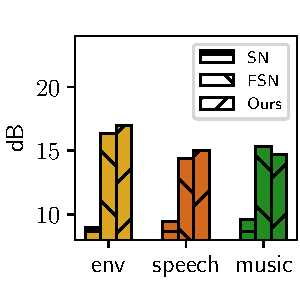
\includegraphics[width=1\textwidth]{chapters/vibvoice/figure/noise_type_1.pdf}
        %\vspace{-1.99em}
        \caption{SNR.}
        \label{fig:vibvoice_noise_type_1}
         \end{subfigure}
    \begin{subfigure}{0.32\columnwidth}
        \centering
        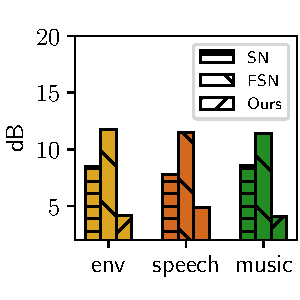
\includegraphics[width=1\textwidth]{chapters/vibvoice/figure/noise_type_2.pdf}
        %\vspace{-1.99em}
        \caption{LSD.}
        \label{fig:vibvoice_noise_type_2}
         \end{subfigure}
    %\vspace{-1em}
    \caption{Impact of noise types.}
    \label{fig:vibvoice_noise_type}
    %\vspace{-1em}
\end{figure}

\begin{figure}
    %\vspace{-0.5em}
    \begin{subfigure}{0.32\columnwidth}
        \centering
        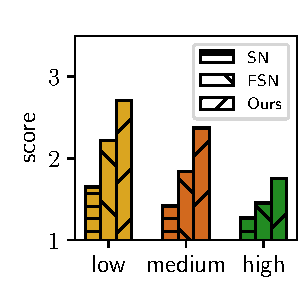
\includegraphics[width=1\textwidth]{chapters/vibvoice/figure/noise_level_0.pdf}
        %\vspace{-1.99em}
        \caption{PESQ.}
        \label{fig:vibvoice_noise_level_0}
        \end{subfigure}
    \begin{subfigure}{0.32\columnwidth}
        \centering
        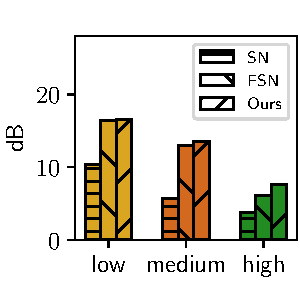
\includegraphics[width=1\textwidth]{chapters/vibvoice/figure/noise_level_1.pdf}
        %\vspace{-1.99em}
        \caption{SNR.}
        \label{fig:vibvoice_noise_level_1}
         \end{subfigure}
    \begin{subfigure}{0.32\columnwidth}
        \centering
        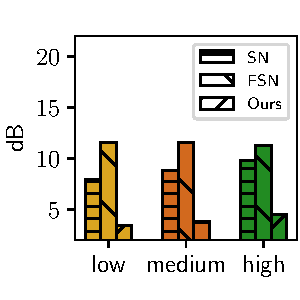
\includegraphics[width=1\textwidth]{chapters/vibvoice/figure/noise_level_2.pdf}
        %\vspace{-1.99em}
        \caption{LSD.}
        \label{fig:vibvoice_noise_level_2}
         \end{subfigure}
    %\vspace{-1em}
    \caption{Impact of noise levels.}
    \label{fig:vibvoice_noise_level}
    %\vspace{-1em}
\end{figure}

\begin{figure}
%\vspace{-0.5em}
    \begin{subfigure}{0.32\columnwidth}
        \centering
        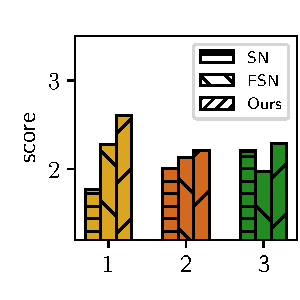
\includegraphics[width=1\textwidth]{chapters/vibvoice/figure/noise_number_0.pdf}
        %\vspace{-1.99em}
        \caption{PESQ.}
        \label{fig:vibvoice_noise_number_0}
        \end{subfigure}
        \hfill
    \begin{subfigure}{0.32\columnwidth}
        \centering
        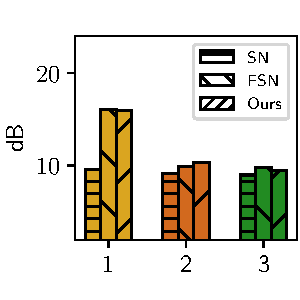
\includegraphics[width=1\textwidth]{chapters/vibvoice/figure/noise_number_1.pdf}
        %\vspace{-1.99em}
        \caption{SNR.}
        \label{fig:vibvoice_noise_number_1}
         \end{subfigure}
          \hfill
    \begin{subfigure}{0.32\columnwidth}
        \centering
        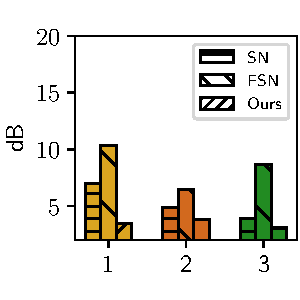
\includegraphics[width=1\textwidth]{chapters/vibvoice/figure/noise_number_2.pdf}
        %\vspace{-1.99em}
        \caption{LSD.}
        \label{fig:vibvoice_noise_number_2}
         \end{subfigure}
    %\vspace{-1em}
    \caption{Number of noise sources.}
    %\vspace{-1em}
    \label{fig:vibvoice_noise_number}
    % %\vspace{-1em}
\end{figure}




\begin{figure}
    \begin{subfigure}{0.3\columnwidth}
        \centering
        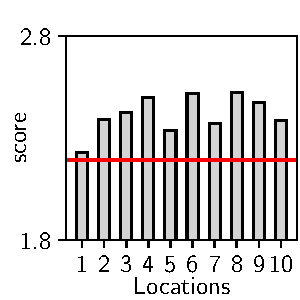
\includegraphics[width=1\textwidth]{chapters/vibvoice/figure/locations_0.pdf}
        %\vspace{-1em}
        \caption{PESQ.}
        \label{fig:vibvoice_location_0}
        \end{subfigure}
    \begin{subfigure}{0.3\columnwidth}
        \centering
        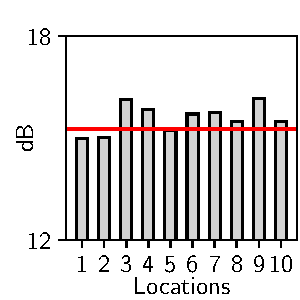
\includegraphics[width=1\textwidth]{chapters/vibvoice/figure/locations_1.pdf}
        %\vspace{-1em}
        \caption{SNR.}
        \label{fig:vibvoice_location_1}
         \end{subfigure}
    \begin{subfigure}{0.3\columnwidth}
        \centering
        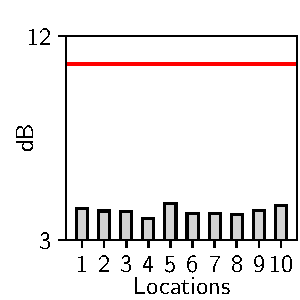
\includegraphics[width=1\textwidth]{chapters/vibvoice/figure/locations_2.pdf}
        %\vspace{-1em}
        \caption{LSD.}
        \label{fig:vibvoice_location_2}
         \end{subfigure}
    %\vspace{-1em}
    \caption{VibVoice on different head locations. Red line: the performance of the baseline, i.e., FullSubNet.}
    \label{fig:vibvoice_locations}
    %\vspace{-1em}
\end{figure}


\begin{figure}
    \begin{subfigure}{0.3\columnwidth}
        \centering
        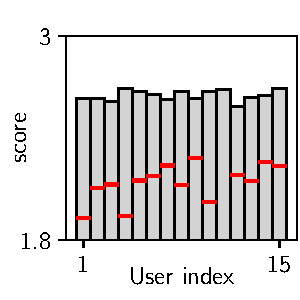
\includegraphics[width=1\textwidth]{chapters/vibvoice/figure/per_user_0.pdf}
        %\vspace{-1em}
        \caption{PESQ.}
        \label{fig:vibvoice_per_user_0}
        \end{subfigure}
    \begin{subfigure}{0.3\columnwidth}
        \centering
        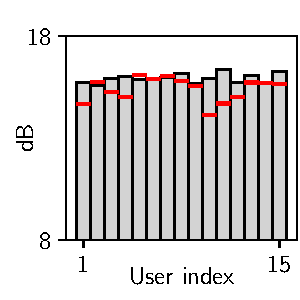
\includegraphics[width=1\textwidth]{chapters/vibvoice/figure/per_user_1.pdf}
        %\vspace{-1em}
        \caption{SNR.}
        \label{fig:vibvoice_per_user_1}
        \end{subfigure}
    \begin{subfigure}{0.3\columnwidth}
        \centering
        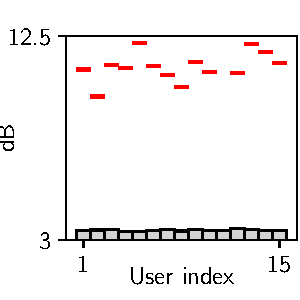
\includegraphics[width=1\textwidth]{chapters/vibvoice/figure/per_user_2.pdf}
        %\vspace{-1em}
        \caption{LSD.}
        \label{fig:vibvoice_per_user_2}
         \end{subfigure}
    %\vspace{-1em}
    \caption{VibVoice on different users. Red line: the performance of the baseline, i.e., FullSubNet.}
    \label{fig:vibvoice_per_user}
    %\vspace{-1em}
\end{figure}



\begin{figure}
% %\vspace{-1em}
    \begin{subfigure}{0.32\columnwidth}
        \centering
        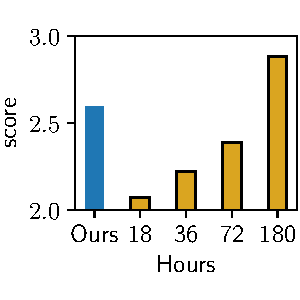
\includegraphics[width=1\textwidth]{chapters/vibvoice/figure/data_augmentation_0.pdf}
        %\vspace{-1.99em}
        \caption{PESQ.}
        \label{fig:vibvoice_data_augmentation_0}
        \end{subfigure}
    \begin{subfigure}{0.32\columnwidth}
        \centering
        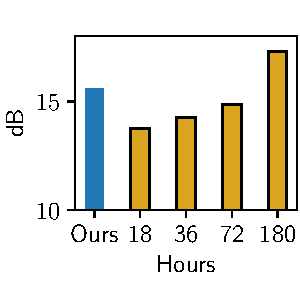
\includegraphics[width=1\textwidth]{chapters/vibvoice/figure/data_augmentation_1.pdf}
        %\vspace{-1.99em}
        \caption{SNR.}
        \label{fig:vibvoice_data_augmentation_1}
         \end{subfigure}
    \begin{subfigure}{0.32\columnwidth}
        \centering
        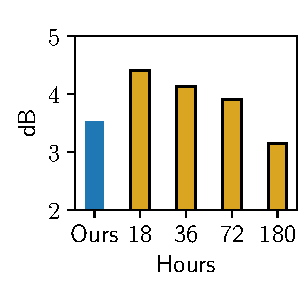
\includegraphics[width=1\textwidth]{chapters/vibvoice/figure/data_augmentation_2.pdf}
        %\vspace{-1.99em}
        \caption{LSD.}
        \label{fig:vibvoice_data_augmentation_2}
         \end{subfigure}
    %\vspace{-1em}
    \caption{Effectiveness of data augmentation. Blue bars: VibVoice using less than three-hour paired data with augmentation. Yellow bars: VibVoice using 18- to 180-hour paired data without augmentation.}
    \label{fig:vibvoice_data_augmentation}
\end{figure}

\begin{table}
\centering
\begin{tabular}{cccc}\toprule
& PESQ&SNR&LSD \\ \midrule
VibVoice              & 2.6 & 15.6 & 3.5  \\ 
w/o auxiliary decoder & 2.5 & 15.1 & 4.4 \\ 
w/o augmentation      & 1.9 & 14   & 5\\ 
w/o Gaussian approx   & 2.4 & 15.2 & 4.2 \\ 
Accelerometer sample rate: 1200 Hz & 2.47 & 14.4 & 4.2 \\ 
Accelerometer sample rate: 800 Hz & 2.45 & 14.3 & 4.5 \\ 
Accelerometer sample rate: 400 Hz & 2.4 & 14.2 & 4.4 \\ \bottomrule
\end{tabular}
\caption{\label{table3}Ablation study.}
\end{table}

\subsection{Ablation Study}
We conduct an ablation study to understand the performance of different design components in VibVoice. The performance of VibVoice without different components is listed in Table \ref{table3}.

\noindent\textbf{No auxiliary decoder}. First, we remove the self-supervise loss, meaning the audio may dominate the model. The results indicate that the variant slightly degrades by 0.1 in PESQ, 0.3 in SNR, and 0.8 in LSD, respectively.

\noindent\textbf{No data augmentation}.
Second, we remove the data augmentation based on Bone Conduction Function. The performance significantly degrades to 1.9 in PESQ, 14 in SNR, and 5 in LSD. According to the definition of ITU and mean opinion score (MOS), the audio quality is poor when the score drops from 2.5 to 1.9 \citep{Perceptu66:online}. This result aligns with our motivation that a small-scale self-collected dataset is insufficient to train a strong neural network.

\noindent\textbf{No Gaussian approximation}.
Third, the Bone Conduction Function is modeled by only the mean, while the variance is zero. The performance drops 0.2 in PESQ, 0.4 in SNR, and 0.5 for LSD, indicating that our Gaussian approximation is close to the nature of the Bone Conduction Function.

\noindent\textbf{Lower sample rate}.
The frequency response in Fig. \ref{fig:vibvoice_bcf} shows that the speech information from above 600 Hz is very limited. Hence, we evaluate the performance of VibVoice with a lower sample rate by downsampling the acceleration data to 1200 Hz, 800 Hz, and 400 Hz. The results show that VibVoice is robust to various sample rates, which consume less power in processing and communication. When the sample rate is 800 Hz, the output's PESQ only degrades $10\%$.

\subsection{On-Site Evaluation}
In the following, we conduct extensive experiments to validate the performance of VibVoice with ongoing noise in the wild. The volunteers are asked to read the same content as the experiments in Section. \ref{sec:vibvoice_overall_eval}. Apart from the environmental noises, we use a smartphone (i.e., Huawei P30) to play recorded speech and ask a volunteer to speak one meter away as the interference. The speech content of the competing speaker is irrelevant to the target speech. We collect 10 minutes of data with about 3dB SNR at each test location.
Unlike synthetic noisy speech, we can neither capture the ground truth of clean speech and evaluate the metrics like SNR and PESQ nor train the model. Instead, we use the result of Automatic Speech Recognition \citep{ravanelli2021speechbrain} to evaluate the quality of the speech. We use Word Error Rate ($\text{WER}=\frac{S+D+I}{N}$) as the evaluation metric, where S is the number of substitutions, D is the number of deletions, I is the number of insertions, and N is the number of words in the reference. The higher the value of WER, the lower the audio quality.
To better evaluate the performance of VibVoice, we further define the relative improvement of WER in percentage as $\frac{(WER_{o} -  WER_{v})}{WER_{o}}\times100 \%$, where $WER_{o}$ refers to the WER of the original audio, $WER_{v}$ refers to the WER of VibVoice.

\begin{figure}[t]
    \centering
    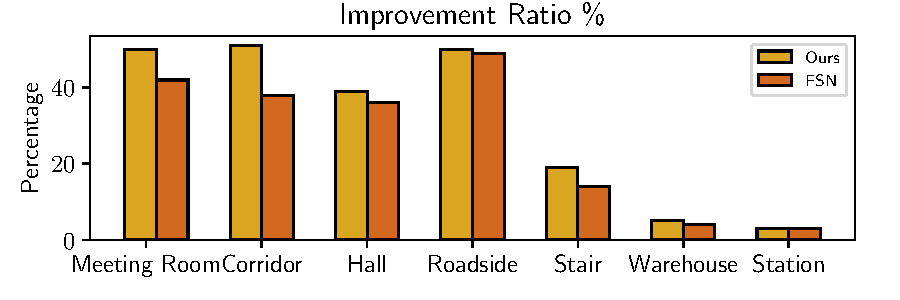
\includegraphics[width=\columnwidth]{chapters/vibvoice/figure/environments.pdf}
    %\vspace{-1em}
    \caption{Different environments.}
    %\vspace{-1em}
    \label{fig:vibvoice_environment}
\end{figure}

\subsubsection{\textbf{Environments}}
We evaluate VibVoice in diverse indoor and outdoor environments, including the meeting room, corridor, stairs, lumber room, and railway station. 
We note that the experiment conducted in the real world naturally contains diverse environmental noises (e.g., train, car, construction, wind) and competing speakers. The results in Fig. \ref{fig:vibvoice_environment} show that VibVoice effectively improves speech quality in most environments.
Most existing works have good performance in statistical noises like machinery noises, however, they perform badly when there are competing speakers in the same room, which is a common indoor scenario of voice communication.
 Although speech enhancement is challenging in small spaces like a meeting room and corridor due to the strong multi-path effect, VibVoice can still improve the speech quality and achieve an improvement ratio of over 50\%, and 48\%, respectively. VibVoice also achieves a 37$\%$ improvement for the hall, 29$\%$ for the outdoor square, and 19\% in the scene of the outdoor stair when there is intermittent construction noise. We note that in both the warehouse and station, the improvement of VibVoice is marginal. This is mainly because that AirPods already perform well in these scenarios. In comparison, VibVoice keeps outperforming FSN with much less latency. 

\subsubsection{\textbf{Earphones}}
We deploy VibVoice on three popular TWS earphones, i.e., Apple AirPods Pro, Huawei FreeBuds Pro, and Samsung GalaxyBuds Pro. During the experiment, we turn on all available acoustic signal processing algorithms provided by the manufacturers, including speech enhancement and noise suppression.
The results show that the WER with a competing speaker is $60\%$ for AirPods, $66\%$ for FreeBuds, and $160\%$ for GalaxyBuds, respectively. Due to the different designs of the earphones, we do not implement VibVoice on other earphones. Since VibVoice can effectively reduce the WER of AirPods Pro by $50\%$, we envision that VibVoice can be extended to other earphones.

\subsubsection{\textbf{User movements}}
We further evaluate the performance of VibVoice when the user is moving. We ask volunteers to move in the room with a speed of around $1\,\text{m/s}$.  
The result shows the improvement for a still volunteer is 58.3 $\%$, while the same moving volunteer is 57.1$\%$.
The standard deviation for the still and moving case is 29.9 $\%$ and 30.4$\%$, respectively. Although the improvement ratio slightly drops, VibVoice still preserves its performance under regular movements. 

\begin{table}
\centering
%\vspace{-1em}
\begin{tabular}{cccc}\toprule
& VibVoice & FSN & SN \\ \midrule
Desktop CPU    & 0.05 &0.27  & 0.5 \\ 
Desktop GPU    & 0.016&0.034 & 0.07\\ 
P30    & 0.16 &5     & 1.9 \\ 
Mate20 & 0.29 &4.6   & 1.7\\ 
Pixel7 & 0.31 &5.2   & 1.4\\ \bottomrule
\end{tabular}
\caption{\label{table4}Runtime analysis (second/instance).}
%\vspace{-1em}
\end{table}

\subsection{Runtime Evaluation}
\label{sec:vibvoice_runtime}
We test the execution latency of VibVoice and the two baselines (i.e., FSN \citep{hao2021fullsubnet} and SN \citep{tagliasacchi2020seanet}) on a desktop PC (i.e., i7-11700k CPU and RTX 3060 GPU) and three smartphones (i.e., Huawei P30, Huawei Mate20, and Google Pixel 7). We run the inference of 5 seconds clip 100 times and record the mean latency. 
The results in Table \ref{table4} show that VibVoice reduces up to $31\times$ and $12\times$ less latency on average than FSN and SN, respectively. On the other hand, the results show that VibVoice exhibits a greater advantage in runtime for low-end devices.
In conclusion, VibVoice can support real-time voice applications with a delay of fewer than 0.6 seconds (i.e., two times the inference latency) for processing 5 seconds audio clip. The real-time factor is only 0.12, significantly less than the minimal requirement, which means less energy consumption and space to process other tasks.

\section{User Study}
\label{sec:vibvoice_user-study}
We recruit 35 volunteers to study the real perceived experience of VibVoice.

%\vspace{0.5em}
\noindent\textbf{Questionnaire Design}.
We play a few recordings from the dataset described in Section 5.1 to volunteers. The length of each sentence is clipped or padded to 5 seconds.
The first part is to evaluate the intelligibility of reconstructed speech. The participants are asked to listen to the audio clips enhanced by VibVoice and write down the sentences. We use WER to evaluate the results.
In the second part of the study, participants listen to two audio clips with the same content and choose the audio with better quality in their perception. This study evaluates whether the reconstructed speech improves the user experience or not.
We conduct two kinds of comparisons five times. One type is to ask participants to choose between audio enhanced by VibVoice and the original noisy audio. The second kind is to ask participants to choose between audio enhanced by VibVoice and the baseline (i.e., FSN). We use the correct ratio $\frac{P}{P+N}$ to represent the improvement of VibVoice, in which $P$ and $N$ are the numbers of choosing VibVoice and negative vice versa.


\subsection{Study Result}
In the first part, VibVoice achieves an overall WER of $21.5\%$, which supports intelligibility of the reconstructed speech.
For perceived quality, $87\%$ of the participants choose VibVoice over the baseline, and $72\%$ choose VibVoice over the original noisy audio.
We also asked participants why they sometimes preferred the original audio over the baseline. The baseline can produce acoustic artifacts and suppress the target speaker. Some participants observed that repeated listening reduced the effect of artifacts and suppression, but the baseline speech still caused misunderstandings for first-time listeners. Overall, the user study shows that VibVoice improves perceived speech quality compared with both the original audio and the baseline.



\chapter{EgoLog: Ego-Centric Fine-Grained Daily Log with Ubiquitous Wearables}\label{ch:egolog}
This chapter presents EgoLog, a mobile sensing framework for daily logging with audio and motion sensors. It instantiates the \textit{fusion} dimension of user--environment coupling: EgoLog combines activity cues from HMWs with environmental scenario context, using companion mobile devices when needed. The thesis emphasizes HMWs because they are suitable for day-long use and provide stable egocentric audio--motion observations. EgoLog selectively separates user-generated and environmental signals, then fuses them with scenario context to achieve robust recognition in the wild.
The following sections describe the motivation, system design, and evaluation of EgoLog.

\section{Introduction}
\label{sec:egolog_intro}
\begin{figure}[ht]
  \centering
    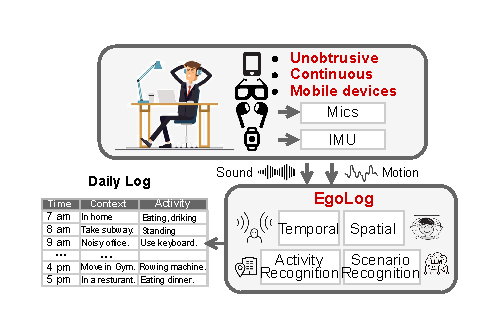
\includegraphics[width=1\linewidth]{chapters/egolog/figs/teaser.pdf}
    \caption{EgoLog uses microphones and an IMU on mobile and head-mounted devices for activity and scenario sensing.}
    \label{fig:egolog_teaser}
    \vspace{-1em}
\end{figure}

% HAR is important
Human activity recognition supports applications in physical and mental health monitoring, personalized healthcare, and daily routine analysis \citep{alam2014gesmart, gedam2021review}.
Smartphones and wearable devices can capture continuous sensor data during daily routines.
For example, motion data from an inertial measurement unit (IMU) can support human activity recognition because it reflects body movement. IMU-based systems have been developed for activities such as walking, standing, sitting, and lying~\citep{smartphonebased_recognition_of_human_activities_and_postural_transitions_341}.
Built-in microphones can also support acoustic scene recognition~\citep{martin2021low}, which provides contextual evidence for human activity.


% the limitation of previous work
However, existing HAR methods on mobile devices are limited to coarse-grained, scenario-constrained detection. For instance, step counting is a common application, but it fails to capture diverse activities such as cycling, swimming, or strength training. Although prior work has extended sensing to vital signs, gait analysis, and exercise recognition, these approaches often focus on isolated tasks rather than continuous daily monitoring.

% our problem/target
This chapter develops a mobile sensing system for ubiquitous devices, including earphones and smart glasses, to support continuous tracking of detailed egocentric human activities. The design models daily life from the user's perspective and moves beyond the recognition of short, isolated activities typically collected in laboratory settings. Fine-grained daily logging differs from conventional activity recognition in two ways:
\begin{enumerate}
    \item Daily life contains long-term activity structure, referred to here as ``scenarios.'' For instance, a user may spend an afternoon at the office while performing many related short-term activities.
    \item Daily life involves continuous interaction with the environment. Consequently, microphones capture sounds from the user, the environment, and other people. These environmental inputs can provide useful context, but they can also introduce noise.
\end{enumerate}


% device and modality
Several types of mobile devices are suitable for this task, including earphones, glasses, smartphones, and smartwatches. This thesis emphasizes head-mounted wearables because they are suitable for day-long use and provide stable egocentric observations, but the core audio--motion sensing design also applies to other mobile form factors. The available sensors can be roughly divided into two categories: visual and non-visual.
Visual sensors, such as cameras, can capture a first-person view rich with information. However, they are less practical for daily logging due to several limitations: 1) a limited field of view (FOV), 2) privacy concerns, and 3) high energy consumption for continuous sensing.
Instead, EgoLog uses non-visual sensors, namely motion and audio sensors. These sensors are widely available on smartphones, glasses, smartwatches, and earphones. As Fig. \ref{fig:egolog_teaser} shows, EgoLog continuously monitors a user's activities from an egocentric perspective and generates a daily log that includes both short-term activities and long-term scenarios.



% mobile devices have been a popular category of wearable devices that equip multiple sensors, such as microphones and IMUs. Being able to capture data from the user's ego view, mobile devices can be a desired platform for sensing detailed user-egocentric activities.
% First, earphone is the most popular wmobile devices with various applications including activity \citep{mollyn2022samosa}, speech \citep{he2023towards, dong2024rehearsse}, pose estimation \citep{duan2025argus}, eye tracking \citep{jiao2024medusa3d}, and vital signs \citep{chen2024exploring}.
% In 2025, there are more than 355 million mobile devices (e.g., earphones) sold, accounting for more than 60\% of wmobile devices worldwide \citep{Idc_2025}.
% Second, earphone is built with rich sensing capability, i.e., a microphone on each ear and an IMU. The sensors can capture stereo audio and motion that reflects egocentric information, such as user-induced speech and activities, and the location of environmental activities.
% Third, mobile devices are ideal for continuous sensing, the location of mobile devices is in the same place without the interference of the user's motion, and there is no blockage like a smartphone when it is placed in the pocket for most of the time.
% Besides, the average American young people use mobile devices more than 400 hours per year \citep{Ferjan_2022}, making it ideal for collecting continuous data.

This task introduces three challenges:
\begin{itemize}
    \item Existing mobile devices HAR models \citep{bhattacharya2022leveraging, gong2023mmg} lack the awareness of scenario information present in the real world. Specifically, user activities are driven by underlying reasons, and their distribution varies depending on the ``scenario.''  For instance, in an ``indoor cooking'' scenario, the ``jogging'' activity is less likely to happen.
    \item HAR models that depend on audio recordings are susceptible to interference due to the lack of spatial understanding. As a result, the audio data may lead to potential errors, which can be harmful for post-processing. For example, when detecting a ``clap'' activity based on sound, a nearby person's action could also trigger the model.
    \item Multi-modal fusion of audio and IMU is challenging and may not outperform a unimodal model \citep{huang2022modality}. Sensor heterogeneity weakens cross-modal alignment, as also observed in MMG-Ego4D \citep{gong2023mmg}. Effective fusion therefore requires models that identify when audio and motion are complementary.
\end{itemize}

To address these challenges, EgoLog uses the following design:
First, EgoLog recognizes long-term scenarios through temporal understanding, as detailed in Sec. \ref{sec:egolog_scenario}. This is achieved using a two-stage model: contrastive learning first projects audio and IMU features into a shared space to identify well-aligned segments as informative key frames; a sequence model then aggregates these key-frame features together with the original unimodal features for scenario recognition.

Second, EgoLog distinguishes user-generated activities from environmental sounds, including sounds produced by other people, through spatial understanding (Sec.~\ref{sec:egolog_localization}). The system formulates this as a sound localization task: near-field sounds are treated as user-centric events, while far-field sounds are treated as ambient background. A motion-aware localization model uses natural human movement and IMU readings to compensate for user motion and reduce spatial ambiguities such as near-far confusion.


Third, EgoLog introduces a multi-modal network for activity recognition that integrates audio, IMU, and scenario information (Sec.~\ref{sec:egolog_har}). Unlike short-term sensor data, the derived scenario captures longer-term behavioral patterns and provides high-level semantic cues for activity recognition.
The network uses dedicated unimodal backbones for feature extraction and a self-attention mechanism to dynamically fuse multimodal inputs, with scenario information encoded as a dense representation through a text encoder.

Finally, in Section \ref{sec:egolog_llm}, EgoLog introduces an edge-cloud framework assisted by a Large Language Model (LLM) for scenario recognition. The framework converts multi-modal data, including audio, IMU signals, sound localization outputs, and local scenario predictions, into contextual information for the LLM.
When the local model's prediction confidence is low, the edge device queries the cloud-based LLM. The refined scenario output is then used to update the local model over time.


We implemented and evaluated EgoLog on three large-scale public datasets, including Ego4D~\citep{grauman2022ego4d}, and a self-collected dataset covering multiple form factors, 10 participants, and 12 activities.
EgoLog improves activity recognition by 12\% and scenario recognition by 15\% over strong multi-modal baselines such as ImageBind~\citep{girdhar2023imagebind}, while keeping computation cost low.
The main contributions of this chapter are as follows:


\begin{itemize}
    \item
    EgoLog introduces an audio--IMU fusion method based on temporal and spatial understanding. It extracts scenario-level features through contrastive learning, aggregates them across short-term windows for scenario recognition, and integrates motion information with sound source localization for movement compensation.

    \item
    EgoLog develops an HAR method that takes both scenario context and raw sensor data as input. It uses scenario information to distinguish similar activities and uses sound-source estimates with audio--IMU correlation to separate user-generated sounds from background sounds.

    \item
    EgoLog introduces an LLM-assisted scenario recognition paradigm. Processed sensor data is fed into an LLM for high-level reasoning, and the LLM output is transferred back to the local device for on-device inference.

    \item
    EgoLog is evaluated on public datasets and a self-collected dataset, with an additional user study on the usefulness of generated daily summaries. The evaluation shows improvements of up to 15\% over the strongest baselines.
\end{itemize}

% \section{Related Work}

\label{sec:egolog_related}
\subsection{Motion Sensing for HAR}
IMU sensors in wearables and earables facilitate position tracking and user motion recognition, with their performance significantly impacted by sensor placement.
For example, LIMU-BERT \citep{xu2021limu} recognizes up to six activities with IMU recording of a smartphone.
Similarly, IMU on the wrist (e.g., smartwatch) can be used to recognize the basic activities \citep{chan2024capture}. 
Current motion sensing \citep{chan2024capture} only supports coarse-grained tasks, even with a large-scale dataset (>3000 hours), such as physical activity level (4 levels) or activities of daily life (10 activities).
Compared to smartphones and smartwatches, earables are a more reliable choice due to their relatively fixed position \citep{lyu2024earda, han2023headmon, han2023headsense, han2025headmon+}, as we illustrated before. Nonetheless, they share the same limitations in fine-grained motion sensing.

To enhance motion sensing, deploying multiple IMU sensors can enable precise full-body keypoint estimation with up to 17 IMUs. 
The pose of humans can be used to recognize fine-grained human activity, as demonstrated by MotionBERT ~\citep{zhu2023motionbert}. However, such an approach is impractical for everyday use. Instead, researchers propose leveraging commercial devices only, such as smartwatches, smartphones, and earables. For instance, combining multiple devices can enable fine-grained exercise activity recognition~\citep{stromback2020mm}. Similarly, IMUPoser achieves full-body pose estimation with just three IMUs~\citep{mollyn2023imuposer}. While using multiple devices improves performance, having all of them will have problems of high cost, user discomfort, setup complexity, and limited availability.

Another direction involves using pre-trained models to fuse IMU data with other modalities. Models like IMU2CLIP \citep{moon2023imu2clip} and ImageBind \citep{girdhar2023imagebind} link motion data to text or vision, enabling zero-shot recognition via retrieval. However, their performance on fine-grained tasks remains limited. Recently, Large Language Models (LLMs) have shown promise in reasoning over motion data \citep{ji2024hargpt, leng2024imugpt, xu2024autolife, ouyang2024llmsense}, often by converting sensor readings into text tokens for the LLM to process \citep{xu2024penetrative}.


% To further improve motion sensing, integrating advanced pretrained models that incorporate multiple modalities, such as text, offers a promising approach. Models like IMU2CLIP~\citepp{moon2023imu2clip} and ImageBind~\citep{girdhar2023imagebind} connect motion data to other modalities, enabling zero-shot activity recognition through retrieval. 
% However, their performance remains limited. For instance, IMU2CLIP \citepp{moon2023imu2clip} is restricted to four-class activity recognition, while ImageBind \citepp{girdhar2023imagebind} achieves only 25\% accuracy on fine-grained activity recognition.

% Recently, LLMs have demonstrated exceptional reasoning abilities when working on not only vision and text \citep{yang2024viassist, liu2023improved}, but also other modalities like motion \citep{ji2024hargpt, leng2024imugpt, xu2024autolife, ouyang2024llmsense}. For example, Penetrative AI \citep{xu2024penetrative} has shown that LLMs can also interpret sensor data such as accelerometers. 
% All of the above works convert the raw data into strings that can be easily accepted by LLM.

In summary, prior work on motion sensing either employs multiple IMU sensors or remains confined to coarse-grained activity recognition. Since IMU sensing inherently
lacks contextual or environmental information, which limits their ability to perform fine-grained HAR \citep{tong2020accelerometers}. Further advancements should focus on integrating additional modalities or external knowledge.

\subsection{Acoustic Sensing for HAR}
In addition to IMU sensors, acoustic sensors (microphones and speakers) are also commonly integrated into wearables and mobile devices. The use of a speaker allows acoustic sensing to be categorized into two approaches: active sensing (utilizing both the speaker and the microphone) and passive sensing (using only the microphone).

As the main research area of audio, there are multiple applications of passive audio sensing, including speech recognition and audio classification \citep{schmid2023efficient}. However, audio is related but does not directly reflect human activity. Instead, it relies on the sound caused by activity, which can be easily misled by a loudspeaker. As a result, audio-based HAR is often treated as a specialized form of audio classification \citep{cristina2024audio}.
In contrast, multi-channel passive sensing enhances spatial awareness by estimating the direction of arrival (DoA) of sounds using microphone arrays \citep{schmidt1986multiple, adavanne2018sound} or binaural earables \citep{yang2022deepear, krause2021joint}. While DoA provides useful context, it cannot confirm whether the source is human or differentiate the loudspeaker. To detect human presence, some approaches integrate feedforward microphones to capture vocal activity via head-related sounds \citep{zhang2024earsavas}, or use an IMU to capture the bone-conduction sound \citep{he2023towards}. However, they can only cover the vocal activity.

Different from passive sensing, active sensing analyzes transmitted acoustic waves and their reflections, enabling non-contact sensing.
For the context of human activity, we are more interested in 
sensing not only the facial movements \citep{dong2024rehearsse} with outward-facing speaker, such as upper body pose detection \citep{mahmud2023posesonic}, and gesture recognition \citep{yang2024maf}. However, the speakers are usually oriented inward or designed to be effective only in the near field to maintain user privacy, which hugely limits the performance in coarse-grained recognition. 

In summary, acoustic sensors in wearables enable rich information capture through either passive or active sensing. However, audio-based HAR is still limited, as passive sensing struggles to confirm human presence, and active sensing is constrained by practical considerations, necessitating multi-modal integration for improved performance.

\subsection{Multi-modal Sensing for HAR}
Multi-modal learning of audio and IMU data addresses limitations in motion sensing or acoustic sensing by leveraging the complementary strengths of both modalities. For instance, VibVoice \citep{he2023towards} uses bone-conduction vibration and audio in earables to distinguish a user’s voice from others. Similarly, \citep{min2018exploring} employs IMU for motion detection and a microphone for conversation detection, processed independently. Other wearables, such as wrist-mounted or head-mounted devices, also utilize multi-modal approaches; SAMoSA \citep{mollyn2022samosa, bhattacharya2022leveraging} integrates audio and IMU on smartwatches to recognize up to 26 activities. However, multi-modal learning is not universally superior, as its effectiveness depends on factors like data quality, modality correlation, and model design. 
For example, the fusion of audio and IMU on a diverse dataset like Ego4D \citep{grauman2022ego4d} can be challenging.
As demonstrated by MMG-Ego4D \citep{gong2023mmg}, where a multi-modal model for smart glasses underperformed compared to single-modal models in recognizing nearly 200 actions, highlighting that multi-modal approaches do not always guarantee improved performance \citep{huang2022modality}.

Beyond integrating audio and IMU sensors, incorporating additional knowledge sources can enhance motion sensing. For example, SAMoSA \citep{mollyn2022samosa} uses automatic context detection to trigger context-specific classifiers, though limited to predefined classes. Furthermore, the advanced LLMs facilitate multi-modal processing, either at the prompt level, incorporating IMU, GPS, Wi-Fi, or Bluetooth data \citep{yang2025contextagent, xu2024autolife,yang2024drhouse}, or at the token level, combining audio and IMU \citep{han2023onellm, girdhar2023imagebind}. While promising, those works lack explicit multi-modal fusion, especially for the heterogeneous multi-modal data from mobile devices.

In summary, the fusion of audio and IMU can be challenging since the correlation between them can be weak. While incorporating external knowledge or using powerful models like LLMs for fusion can enhance recognition, current methods still lack effective techniques for deeply integrating the heterogeneous data.
\section{Motivation Study}
\label{sec:egolog_measurement}
As discussed in Sec. \ref{sec:egolog_intro}, we mainly have three challenges towards a multi-modal HAR on mobile devices: 1) lack of scenario awareness, 2) being sensitive to ambient noise, and 3) fusion collapse. To explore these challenges and evaluate the potential for overcoming them, we conduct a series of experiments to analyze and demonstrate promising directions.

\begin{figure}
    \centering
    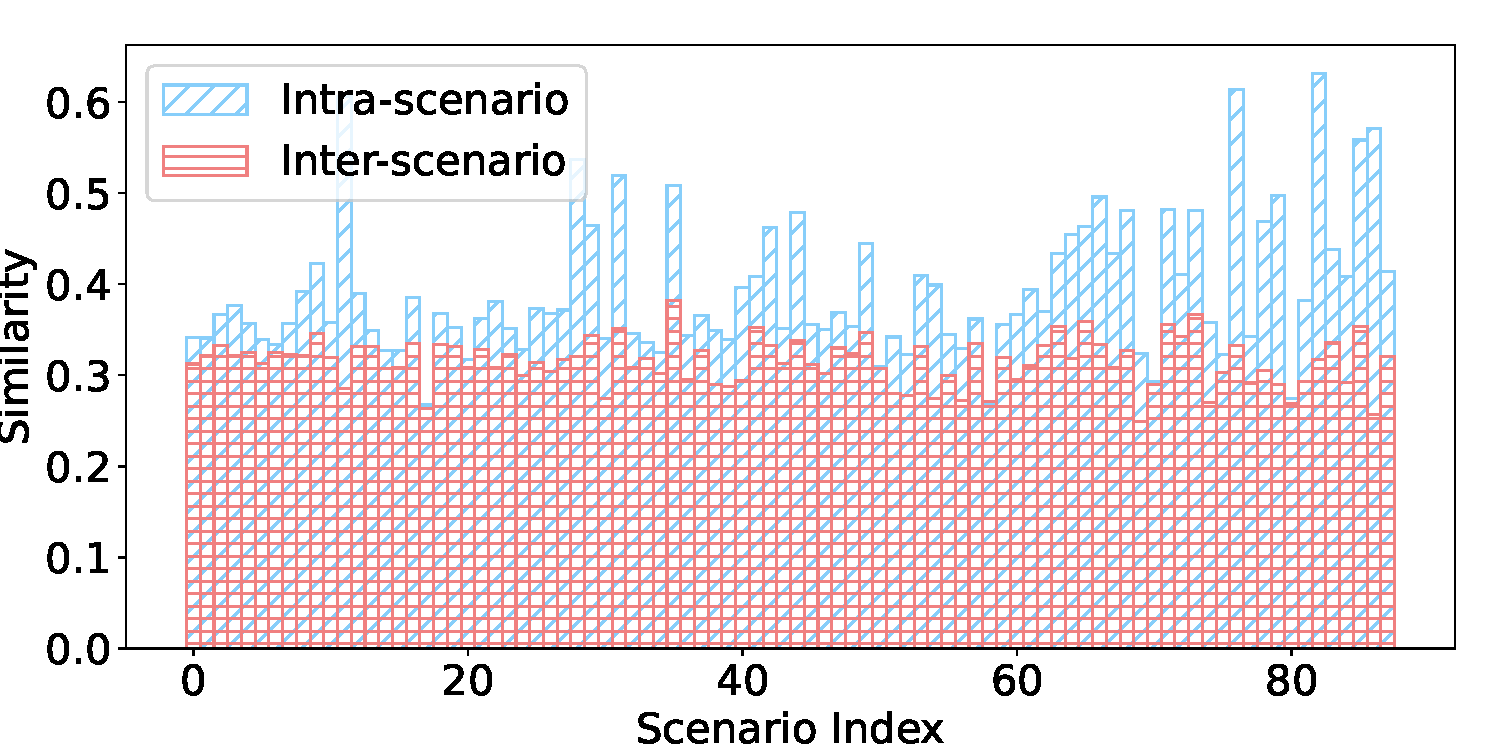
\includegraphics[width=0.8\linewidth]{chapters/egolog/figs/scenario_similarity.pdf}
    \vspace{-1em}
    \caption{Motivation for scenario understanding: 
    The similarity of embeddings for intra- and inter-scenario activities.}
    \label{fig:egolog_scenario_similarity}
    \vspace{-1em}
\end{figure}

\subsection{Scenario}
\label{subsec:scenario}
Scenario information refers to long-time activities (e.g., playing with a pet or working at home) that reflect the user's real-world behavior. Capturing such scenarios in datasets is challenging, as it requires volunteers to perform activities naturally, mimicking real-life conditions. Generally, scenario is the ensemble of multiple related and continuous activities with a realistic distribution, reflecting meaningful interactions with the environment.

To investigate the impact of scenario information on HAR, we use the Ego4D dataset~\citep{grauman2022ego4d}, which captures real-world activities through smart glasses equipped with IMU and audio sensors. The dataset provides annotations at both the window level (every 10 seconds) and the video level, represented as plain text. We treat window-level annotations as activity labels and video-level annotations as scenario labels that describe the broader setting of prolonged activities. To examine scenario properties, we use Sentence-BERT~\citep{reimers2019sentence} to generate text embeddings for activities across 91 scenarios. We then compute activity similarity both within scenarios (intra-scenario) and between scenarios (inter-scenario). Intra-scenario similarity measures the similarity of activities within the same scenario, while inter-scenario similarity compares an activity from one scenario to a randomly selected activity from a different scenario.

The results are shown in Fig.~\ref{fig:egolog_scenario_similarity}, revealing that the similarity within a scenario (intra-scenario similarity) is over 20\% higher than the similarity between different scenarios (inter-scenario similarity). This suggests that each scenario has a distinct distribution of activities. Specifically, a scenario effectively represents the user's daily log since it encompasses a longer time frame.
Additionally, we notice that the inter-scenario similarity is generally above 0.3, indicating that many basic activities (such as sitting and walking) are common across all scenarios. Therefore, it is crucial to eliminate the influence of these basic activities in scenario recognition, as they are present in every scenario.


In summary, the in-the-wild dataset shows that scenarios have distinct activity distributions, which can support scenario recognition through scenario-specific activities.


\subsection{Sound Location }
\label{subsec:embodied}
\begin{figure}
    \centering
    \begin{minipage}{0.48\linewidth}
        \centering
       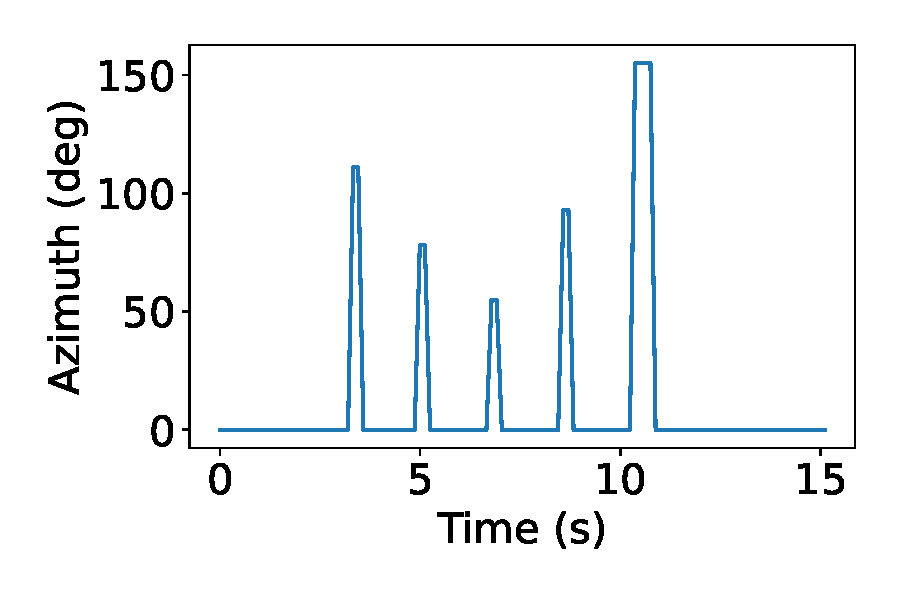
\includegraphics[width=\linewidth]{chapters/egolog/figs/baseline_result.pdf}
        \caption{Sound localization \citep{schmidt1986multiple} under motion}
        \label{fig:egolog_loc_move}
    \end{minipage}
    \hfill
    \begin{minipage}{0.48\linewidth}
        \centering
        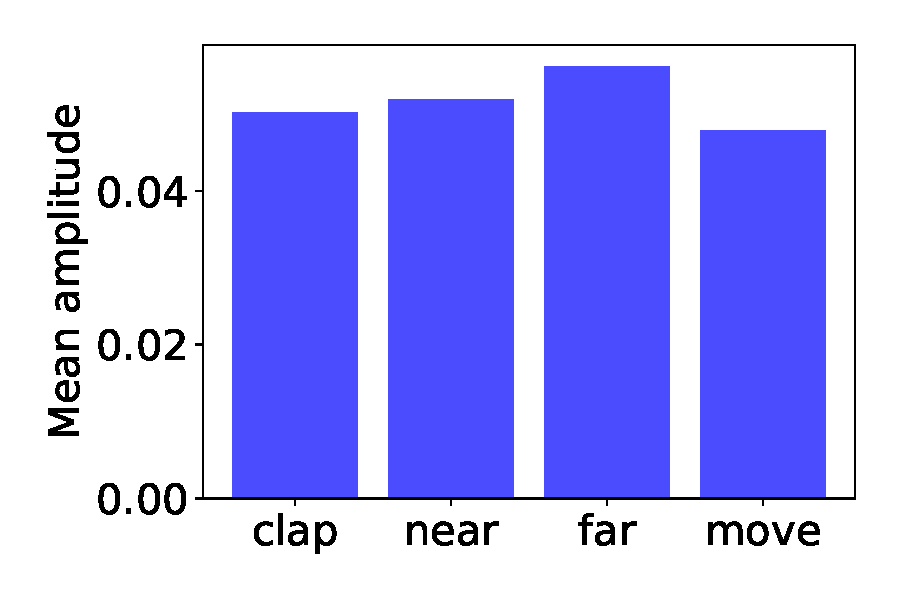
\includegraphics[width=\linewidth]{chapters/egolog/figs/amplitude.pdf}
        \caption{Sound volume may not related to distance.}
        \label{fig:egolog_amplitude}
    \end{minipage}    
    \vspace{-1em}
\end{figure}

\begin{figure}
    \centering
    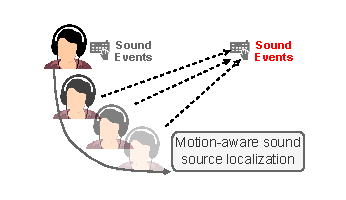
\includegraphics[width=0.75\linewidth]{chapters/egolog/figs/spatial_motivation.pdf}
    \vspace{-1em}
    \caption{Motivation for spatial understanding: estimate the distance of a sound event by motion.}
    \vspace{-1em}
    \label{fig:egolog_motivation_localization}
\end{figure}

In practice, recorded audio often includes far-field sound sources that are unrelated to the user’s activities, underscoring the importance of sound localization for effective HAR. Wearables that are consistently worn on the user’s head provide a stable and reliable position for capturing detailed ambient sound information. Additionally, modern wearables feature multi-channel recording capabilities, enhancing their spatial sensing potential.
In the following, we divide sound localization into direction and distance estimation, which we discuss as follows.

The estimation of sound direction is one of the mature, basic, but still challenging applications of a microphone array. The accuracy highly depends on the number of microphones, which is unfortunately not sufficient for most commercial devices. Considering the most common setting of stereo recording, there are mainly two problems: the deviation of direction (especially for front-back confusion) and estimation of sound distance, as illustrated in Fig. \ref{fig:egolog_motivation_localization}.
We envision that the above challenges may be solved by motion compensation. Specifically, we can aggregate the consecutive sound localization results along with the movement of the user (microphone) to refine the results or even get the distance.

To illustrate these challenges, we positioned a sound source in front of the user and used a binaural microphone with the algorithm from~\citep{schmidt1986multiple} to estimate direction of arrival, as shown in Fig.~\ref{fig:egolog_loc_move}. The user was instructed to move the body slightly and naturally. The estimate fluctuated around the true value of 90 degrees. To test whether sound volume is sufficient for differentiating near and far sources, we conducted an experiment with the sound source at different distances from the microphone. As shown in Fig.~\ref{fig:egolog_amplitude}, volume differences were not reliable across distances. The final bar in Fig.~\ref{fig:egolog_amplitude} also shows that user movement slightly affects amplitude. Multiple sound sources can further complicate volume-based distance estimation.

\subsection{Multi-modal Fusion }
\label{subsec:measure-fuse}

\begin{figure}
    \centering
     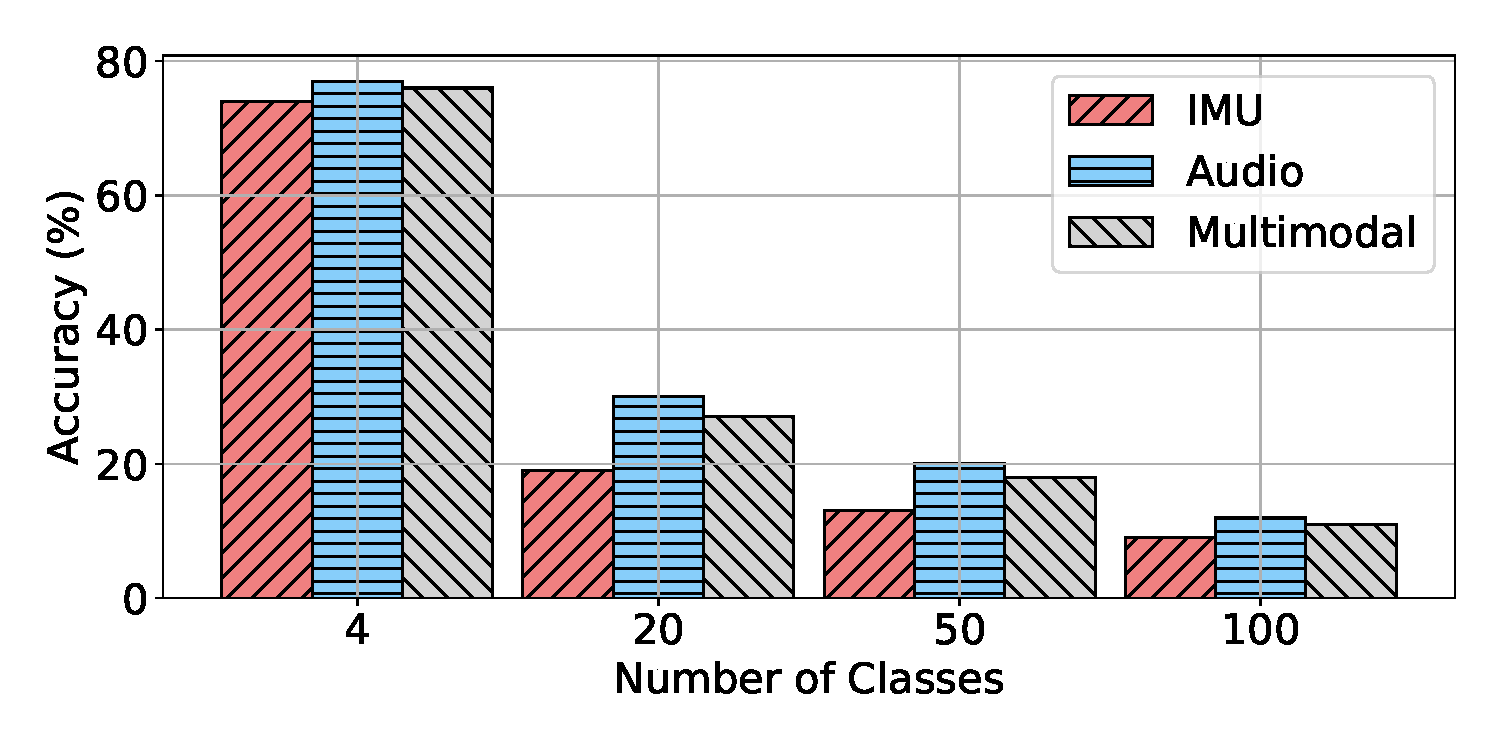
\includegraphics[width=.75\linewidth]{chapters/egolog/figs/num_class.pdf}
     \vspace{-1em}
      \caption{The performance of an existing activity recognition with different class numbers and modalities.}
    \label{fig:egolog_num_class}
    \vspace{-1em}
\end{figure}

To investigate scalability bottlenecks in activity recognition using wearables, we trained unimodal supervised models with audio and IMU data on the Ego4D episodic memory subset (200 activity classes). We used EfficientAT~\citep{schmid2023efficient} for audio and LIMU-BERT~\citep{xu2021limu} for IMU as feature extraction backbones, comparing them to a multi-modal model via late fusion. Activities were clustered into varying class numbers using Sentence BERT~\citep{reimers2019sentence} embeddings and K-Means~\citep{macqueen1967some}, following MMG-Ego4D~\citep{gong2023mmg}. Results (Fig.~\ref{fig:egolog_num_class}) show a significant performance drop as class numbers increase, indicating challenges in recognizing diverse activities with audio or IMU alone. Multimodal fusion often underperforms unimodal models, suggesting ineffective extraction of complementary features at larger scales.

\begin{figure}
    \centering
    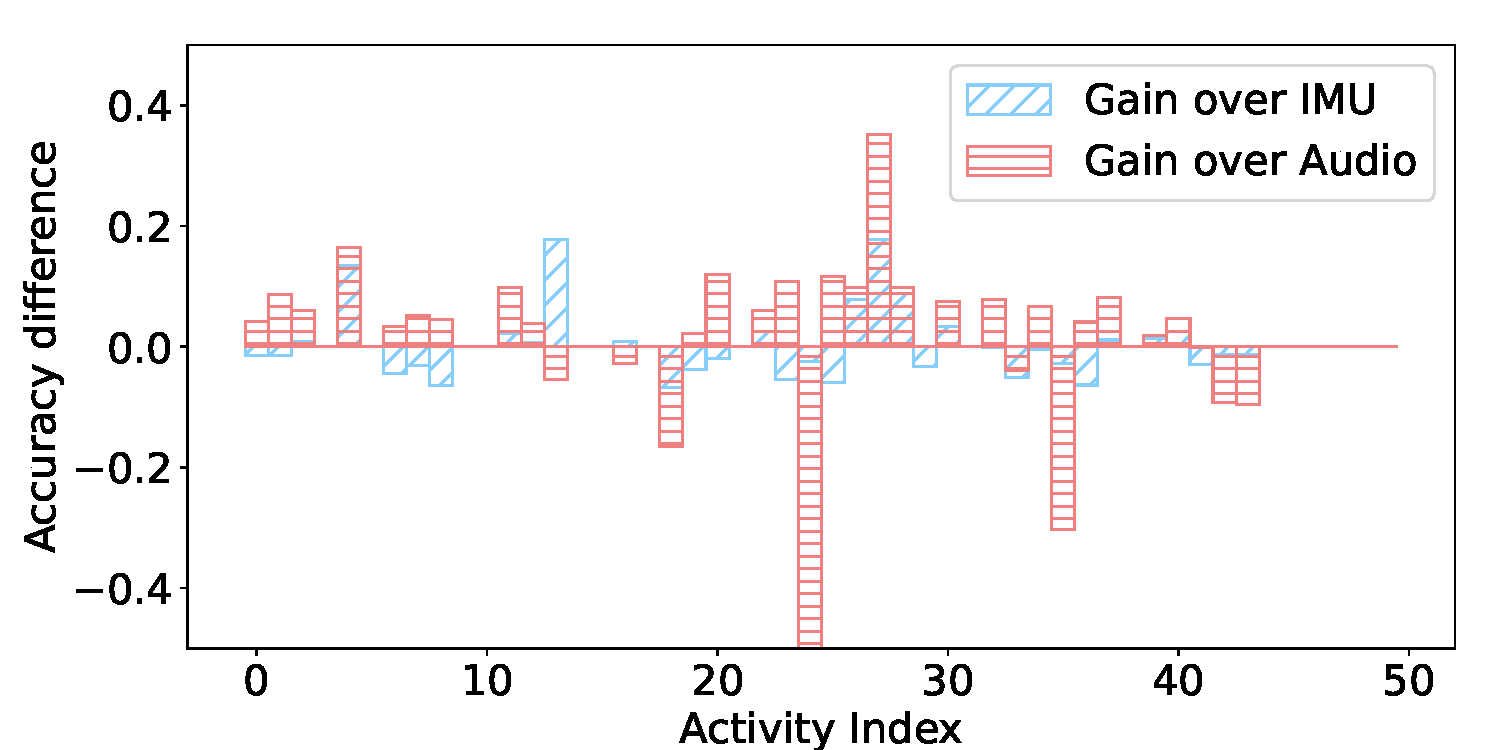
\includegraphics[width=.75\linewidth]{chapters/egolog/figs/activity_diff.pdf}
    \vspace{-1em}
    \caption{Performance gain from multi-modal fusion.}
    \label{fig:egolog_acc_gap}
    \vspace{-1em}
\end{figure}

Previous work~\citep{mollyn2022samosa} demonstrates that multi-modal learning can outperform the unimodal model due to the complementary nature of each other.
However, this finding does not apply to all cases. Another study~\citep{gong2023mmg} finds that multimodal learning with audio and IMU on Ego4D can perform worse than single-modality solutions. To investigate this result, we compared the accuracy of multimodal and unimodal models for each class, as shown in Fig.~\ref{fig:egolog_acc_gap}. The benefits of multimodal fusion fluctuate across both modalities, indicating that supervised multimodal learning cannot automatically select the appropriate modality for each activity.


To investigate whether LLMs can alleviate this problem, we evaluate ImageBind-LLM~\citep{han2023imagebind}, which converts both modalities into features and prepends them to text embeddings. We instruct the model with the prompt: ``<sensor> According to the audio and IMU reading on the earphone of the user, what is the activity of the user?'', where <sensor> denotes the inserted sensor features. Since LLM outputs can be random, we also constrain the prompt to one of the candidate activities. To reduce complexity, we select the top 30 activities from the Ego4D episodic memory subset. ImageBind-LLM achieves BERT-score precision, recall, and F1 score of 0.04, 0.07, and 0.05, respectively. Because this performance is low, we inspect the outputs and find that the LLM may not fully understand the multimodal fusion task.
We further test whether fine-tuning can address this problem by training an adapter~\citep{zhang2023llamaadapter} for ImageBind-LLM. The adapted LLM achieves BERT-score precision, recall, and F1 score of 0.47, 0.46, and 0.47, respectively. Although fine-tuning improves performance, the result remains below the level needed for practical use.

\section{System Design}
\begin{figure*}
    \centering
    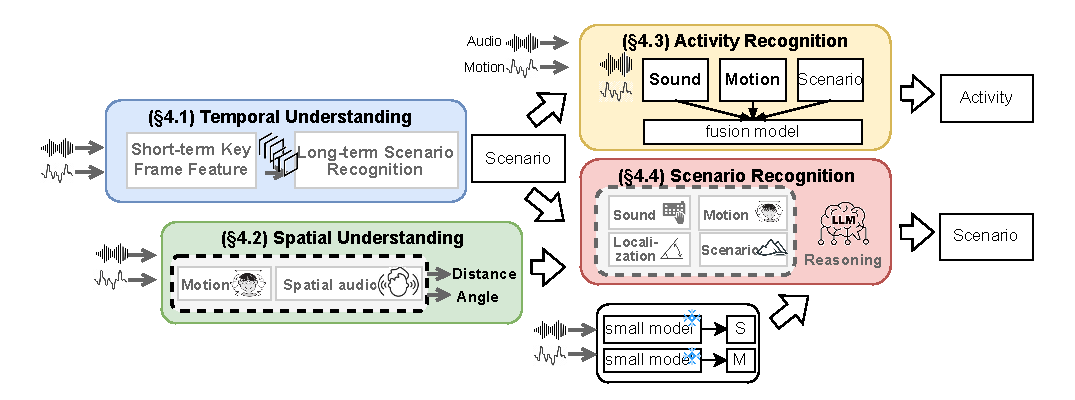
\includegraphics[width=0.8\linewidth]{chapters/egolog/figs/overview.pdf}
    \vspace{-1em}
      \caption{The system overview of EgoLog: the temporal and spatial understanding are two modules for multi-modal fusion, providing important input to the later modules to recognize activity and scenario}
      \vspace{-1em}
    \label{fig:egolog_system}
\end{figure*}

Figure~\ref{fig:egolog_system} provides an overview of EgoLog, a mobile system designed to capture egocentric daily logs over both long-term and short-term periods. 
Specifically, Section~\ref{sec:egolog_scenario} and Section~\ref{sec:egolog_localization} detail the fusion of audio and IMU data to achieve a deeper understanding of scenario (i.e., long-term descriptions) and spatial information (i.e., the relative location of sound sources). These insights serve as foundational clues for subsequent processing. 
In Section~\ref{sec:egolog_har}, we integrate the scenario information into the multi-modal activity recognition process, effectively mitigating modality collapse. Finally, Section~\ref{sec:egolog_llm} describes the use of an LLM as an expert to refine the scenario recognition from the previous stage; the resulting knowledge is subsequently transferred back to the local device.


\subsection{Temporal Understanding}
\label{sec:egolog_scenario}

\begin{figure}
  \centering
    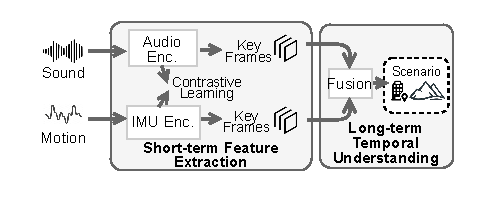
\includegraphics[width=1\linewidth]{chapters/egolog/figs/scenario.pdf}
    \vspace{-1em}
    \caption{Temporal understanding: we use contrastive learning to extract the cross-modal feature, which is important for the temporal-level fusion that recognize the scenario.}
    \vspace{-1em}
    \label{fig:egolog_scenario-recog}
\end{figure}

The measurement study indicates that recognizing many activities using IMU or audio data with an end-to-end model is difficult.
EgoLog therefore uses scenario recognition to provide prior information for activity recognition (Section~\ref{sec:egolog_har}). Scenario recognition also provides a useful high-level summary for daily logs.
As previously discussed, a scenario can be considered as a long-duration activity composed of multiple correlated sub-activities. To achieve accurate recognition, it is essential to develop an improved method for temporal analysis.
The pipeline is illustrated in Fig.~\ref{fig:egolog_scenario-recog}.


\subsubsection{Problem analysis}
Audio and IMU data have different properties and advantages. Their pretrained encoders are therefore optimized for different objectives. Simply merging their outputs may not produce the best results, as shown in Sec.~\ref{sec:egolog_measurement}; effective fusion must account for the heterogeneity of the two modalities.

We aim to tackle scenario recognition, which refers to identifying high-level human activities over an extended period (over 30 seconds). As detailed in Sec.~\ref{sec:egolog_measurement}, current pre-trained encoders already hold some scenario-level information, although they still fall short of ideal performance. A straightforward approach involves training a classification model using a dataset annotated with scenarios in an end-to-end fashion. Nonetheless, we have identified two persisting challenges: (1) the end-to-end model may struggle to generalize across different input lengths. (2) The performance might be inferior if scenarios are not included in the training data. Therefore, we propose training a new encoder for two modalities to obtain scenario-level features from brief time windows, which will then be applied in a secondary scenario recognition phase.

Given audio data and IMU data, the corresponding annotations for activity and scenario are assigned. Ideally, we could estimate activities individually and recognize scenarios accordingly. However, many activities may not relate to the audio or IMU data, such as silent motions that exceed the audio's capability.
Instead, we propose using two encoders: one for audio and one for IMU data. Their outputs would project the same feature space, representing features of the same scenario. Like activities, the two modalities may not always directly correlate with the scenario, so the mapping can fail sometimes. To address this, we can estimate the scenario by combining multiple windows of data, compensating for the sparsity of features.

\subsubsection{Contrastive learning}
Based on the preceding analysis, employing contrastive learning is optimal for capturing scenario-level features. Contrastive learning focuses on acquiring low-dimensional representations ($SE_i$) by differentiating between similar and dissimilar data samples. The method aims to group similar samples closely in the representation space while distancing dissimilar ones using the Euclidean distance. The efficacy of contrastive learning has been demonstrated in earlier research~\citep{han2023onellm, girdhar2023imagebind}. 
Within our framework, similarity and dissimilarity can be defined in two ways. Firstly, any data point aside from itself is deemed dissimilar. Secondly, data points within the same scenario are viewed as similar, whereas others are regarded as dissimilar. We expect that the first approach will yield more robust features, since it does not rely on explicit scenario annotations, and this will be assessed during the evaluation.

Regarding the network design, we employ two distinct deep neural networks to derive embeddings: LIMU-BERT~\citep{xu2021limu} for the IMU data and EfficientAT~\citep{lyu2024earda} for the audio input. Each sample spans a two-second window. The training of both encoders is based on the cross-entropy loss function, structured as follows:
\[
logits = (Audio_e \cdot IMU_e^T) \cdot \exp(\tau),
\]
where $Audio_e$ and $IMU_e$ refer to the features from two encoders, and $\tau$ refers to the learned temperature parameter \citep{chen2020simple}. Then, we get the loss using cross-entropy loss as follows:
\[
L = cross\_entropy\_loss(logits, label, axis=0).
\]

\subsubsection{Scenario recognition}
Assuming we extract the features from $Audio_e$ and $IMU_e$ by contrastive learning, they may not immediately convey the scenario as previously noted. We observe that a robust example in which both modalities relate to the scenario will exhibit a strong similarity between $Audio_e$ and $IMU_e$. This high similarity indicates that both modalities are effectively mapped into the same feature space, highlighting their importance as key features.
Conversely, low similarity suggests that the two modalities have not been successfully integrated into a unified representation of the scenario. Ideally, we would only keep frames with high similarity. However, the dynamics of execution can be problematic, introducing instability. Furthermore, it is difficult to set a definitive threshold to classify all frames below it as "useless."
Given the inherently weak correlation between audio and IMU, examples with high similarity may be rare. The model therefore needs to use as much information as possible from the available data.
To address this problem, we propose extending the key features along the temporal dimension. We integrate a sequence model—either an LSTM or a transformer—to compile features over time (as shown in the right section of Fig.~\ref{fig:egolog_scenario-recog}).
This two-stage architecture enables the model to capture both short-term and long-term dependencies within the features, thereby improving the accurate recognition of extended scenarios. Finally, a linear layer followed by a sigmoid activation function is used to predict the probability for each scenario.

\begin{figure}
  \centering
    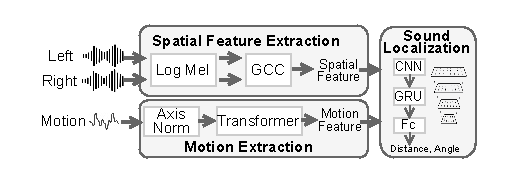
\includegraphics[width=1\linewidth]{chapters/egolog/figs/localization.pdf}
    \vspace{-1em}
    \caption{Spatial understanding: we differentiate sound by location by the combination of spatial audio and motion, leveraging the natural but random movement of the user.}
    \label{fig:egolog_seldnet}
    \vspace{-1em}
\end{figure}


\subsection{Spatial Understanding}
\label{sec:egolog_localization}
Existing activity recognition methods by audio are often misled by environmental events.
As illustrated in Sec. \ref{sec:egolog_measurement}, it is not enough to use sound volume to differentiate the near-field and far-field sound. Here, we are interested in the near-field sound because of the close correlation between it and the user's interaction with the environment. 

\subsubsection{Sound localization}
The location of sound can be estimated by a multi-channel microphone array. 
Specifically, the time of arrival of the sound source for one microphone is: \(t_i = \frac{\sqrt{(x_s - x_i)^2 + (y_s - y_i)^2}}{c}\), where the location of microphones $\mathbf{p}_i = (x_i, y_i)$, $i = 1, \ldots, N$, and a sound source at $\mathbf{s} = (x_s, y_s)$.
Since the start time of the sound source is unknown, the system can only obtain the time difference of arrival (TDoA) between two microphones, such as $i$ and $j$. With only two microphones on binaural earables, this yields a single equation, which is insufficient to resolve front--back confusion reliably.

Building on the work of SELDNet \citep{adavanne2018sound} and DeepEar \citep{yang2022deepear}, we propose a neural network-based binaural localization. Overall, our model performs an 8-class classification, distinguishing between four directions (front, left, right, back) and two distance categories (near and far). The binaural audio input, is converted to two log-Mel spectrograms and generalized cross-correlation coefficients of spectrograms, combined along the channel dimension to form spatial features with shape \( B \times 3 \times T \times 64 \), where \( B \) is the batch size and \( T \) is the number of frames. We process the audio feature with three convolutional layers, transforming it to (B, 128, T/5, 64). Then it is followed by a GRU layer, multi-head attention (resulting in B, 128, T/5, 64), and a linear layer that outputs (B, T/5, C).


\subsubsection{Movement compensation}

As illustrated in the motivation study, user movement can improve spatial understanding. Similar ideas have been used in prior work~\citep{zhu2021localizing, seo2022ross}, but these approaches require either explicit user gestures or a fully controllable robot. EgoLog instead uses natural, unintentional body movements that occur in daily life.

To realize this, we introduce an end-to-end method where IMU data—structured as (B, 6, T) and comprising both accelerometer and gyroscope measurements—is processed through two transformer layers. This module outputs a representation of shape (B, 384, T), which is then passed through a linear layer to produce an output of size (B, T/5, C). The resulting features are subsequently concatenated with the output from the GRU module.
The overall model performs an 8-class classification (C=8), distinguishing between four spatial directions (front, left, right, back) and two distance categories (near and far).

EgoLog cannot assume that only one sound source exists. Multiple sound sources may overlap, and both sound localization and audio recognition can be multi-label. This creates an association problem, which is addressed in a later section.

\subsection{Scenario-aware Activity Recognition}
\label{sec:egolog_har}

\begin{figure}
    \centering
    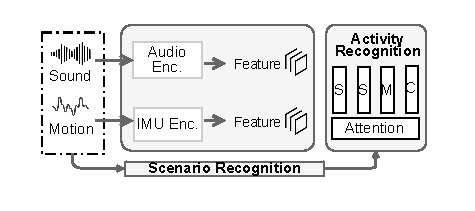
\includegraphics[width=1\linewidth]{chapters/egolog/figs/activity_recognition.pdf}
    \vspace{-1em}
    \caption{Multi-modal activity recognition: We extract features from each individual modality (uni-modal features), combine them with the scenario information derived from temporal understanding, and merge them at the token level for final activity recognition.}
    \vspace{-1em}
    \label{fig:egolog_activity_recognition}
\end{figure}

The methods outlined in Sec. \ref{sec:egolog_scenario} and \ref{sec:egolog_localization} offer a promising path for audio-IMU fusion. Next, we propose to integrate them into HAR.

Our proposed multi-modal network consists of two main components: unimodal backbones and a fusion module. The unimodal backbones include separate feature extractors that gather features from each input modality. The fusion module is designed to combine and aggregate these features from the unimodal backbones, resulting in a fused output that denotes the activity of the user. Although the design described above shows promise, it shares similar input and output characteristics with those presented in Section \ref{sec:egolog_measurement}, which has already been validated. As a result, it may not perform well in human activity recognition due to a lack of multi-modal correlation.

There are two common approaches for fusing modalities: using a multi-layer perceptron to process concatenated representations, or using a Transformer-based fusion module that processes a sequence of tokens from different modalities~\citep{gabeur2020multi}. EgoLog uses the Transformer-based design because attention can scale to a variable number of input tokens.
This flexibility is particularly important, as our multi-modal model needs to handle data with a varying number of modalities (more than only audio and IMU) for the task. Specifically, suppose the scenario information is a feature with the same dimension as other modalities, the transformer module can easily integrate it.
The final output of the fusion module is calculated by averaging the output tokens, rather than relying on the CLS token. The formulation of the token for one modality $Z_m$ is below:
\[
Z_m = (Encoder_m(S_m), e_m), \quad Z=f(Z_1, Z2, Z_3...)
\], where \( m \) represents each modality, which includes audio, IMU, and text. The term \( e_m \) denotes the learnable embedding specific to each modality. The transformer fusion module will combine multiple \( Z_m \) tokens and produce a unified \( Z \) feature with consistent dimensions. 
Similar to the previous section, we keep the audio and IMU encoder used for scenario recognition since both of them are lightweight and can be deployed on a mobile device.
By default, we use the standard transformer with a number of layers of 2. 

Next, we extend the multi-modal model that can handle not only the audio and IMU, but also other auxiliary information, such as scenario:
\begin{itemize}
    \item Specifically, we collect scenario information from Sec. \ref{sec:egolog_scenario} in textual form. To integrate it, we use the ImageBind \citep{girdhar2023imagebind} text encoder to map this information into the same feature space as the other modalities. Note that the text embeddings can be precomputed and stored to reduce computational overhead for each scenario. When multiple scenarios are detected, we concatenate their corresponding text representations.

    \item For spatial information from Sec. \ref{sec:egolog_localization}, we treat it as an indicator for interference detection. When far-field sound is detected with a confidence score exceeding 0.9, the audio recording is considered unreliable. In such cases, we can either discard the audio recording and rely solely on motion sensing or apply distance-based sound extraction \citep{chen2024hearable} to retain only the near-field sound.
\end{itemize} 


\subsection{LLM-assisted Scenario Recognition}
\label{sec:egolog_llm}
\begin{figure}
    \centering
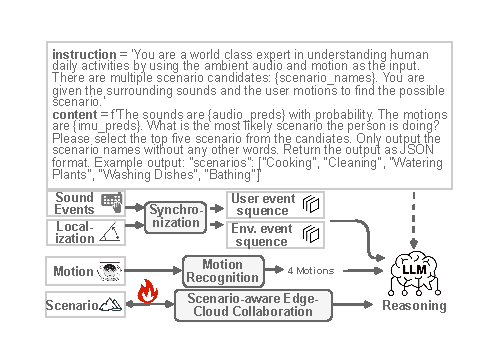
\includegraphics[width=1\linewidth]{chapters/egolog/figs/llm_reasoning.pdf}
\vspace{-2em}
    \caption{LLM-assisted scenario recognition: Utilizing prior outputs, we differentiate sound events into those originating from the user and those from the environment. We then combine it with motion and scenario recognition results and feed it into an LLM for reasoning (the upstream process). The LLM's output is then used as a pseudo-label to re-train the local model (the downstream process).}
    \vspace{-1em}
    \label{fig:egolog_llm_reasoning}
\end{figure}


As discussed in Section~\ref{sec:egolog_measurement}, LLMs may be suboptimal for direct activity recognition. They are better suited to higher-level scenario recognition, where longer data sequences provide richer context. This is consistent with Section~\ref{sec:egolog_scenario}, where longer sequences also benefit multimodal fusion. As illustrated in Fig.~\ref{fig:egolog_llm_reasoning}, EgoLog formats five-second sensor windows as text and uses tailored prompts to guide LLM-based scenario recognition. The LLM output can then refine local scenario predictions. All LLM processing is performed in the cloud so that the local EgoLog model remains lightweight.
 
\subsubsection{Prompt design}
Existing studies primarily use LLM reasoning on text-like data. This subsection introduces how EgoLog converts multimodal audio and motion signals into prompts for LLM-based scenario reasoning, as illustrated in Fig.~\ref{fig:egolog_llm_reasoning}. Instead of retraining the LLM or adding an adapter, EgoLog uses a specialized prompt with demonstrations that describe how to reason over sensor-derived context.
The prompt is structured as follows: “You are an expert in human activity analysis. You will receive audio and IMU recognition results, including extra information on potential scenarios. Using this information, reason and refine the person’s scenario. The scenario must be one of the following categories: [List of categories]. Your output must be a single line containing just one word or phrase.”
This prompt, along with the formatted input data as shown below, is fed to the LLM.

\paragraph{Audio.} 
We employ a pre-trained audio recognizer \citep{schmid2023efficient} to transcribe audio into text by selecting the top three predictions. The output is structured as "the detected audio classes are <class1, prob1>, <class2, prob2>, <class3, prob3>...", where each entry is referred to as a sound event. To minimize noise, we retain only the top five predictions with a confidence score exceeding 0.3.
Since the classifier's label set is based on the AudioSet ontology, the defined classes are highly fine-grained, often resulting in multiple similar classes with comparable probabilities. This lack of discriminative power hinders effective reasoning. To address this, we apply a two-level hierarchical clustering of the classes to their parent categories, reducing the total number of classes from 416 to 50 and improving generalization.

\paragraph{IMU.} 
Following the IMUCLIP approach \citep{moon2023imu2clip}, we classify IMU data into four activities: walking, moving, standing up, and sitting down. While previous works have demonstrated the ability to recognize more fine-grained activities using IMU data, their generalization capabilities remain questionable due to reliance on scenario-constrained datasets.

\paragraph{Spatial.}
EgoLog uses spatial information from Sec.~\ref{sec:egolog_localization} by applying different processing strategies to near-field and far-field audio inputs. For near-field sounds, the prompt states that the sound event occurs near the front of the user and is likely related to human activity. For far-field sounds, the prompt states that the sound event occurs at the estimated sound location.
When both near-field and far-field sounds are detected, it is unclear which event is near or far. As a result, we can turn on the distance-based sound separation \citep{chen2024hearable} that separate the audio into two and perform the sound recognition, respectively. We leave the optimization of the separation in the future work since it is unrelated to the main body of EgoLog.




\subsubsection{Scenario-aware LLM Assistance}

We define an upstream and downstream collaboration paradigm where the edge device seeks assistance from a cloud-based LLM, rather than naively querying the response.

For the upstream path, EgoLog uses the scenario recognition capability of LLMs, especially for out-of-domain data. The scenario estimated by the edge device is treated as a noisy reference that provides preliminary information to the LLM. The prompt includes this estimate and its confidence score.
Specifically, the estimated scenarios are added to the prompt, augmented by the text: "the preliminary scenario estimation is <scenario, confidence>."
However, frequent queries to the cloud service raise concerns about cost, privacy, and latency. Ideally, all modules of EgoLog should be executable on a mobile device if the performance is sufficient. Consequently, we propose a collaborative framework that strategically uses the cloud LLM to enhance the local model. Specifically, a confidence threshold (0.5) is set for the local scenario recognition model. A cloud query is triggered only when the local model's confidence is low.

Complementing the upstream process, we also propose a downstream collaboration where the cloud LLM's output can assist the local model. EgoLog sends the derived textual representation of an uncertain case, rather than its raw audio or IMU samples, to the LLM. The corresponding local sample and the LLM's refined label are then cached on the local device and used to fine-tune the local model, enabling continuous on-device improvement.
Within the scope of EgoLog, we do not consider adding new class to the local model since the required data can be huge, which leads to a long time for waiting.



\section{Evaluation}
\label{sec:egolog_evaluation}
\subsection{Experiment Setup}

\subsubsection{Implementation}
We implemented our system on a Raspberry Pi 4, which was connected to multiple devices: binaural earables (MU6 \citep{Mu6_Home_Page_2020} and Sound Professionals \citep{soundprofessionals}), headphones, and smartglasses. These devices support multi-channel audio recording. Due to the lack of a commercial open platform with the same functionality, we prototyped our system using a 3D-printed model and a configurable microphone array, where the headphone prototype support 4-channel recording and the smart glasses support 4-channel, all devices are shown in Fig. \ref{fig:egolog_device}.
An IMU with a sampling rate of 200 Hz was attached to both the earables and the smartglasses.
The neural network was trained on a server equipped with an Intel i7-11700k CPU and two Nvidia RTX 3090 GPUs using PyTorch. For inference, all computational tasks—except for summary generation—are performed on the smartphone.

\begin{figure}[h]
    \centering
    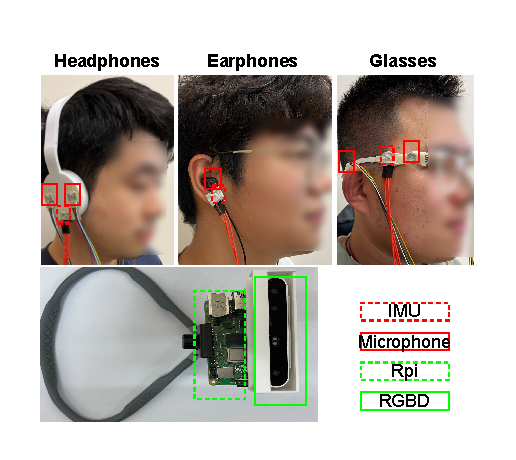
\includegraphics[width=1\linewidth]{chapters/egolog/figs/device.pdf}
    \vspace{-2em}
    \caption{Devices used in our data collection.}
    \vspace{-1em}
    \label{fig:egolog_device}
\end{figure}

\subsubsection{Public dataset}
To comprehensively evaluate EgoLog performance, we construct our dataset with the blow public datasets:

\paragraph{Ego4D:}
Ego4D \citep{grauman2022ego4d} is a large-scale dataset collected by various brands of head-mounted cameras (e.g., GoPro), offering synchronized multi-modal data (i.e., video, audio, and IMU signal). We consider the moment subset of the dataset, which consists of 158 classes. We can perform k-means clustering on the text embeddings to adapt to different levels of granularity. For the scenario annotation, we use the scenario annotation \citep{grauman2022ego4d} for each video since they have a similar definition. In total, there are 91 scenarios in the dataset. 
Considering Ego4D is the most diverse and large-scale dataset, we set it as the default dataset.

\paragraph{EgoADL:}
EgoADL \citep{sun2024multimodal} is also a large-scale dataset collected in the real world with Android smartphones, including Wi-Fi, audio, and IMU data. In this paper, we exclude Wi-Fi data for fair comparison. We perform a similar clustering for the 221 classes of actions in the dataset.

\paragraph{SAMOSA:}
SAMOSA \citep{mollyn2022samosa} is a relatively small-scale dataset collected by an Android smartwatch (i.e., Fossil Gen 5), including audio and IMU. There are 26 activities in total.

\subsubsection{Self-collected dataset}
The existing public datasets already include data from various devices—such as smart glasses, smartphones, and smartwatches—offering considerable duration and diversity. The purpose of our self-collected dataset is not to surpass these strengths but to address their limitations. Specifically, the spatial understanding discussed in Section \ref{sec:egolog_localization} relies on spatial audio, which is absent from the aforementioned datasets but is accessible using commercial devices. To compensate for this gap, we collected a new dataset featuring spatial audio recordings from different form factors: glasses, headphones, and earphones.

We constructed a dataset in which a volunteer acted as the user and a loudspeaker served as an audio interference source. The loudspeaker played audio samples from the NIGENS dataset \citep{trowitzsch2019nigens}, which contains 14 types of common sound events. The user, in contrast, performed the following 12 activities: standing up, sitting down, clapping, walking, talking, drinking, typing on a keyboard, eating, watching TV, washing hands, cleaning a room, and writing.
During data collection, the loudspeaker's position remained fixed. To simplify the experiment, the user's location was controlled for most activities (excluding walking), allowing us to manually record the relative position between the user and the loudspeaker. However, as users were not required to remain perfectly still, their precise position was not controlled with high accuracy. To ensure the dataset's validity, users were instructed to limit their positional variance to within the spatial resolution of our classification model. In essence, while the user's location was dynamic, the annotation was treated as static from the perspective of the classification task.
For the walking activity, where the relative position changes continuously, we used an RGB-D camera to perform Simultaneous Localization and Mapping (SLAM) to estimate the user's trajectory. This estimation was based on the assumption that the user started from a fixed, known position in the room (the location of the loudspeaker is also fixed and known).


\subsubsection{Baselines}
We adopt the following evaluation metrics in this paper. For the multi-label classification (i.e., scenario and spatial), we use the multi-label F1-Score: $2*TP/(2*TP+FP+FN)$. For the single-label classification (i.e., activity), we use the accuracy as the metric.

To evaluate our approach, EgoLog, we have selected different baselines for activity recognition and scenario recognition, respectively. Specifically, we consider SAMoSA \citep{mollyn2022samosa} and Imagebind \citep{girdhar2023imagebind} as our baselines for activity recognition, which are conventional supervised multi-modal model that accepts both audio and IMU. For the scenario recognition, both of the above baselines with larger data duration are considered. To ensure a fair comparison, all of them are fine-tuned with the same data.

\subsection{Activity Recognition}
\begin{figure}[h]
    \centering
    \begin{minipage}{0.48\linewidth}
        \centering
      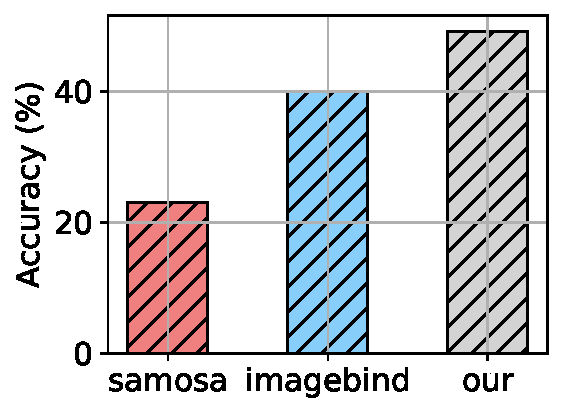
\includegraphics[width=1\linewidth]{chapters/egolog/eval/activity_ego4d.pdf}
          \vspace{-0.5em}
      \caption{Activity recognition on Ego4D.}
        \label{fig:egolog_activity_ego4d}
    \end{minipage}
    \hfill
    \begin{minipage}{0.48\linewidth}
        \centering
    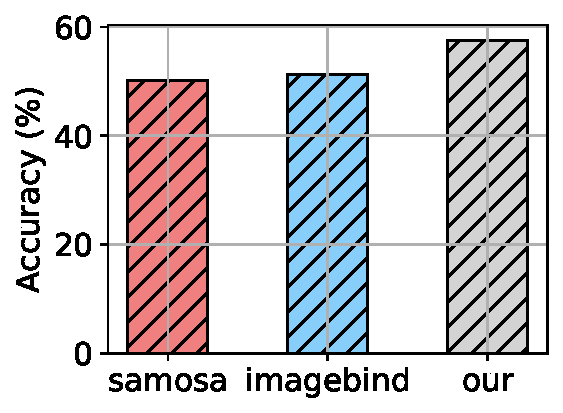
\includegraphics[width=1\linewidth]{chapters/egolog/eval/activity_egoadl.pdf}
        \vspace{-0.5em}
      \caption{Activity recognition on EgoADL.}
        \label{fig:egolog_activity_egoadl}
    \end{minipage}
    \vspace{-0.5em}
\end{figure}

\begin{figure}[h]
    \centering
    \begin{minipage}{0.48\linewidth}
        \centering
       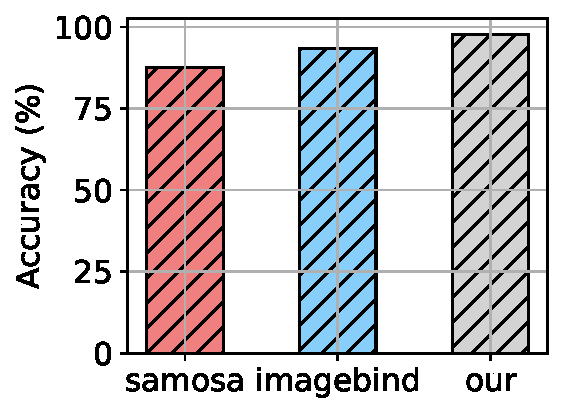
\includegraphics[width=1\linewidth]{chapters/egolog/eval/activity_samosa.pdf}
           \vspace{-0.5em}
      \caption{Activity recognition on SAMOSA.}
        \label{fig:egolog_activity_samosa}
    \end{minipage}
    \hfill
    \begin{minipage}{0.48\linewidth}
        \centering
    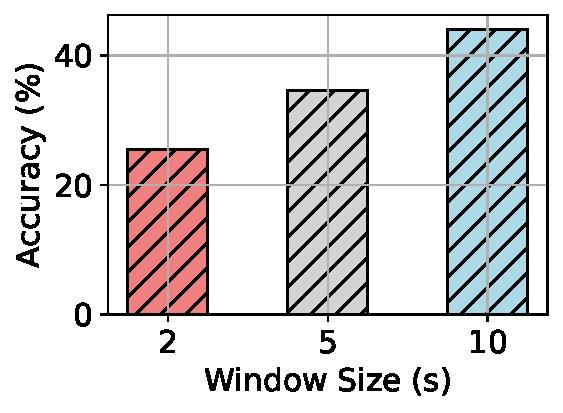
\includegraphics[width=1\linewidth]{chapters/egolog/eval/activity_window_size.pdf}
        \vspace{-0.5em}
      \caption{Activity recognition vs. data length.}
        \label{fig:egolog_activity_length}
    \end{minipage}
\vspace{-0.5em}
\end{figure}

We present the performance of our method for human activity recognition on the Ego4D, EgoADL, and SAMOSA datasets. As shown in Fig. \ref{fig:egolog_activity_ego4d}, \ref{fig:egolog_activity_egoadl}, and \ref{fig:egolog_activity_samosa}, our approach consistently outperforms the baselines, with the most notable improvement on the SAMOSA dataset.

The performance gap is most significant on the Ego4D dataset (23\% vs. 52\%), which is the most challenging. Compared to ImageBind, EgoLog achieves superior performance (52\% vs. 40\%) with significantly lower computational cost.

On the other two, less diverse datasets, the advantages of EgoLog are slightly reduced. We attribute this primarily to a lack of contextual information; Ego4D data was collected "in the wild," while the others were gathered in moderately controlled experimental settings. Despite this, our approach still outperforms the best baseline by 6\%on EgoADL and 4\%on SAMOSA, demonstrating its robustness. Note that the absolute accuracy for SAMOSA is the highest, which is expected as it has the smallest number of classes, making it the least challenging dataset.


\paragraph{Data length.}
Since the length of the data significantly influences both audio and IMU data, we first establish the hyperparameters before evaluating the system.
We present the performance of human activity recognition along with various data lengths, in Fig. \ref{fig:egolog_activity_length}. We observe that the HAR performance stays stable when the data length is larger than five seconds, while significantly dropping when the data length is one second. As a result, we keep the data length of HAR to five seconds. 

\begin{figure}[h]
    \centering
    \begin{minipage}{0.48\linewidth}
        \centering
       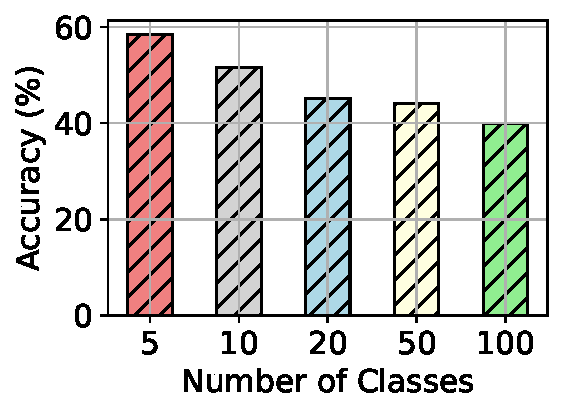
\includegraphics[width=1\linewidth]{chapters/egolog/eval/activity_num_classes.pdf}
           \vspace{-0.5em}
      \caption{Human activities recognition performance vs. number of classes.}
        \label{fig:egolog_activity_num_classes}
    \end{minipage}
    \hfill
    \begin{minipage}{0.48\linewidth}
        \centering
    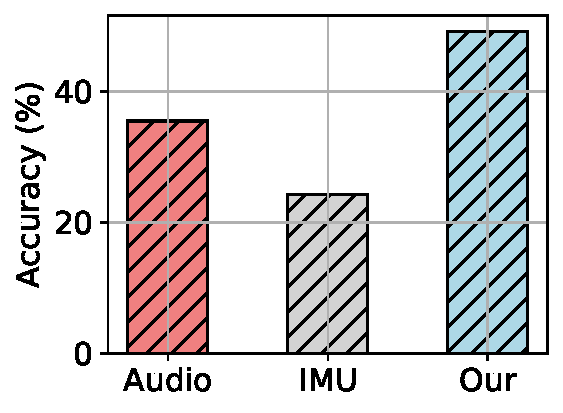
\includegraphics[width=1\linewidth]{chapters/egolog/eval/activity_modality.pdf}
        \vspace{-0.5em}
      \caption{Human activities recognition performance vs. modality.}
        \label{fig:egolog_activity_modality}
    \end{minipage}
\vspace{-0.5em}
\end{figure}

\paragraph{Number of classes.}
We split the sampled Ego4D dataset into activities and evaluated their performance in Fig. \ref{fig:egolog_activity_num_classes}. We observe that there are performance gaps between activities, indicating that the complexity of each of them is different. Specifically, we inspect the top three worst activities, which are putting something in a container or on a surface, cutting with scissors, and sleeping. We observe that they are both quiet, and the motion is weakly related to the head, so it is natural to have lower performance.

\paragraph{Modalities fusion.}
As shown in Figure \ref{fig:egolog_activity_modality}, our multi-modal fusion approach (audio+IMU) surpasses the audio-only and IMU-only baselines, improving activity recognition performance by more than 10\%.


\begin{table}[h]
\centering
\caption{Ablation study on activity recognition for different datasets, the metric is accuracy.}
\label{tab:ab_activity}
\begin{tabular}{ccccc}
\toprule
\textbf{Model}  & \textbf{Ego4D$\uparrow$} & \textbf{EgoADL$\uparrow$} & \textbf{SAMOSA$\uparrow$} \\
\midrule
Random  & 0.02 & 0.02 & 0.04 \\
\midrule
ImageBind-FT  & 0.40 & 0.51 & 0.93 \\
\midrule
Multi-modal & 0.401 & 0.49 & 0.90\\
+ Scenario & \textbf{0.467} & \textbf{0.58} & \textbf{0.97} \\
\bottomrule
\end{tabular}
\end{table}

\paragraph{Ablation study.}
We conduct an ablation study on different components of our system, including each modality (audio and IMU), multi-modal fusion, scenario as condition, and scenario as condition via Imagebind-embedding, as shown in Tab. \ref{tab:ab_activity}. For reference, we also list the performance of a random guess (indicating the number of classes) and baseline ImageBind-FT.
We observe that


\subsection{Scenario Recognition}
\begin{figure}[h]
    \centering
    \begin{minipage}{0.48\linewidth}
        \centering
    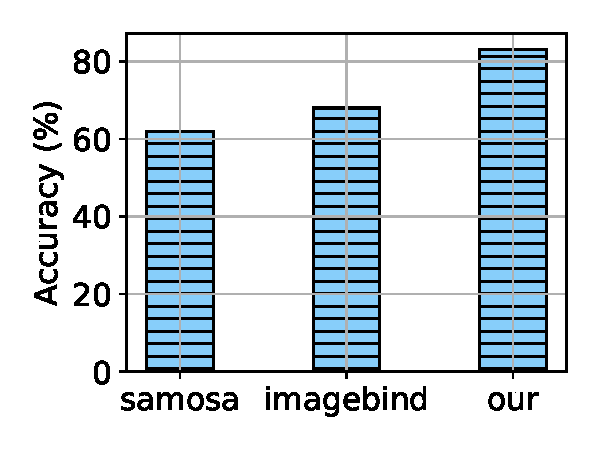
\includegraphics[width=1\linewidth]{chapters/egolog/eval/scenario_cls.pdf}
           \vspace{-0.5em}
      \caption{Scenario recognition accuracy on Ego4D.}
        \label{fig:egolog_scenario}
    \end{minipage}
    \hfill
    \begin{minipage}{0.48\linewidth}
        \centering
    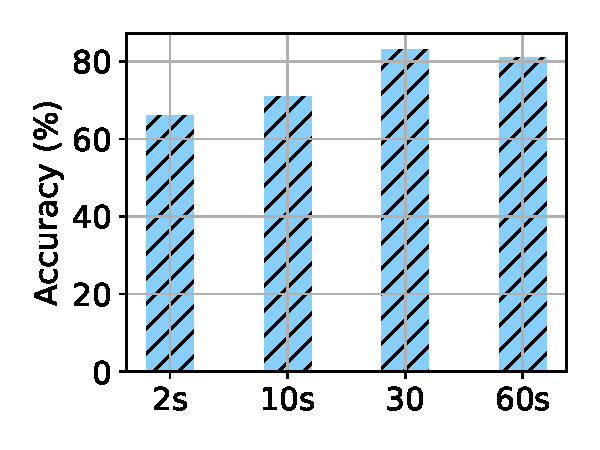
\includegraphics[width=1\linewidth]{chapters/egolog/eval/scenario_length.pdf}
        \vspace{-0.5em}
      \caption{Scenario recognition accuracy vs. data length.}
        \label{fig:egolog_scenario_length}
    \end{minipage}
    \vspace{-0.5em}
\end{figure}



\begin{figure}[h]
    \centering
    \begin{minipage}{0.48\linewidth}
        \centering
      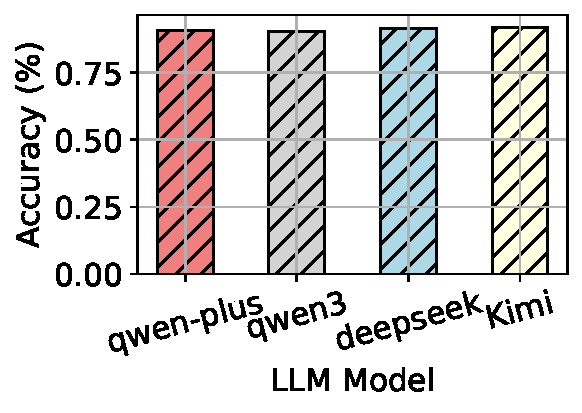
\includegraphics[width=\linewidth]{chapters/egolog/eval/scenario_llm_model.pdf}
          \vspace{-0.5em}
     \caption{Selection of LLM.}
    \label{fig:egolog_selection_llm}
    \end{minipage}
    \hfill
    \begin{minipage}{0.48\linewidth}
     \begin{tabular}{cc}
        \toprule
        \textbf{Model} & \textbf{Ego4D$\uparrow$} \\
        \midrule
        Random & 0.01\\
        \midrule
        Multi-modal & 0.70 \\
        + Contrastive & 0.83\\
        + Transformer  & 0.85 \\
        + LLM feedback  & 0.90\\
        \bottomrule
        \end{tabular}
        \vspace{1em}
        \captionof{table}{Ablation study on scenario recognition.}
        \label{tab:ab_scenario}
    \end{minipage}
    \vspace{-0.5em}
\end{figure}


Recalled in Sec. \ref{sec:egolog_scenario}, we employ a two-stage model to recognize the scenario by extracting the key-frame. In comparison, we consider audio scene recognition and ImageBind-IMU, which are audio-only and IMU-only methods
as the two baselines shown in Fig. \ref{fig:egolog_scenario}. We observe that our method outperforms the two baselines by 15\%, indicating that our long-time multi-modal fusion works well for scenario recognition. 

\paragraph{Data length.}
Based on our earlier definitions, scenarios that require capturing long-term information should use longer data lengths. We present the performance of scenario recognition along with various data lengths in Fig. \ref{fig:egolog_scenario_length}. We observe that the ideal data length is set to 30 seconds since the larger input data can reduce the performance.

\paragraph{Selection of LLM.}
Since our design is compatible with any LLM, we evaluated the performance using different LLMs from various sources. As shown in Fig. \ref{fig:egolog_selection_llm}, we observe that the performance is similar across them, indicating that common LLMs are sufficient for our design. For better deployment, we plan to explore the use of smaller LLMs in the future to reduce costs.

\paragraph{Ablation study.}
We conducted an ablation study to evaluate the contribution of different components in our system, including contrastive learning, the transformer module, and the addition of LLM feedback. The results are presented in Tab. \ref{tab:ab_scenario}. For reference, we also include the performance of a random guess (based on the number of classes).

Our observations indicate that contrastive learning is the most effective component, providing the largest performance improvement (13\%). The LLM feedback, facilitated by edge-cloud collaboration, yields a further, albeit smaller, gain. Given that LLM feedback is less susceptible to cross-domain variations, we consider this slight improvement to be meaningful.



\subsection{Spatial Understanding for Scenario Recognition}
\begin{figure}[h]
    \centering
    \begin{minipage}{0.48\linewidth}
         \centering
    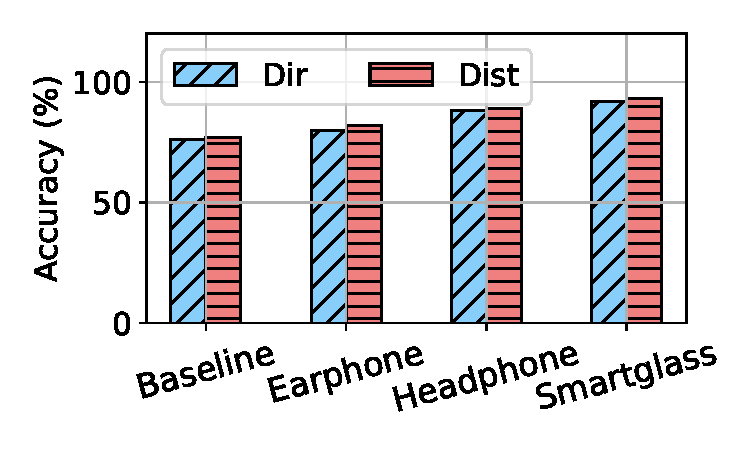
\includegraphics[width=1\linewidth]{chapters/egolog/eval/sound_localization.pdf}
            \vspace{-0.5em}
      \caption{Sound localization accuracy.}
        \label{fig:egolog_sound_localization}
    \end{minipage}
    \hfill
    \begin{minipage}{0.48\linewidth}
        \centering
    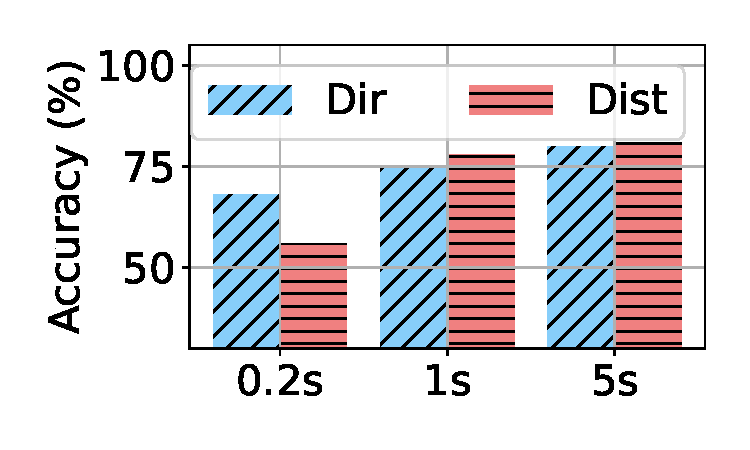
\includegraphics[width=1\linewidth]{chapters/egolog/eval/sound_localization_length.pdf}
          \vspace{-0.5em}
    \caption{Sound localization accuracy vs. data length.}
    \label{fig:egolog_sound_localization_length}
    \end{minipage}
    \vspace{-0.5em}
\end{figure}

\begin{figure}[h]
  \centering
  \begin{minipage}{0.4\linewidth}
    \centering
    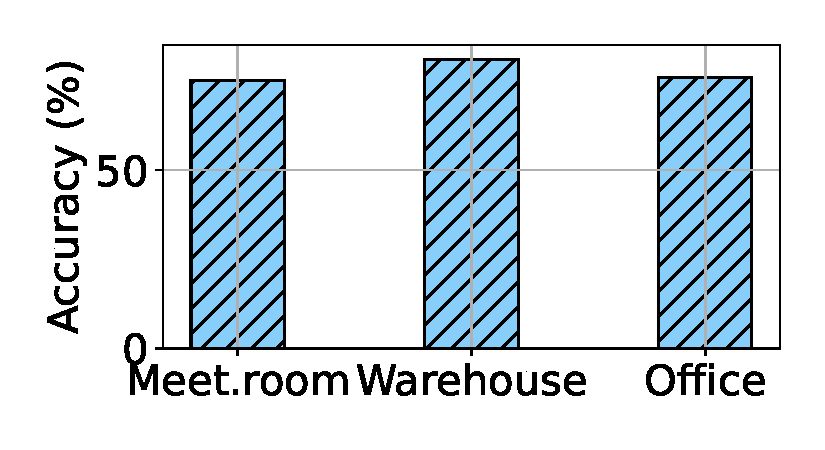
\includegraphics[width=1\linewidth]{chapters/egolog/eval/sound_localization_place.pdf}
        \vspace{-0.5em}
      \caption{Sound localization accuracy at different places.}
        \label{fig:egolog_sound_localization_place}
  \end{minipage}
  \hfill
  \begin{minipage}{0.58\linewidth}
    \centering
     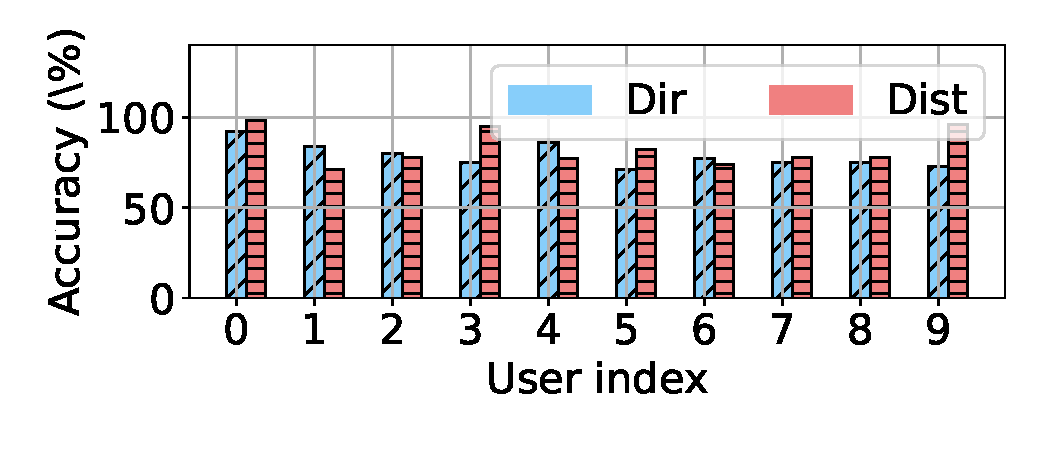
\includegraphics[width=1\linewidth]{chapters/egolog/eval/sound_localization_user.pdf}
         \vspace{-0.5em}
      \caption{Binaural sound localization accuracy for different users.}
        \label{fig:egolog_sound_localization_user}
  \end{minipage}
\vspace{-0.5em}
\end{figure}
In Fig. \ref{fig:egolog_sound_localization}, we compare the baseline (without motion compensation) with our proposed method across different devices. We report the accuracy for both direction (Dir) and distance (Dist) separately. The results show that our method improves accuracy by approximately 10\%when using IMU data for motion compensation.

Regarding performance across devices, we observe a consistent improvement from binaural earphones to 4-channel headphones and further to 4-channel smart glasses, which aligns with our expectations. In the following section, we will focus on evaluating data from earphones, which exhibit the lowest performance.

\paragraph{Data length.}
Since the length of the audio significantly influences the performance of sound localization, we test the accuracy with different length of data in Fig. \ref{fig:egolog_sound_localization_length}. According to the result, we set the data length of sound localization to one second to balance the latency and accuracy.

\paragraph{Different environments.}
We conducted further assessments of localization accuracy across various environments, such as distinct rooms. Room layout and object configurations induce varying room impulse responses, affecting recordings in conjunction with HRTFs. Our performance evaluation across different rooms is presented in Figure \ref{fig:egolog_sound_localization_place}, demonstrating that our model maintains consistent performance across diverse settings.

\paragraph{Different users.}
Binaural sound localization depends on individual-specific HRTFs, rendering neural networks calibrated for one user
ineffective for others. We assess personalized models across a group of users and present the overall accuracy in Figure 21. Despite performance variations among users, consistent accuracy (>75\%) is maintained within the group

\subsection{User Study}

% \begin{table}[h]
% \centering
% \vspace{-0.5em}
% \caption{User study.}
% \label{tab:user_study}
% \begin{tabular}{ll}
% \toprule
% \textbf{Question} & \textbf{EgoLog}\\
% \midrule
% Correctness &  \\
% Information-richness & \\
% User-friendly & \\
% \bottomrule
% \end{tabular}
% \vspace{-0.5em}
% \end{table}

To evaluate the benefits of EgoLog from a user perspective, we conducted a study where volunteers provided subjective ratings of the system's outputs. Recall that our goal is to provide users with a daily log that comprehensively summarizes and represents their activities through two complementary types of output: scenarios and activities. 
Our final solution integrates both outputs: the daily log displays two rows, with the first row showing scenario information and the second row presenting activity data. Since scenarios are recognized every 30 seconds, the output can contain errors or inconsistencies, even within the same scenario. To mitigate this, we represent each scenario using the normalized probability calculated from the most recent 10 minutes of data. 
For activities, due to the larger volume of data, we present the results using a bar chart with activity names labeled at the bottom.
Users were asked to rate the outputs based on three criteria: Correctness, Information-richness, and User-friendliness. To assess correctness, they were provided with ground-truth data in the same format. The average ratings (on a scale of 1-min to 5-max) for the three dimensions were 4.5, 4.0, and 4.5, respectively.


\subsection{Overhead}
While our system is not specifically designed for real-time responses, it is crucial to maintain low resource consumption.

\begin{table}[h]
\centering
\vspace{-0.5em}
\caption{Model runtime latency.}
\vspace{-0.5em}
\label{tab:latency}
\begin{tabular}{llcc}
\toprule
\textbf{Section} & \textbf{Interval} & \textbf{CPU} & \textbf{GPU} \\
\midrule
Scenario & 30 seconds & 0.55s & 9ms \\
Spatial & 2 seconds & 2.5ms & 2.1ms \\
HAR  & 10 seconds & 34ms & 2.7ms \\
\bottomrule
\end{tabular}
\vspace{-0.5em}
\end{table}

\paragraph{Latency.}
EgoLog comprises three core components: (1) scenario recognition (Sec. \ref{sec:egolog_scenario}), (2) sound localization (Sec. \ref{sec:egolog_localization}), and (3) HAR (Sec. \ref{sec:egolog_har}). As shown in Tab. \ref{tab:latency}, most components are lightweight, enabling real-time performance on both CPU and GPU platforms. Notably, scenario recognition on CPU requires 0.55 seconds but is executed once every 30 seconds, rendering its latency negligible. While EgoLog does not mandate real-time user feedback, lower latency enhances user experience by minimizing wait times.


\paragraph{Power consumption.}
To evaluate our power consumption, we locked the screen while continuously recording both audio and IMU data. We then checked the battery level before and after one hour of recording. Using the Pixel 7 as a reference, we observed approximately a 5\% drop in power after one hour of recording. Given that there is potential for further optimization, EgoLog shows promise for effective long-term operation.

\paragraph{Data storage.}
We record audio at a sample rate of 48 kHz, with a 16-bit depth and 2 channels, resulting in a compressed file size of about 170-210 kbps in MP3 format. This equates to around 70 MB of audio data per hour. For motion data, with an update rate set to 10 Hz, the size in CSV format is approximately 1 kB per second, leading to around 3 MB of data per hour.
As a result, we can process this data periodically, ensuring that storage requirements remain manageable and do not become overwhelming.





The system's privacy boundary and deployment safeguards are discussed in Section~\ref{sec:thesis_privacy}.


\chapter{CoHear: Conversation Enhancement via Multi-Earphone Collaboration}\label{ch:cohear}
The chapter presents CoHear, a novel cooperative hearing system that leverages multiple devices to enhance audio perception in challenging environments. We discuss the system architecture, implementation details, and evaluate its performance through extensive experiments.

\section{Introduction}

\begin{figure}
    \centering
    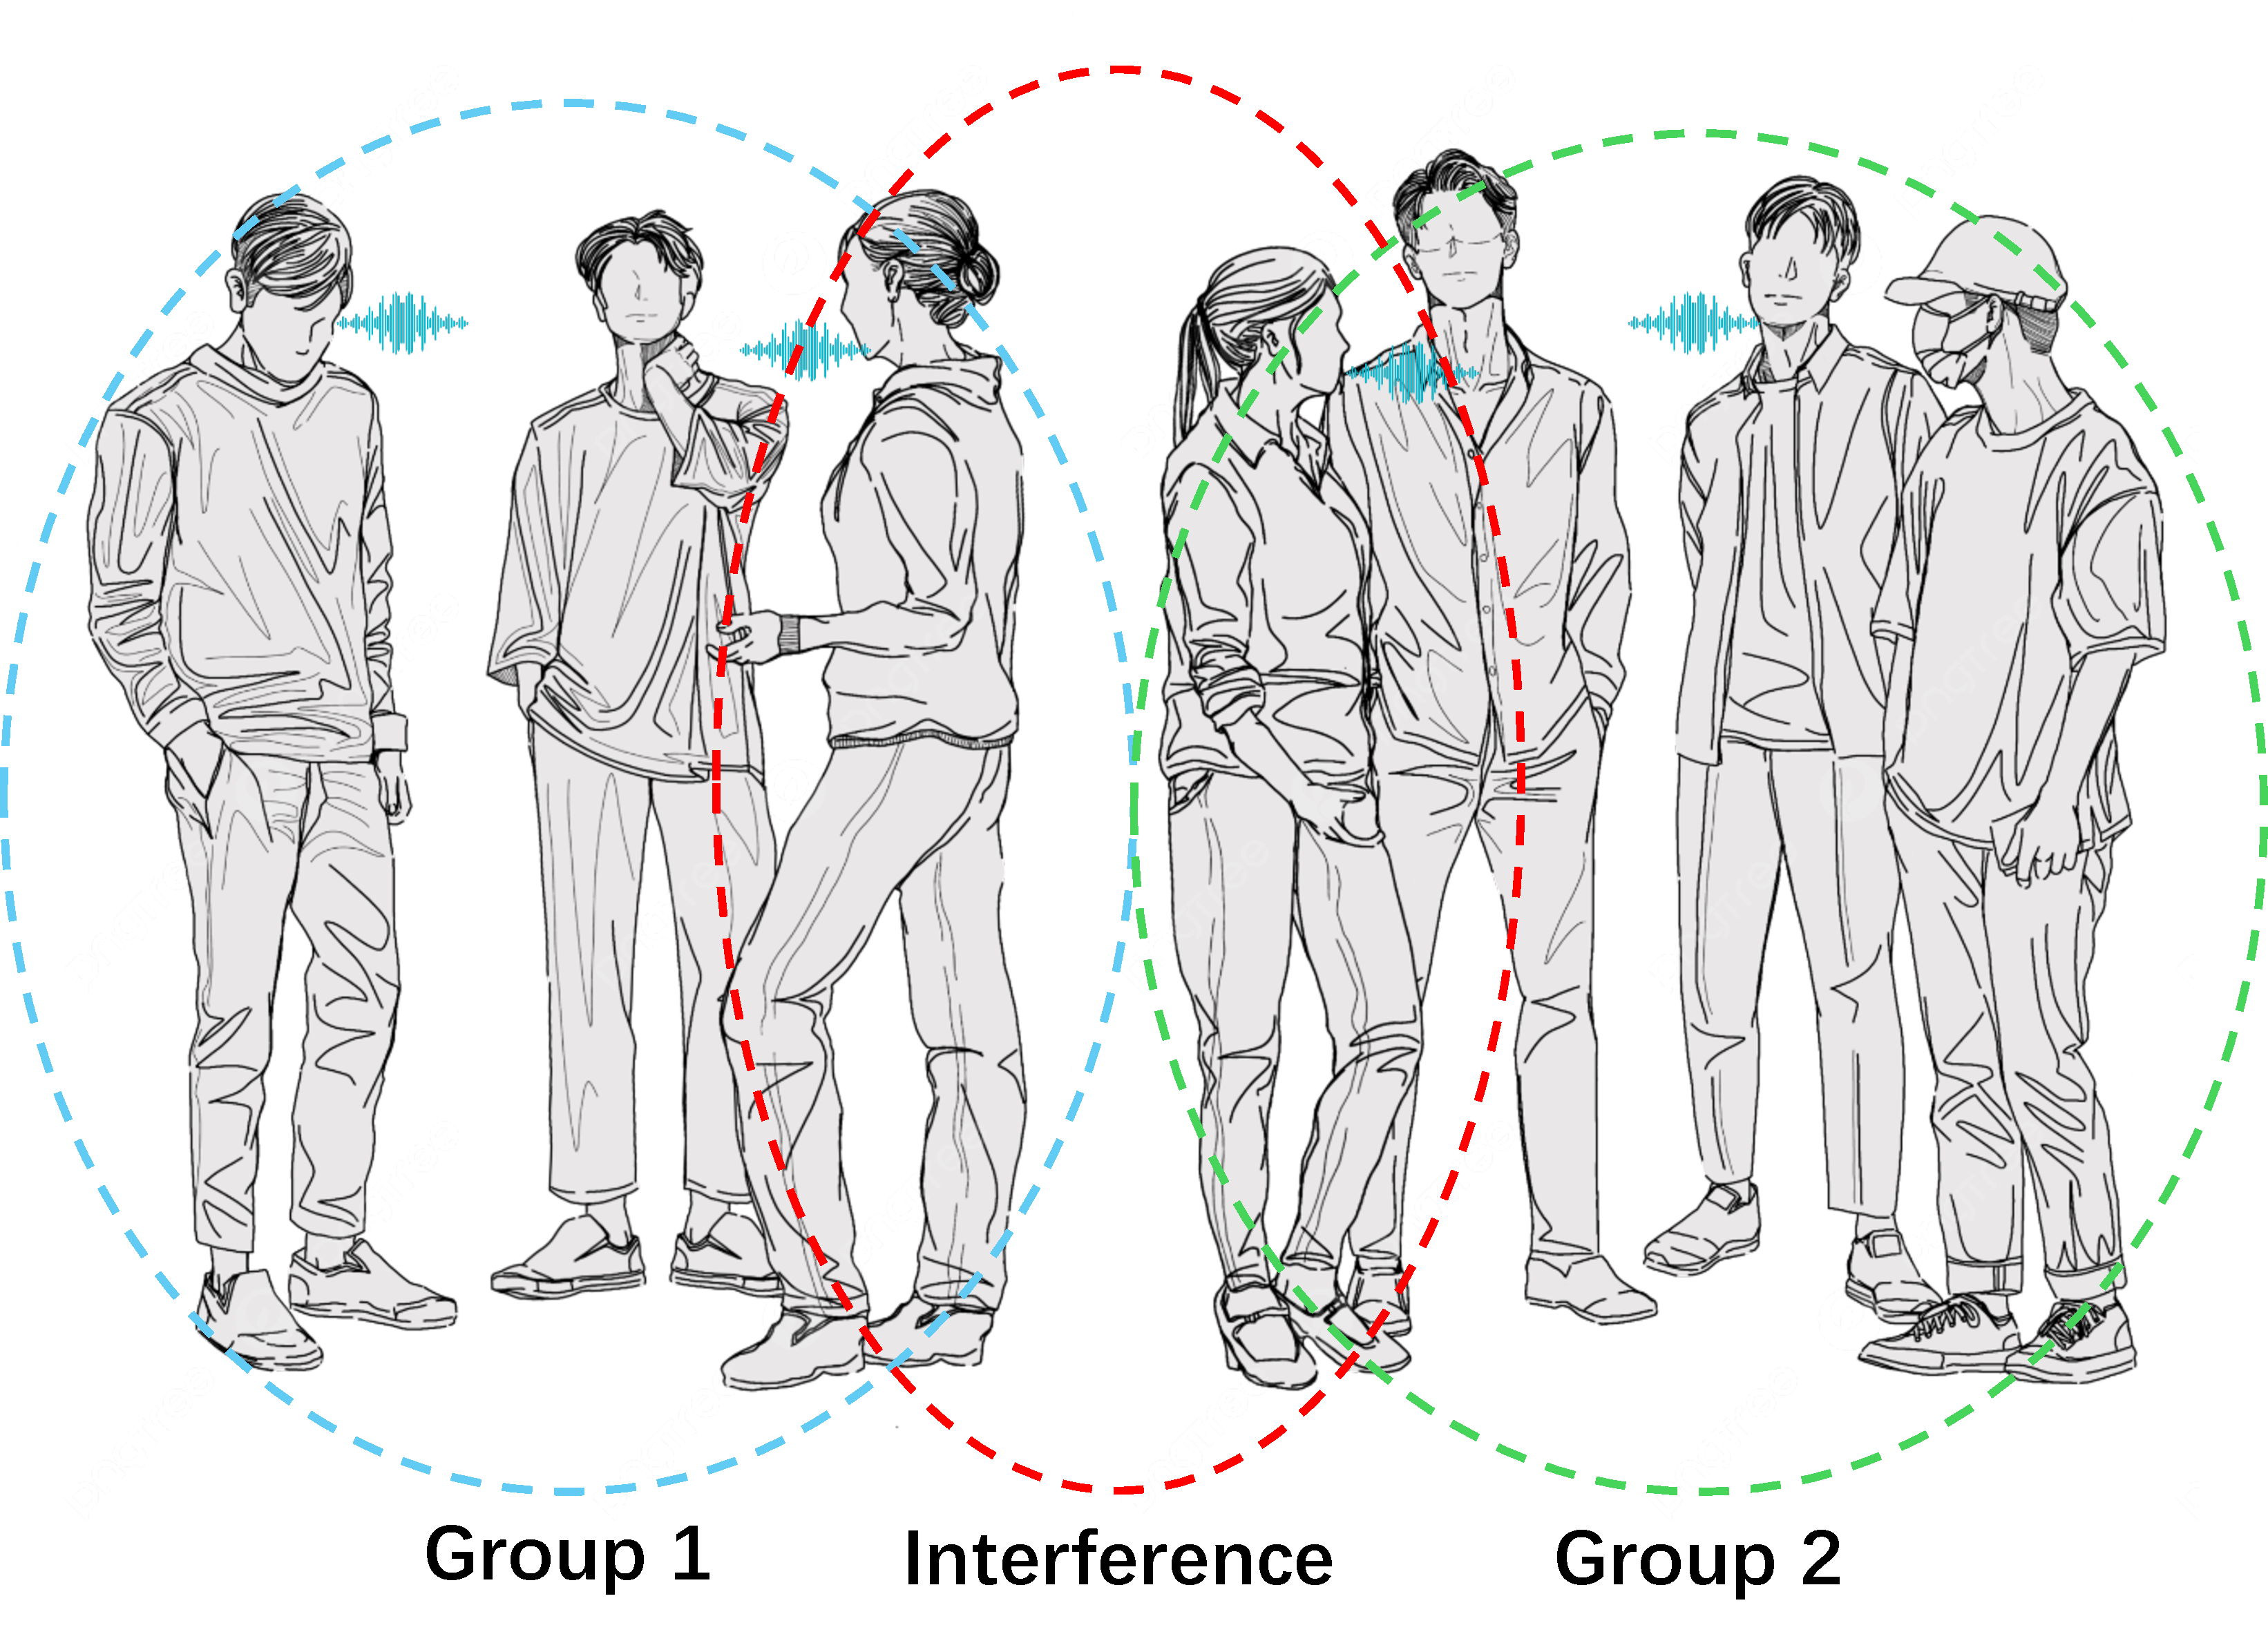
\includegraphics[width=0.6\linewidth]{chapters/cohear/figs/illustration.pdf}
    \vspace{-1em}
    \caption{CoHear uses natural conversational interaction to discover conversation partners and enhance speech within the same conversation group.}
    \label{fig:illustration}
    \vspace{-1em}
\end{figure}

Smart earphones have become a widely deployed wearable platform, with approximately 455 million units shipped globally in 2024 and 11.2\% year-on-year growth~\cite{patentlyapple2025audio}.
Beyond music playback, recent earphone systems support speech enhancement~\cite{chatterjee2022clearbuds, he2023towards, duan2024earse}, speech anti-tampering~\cite{duan2024f2key, hearid}, fine-grained activity recognition~\cite{lyu2024earda}, and spatial audio through IMU-based head tracking~\cite{han2023headmon, han2023headsense, lyu2024earda}. These capabilities make earphones suitable for conversation sensing because they capture both verbal signals and non-verbal cues such as head orientation.

Conversation is an interactive form of communication between two or more people and plays a crucial role in socialization. As illustrated in Fig.~\ref{fig:illustration}, people naturally form separate conversation groups, and ideally, each person wants to focus solely on the members of their own group, regardless of distance or competing voices. The ``cocktail party effect'' \cite{pollack1957cocktail} refers to the human ability to selectively concentrate on a particular voice in noisy environments. However, this perceptual mechanism has limitations. Many individuals experience what is known as ``cocktail party deafness,'' which hinders their ability to follow conversations in crowded settings due to hearing impairments, cognitive overload, or overwhelming background noise \cite{pryse2009companion, cherry1953some}. As a result, clear communication in environments such as conferences, networking events, or guided tours becomes increasingly challenging.


Earphones can therefore serve as assistive tools for conversation listening. However, existing speech enhancement methods do not fully model conversational context. Some methods enhance hearing based on sound categories~\cite{veluri2023semantic}, speaker recognition~\cite{veluri2024look}, or listener distance~\cite{chen2024hearable}, but these cues do not always capture the dynamics of natural conversation. SoundBubble~\cite{chen2024hearable}, for example, assumes a defined spatial region, while real conversations may form across irregular distances and orientations. The method in~\cite{chen2024target} extracts conversations based on turn-taking dynamics and previously recorded audio, but its reliance on turn-taking events introduces delay and limits real-time use.


To address these limitations, CoHear uses multi-device collaboration for conversation enhancement. In contrast to earphone systems that focus on single-device processing~\cite{dong2024rehearsse, he2023towards, duan2024earse}, CoHear treats conversation as a multi-user activity. It connects individual earphones into a lightweight network and combines wearable sensing with distributed acoustic observations.


The CoHear earphone network departs from the conventional assumptions of wireless acoustic sensor networks in two ways~\cite{gburrek2021geometry}. Traditionally, such networks assume that (1) sound sources appear randomly and independently of sensor node placement, and (2) the sensor nodes themselves remain static. In contrast, the conversation-driven setting has a different structure: the sound sources, i.e., human speakers, are co-located with mobile sensor nodes (earphones), and these nodes dynamically organize themselves into conversation groups, as illustrated in Fig.~\ref{fig:illustration}.
Consequently, the conversation network is triggered and constructed by interactions among users, which can be modeled through verbal or non-verbal features. Verbal features such as turn-taking are delayed and sensitive to interference, so CoHear primarily uses non-verbal features such as head orientation to infer conversation groups.

To establish the conversation network, CoHear uses multi-channel audio and IMU recordings to detect nearby speakers, estimate their locations, and infer conversations from relative orientations. The enhanced speech can then be rendered through noise-canceling earphones. Implementing this system raises three challenges:
\begin{itemize}
    \item \textbf{Dynamic peer discovery and network formation.} Since conversations occur spontaneously and participants are mobile, the system must continuously identify nearby speakers, localize their positions, and group devices into socially coherent clusters without any fixed infrastructure.

    \item \textbf{Topology estimation and coordination.}
    The estimation and observations of a single user may be insufficient to identify conversation participants. Therefore, aggregating the noisy, distributed observations from heterogeneous devices is necessary for establishing a global coordinate system to locate conversations.

    \item \textbf{Conversation enhancement.}
    Even a well-established conversation network may not be directly useful to users without additional processing. The earphone platform enables targeted extraction of conversation-level speech, but the system must select and use conversation conditions, such as speaker embeddings, from the network under latency and bandwidth constraints.
\end{itemize}



To address these challenges, CoHear makes three contributions:
\begin{enumerate}
    \item \textbf{A conversation network for earphones.}
    CoHear designs a conversation network that uses earphone sensing to model conversation groups without fixed infrastructure. The network includes two components:
    (i) a node discovery module that detects nearby speakers along with their locations and speaker embeddings, as described in Sec. \ref{sec:cohear_acoustic}. This task is divided into two parts: sound source localization and speaker embedding extraction. A joint identity extraction model is used to integrate these two elements.
    (ii) a geometric calibration pipeline that estimates the global network topology using the output from node discovery, as detailed in Sec. \ref{sec:cohear_geometric}. This pipeline matches sound sources identified across different devices, calculates the distances between them, and uses this information for geometric calibration.

    \item \textbf{Bandwidth-aware target conversation enhancement.}
    Based on the network structure, CoHear develops a conversation enhancement module for low latency and bandwidth efficiency. This module uses peer-relayed audio as conditioning signals and remains effective under network delays, packet loss, and compression artifacts. An adaptive model uses both time-invariant and time-varying conditioning features, while an audio control module manages feature selection and bandwidth usage.

    \item \textbf{A practical implementation with real-world validation.}
    CoHear is implemented on earphones equipped with microphones and IMUs. Real-world experiments, simulations, and user studies show over 90\% accuracy in conversation group formation, up to 8.8 dB SNR improvement over representative baselines, and real-time performance (RTF > 1) on mobile devices. An adaptive bandwidth controller further improves performance under constrained conditions.
\end{enumerate}

% \section{Related Work}
\label{sec:related}

\subsection{Conversation Modeling}
Conversation involves the exchange of thoughts, feelings, and ideas between two or more people. A natural conversation is not simply a combination of multiple speeches; it also includes both verbal and non-verbal elements. Modeling conversations has significant technical and social implications.

\paragraph{Non-verbal feature}
Non-verbal features, also known as body language \cite{d2010multimodal}, play a crucial role in conversations. Previous research has explored detecting social interactions using acceleration data from neck-worn sensors \cite{gedik2018detecting}. However, acceleration-based methods are inherently limited to capturing the wearer's own movements and cannot perceive contextual factors or the behaviors of others. Their effectiveness relies on coordinated actions between individuals, which are often inconsistent.

In contrast, vision and audio offer a more direct approach to modeling social interaction. For instance, the Ego4D benchmark defines interaction through the objectives "look at me" and "talk to me" \cite{grauman2022ego4d}. Similarly, multi-modal methods like visual-guided beamforming (e.g., in EasyCom \cite{donley2021easycom}) outperform audio-only approaches by leveraging both data types. However, due to the computational overhead of vision, audio-only solutions remain advantageous. These methods typically work by estimating the speaker's location \cite{wang2022nerc, yang2022deepear}, but this alone is insufficient, as it fails to capture the speaker's orientation—a key component of "talking to me." Some research has aimed to jointly estimate location and orientation \cite{ahuja2020direction}, but these methods are designed for static microphone arrays and lack the adaptability needed for dynamic, real-world environments.

\paragraph{Verbal feature}
In addition to non-verbal cues, the content of speech is also a vital aspect of conversation, as highlighted in \cite{sacks1974simplest}. A closely related task is speaker diarization \cite{bredin2023pyannote}, which identifies "who spoke when" and can further transcribe the corresponding text. By analyzing the conversation content \cite{wei2022conversational}, we can generate meeting summaries \cite{ramprasad2024analyzing} or improve readability \cite{wang2024diarizationlm}. Beyond semantic analysis, the dynamics of turn-taking in conversations are noteworthy, as they exhibit clear temporal patterns and are essential for understanding social interactions \cite{levinson2015timing}. 
Previous studies have attempted to utilize the turn-taking to either proactively mediate the conversation \cite{lee2018flower} or detect the turn-taking events by examining natural overlaps and backchannels \cite{chen2024target, chang2022turn}. However, it is important to note that turn-taking detection is only effective once it has occurred, which means that waiting for enough data can pose a significant delay. 

In summary, non-verbal features are more stable for modeling conversation and introduce less delay than verbal features, making them more suitable for deployment in our system. However, current methods fail to extract these features without visual data, which is unavailable for standard headphones.


\subsection{Acoustic Sensing Systems}
Recent advancements in mobile computing leverage acoustic modalities to enable human-centric applications, laying the groundwork for CoHear. These works can be categorized into two primary areas: single device and multiple devices, by the number of devices utilized in the system.

\paragraph{Single device}
The acoustic sensing capabilities of a single device can be further categorized based on the frequency band utilized. Specifically, when only audible sound (below 20 kHz) is employed, this is referred to as audible acoustic sensing. Conversely, when the ultrasonic frequency band is used, it is classified as ultrasonic acoustic sensing.

Audible acoustic sensing extracts semantic content, such as speech transcription \cite{gao2023funasr} or sound classification \cite{gemmeke2017audio}, or derives spatial information through multi-channel audio recordings \cite{wang2019doa}. However, its applications are constrained to audible sources, making it less versatile in complex environments. In contrast, ultrasonic sensing uses controlled, inaudible sound waves to convey information, supporting a diverse range of tasks: underwater localization and communication \cite{chen2022underwater, chen2023underwater}, backscatter \cite{jang2019underwater}, air-to-water communication \cite{tonolini2018networking}, SOS signal transmission \cite{yang2023aquahelper} and dual-channel communication \cite{qian2021aircode}. Except for transmitting information, it can be employed to sense different features, including gesture recognition \cite{wang2020push}, speech enhancement with anti-counterfeiting watermark~\cite{sun2021ultrase, duan2024earse, duan2024f2key}, vital sign monitoring \cite{wang2022loear}, and enhancement with metasurface \cite{zhang2023acoustic}.

\paragraph{Multiple devices}
Incorporating multiple acoustic devices, the collaboration of them naturally transforms the problem into a network problem, which is called Wireless Acoustic Sensor Network (WASN). Using ambient sound, WASN can determine sensor locations through geometric calibration \cite{gburrek2021geometry}.

This process involves iteratively solving a cost function based on the observations of random sound sources. Specifically, geometric calibration can be categorized based on the type of output from the sensor node, including DoA \cite{wang2019doa}, distance \cite{gburrek2021iterative}, or both \cite{gburrek2021geometry}). Instead, there are various algorithms, like iterative optimization \cite{wang2019doa, fischler1981random}, and dataset matching \cite{gburrek2021geometry, hennecke2009hierarchical}).
In addition to geometric calibration, other promising areas to explore include sample rate offset (SRO) \cite{gburrek2022synchronization}, acoustic beamforming \cite{gburrek2023integration}, and swarm-based acoustic network \cite{itani2023creating}.

In summary, multi-device collaboration enables fine-grained modeling and richer information, which is important for acoustic sensing systems. However, there is a gap in applying these techniques to conversation modeling and enhancement.

\subsection{Audio Enhancement}
Prior research on audio augmentation in wearable devices provides a foundation for enhancing conversations in noisy environments, as targeted by CoHear. Combined with active noise cancellation, we can improve the user's listening experience seamlessly if the latency is as low as 20-30 ms \cite{stone1999tolerable, gupta2020acoustic}. 
We categorize relevant work into three areas: audio augmented reality, speech enhancement, and non-speech enhancement.

\paragraph{Audio augmented reality}
Location-based audio enhancement delivers context-specific audio based on a user’s position or orientation. For instance, museum audio guides, such as those described in \cite{harma2004augmented}, play narrations triggered by a user’s proximity to exhibits. Ear-AR \cite{yang2020ear} enhances immersion by aligning stereo audio with the user’s head-related transfer function, using head-tracking to create spatial soundscapes. 
While effective for static, single-user experiences, these approaches assume predefined audio triggers and do not address dynamic, multi-user interactions like conversations, where relative user positions and intentions (e.g., head orientation toward a speaker) are critical.

\paragraph{Speech enhancement}
Speech enhancement extracts speech from a noisy mixture, either by assuming a model for the noise distribution \cite{wiener1949extrapolation} or by leveraging conditions correlated with the speech signal itself.
These conditions can be derived from wearable devices, such as bone-conducted vibrations \cite{he2023towards}, the in-ear occlusion effect \cite{han2024earspeech}, and facial acoustics \cite{zhang2025wearse}. The data from these sensors is closely correlated with the user's voice, making these approaches user-centric and often designed with a strong emphasis on computational efficiency.
Alternatively, voiceprints (i.e., speaker embeddings) can also be used for speech enhancement \cite{zmolikova2023neural, veluri2024look}. These can be obtained through an audio-only enrollment process.
Systems like SoundBubble \cite{chen2024hearable} can enhance conversations around a user. However, this approach constrains participants to a fixed, circular area, which limits its applicability in dynamic scenarios.

\paragraph{Non-speech enhancement}
Other approaches filter non-speech sounds by type \cite{veluri2023semantic}, embedding of the sound \cite{liu22w_interspeech}, or use prior ambient audio for noise cancellation \cite{shen2018mute}. 
However, these methods often focus on single-user scenarios or specific sound categories, which means they do not effectively capture the complex dynamics of group conversations, such as turn-taking in verbal communication and head orientation in non-verbal communication. 

In summary, a rich body of literature covers various ways to process audio and enhance listening. However, there is limited work on conversation-driven audio enhancement, especially for online deployment as opposed to offline processing.






% \section{Background}
\label{sec:cohear_background}

This section lays the technical foundation for CoHear, focusing on acoustic sensing techniques used for conversation modeling.
First, it discusses sound localization, which estimates speaker positions from earphone microphone arrays and provides information for constructing a conversation map.
It then reviews wireless acoustic sensor networks (WASNs), which support collaborative sensing across multiple devices.


\subsection{Sound Source Localization}
Sound source localization is a core problem in multi-channel audio and enables spatial acoustic sensing.
Consider a microphone array consisting of $N$ microphones located at known positions $\mathbf{p}_i = (x_i, y_i)$ for $i = 1, 2, \ldots, N$. Let the position of the sound source be denoted by $\mathbf{s} = (x_s, y_s)$.
The time it takes for the sound to reach the microphone $i$ can be expressed as:
\(t_{s, i} = \frac{d_{s, i}}{c}, d_{s, i} = \sqrt{(x_s - x_i)^2 + (y_s - y_i)^2}\)
where $d_{s, i}$ is the distance from sound source $s$ to microphone $i$, and $c$ is the speed of sound in air. Since the source emission time is unknown to the receiver, $t_{s, i}$ cannot be estimated directly. Instead, the system estimates the time difference of arrival (TDoA), $t_{s, i} - t_{s, j}$, where $i, j \in (1, N)$. A common method for estimating TDoA from in-the-wild recordings is the generalized cross-correlation (GCC)~\cite{knapp1976generalized}, which is computed for each microphone pair. The GCC peak estimates the TDoA, which can then be used to calculate the direction of arrival (DoA) as \(DoA = arctan((x_s - x_c)/(y_s - y_c))\), where $x_c$ is the center of the microphone array. This analysis shows why localization performance depends strongly on the number of microphones: more microphones provide more microphone pairs and therefore more TDoA constraints.

Instead of relying on analytical methods, sound source localization can be performed using a deep neural network, as explored in \cite{wang2022nerc}. This deep learning-based approach generally consists of two stages: feature extraction and location estimation.
In the feature extraction stage, the audio signal is typically converted into a spectrogram representation with dimensions: \(C\times T \times F\), where \(C\) refers to channels, \(T\) refers to time, and \(F\) refers to frequency. These features can be further processed using techniques such as log-melspectrogram conversion, which is applied to each channel individually, or multi-channel methods like GCC \cite{knapp1976generalized} and SALSA-Lite \cite{nguyen2022salsa}.
In the location estimation stage, the neural network is trained to output the sound source location, which also supports a dynamic number of simultaneous sound sources. For instance, architectures employing multi-track \cite{cao2021improved} or multi-ACCDOA \cite{shimada2022multi} output formats are designed specifically to localize overlapping sound events.

Deep sound localization can also use the spatial information embedded in binaural recordings, including reflections from the human head and body. Specifically, the head-related transfer function (HRTF) can be modeled as:
\(H_{L}(\theta, \phi, f, d) = \frac{Y_{L}(f)}{X(f)}, H_{R}(\theta, \phi, f, d) = \frac{Y_{R}(f)}{X(f)},\) where $H_{L}$ indicates the frequency response for left ear and $H_{R}$ indicates the frequency response for right ear. 
By using HRTF cues with deep learning, binaural localization can achieve higher accuracy than a linear two-microphone array. For instance, this approach can partially resolve front--back confusion, a problem that is particularly challenging for conventional two-microphone arrays.


\subsection{Wireless Acoustic Sensor Network}
We are studying a wireless acoustic sensor network where a group of sensor nodes is randomly distributed in a reverberant environment \cite{bertrand2011applications}. We assume that the internal geometric configuration of each node's microphone array is known and that all microphones within the array are sampled at the same time, which we believe is a reasonable assumption following \cite{gburrek2021geometry}. Additionally, we assume that there is coarse time synchronization among the clocks of the sensor nodes, enabling us to aggregate the data globally. By default, we assume a two-dimensional space, but it can be easily extended to a three-dimensional space.

Since a sensor node cannot determine its own position or orientation within the global coordinate system, all observations are made in the local coordinate system of each node. 
Each sensor node \( l \) (where \( l = 1, \ldots, L \)) computes acoustic features (e.g., DoA estimates \( \phi_k^l \) and distance \( d_k^l \)) to the acoustic source \( k \), all reference to the node's local coordinate system. Consequently, we gather a total of \( K \times L \) estimates as the inputs.

From the global view of the WASN, it is composed of \( L \) sensor nodes each equipped with a microphone array located at positions \( n_l = [n_{l,x}, n_{l,y}]^T \) and oriented at angles \( \theta_l \) (where \( l = 1, 2, \ldots, L \)) relative to a global coordinate system defined by the x and y axes. There are \( K \) acoustic sources located at positions \( s_k = [s_{k,x}, s_{k,y}]^T \) (where \( k = 1, 2, \ldots, K \)). Note that all the above global notations are unknown and will be estimated through a geometry calibration process based on the observed acoustic signals from sensor nodes.




\section{System Design}
\label{sec:system}


\subsection{Design Overview}
\label{sec:overview}
\begin{figure}[h]
    \centering
    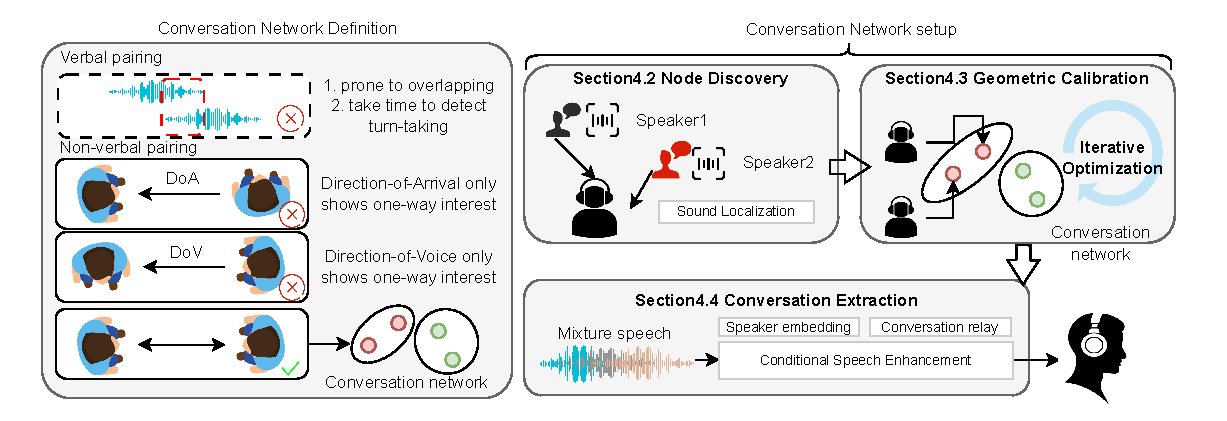
\includegraphics[width=1\linewidth]{chapters/cohear/figs/overview.pdf}
    \vspace{-1em}
    \caption{Overview of the CoHear system. We conduct node discovery for each user and carry out geometric calibration collaboratively. Finally, we perform target conversation extraction based on clues related to the members of the conversation.}
    \label{fig:system overview}
    \vspace{-1em}
\end{figure}

CoHear is a novel network system specifically designed to establish connections based on conversational features, as illustrated in Fig. \ref{fig:system overview}. To achieve this, we define a "conversation network" as the foundation of the system, where individuals participating in the same conversation will experience conversation enhancement.
To construct such a network, the first step is to define its basic components: pairings and which participants are considered part of the same conversation. The details of this definition will be discussed in the next subsection.
Given the definition of the conversation network, the next step is to implement it in the real world using earphones, as shown on the right side of Fig. \ref{fig:system overview}. CoHear employs a two-stage process for conversation modeling. In the first stage, we set up the conversation through acoustic sensing and optimization, and in the second stage, we perform enhancement powered by the network.

The implementation consists of three core components:
First, the \textbf{node discovery} module acts as the front end of our system, where nearby nodes (i.e., speakers) are identified using deep learning-based sound source localization. We extract both the locations and embeddings of each speaker to serve as input for the next stage. Note that this process applies to all speakers wearing earphones; further details are provided in Sec. \ref{sec:acoustic}.
Second, \textbf{geometric calibration} is performed in a centralized manner by aggregating the outputs of the node discovery module from each speaker, as discussed in Sec. \ref{sec:geometric}. Although each node can only observe others within its local coordinate system, we iteratively optimize a shared global geometry. The more observations we obtain from the speakers, the more stable the optimization becomes. After completing the initial optimization with a cold start, we can track the speakers in real time.
Once the conversation network is established, the final component, \textbf{conversation enhancement}, performs conversation-level speech enhancement based on the identified participants (described in Sec. \ref{sec:conversation}). Specifically, both the speaker embedding (time-invariant) and the relay signal (time-variant) are used as cues for the conditional speech enhancement model. We introduce an audio control module to balance the contributions of these two approaches.

\paragraph{Conversational network}
To define our conversation network, the first step is answering the question: How can we technically model the conversation?'' Specifically, we break down a conversation into individual interactions performed by each participant, such as when user A speaks to user B. We observe that such a definition is similar to the concept of computer networking, where a sender sends pairing messages to find a receiver.
Accordingly, we construct a conversation network comprising all participants that can be successfully paired with the same conversation.
It is important to note that existing platforms, such as Livekit \cite{livekit}, provide real-time audio-visual sharing via WebRTC \cite{blum2021webrtc} Selective Forwarding Units (SFUs). In contrast, CoHear builds upon these platforms and extends their capabilities with advanced conversation modeling.

To enable the pairing of networks, we consider two features as discussed in Sec. \ref{sec:related}: verbal and non-verbal. Since the verbal feature (turn-taking) needs to wait for enough time before being effective, we consider the non-verbal feature as the main factor to determine the conversation.
We consider that a person's head orientation is a key indicator of their willingness to engage in conversation, both to speak and to listen. We define a conversation as requiring a bidirectional interest: individuals in the same conversational group must have an interest in at least one other person within the group. This mutual interest is depicted in the bottom left of Fig. \ref{fig:system overview}. As this pairing relies solely on non-verbal cues, we refer to it as the non-verbal pairing of a conversation network.
If we aim to implement this pairing using audio, sound source localization is a natural consideration. However, while sound source localization can estimate a person's relative position, it is insufficient for identifying conversational groups. This is because the DoA of sound can only determine a unidirectional interest (i.e., who is being listened to). Similarly, Direction-of-Voice also only indicates the other way of interest, so that both DoA and DoV are not the indicators for conversation.
Formally, combining both DoA and DoV allows us to infer the desired 6 Degrees of Freedom (6DoF) locations of participants. This necessity motivates us to move beyond the limitations of existing sound source localization methods.

Verbal features, such as turn-taking, serve as direct indicators of conversational engagement, as illustrated in the upper-left section of Fig. \ref{fig:system overview}. However, a significant drawback is their reliance on observing a sufficient duration of speech to be effective (i.e., one must wait for a turn-taking event to occur). Furthermore, overlapping audio is prone to interference from other speakers, which reduces reliability.
Consequently, the conversation network in our current implementation is primarily constructed using non-verbal pairing. Although these non-verbal features are also extracted from the audio signal—the same source as the verbal features—they are processed in a fundamentally different way. This alternative processing method ensures that the two aforementioned disadvantages do not apply to our design.


 


\begin{figure}[h]
    \centering
    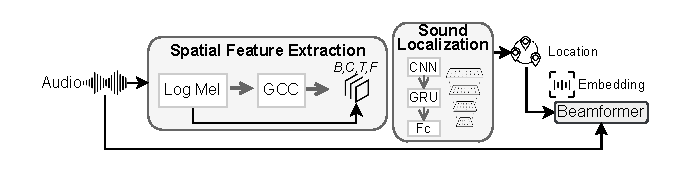
\includegraphics[width=0.7\linewidth]{chapters/cohear/figs/acoustic.pdf}
    \vspace{-1em}
    \caption{The node discovery for conversation setup: where we detect the sound source in the first stage and find the corresponding speaker embedding in the second stage.}
    \label{fig:acoustic}
    \vspace{-1em}
\end{figure}

\subsection{Node Discovery for Conversation Setup}
\label{sec:acoustic}
Conversation can be depicted through the interaction between speakers; the speaker presents the interest according to the direction of the voice (also the direction of the head). In CoHear, each user is considered as one node, where we reformulate speaker localization as a dynamic node discovery problem in a mobile acoustic network, as shown in Fig. \ref{fig:acoustic}. Specifically, it is necessary to access both the location and identity of the nearby nodes. We represent the location in local coordinates (the receiver as the root) and the identity as the voiceprint, which is an embedding that represents the voice of the speaker.

While joint estimation of these properties (similar to sound event localization and detection) is theoretically possible, prior work shows such approaches suffer from computational complexity and poor scalability \cite{wang2022nerc}. Instead, we adopt a decoupled two-stage discovery process that separately handles node localization and identity extraction and then fuses the results for network coordination.

\paragraph{Stage one: sound localization}
As for the sound localization, we extract the cross-channel features as Sec. \ref{sec:background} and utilize a convolutional recurrent neural network (CRNN) to process them, which consists of multiple convolutional layers, a GRU layer, and the final linear layer to predict the output. 
Specifically, we convert the multi-channel audio recording ($M \times T$) into multiple pairs of recordings ($N \times 2 \times T$), where $N$ refers to all the possible combinations. Then, we apply a log-mel spectrogram transformation for each channel and calculate GCC between every pair of channels. Lastly, we concatenate every pair of channels with the original log-Mel spectrograms as the final representations. For example, the feature has a shape of $(2+1) \times T \times F$ for two-channel audio recordings, which can be considered as the input to the neural network. As for the output format, we represent the sound source location in a cartesian coordinate system ($x, y, z$) with a normalized range of one meter radius ($x^2+y^2+z^2 = 1$), where the output dimension of the last linear layer is 3 with a tanh activation. When there is no sound source, the expected $x,y,z$ are set to zero. During inference, we only consider $x^2+y^2+z^2 > 0.5$ as a valid sound source.
Considering the output frame length is 0.1 seconds, we need to set the downsample ratio of the neural network to match it. Given the hop length of the spectrogram is 20ms, the time-dimension downsampling is set to 5. Consequently, the output format is $3 \times T/5$.

The above design only fits in one-source localization; we incorporate the multi-track \cite{cao2021improved} format for multi-source sound localization. Since we are only interested in the location rather than the sound class, the multi-ACCDOA \cite{shimada2022multi} format is unnecessary.
Considering the max number of sources is $n_{max}$, the output of the model is adjusted to $3*n_{max} \times T/5$ instead. Similar to sound separation, multi-source sound localization also needs permutation-invariant training as follows:
\(loss = \min_{\pi \in \Pi} (MSE(pred_\pi, gt))
\), where $\Pi$ refers to all the possible permutations of the sound sources, the above loss intends to find the optimal permutation (the least loss) and then perform back-propagation. 


\paragraph{Stage two: identity extraction}
After localizing all the sound sources, the next step is to associate the sound location with the identities. Although the speaker identities are accessible with the help of existing tools like Pyannotate \cite{bredin2023pyannote}, which supports overlapping speech and multiple speakers. 
However, the association between locations and identities can be difficult since they are two independent attributes. Specifically, the location of each person can be permuted randomly without impacting the results.

To associate them effectively, we can perform beamforming for each detected sound source and check which speaker's sound is amplified, which brings two subsequent problems: 1) how to perform beamforming with a limited microphone array, and 2) how to determine the identity of the beamformed speech. Although there are existing solutions for them respectively, directly combining them can lead to degradation since they are not co-optimized. 
For example, the output from beamforming can still contain noise, so that speaker identity extraction may not handle it well.

We propose a joint model to solve both the beamforming and embedding extraction at the same time. Specifically, we keep the beamformer (e.g., delay-and-sum beamformer) the same and reshape the output from \(B \times C \times T \times F\) to \(B \times T \times (F \times C)\) and use a linear projector with layer normalization to predict the d-vector. In addition, the final d-vector is the average over time. Since the output is not audio, we can not use the common loss function for neural beamformer (i.e., scale-invariant signal-noise ratio), but the cosine similarity loss as follows:
\(\text{L}(\mathbf{A}, \mathbf{B}) = 1- \frac{\mathbf{A} \cdot \mathbf{B}}{\|\mathbf{A}\| \|\mathbf{B}\|}\),
where \textit{A} is an estimated d-vector, and \textit{B} refers to the d-vector from clean speech with the speaker verification model.

In summary, the discovered node can be classified into three groups: self-voice, interested voice, and other voices. Note that the self-voice and interested voices come from a similar direction (i.e., the front of the user) with different distances, so it is hard to differentiate them with direction information only. Instead, we assume that the self-identity is given as prior knowledge, which is practical through offline or online enrollment. As a result, the self-voice can be identified by the similarity with the stored speaker embedding, so that we will not discover it as a new node.

\begin{figure}[h]
    \centering
    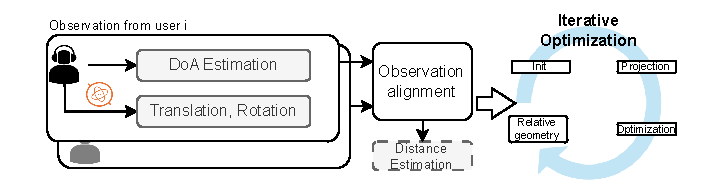
\includegraphics[width=0.7\linewidth]{chapters/cohear/figs/calibration.pdf}
    \vspace{-1em}
    \caption{Network geometric calibration uses the observed distance and direction of arrival, along with user motion, to estimate the locations of all users in the network via iterative optimization.}
    \label{fig:geometric_calibration}
    \vspace{-1em}
\end{figure}

\subsection{Network Geometric Calibration}
\label{sec:geometric}
As outlined in our system overview (Sec. \ref{sec:overview}), our ultimate goal is to estimate the positions of all users (nodes) in a conversation network. The previous node discovery step identifies nearby speakers, providing important positional observations. However, these outputs only indicate where people are speaking, not the structure of the conversation network itself. To achieve this, we propose aggregating observations from multiple participants to estimate the network's underlying geometry.
This task can be formulated as a multi-sensor localization problem, known as geometric calibration. Given that we use acoustic signals for localization, our approach falls within the category of WASN, as discussed in Section \ref{sec:background}.

This section details our geometric calibration pipeline. First, we describe how we obtain the necessary inputs: observation sharing and distance estimation, which provide DoA and distance measurements, respectively. Next, we introduce the concept of a Mobile WASN, distinguishing it from conventional Wireless Acoustic Sensor Networks. We then present our improved geometric calibration algorithm, which estimates the final positions of all nodes. Finally, we address two critical implementation factors: 1) reducing the warm-up time through dynamic calibration, and 2) enabling the system to operate with only a single device.

\paragraph{Observation alignment}
\label{sec:sharing}
The principle of geometric calibration is that one source can be observed by multiple nodes, where the relative position is related to the nodes' positions. Thus, it is important to align the source across nodes.
It is a trivial task when there is only one sound source, but it becomes complicated with 1) overlapping sound, 2) the sound isn't observed by some nodes. Since we have already extracted the corresponding speaker embedding for each source, we can assign the same identity to the sources with similar embeddings.
Specifically, for the speakers observed by one user (including itself), we pair all of them with the observations from other users and only keep the ones that have high similarity. The similarity is calculated by the cosine similarity of two embeddings.
A group of sources with more than 0.8 similarity is considered the same source. We don't make the assumption that one source can be observed by all users.
In practice, every device uploads its observed embeddings from Sec. \ref{sec:acoustic} to a central server and performs the above matching. Only the source that is observed by at least two nodes are considered as valid ones in the following.

\paragraph{Distance estimation}
\label{sec:distance}
According to the output of Sec. \ref{sec:acoustic}, we can only obtain the direction of arrival, while the distance to the sound source is skipped.
However, the distance information is important in geometric calibration since the optimization can be under-determined without it. Ideally, audio recordings already embed distance information in a reverberant environment, as illustrated in the following:
\[
y(t) = h(t) * x(t) + v(t) = h_{e}(t) * x(t) + h_{l}(t) * x(t) + v(t)
\], where \( v(t) \) corresponds to white sensor noise and \( h(t) \) represents the room impulse response, the symbol \( * \) denotes convolution. However, the performance highly relies on a known environment, so the scalability is not satisfying \cite{krause2021joint, gburrek2021geometry}.

Instead, we propose estimating distance by comparing the sound pressure levels at the transmitter and receiver. In an ideal scenario, the audio attenuation corresponds to the propagation path loss, which is related to distance. To ensure a clean input signal and mitigate the effects of multi-path propagation or overlapping sound sources, we selectively use audio segments containing only a single active source and compute the average sound level from these segments.
Despite this design, distance estimation errors may still be significant. Therefore, we do not use the estimated distance as a final output. Instead, we utilize it as an input for subsequent geometric calibration, alongside other data.



\paragraph{Mobile WASN}
According to Sec. \ref{sec:background}, our network can be considered as mobile WASN, an extension of WASN where the acoustic node can move freely. Similarly, localization of sensor nodes can be achieved by geometric calibration, given sufficient observed sound sources. Compared to the conventional notation, mobile WASN has different assumptions as follows.

\begin{enumerate}
    \item First, the assumption that only one sound source is present during a measurement is unrealistic due to the possibility of overlapping speech and other background sounds. Specifically, if we denote the maximum number of simultaneous speech sources as \(M\), we can estimate a total of \(M \times K \times L\) instances, which is also compatible with fewer than \(M\) number of sources by adding a blank estimate.
    \item Second, while all the estimates are considered valid in the previous context, the arbitrary movement of users can create a much greater distance between two sensor nodes, which means that some sound sources may not be observed by all sensor nodes.
    \item Third, the acoustic source \(S_{k}\) is defined as the \(k^{th}\) observed source during a specific time period. In this context, \(k\) (where \(k = 1, 2, \ldots, K\)) can also serve as a time identifier. The notation is important because we can align the sound source with the location of the sensor nodes, which are also time-dependent and can be represented as \(n_{k,l}\). Since the sensor nodes can move freely, we use \(T_{k,l}\) and \(R_{k,l}\) to indicate the translation and rotation between \(n_{k,l}\) and \(n_{0,l}\) for the \(l^{th}\) node.
    \item Lastly, it is expected that \(n_{k,l}\) will match at least one of the \(S_{k}\) since the sensor node is one of the sound sources. Note that it is not valid conversely since there are sound sources that come from people without earphones. 
\end{enumerate}


\paragraph{Geometric calibration}
We perform mobile geometric calibration with the networked earphones, which share a similar principle as other geometric calibrations that minimize a cost that is defined to evaluate how well these converted observations align with the assumed geometry. Among the various algorithms, data set matching is an efficient algorithm for geometric calibration. Our algorithm is based on that of \cite{gburrek2021geometry}; the details of it are out of the scope of this paper.. 

Different from the original algorithm, we have a rotation matrix \(R_{k,l}\) and a translation vector \(n_{k,l}\) that are dependent on both the source and the node. As a result, we rewrite the relative locations in the global coordinates:
\[
G_{k,l} = R_{k,l} d_{k,l} [cos(\theta_{k,l}), sin(\theta_{k,l})] + n_{k,l}
\]
Multiple nodes observe each source at the same time; if all the estimates are perfectly right, all \( S_{k,l}\) would map to a unique position \( G_{k,l} \). Hence, the geometry can be inferred by minimizing the deviation of the projected source positions by the cost function below:
\[
\arg\min \sum_{l=1}^{L} \sum_{k=1}^{K} \left\| G_{k,l} - S_{k,l} \right\|_2^2
\]
, where \( \| \cdot \|_2 \) denoting the Euclidean norm. There exists no closed-form solution for the above nonlinear optimization problem, so it has to be solved using an iterative optimization algorithm.

Compared to our setting, previous methods estimate 
\(R_{l}\) and translation \(n_{l}\) for L sensor nodes, while ours estimate \(K \times L\) nodes equivalently. The naive approach is performing geometric calibration for each source, downgrading to K times one source geometric calibration, and merging the results afterward.
According to the analysis in \cite{gburrek2021geometry}, the performance of geometric calibration depends on the number of sources. Consequently, the one-source geometric calibration will give unreliable results and harm the final performance.

Instead, we can further compose the translation into initial and movement: 
\(R_{k,l} = \overline{R}_{k,l}R_{0,l}\) and \(n_{k,l} = \overline{n}_{k,l} + n_{0,l}\), where \(\overline{R}_{k,l}\) refers the rotation from the first source to the k source for sensor l and \(\overline{n}_{k,l}\) refers the corresponding translation. We can see that if the \(\overline{R}_{k,l}\) is an identity matrix and \(\overline{n}_{k,l}\) is zero, the problem downgrades to the same as \cite{gburrek2021geometry}. As a result, we rewrite the above equation:
\[
G_{k,l} = R_{0,l} d_{k,l} \overline{R}_{k,l} [cos(\theta_{k,l}), sin(\theta_{k,l})] + \overline{n}_{k,l} +  n_{0,l}
\]
Fortunately, we can estimate \(\overline{R}_{k,l}\) and \(\overline{n}_{k,l}\) by a motion sensor on the node, which means our estimation targets become \(R_{0,l}\) and \(n_{0,l}\) so that the problem becomes estimating one locations instead of track. In other words, we can apply the data set match algorithm in the appendix.

In addition, the above processing can be generalized to multiple sources. Suppose \(M\) is the maximum number of simultaneous sources, the \(\overline{K}\) refers to the real number of sources within K times (\(K\leq\overline{K}\leq M \times K\)). We can set the \(R\) and \(n\) accordingly to fit in the original setting.

\paragraph{Dynamic calibration}
Based on our design, we conduct geometric calibration for every \(\overline{K}\) observation, which is not ideal for real-time inference. As a solution, we implement a sliding-window approach that allows us to repeat geometric calibration each time we receive new observations. Given that the runtime latency for this process is minimal, we plan to address the optimization in future work.

Meanwhile, selecting an optimal \(\overline{K}\) becomes critical, as it seems to be related to the latency and performance. Although the correlation between latency is obvious, the correlation with performance can be complicated. Specifically, the motion estimation (\(\overline{R}_{k,l}\) and \(\overline{n}_{k,l}\)) by IMU is also poisoned by accumulated errors with increasing \(\overline{K}\), which means the calibration may not be accurate with a large \(\overline{K}\). A small sliding window can be a direct solution to mitigate the degradation caused by noisy estimates. However, since the optimization needs sufficient observations to converge, the small window can conversely degrade the usability. Instead, we propose a weight decay algorithm where the calibration results focus more on the nearest observations. Specifically, we set the weight as \(  1/ (T-t)\), where \(T-t\) refers to the difference between the current time and the time of observations.

\paragraph{Single-device solution}
While collaborative calibration is the optimal approach, we propose a single-device method for scenarios where networking is impractical or latency is critical. In the evaluation, the above design will be considered as a special case when there is one earphone.
In geometric calibration, the output for each user is their position (\(P=(x_i, y_i)\))and orientation (\(O=\theta\)) within a shared coordinate system. However, in a single-user scenario, the shared coordinate system is defined relative to the user themself. In this case, the source's position and orientation relative to the user can be described by three key variables: the Direction of Arrival, the distance to the source, and the source's own orientation.

Assuming the sound source localization method from Section \ref{sec:acoustic} provides a reliable DOA, we note that the distance and source orientation variables are still missing. To address this, we modify our model to estimate these two additional variables.
Our neural network already outputs a 3-dimensional vector. We remove the unit vector constraint (\(x^2+y^2+z^2=1\)) to allow the model to represent sources at any distance. Furthermore, we add four additional output nodes to classify the sound source's orientation into one of four categories: front, left, right, or back. We use classification instead of regression for the orientation, as this challenging problem benefits from the increased stability that a classification approach provides.

\begin{figure}[h]
    \centering
    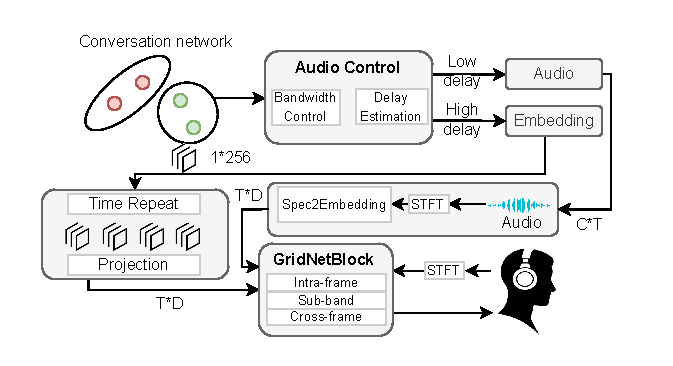
\includegraphics[width=0.7\linewidth]{chapters/cohear/figs/conversation_extraction.pdf}
    \vspace{-1em}
    \caption{Conversation extraction by target feature, which can be classified into time-invariant (speaker embedding) and time-variant. The adaptive audio control can balance the quality and bandwidth before sending to the neural network model.}
    \label{fig:voice_share}
    \vspace{-1em}
\end{figure}



\subsection{Conversation Extraction}
\label{sec:conversation}


\paragraph{Problem formulation}
For each group of nodes participating in the same conversation, the locations, identities (represented by speaker embeddings), and the audio recordings are shared among all members. We utilize this information to adjust the user's hearing (extract conversation) as demonstrated in Fig. \ref{fig:voice_share}.

Our design goal is to extract a target conversation from a speech mixture under specific conditions. While raw audio provides more fine-grained information than speaker embeddings, it consumes significantly more bandwidth. A naive solution, assuming we have access to a relatively clean audio relay, would be to transmit this audio directly like a video conference. However, this assumption is impractical for two reasons. First, even after noise suppression, we cannot guarantee that the transmitted audio perfectly matches the target speech. Second, the transmission process itself introduces delay, packet loss, and compression artifacts, resulting in a degraded version of the original received audio. Therefore, the core problem we address is how to design a conversation extraction model that can effectively utilize this degraded relay audio.

\paragraph{Adaptive audio control}
Ideally, relay audio should be transmitted at the highest possible quality. However, there will always be a bandwidth bound, particularly with multiple concurrent users. This is a common problem in networking, addressed by algorithms like TCP congestion control.
Unlike these well-established solutions, CoHear also considers the acoustic noise level, where a higher noise level indicates the need for a larger bandwidth (to provide more information as compensation). 
To achieve this, we can perform a grid search to maximize the overall conversation quality for all users under a total bandwidth constraint. For each user, we consider the distance as the indicator for conversation quality instead of directly estimating the metric like SNR. Consequently, the search objective is the sum of bandwidth/ distance for all the users within the conversation, where the total bandwidth is constrained. The reason behind our design is the close correlation between pair-to-pair distance and noise level.

Besides the bandwidth, transmission delay is another factor that needs consideration. Specifically, a delayed audio is almost useless even if he audio quality is good since the time-dimension correlation between the time-variant feature and the target speech diminishes, reducing its effectiveness as a reference. 
To address this, we propose estimating the transmission delay and disabling the time-variant feature when the latency exceeds a certain threshold. 
Specifically, we can utilize the GCC technique between the transmitted audio and the noisy speech, identifying the first peak as the delay.
Note that we don't need to estimate the delay frequently since we assume the delay is relatively stable.
In our empirical test, we find that a delay of 50ms is still tolerable for the time-variant feature and set it as the threshold.
Consequently, under poor network conditions, the system gracefully degrades by relying solely on time-invariant features for target speech extraction.
It is also important to note that the switch between time-invariant and time-variant features impacts bandwidth control. When audio transmission is not necessary (i.e., when the time-variant feature is disabled), the bandwidth requirement can be reduced accordingly.


\paragraph{Target conversation extraction}
Given the above analysis, the time-variant feature can be viewed as an extension of the time-invariant feature. Although the former provides richer information, several factors beyond bandwidth—such as latency, noise, and transmission losses (e.g., packet loss, bit errors)—can degrade the quality of these features.
Building on prior work in target speaker extraction \cite{veluri2024look}, we focus on target conversation extraction as an extension of speech enhancement. Existing target speech extraction methods typically rely on either time-invariant features, such as embeddings \cite{chen2024target, veluri2024look} or time-variant data like bone-conducted vibrations \cite{he2023towards}.
Time-invariant features, while compact and stable, can be viewed as ultra-highly compressed audio, potentially losing fine-grained details compared to time-variant data, like bone-conducted vibrations \cite{he2023towards} or relay audio \cite{shen2018mute}. To address this, CoHear is designed to strike a balance between compression and performance, optimizing both efficiency and accuracy.

Considering the time-invariant feature like speaker embedding, the enrollment speech (from the target user) is first converted to the speaker embedding by an encoder. To fit the feature in the model, the speaker embedding is projected to the same feature dimension and repeated to align with the time dimension. Lastly, the speaker embedding in the time-frequency dimension is added to the enhancement network. The pipeline is illustrated as follows:
\[
y = TSE(y_{noisy}, [e_{enrollment}, ....]_{T}), \quad e_{enrollment} = Embedder(y_{enrollment})
\], where the $TSE$ refers to the target speech extraction model (i.e., modified TFGridNet) and $Embedder$ refers to the speaker embedding extractor. We consider that $y_{enrollment}$ comes from the target user whose voice is mixed with noise in $y_{noisy}$.
As for the time-variant feature, which also refers to the target speech as the speaker embedding. We can transform the relay audio into a time-frequency feature using an STFT encoder. Similarly, the feature is added to the enhancement model, and the pipeline is illustrated below:
\[
y = TSE(y_{noisy}, [e_{enrollment}, ....]_{T}, E_{relay}), \quad E_{relay} = Embedder(y_{relay})
\]. To maintain compatibility with time-invariant features, we include both time-invariant features and time-variant features during the training by setting the features to zero when it is absent. Note that the actual form of the time-invariant feature is not the raw audio; we can further improve the efficiency by only transmitting the feature, and we leave it for future work. 
Besides, CoHear is expected to work well with multiple conditions (participants). A naive solution is to apply the speech filter multiple times, which is computation-intensive. Instead, we propose an attention mechanism that combines multiple conditions into the intermediate feature as follows: 
\(
 X = Attention([X_0, X_1, ...])
\)
, where \(X_i\) refers to the \(i^{th}\) conditions.








% \section{Implementation}

\subsection{Implementation and Evaluation Setup}
\begin{figure}
    \centering
    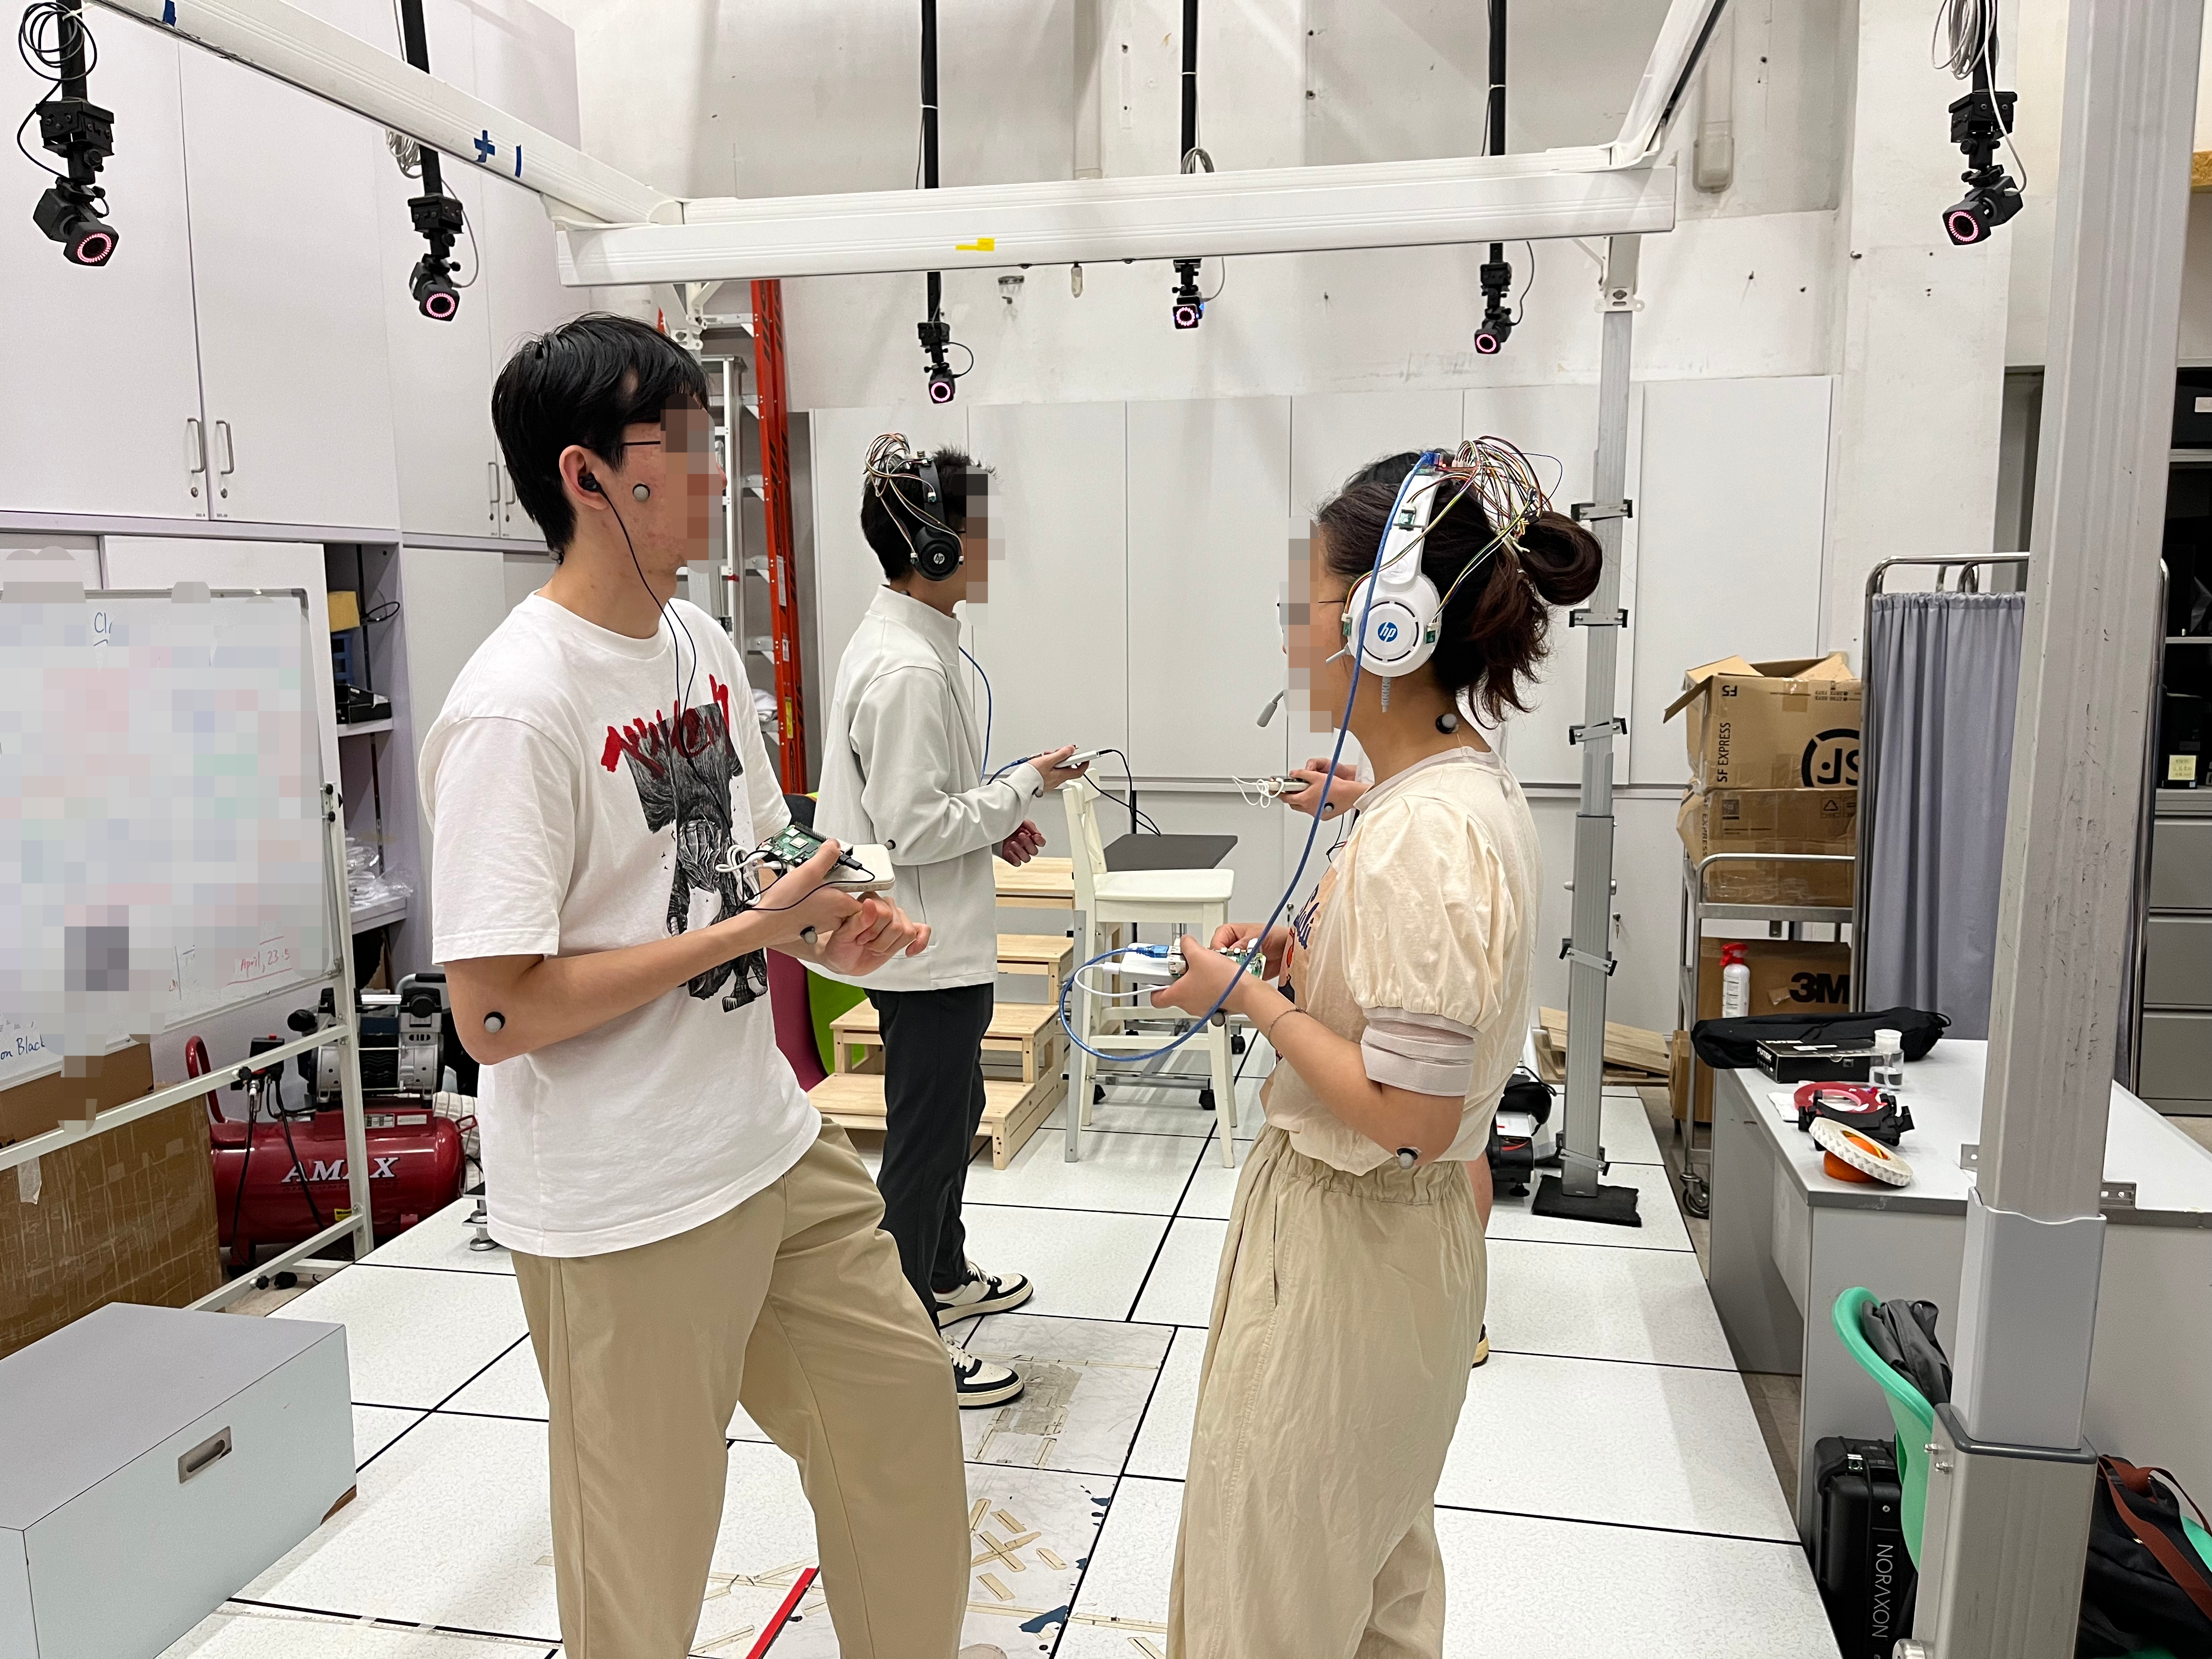
\includegraphics[width=0.5 \linewidth]{chapters/cohear/figs/experiment.png}
    \caption{Experiment setup of the motion capture room.}
    \label{fig:mocap}
    \vspace{-1em}
\end{figure}


\paragraph{Testbed Setup}
\label{sec:cohear_hardware}
We implement CoHear in various form factors, including binaural earphones and headphones with up to an 8-channel microphone array (placement is illustrated in Fig. \ref{fig:mic_loc}). The two earphones are shown in Fig. \ref{fig:hardware}. We use a Raspberry Pi 5 to collect audio and attach one IMU (BMI-160) to the headphones to track head motion, transmitted via I2C. For experimental validation, we connect each device via SSH under the same WiFi network, streaming all data to a desktop for analysis. The system output is designed to be played back through the headphone speakers, maintaining compatibility with existing ANC functionality. 

While our hardware supports sampling rates up to 48 kHz for maximum capture capability, the system is designed to operate at lower rates suitable for real-world deployment.
For practical speech applications, CoHear can operate at 8 kHz with audio compression to minimize bandwidth requirements, which is also evaluated in the later section.
Moreover, CoHear supports time-invariant speaker embeddings that require only one-time transmission, significantly reducing data size to 8192 bits in total, which is practical on even constrained networks. We also discuss the networking issue in Sec. \ref{sec:cohear_discuss}.


\begin{figure}[t]
    \centering
    \begin{minipage}{0.48\linewidth}
    \centering
    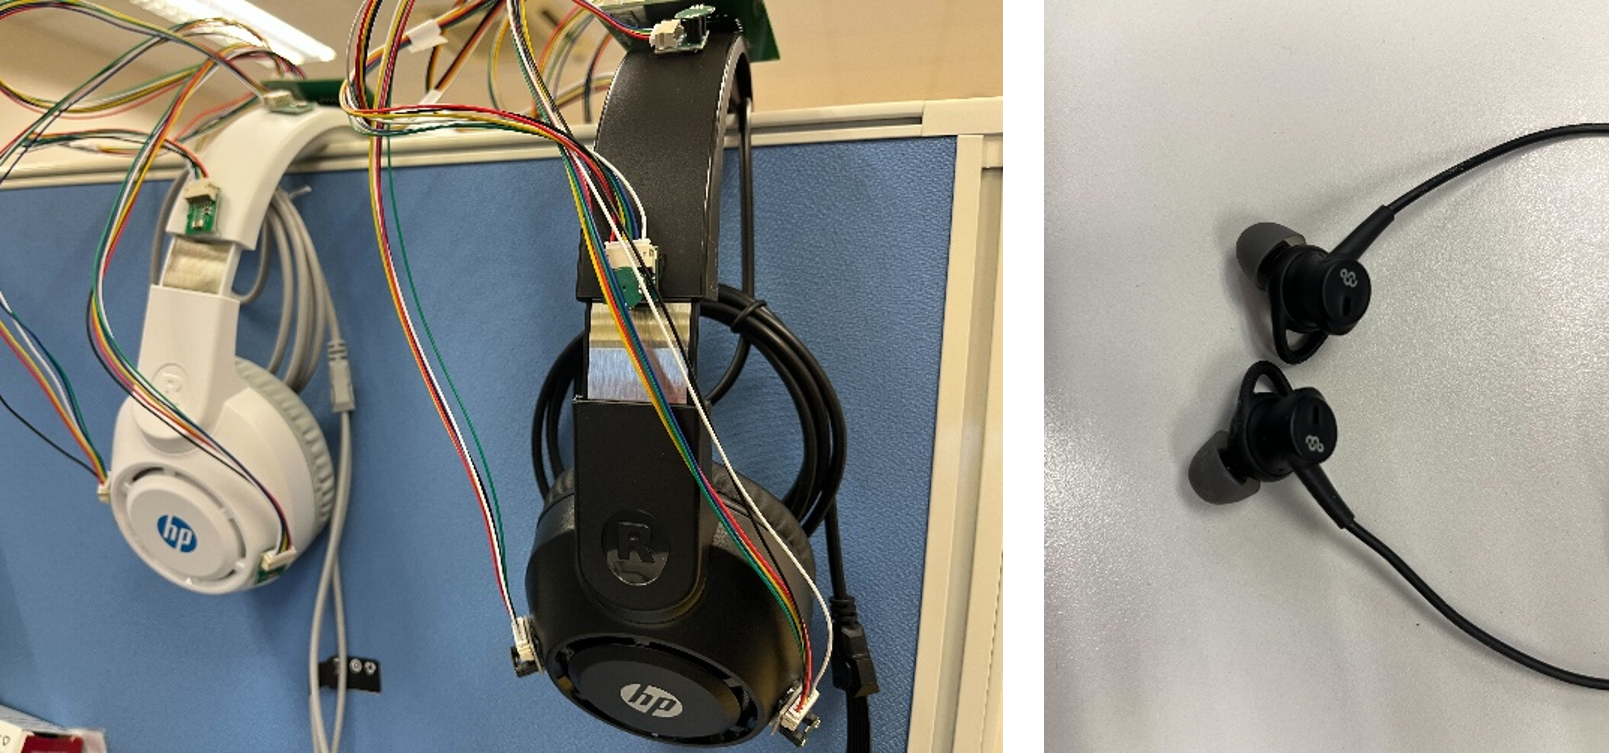
\includegraphics[width=0.8\linewidth]{chapters/cohear/figs/device.png}
    \caption{Hardware used in the experiment.}
    \label{fig:hardware}
    \end{minipage}
    \hfill
     \begin{minipage}{0.48\linewidth}
        \centering
        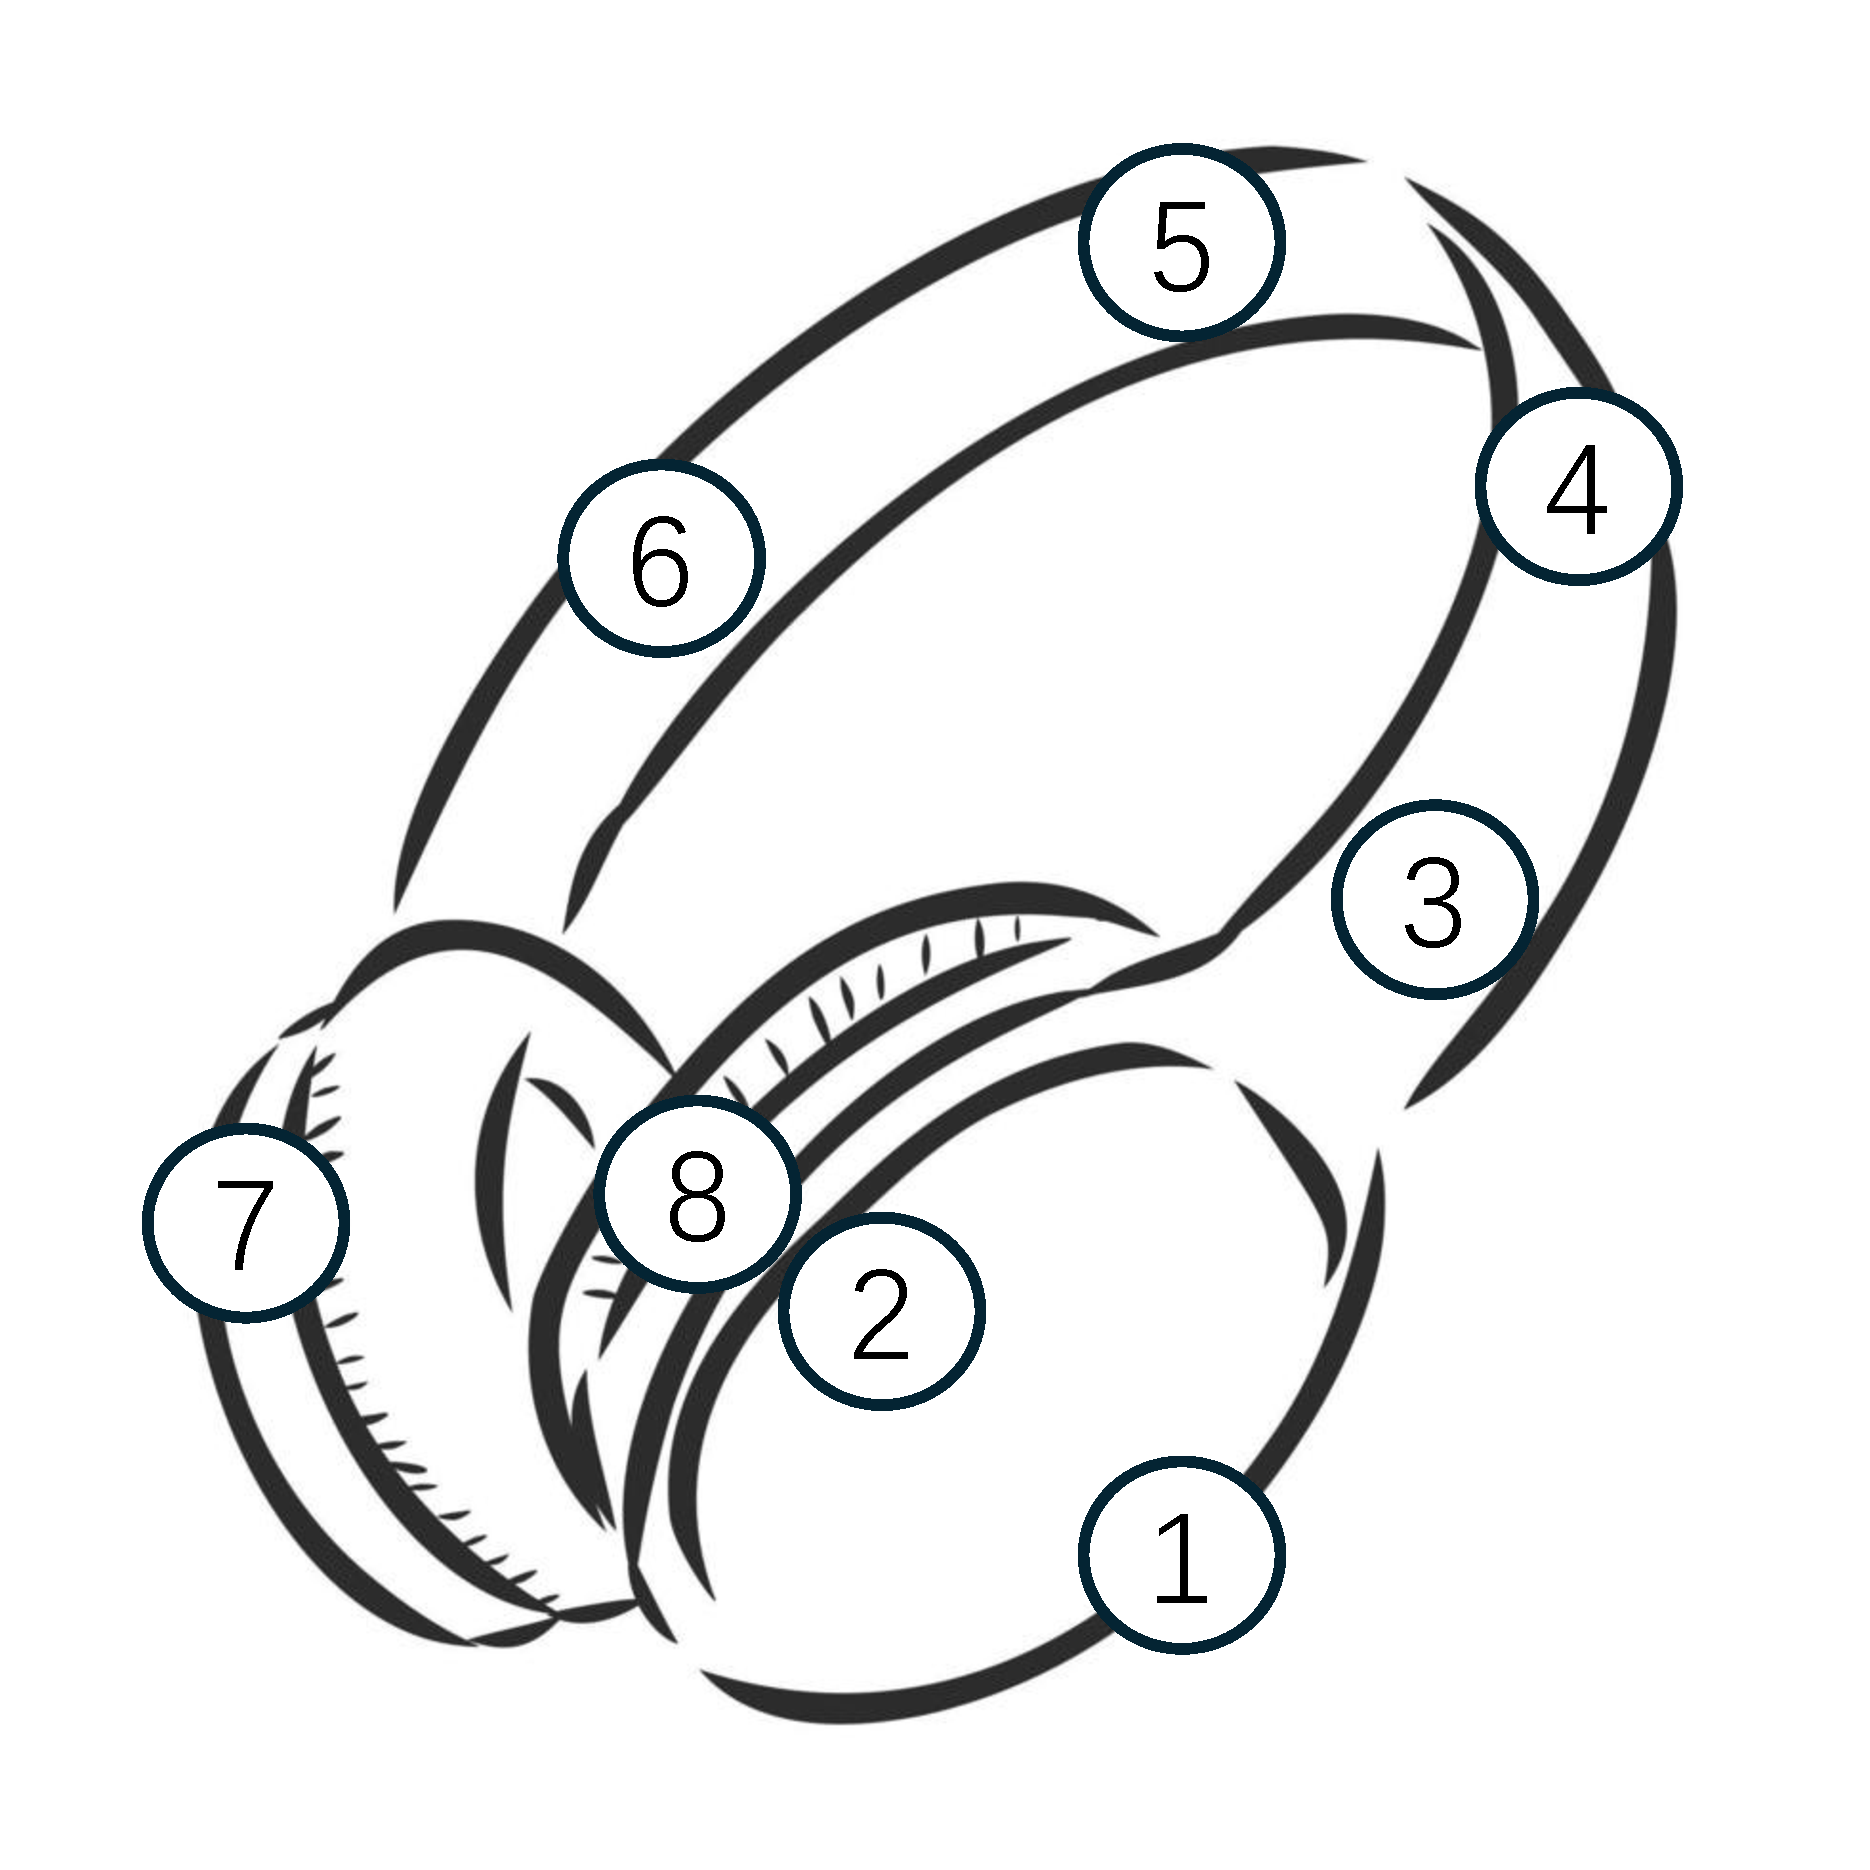
\includegraphics[width=0.4\linewidth]{chapters/cohear/figs/mic_loc.pdf}
    \caption{Microphones location on the headphone.}
    \label{fig:mic_loc}
    \end{minipage}%
    \vspace{-1em}
\end{figure}


\paragraph{Dataset Collection}
We use three data sources to support the design and evaluation of CoHear: a real-world dataset collected in a motion capture room, simulated datasets for large-scale testing and training, and public datasets for comparison.

\vspace{1ex}
\noindent\textit{Real-world Collection:}
We collected 30 minutes of multi-person conversation data in a $10 \times 5$ m motion capture room equipped with a 12-camera VICON system (Fig.~\ref{fig:mocap}). Markers were placed on participants’ heads and upper bodies to track conversational poses. Six volunteers wore our prototype headphones (Section~\ref{sec:cohear_hardware}) and engaged in natural turn-taking conversations. Due to space limitations, each session involved 2–4 participants in different grouping scenarios:
1) two participants in one group,
2) three participants with one excluded, and
3) four participants split into two groups.

\vspace{1ex}
\noindent\textit{Simulation:}
To scale beyond the limits of physical collection, we simulate two datasets: 1) Geometric Calibration: Using Pyroomacoustics~\cite{scheibler2018pyroomacoustics}, we simulate dynamic conversations in larger rooms (up to 20 m wide) with varied reverberation (RT60 from 0.25 to 0.75).
And 2) Conversation Extraction: We augment the real dataset with noisy-clean pairs and degraded relays (e.g., SNR, compression, bit crush, packet loss) to train and evaluate the enhancement model. The SNR of the noisy speech is set to between -10 dB and 10 dB.

\vspace{1ex}
\noindent\textit{Public Datasets:}
We also compare CoHear with existing datasets in Table~\ref{tab:comparison_dataset}. While prior work such as STARSS23~\cite{shimada2024starss23} and 6DoF-SELD~\cite{yasuda20246dof} focuses on sound event localization, and AMI~\cite{kraaij2005ami} and EasyCom~\cite{donley2021easycom} cover conversations, none support collaborative multi-device conversation modeling with 6DoF tracking as CoHear does.

\begin{table}[t]
\caption{Comparison with existing datasets.}
\centering
\begin{tabular}{|c|c|c|c|}
\hline
\textbf{Name} & \textbf{6DoF} & \textbf{Multi-device} & \textbf{Target} \\
\hline
STARSS23~\cite{shimada2024starss23} & No & No & Sound events \\
6DoF-SELD~\cite{yasuda20246dof} & Yes & No & Sound events \\
AMI~\cite{kraaij2005ami} & No & No & Conversation \\
EasyCom~\cite{donley2021easycom} & Yes & No & Conversation \\
\textbf{CoHear} & \textbf{Yes} & \textbf{Yes} & \textbf{Conversation} \\
\hline
\end{tabular}
\label{tab:comparison_dataset}
\end{table}



\paragraph{Evaluation Metrics}
The primary objectives of CoHear are to identify user locations and extract relevant conversations, assessed through distinct metrics.

For geometric calibration, we use two standard metrics: average direction error (in degrees) and location error (in meters). We also incorporate network setup accuracy, which indicates whether the participant can find the correct partner. Specifically, we define \(S_{i,j}\) equals to true if \(|R_{i,j} - O_i| < \frac{\pi}{4}\), where \(R_{i,j}\) is the relative direction from user \(j\) to user \(i\) and \(O_i\) is the orientation of user \(i\). 

As for the conversation enhancement, we will utilize the scale-invariant signal-to-noise ratio (Si-SNR) as a conversation-related metric, noting that the input SNR significantly influences results. Since the average default input SNR is set to 0 dB, allowing the output SNR to reflect improvements over the input.

\paragraph{Baselines Approaches}
Similar to the metrics, we also incorporate different baselines for the geometric calibration and conversation extraction, respectively.
For the former one, we consider \cite{gburrek2021geometry} as the baseline, which is designed for static WASN only. Besides, infrastructure-based acoustic localization \cite{gburrek2021geometry} and acoustic-SLAM \cite{evers2018acoustic} are related to CoHear. Note that when we apply \cite{gburrek2021geometry} as infrastructure-based acoustic localization, we have static nodes but mobile sources (i.e., users); our target becomes estimating the sound sources rather than nodes. We will use the following abbreviations in this paper: DSM refers to baseline \cite{gburrek2021geometry}, iDSM refers to infrastructure-based acoustic localization \cite{gburrek2021geometry}, and aSLAM for acoustic-SLAM \cite{evers2018acoustic}.


As for the conversation extraction, we consider LookOncetoHear \cite{veluri2024look}, target conversation extraction \cite{chen2024target}, and CoS \cite{jenrungrot2020cone} as our baselines. We also replace the relay audio with time-dependent speaker embedding as a baseline.
For LookOncetoHear \cite{veluri2024look}, we assume the enrollment happened in every sentence and takes effect in the next sentence. For the second baseline, we consider self-voice to be the condition. As for the CoS \cite{jenrungrot2020cone}, we assume the interferences span randomly in the nearby space while the target speaker is always in front of the user.
We will use the following abbreviations in this paper: LOTH stands for LookOnceToHear \cite{veluri2024look}, TC refers to \cite{chen2024target}, CoS refers to \cite{jenrungrot2020cone}


\section{Evaluation}

% Evaluation Setup
% \section{Implementation}

\subsection{Implementation and Evaluation Setup}
\begin{figure}
    \centering
    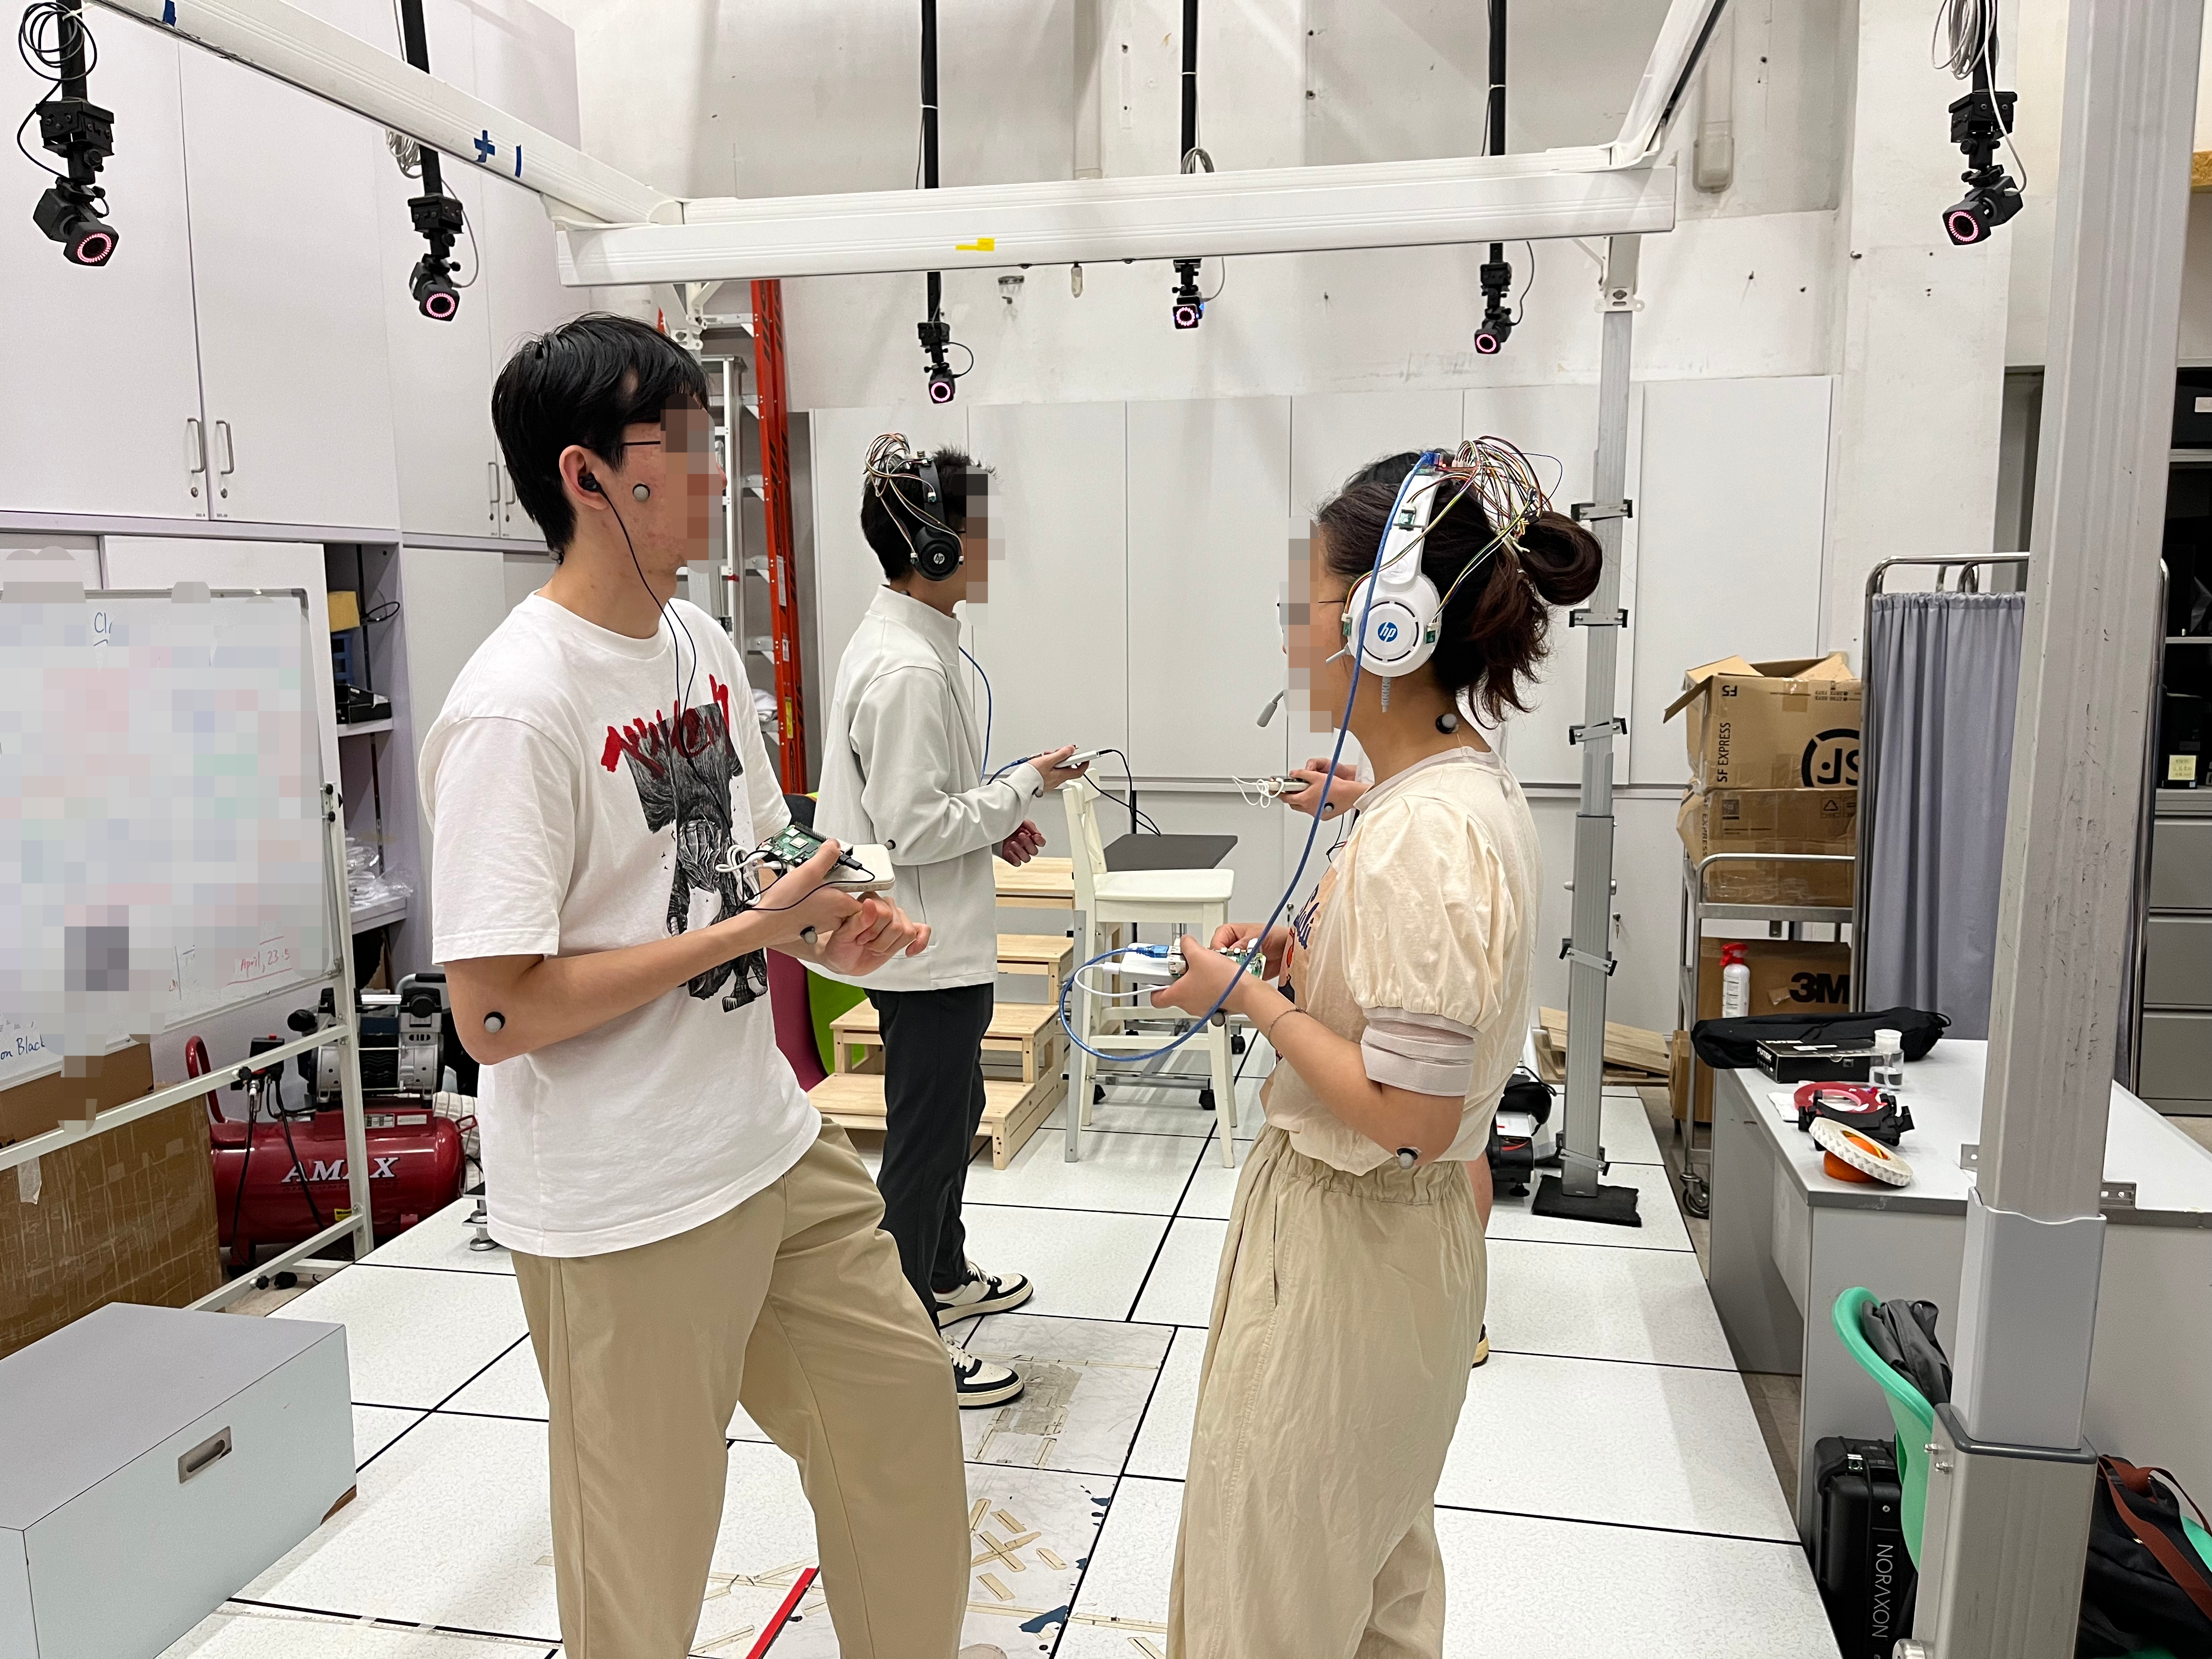
\includegraphics[width=0.5 \linewidth]{chapters/cohear/figs/experiment.png}
    \caption{Experiment setup of the motion capture room.}
    \label{fig:mocap}
    \vspace{-1em}
\end{figure}


\paragraph{Testbed Setup}
\label{sec:cohear_hardware}
We implement CoHear in various form factors, including binaural earphones and headphones with up to an 8-channel microphone array (placement is illustrated in Fig. \ref{fig:mic_loc}). The two earphones are shown in Fig. \ref{fig:hardware}. We use a Raspberry Pi 5 to collect audio and attach one IMU (BMI-160) to the headphones to track head motion, transmitted via I2C. For experimental validation, we connect each device via SSH under the same WiFi network, streaming all data to a desktop for analysis. The system output is designed to be played back through the headphone speakers, maintaining compatibility with existing ANC functionality. 

While our hardware supports sampling rates up to 48 kHz for maximum capture capability, the system is designed to operate at lower rates suitable for real-world deployment.
For practical speech applications, CoHear can operate at 8 kHz with audio compression to minimize bandwidth requirements, which is also evaluated in the later section.
Moreover, CoHear supports time-invariant speaker embeddings that require only one-time transmission, significantly reducing data size to 8192 bits in total, which is practical on even constrained networks. We also discuss the networking issue in Sec. \ref{sec:cohear_discuss}.


\begin{figure}[t]
    \centering
    \begin{minipage}{0.48\linewidth}
    \centering
    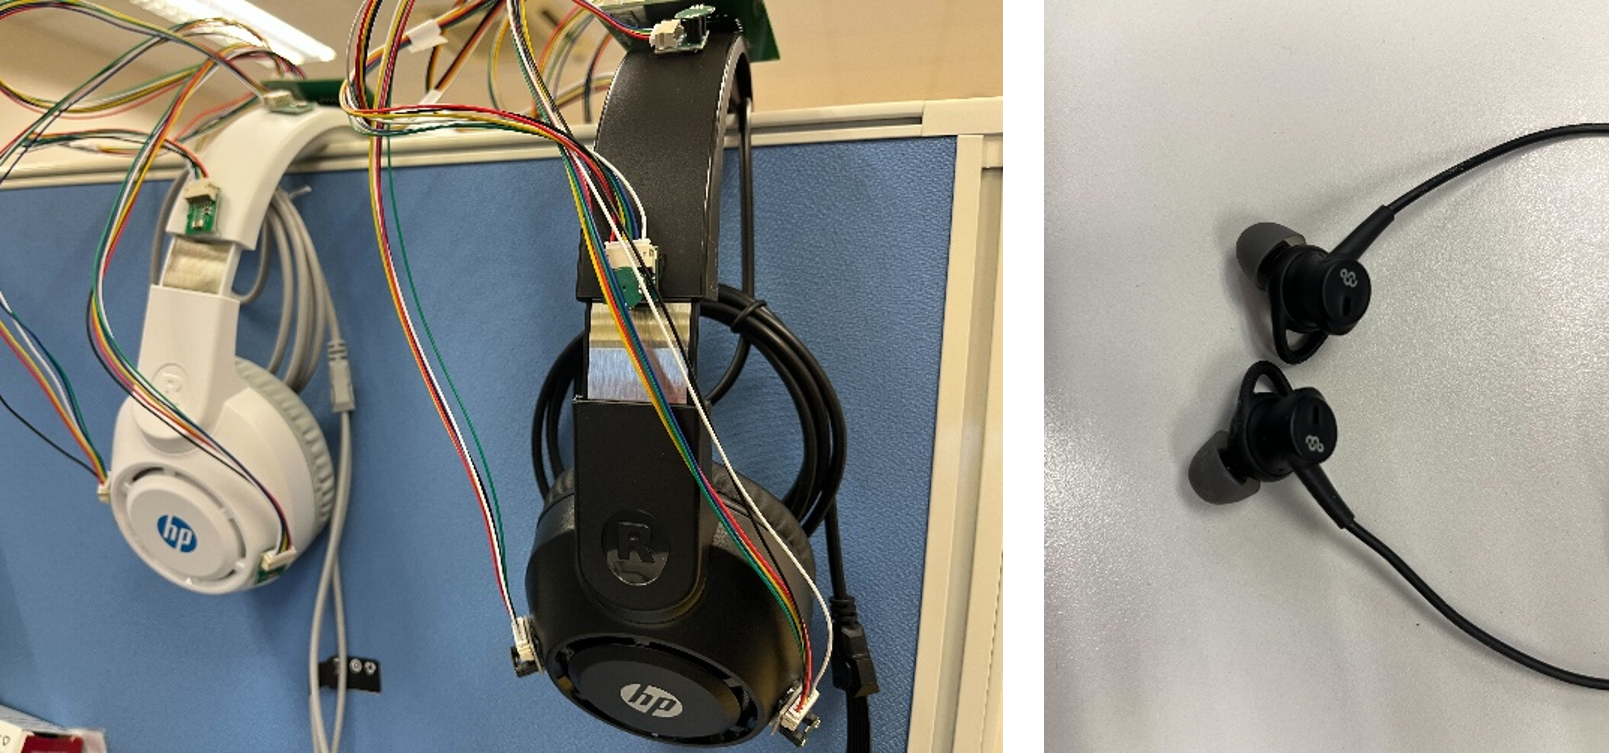
\includegraphics[width=0.8\linewidth]{chapters/cohear/figs/device.png}
    \caption{Hardware used in the experiment.}
    \label{fig:hardware}
    \end{minipage}
    \hfill
     \begin{minipage}{0.48\linewidth}
        \centering
        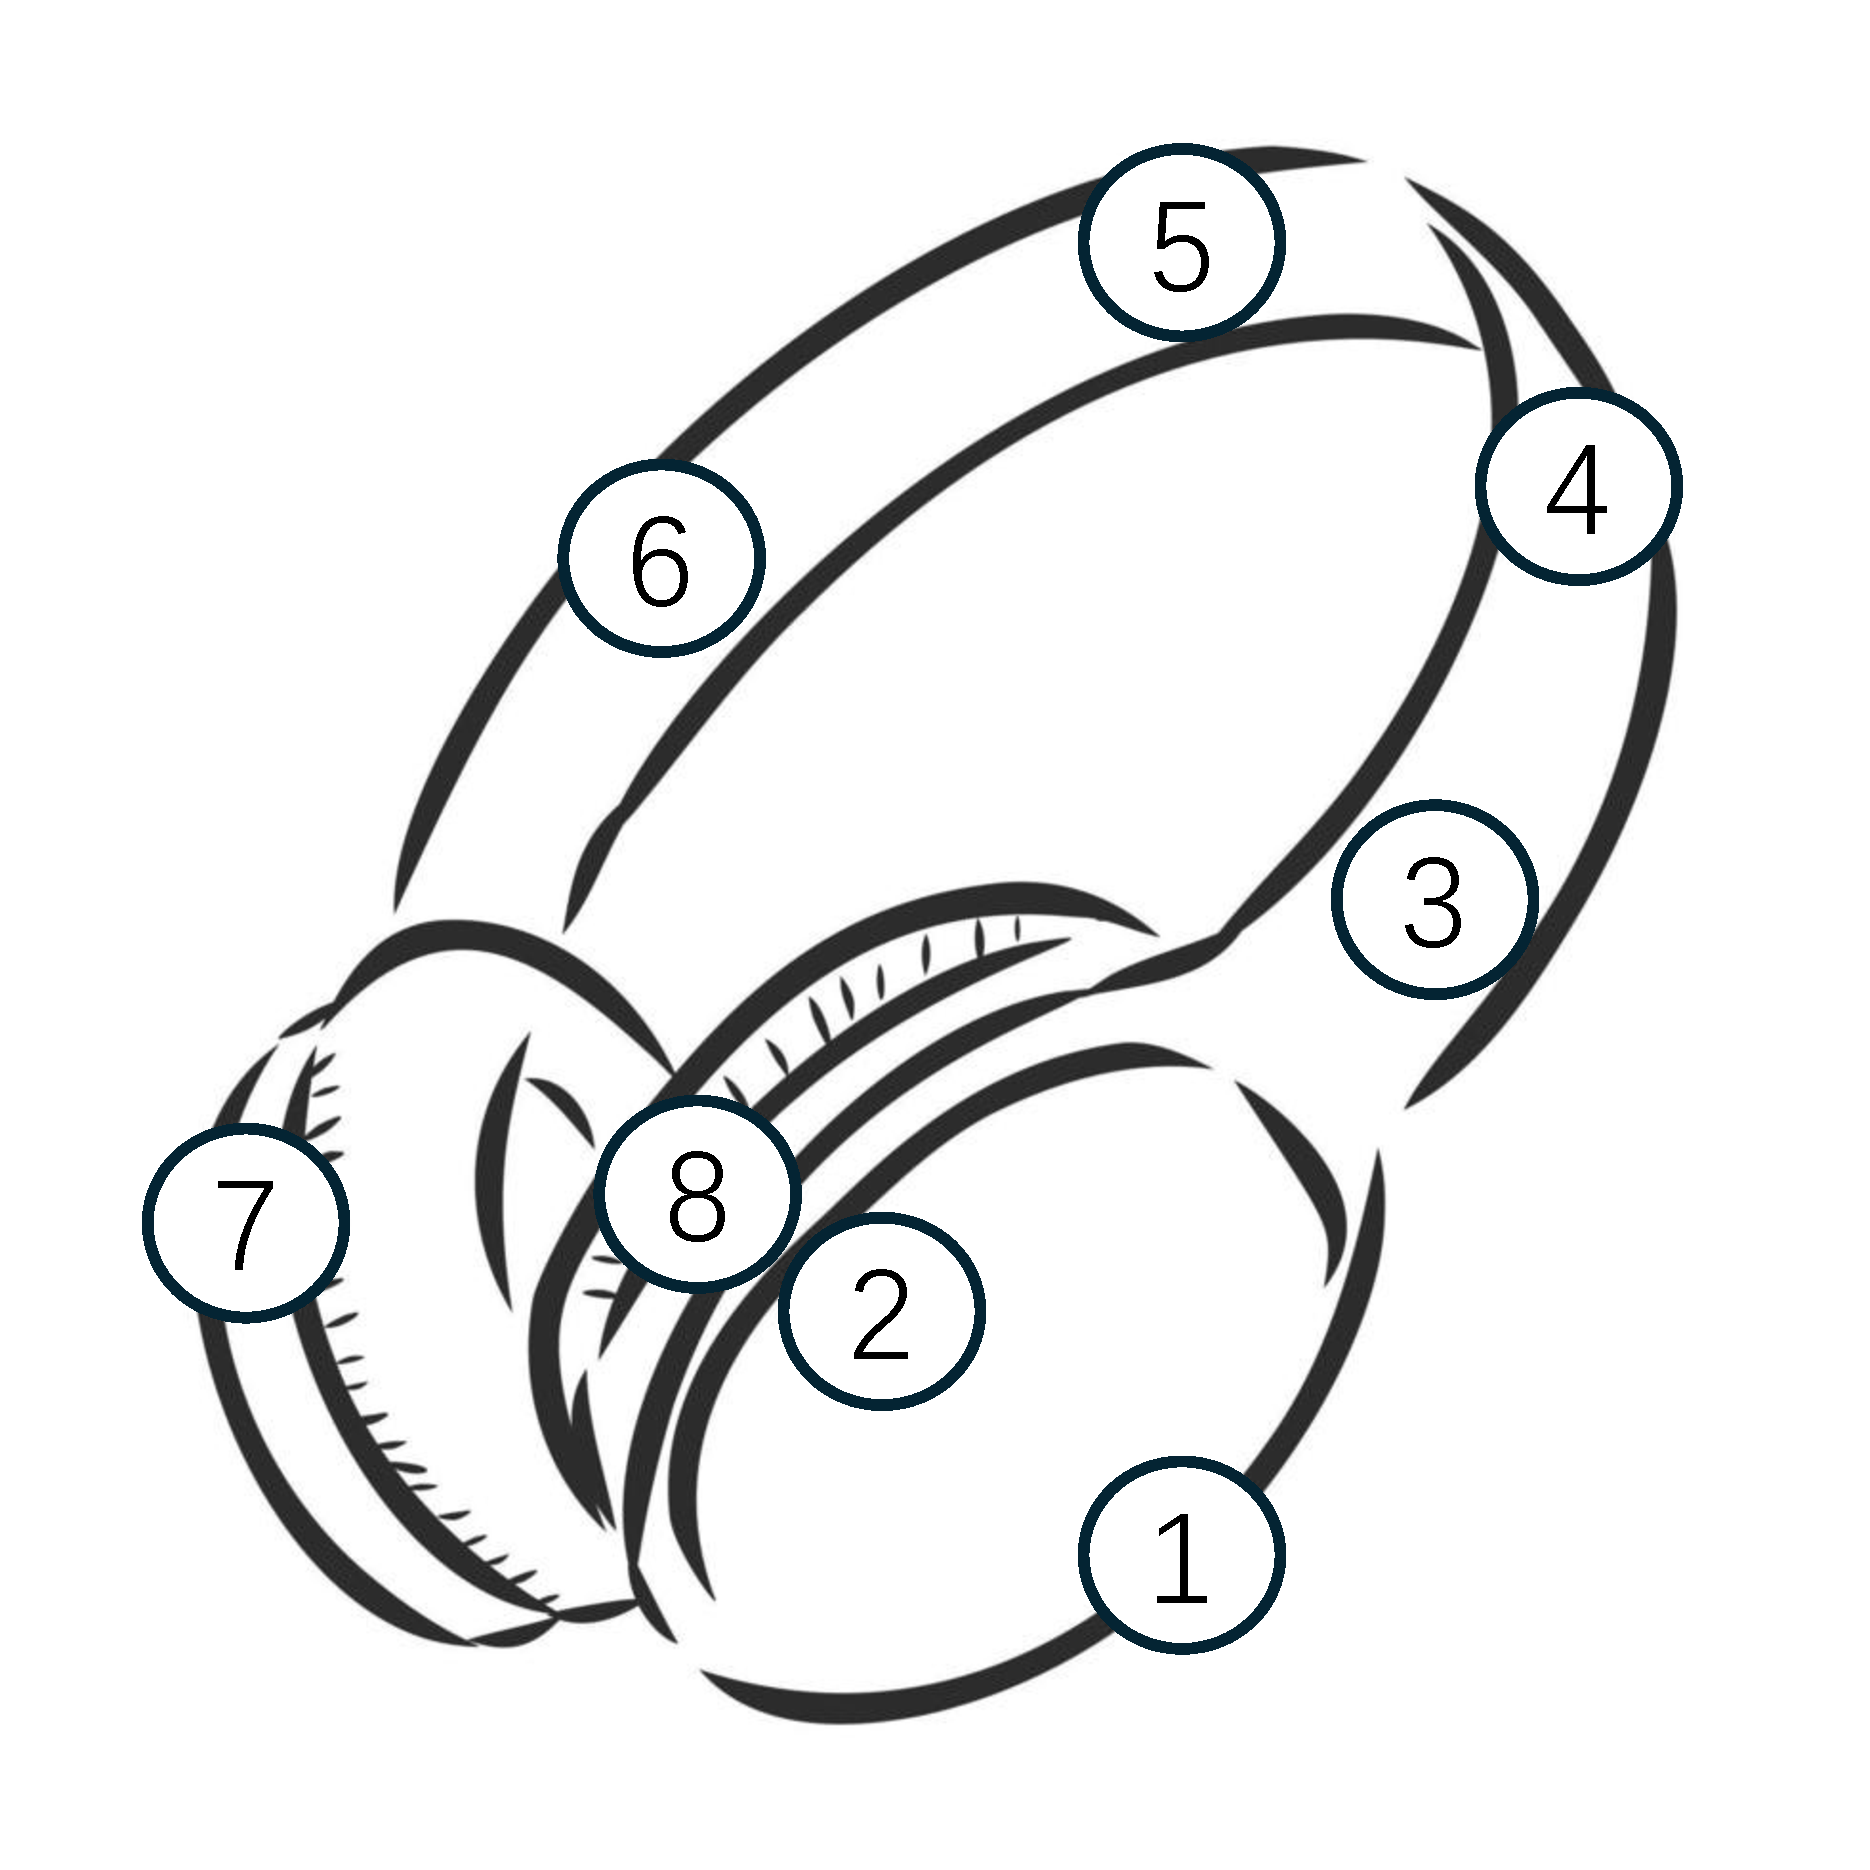
\includegraphics[width=0.4\linewidth]{chapters/cohear/figs/mic_loc.pdf}
    \caption{Microphones location on the headphone.}
    \label{fig:mic_loc}
    \end{minipage}%
    \vspace{-1em}
\end{figure}


\paragraph{Dataset Collection}
We use three data sources to support the design and evaluation of CoHear: a real-world dataset collected in a motion capture room, simulated datasets for large-scale testing and training, and public datasets for comparison.

\vspace{1ex}
\noindent\textit{Real-world Collection:}
We collected 30 minutes of multi-person conversation data in a $10 \times 5$ m motion capture room equipped with a 12-camera VICON system (Fig.~\ref{fig:mocap}). Markers were placed on participants’ heads and upper bodies to track conversational poses. Six volunteers wore our prototype headphones (Section~\ref{sec:cohear_hardware}) and engaged in natural turn-taking conversations. Due to space limitations, each session involved 2–4 participants in different grouping scenarios:
1) two participants in one group,
2) three participants with one excluded, and
3) four participants split into two groups.

\vspace{1ex}
\noindent\textit{Simulation:}
To scale beyond the limits of physical collection, we simulate two datasets: 1) Geometric Calibration: Using Pyroomacoustics~\cite{scheibler2018pyroomacoustics}, we simulate dynamic conversations in larger rooms (up to 20 m wide) with varied reverberation (RT60 from 0.25 to 0.75).
And 2) Conversation Extraction: We augment the real dataset with noisy-clean pairs and degraded relays (e.g., SNR, compression, bit crush, packet loss) to train and evaluate the enhancement model. The SNR of the noisy speech is set to between -10 dB and 10 dB.

\vspace{1ex}
\noindent\textit{Public Datasets:}
We also compare CoHear with existing datasets in Table~\ref{tab:comparison_dataset}. While prior work such as STARSS23~\cite{shimada2024starss23} and 6DoF-SELD~\cite{yasuda20246dof} focuses on sound event localization, and AMI~\cite{kraaij2005ami} and EasyCom~\cite{donley2021easycom} cover conversations, none support collaborative multi-device conversation modeling with 6DoF tracking as CoHear does.

\begin{table}[t]
\caption{Comparison with existing datasets.}
\centering
\begin{tabular}{|c|c|c|c|}
\hline
\textbf{Name} & \textbf{6DoF} & \textbf{Multi-device} & \textbf{Target} \\
\hline
STARSS23~\cite{shimada2024starss23} & No & No & Sound events \\
6DoF-SELD~\cite{yasuda20246dof} & Yes & No & Sound events \\
AMI~\cite{kraaij2005ami} & No & No & Conversation \\
EasyCom~\cite{donley2021easycom} & Yes & No & Conversation \\
\textbf{CoHear} & \textbf{Yes} & \textbf{Yes} & \textbf{Conversation} \\
\hline
\end{tabular}
\label{tab:comparison_dataset}
\end{table}



\paragraph{Evaluation Metrics}
The primary objectives of CoHear are to identify user locations and extract relevant conversations, assessed through distinct metrics.

For geometric calibration, we use two standard metrics: average direction error (in degrees) and location error (in meters). We also incorporate network setup accuracy, which indicates whether the participant can find the correct partner. Specifically, we define \(S_{i,j}\) equals to true if \(|R_{i,j} - O_i| < \frac{\pi}{4}\), where \(R_{i,j}\) is the relative direction from user \(j\) to user \(i\) and \(O_i\) is the orientation of user \(i\). 

As for the conversation enhancement, we will utilize the scale-invariant signal-to-noise ratio (Si-SNR) as a conversation-related metric, noting that the input SNR significantly influences results. Since the average default input SNR is set to 0 dB, allowing the output SNR to reflect improvements over the input.

\paragraph{Baselines Approaches}
Similar to the metrics, we also incorporate different baselines for the geometric calibration and conversation extraction, respectively.
For the former one, we consider \cite{gburrek2021geometry} as the baseline, which is designed for static WASN only. Besides, infrastructure-based acoustic localization \cite{gburrek2021geometry} and acoustic-SLAM \cite{evers2018acoustic} are related to CoHear. Note that when we apply \cite{gburrek2021geometry} as infrastructure-based acoustic localization, we have static nodes but mobile sources (i.e., users); our target becomes estimating the sound sources rather than nodes. We will use the following abbreviations in this paper: DSM refers to baseline \cite{gburrek2021geometry}, iDSM refers to infrastructure-based acoustic localization \cite{gburrek2021geometry}, and aSLAM for acoustic-SLAM \cite{evers2018acoustic}.


As for the conversation extraction, we consider LookOncetoHear \cite{veluri2024look}, target conversation extraction \cite{chen2024target}, and CoS \cite{jenrungrot2020cone} as our baselines. We also replace the relay audio with time-dependent speaker embedding as a baseline.
For LookOncetoHear \cite{veluri2024look}, we assume the enrollment happened in every sentence and takes effect in the next sentence. For the second baseline, we consider self-voice to be the condition. As for the CoS \cite{jenrungrot2020cone}, we assume the interferences span randomly in the nearby space while the target speaker is always in front of the user.
We will use the following abbreviations in this paper: LOTH stands for LookOnceToHear \cite{veluri2024look}, TC refers to \cite{chen2024target}, CoS refers to \cite{jenrungrot2020cone}



\begin{figure}
    \centering
    \begin{subfigure}{0.48\linewidth}
        \centering
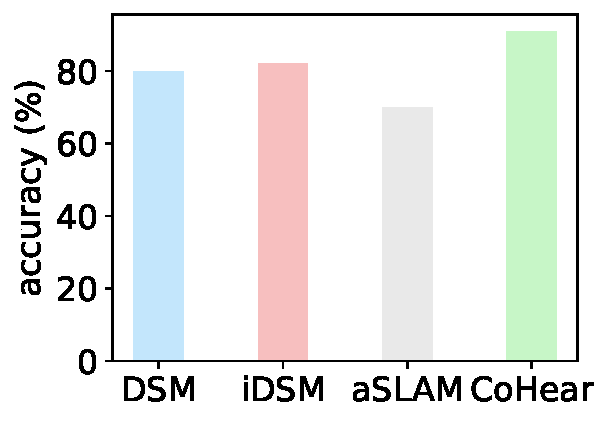
\includegraphics[width=0.75\linewidth]{chapters/cohear/evaluation/calibration_output_accuracy.pdf}
        \caption{Network topology accuracy.}
        \label{fig:topology accuracy}
    \end{subfigure}%
    \begin{subfigure}{0.48\linewidth}
        \centering
        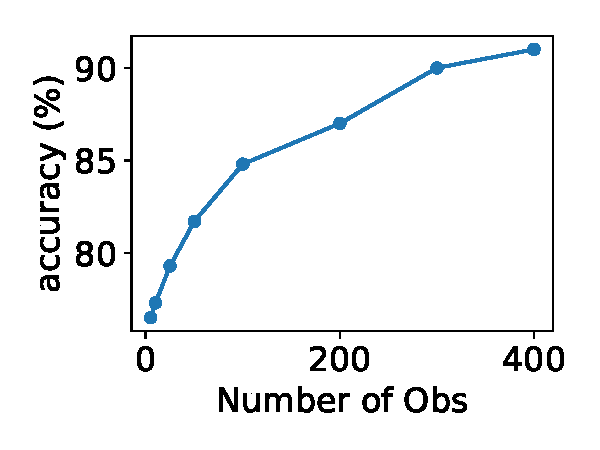
\includegraphics[width=0.75\linewidth]{chapters/cohear/evaluation/num_obs_accuracy.pdf}
        \caption{Network topology accuracy with increasing observations.}
        \label{fig:topology accuracy_obs}
    \end{subfigure}%
     \vspace{-1em}
  \caption{Conversation setup performance.}
   \vspace{-1em}
\label{fig:topology}
\end{figure}

\begin{figure}
    \centering
    \begin{subfigure}{0.48\linewidth}
        \centering
        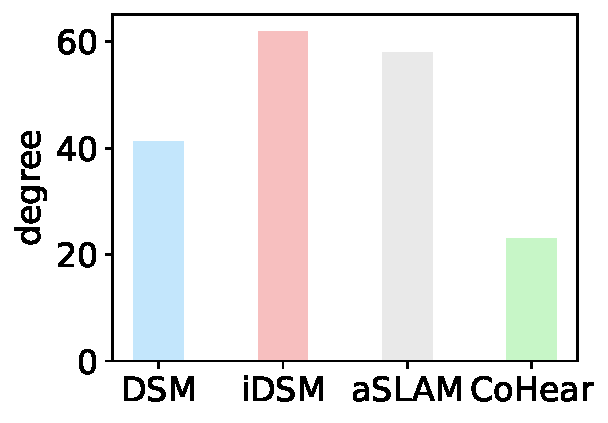
\includegraphics[width=0.75\linewidth]{chapters/cohear/evaluation/calibration_output_orientation.pdf}
        \caption{Orientation errors.}
        \label{fig:calibration_output_ori}
    \end{subfigure}%
    \begin{subfigure}{0.48\linewidth}
        \centering
        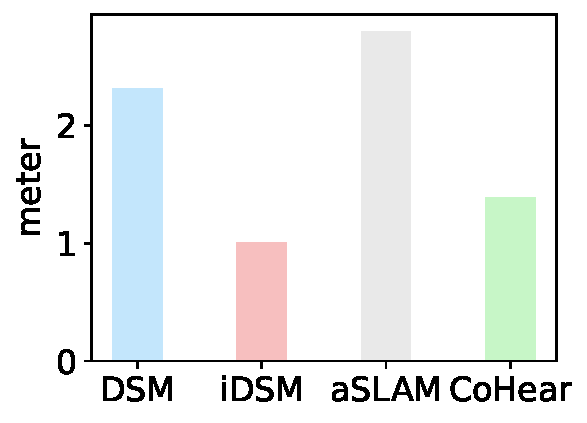
\includegraphics[width=0.75\linewidth]{chapters/cohear/evaluation/calibration_output_position.pdf}
        \caption{Position errors.}
        \label{fig:calibration_output_pos}
    \end{subfigure}%
      \vspace{-1em}
  \caption{Performance on geometric calibration.}
\label{fig:calibration_output}
\vspace{-1em}
\end{figure}


\subsection{System Performance}

\paragraph{Conversation detection}
We compare CoHear with three previously introduced baselines in terms of connection setup, as shown in Fig. \ref{fig:topology accuracy}. Overall, CoHear outperforms all the baselines by up to 20\%, achieving over 90\% accuracy in detecting connections. This demonstrates its effectiveness in successfully establishing the network.
In addition, we present the accuracy across different observation counts in Fig. \ref{fig:topology accuracy_obs}. Here, we can see that the accuracy starts at 76\% with just five observations and eventually increases to over 90\% as more observations are included.

\paragraph{Geometric calibration}
We compare CoHear with three baselines we introduced before in Fig. \ref{fig:calibration_output}. Overall, CoHear outperforms all the baselines except for position errors compared to iDSM. However, iDSM is an infrastructure-based solution with much higher deployment overhead. In summary, CoHear reduce the orientation errors up to 43\% and up to 28\% for position errors.

\begin{figure}
    \centering
    \begin{subfigure}{0.48\linewidth}
        \centering
        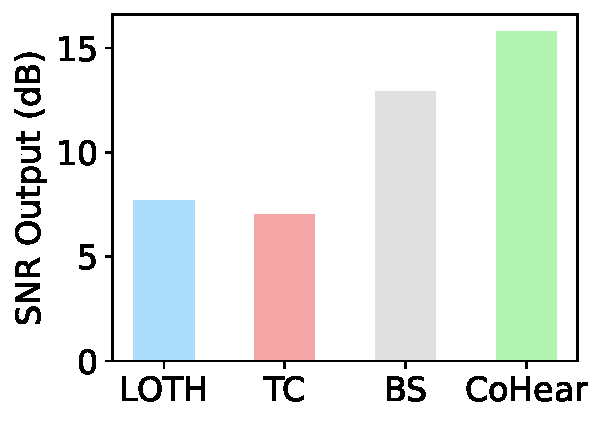
\includegraphics[width=0.75\linewidth]{chapters/cohear/evaluation/snr_output.pdf}
        \caption{Compared to baselines.}
        \label{fig:compare_speech}
    \end{subfigure}%
    \begin{subfigure}{0.48\linewidth}
        \centering
        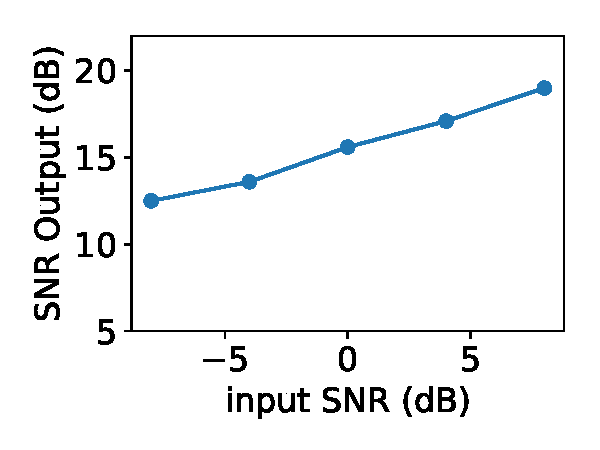
\includegraphics[width=0.75\linewidth]{chapters/cohear/evaluation/input_snr.pdf}
        \caption{Performance with different input SNR.}
        \label{fig:input_snr}
    \end{subfigure}%
     \vspace{-1em}
    \caption{Performance on conversation extraction, }
    \label{fig:compare}
        \vspace{-1em}
\end{figure}

\paragraph{Conversation extraction}
We compare CoHear against the three baselines illustrated before, as shown in Fig. \ref{fig:compare}. We observe that CoHear outperforms them with large margin, especially for LOTH (8dB improvement) and TC (8.8dB improvement). As for the CoS, CoHear obtains better performance without knowing the location of the speaker, enabling more flexible applications.
The performance of the speech filter also correlates with the input SNR. Apparently, the higher the SNR of the input, the higher the SNR of the output. In the previous evaluation, we already used the difference between input and output to avoid bias. However, it is still interesting to observe the performance under different levels of input SNR in Fig. \ref{fig:input_snr}.

\begin{figure}
    \centering
    \begin{subfigure}{0.48\linewidth}
        \centering
        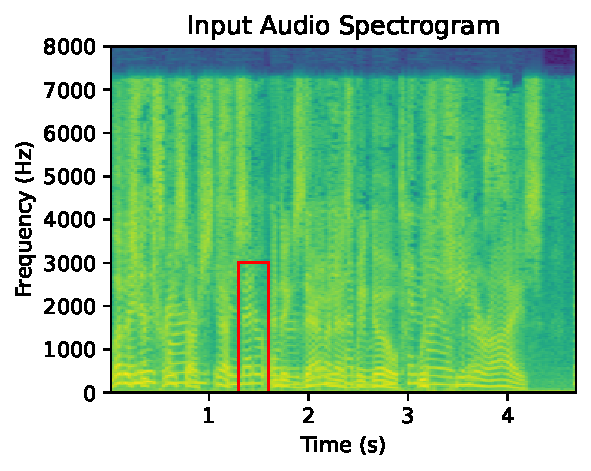
\includegraphics[width=1\linewidth]{chapters/cohear/evaluation/spec_input.pdf}
        \caption{Spectrogram of the input noisy speech.}
        \vspace{-1em}
        \label{fig:visual_input}
    \end{subfigure}%
    \begin{subfigure}{0.48\linewidth}
        \centering
        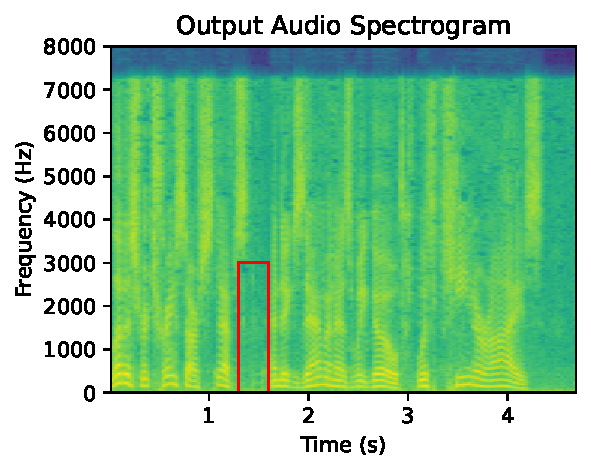
\includegraphics[width=1\linewidth]{chapters/cohear/evaluation/spec_output.pdf}
        \caption{Spectrogram of the output of CoHear.}
        \vspace{-1em}
        \label{fig:visual_output}
    \end{subfigure}%
     
    \caption{Spectrograms of speech before and after the processing, the red box highlights the interference which is desired to be removed. The speech content is ``Let us retrace our steps...''.}
    \label{fig:visual}
    \vspace{-1em}
\end{figure}

\paragraph{Visual analysis}
In addition to the results we presented using conventional metrics, we also show the input and output of CoHear in Fig. \ref{fig:visual}. In the input spectrogram depicted in Fig. \ref{fig:visual_input}, we notice significant overlap of speech sounds, which occur at nearly the same frequency band. However, with CoHear, the interfering speech is effectively removed, as illustrated in Fig. \ref{fig:visual_output}. To enhance clarity, we have highlighted the noise in both figures with a red box, and we can observe that it disappears in the output shown in the right figure.


\paragraph{Ablation Study}
\begin{table}
    \centering
    \caption{Ablation Study for Geometric Calibration}
     \vspace{-1em}
    \begin{tabular}{|l|c|c|}
        \hline
        \textbf{Ablation Component} & \textbf{Position (m)} & \textbf{Orientation (°)} \\
        \hline
        Distance Only & 3.61 & 86.65 \\
        \hline
        Naive Distance & 2.2 & 41. \\
        \hline
        Weight Optimization & 1.69 & 37 \\
        \hline
        CoHear & 1.39 & 23.1 \\
        \hline
    \end{tabular}
    \label{tab:ablation_calibration}
        \vspace{-1em}
\end{table}
We conducted an ablation study on geometric calibration by assessing three key components: 1) direction of arrival, 2) collaborative distance estimation, and 3) weight optimization, as shown in Table \ref{tab:ablation_calibration}. Our findings indicate that all three components significantly contribute to the final results. When we used distance estimation as the only observation for calibration, we observed more than a fourfold increase in orientation error. This suggests that relying solely on distance for observations is inadequate for effective calibration.
It is important to note that calibration cannot be achieved with direction of arrival alone, which is why we did not include it in our analysis. Additionally, when we removed collaborative distance estimation, we saw the orientation errors double and position errors increase by 0.8. Lastly, eliminating weight optimization also impacted our results negatively, leading to further degradation in performance.



\subsection{User Study}
\begin{figure}
    \centering
    \begin{minipage}{0.6\linewidth}
        \centering
        \captionof{table}{User study – listening test.}
         \vspace{-1em}
        \begin{tabular}{|c|c|c|}
            \hline
            \textbf{Session} &  \textbf{Score (online)}  & \textbf{Score (offline)}  \\
            \hline
            MOS of Baseline & 2.996 & 3.1 \\
            \hline
            MOS of CoHear & 3.9 & 3.7\\
            \hline
            Preferred compression level & 4 & N/A \\
            \hline
            Preferred latency level & 4 & N/A \\
            \hline
        \end{tabular}
        \label{tab:evaluation_ratings1}
    \end{minipage}%
    \hfill
    \begin{minipage}{0.35\linewidth}
        \centering
        \captionof{table}{User study - usability.}
         \vspace{-1em}
        \begin{tabular}{|c|c|}
            \hline
            \textbf{Session} & \textbf{Score} \\
            \hline
            Cannot hear others clearly & 4 \\
            \hline
            Need to look to hear clearly & 4.1  \\
            \hline
            Willing to use earphones & 4.3 \\
            \hline
        \end{tabular}
        \label{tab:evaluation_ratings2}
    \end{minipage}
    \vspace{-1em}
\end{figure}

We conduct a user study evaluation through an online form. We first recruit 20 volunteers to give a subjective evaluation of the enhanced performance of our system online. All of them are college students and did not overlap in the previous data collection. Also, they have no knowledge of our system design before the test. We inform them of the idea of CoHear and the aim of the study. 
We follow the ITU P.835 test procedure \cite{gunawan2006subjective} to perform the study. Specifically, the participants are asked to listen to the output of CoHear and baseline (without processing) and rate them in random order. The rating is a 5-point scale; the higher the points, the better, and we take the average of them as the mean opinion of score (MOS). The results are shown in Tab. \ref{tab:evaluation_ratings1} and Tab. \ref{tab:evaluation_ratings2}

\paragraph{Session 1: comparison with baseline}
The first session of the user study evaluates the improvement of CoHear against the baseline.
First, each participant is randomly assigned 20 samples for rating (10 by the baseline \cite{veluri2024look} and 10 by CoHear).
As shown in Tab. \ref{tab:evaluation_ratings1}, our method has a score more than 1 point higher than the baseline, which means that the participants favor our result.
Moreover, we also conducted a small-scale online study with five participants, where they were instructed to wear our prototype (with ANC headphones) and have a face-to-face talk with others. We also ask another volunteer to act as a competing speaker.
The results from this live study were consistent with the online listening test, which provides strong validation that the perceived audio quality of our enhancement algorithm translates effectively to a real-time usage scenario.

\paragraph{Session 2: compression and latency}
The second session of the user study evaluates the performance of CoHear under different compression levels (bandwidths). Different from session one, each participant is assigned multiple audio files in sequence, from low compression rate to high compression rate. They are instructed to identify when they feel the quality is already good for usage. We have five levels of compression (8, 16, 32, 64, 128) in the session, so that the result still lies between 1 and 5. Note that the higher the result is, the better CoHear performs under limited bandwidth. Similarly, we also ask the participants about their feelings about different levels of latency. Each participant is assigned multiple audio files in sequence, with five different levels of latency (10ms, 20ms, 50ms, 100ms, 200ms). They are instructed to identify when they feel the quality is already good for usage. Note that the higher the result is, CoHear is more robust to network latency. As shown in Tab. \ref{tab:evaluation_ratings1}, the majority of participants feel good with level four of compression and latency, which means the performance is preserved under diverse conditions.

\paragraph{Session 3: usability}
In the last session, we asked the same participants to evaluate whether CoHear's usability in the real world, as shown in Tab. Since we don't change the form factor of headphones but build our system on existing headphones, we skip the question of the wearing experience.
\begin{itemize}
    \item Do you feel that you can not hear others clearly in a noisy environment?
    \item Do you agree that looking at the people you are talking to can let you hear them clearly?
    \item Are you willing to wear earphones when they can improve the conversation clarity?
\end{itemize}
The rating is also a 5-point scale, with five being the most positive and one being the most negative. The average rating for the three questions is 4, 4.1, and 4.3, respectively, which shows that they agree on the usability of CoHear in the future.

\subsection{Impact Factors}
In the following analysis, we will examine the key factors of CoHear to evaluate the system comprehensively. As a collaborative system, CoHear encompasses factors that impact local data processing as well as those that affect transmitted data.
To provide clarity, the first three subsections will focus on local parameters, which will be assessed through the effectiveness of geometric calibration. The final subsection will then explore factors related to conversation extraction.

\begin{figure}
    \centering
    \begin{subfigure}{0.48\linewidth}
        \centering
        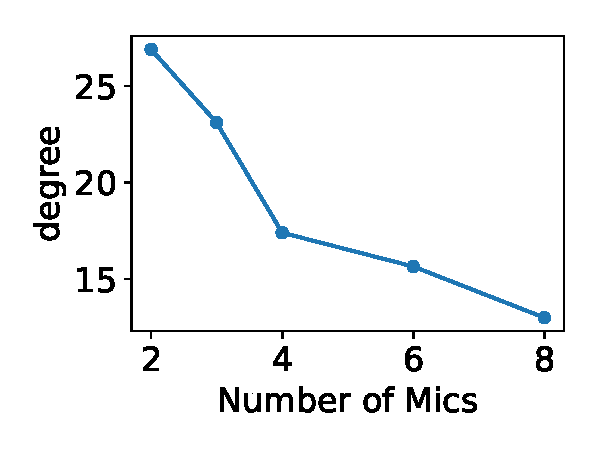
\includegraphics[width=0.75\linewidth]{chapters/cohear/evaluation/num_mics_orientation.pdf}
        \vspace{-1em}
        \caption{Orientation errors.}
        \label{fig:ori_mics}
    \end{subfigure}%
    \begin{subfigure}{0.48\linewidth}
        \centering
        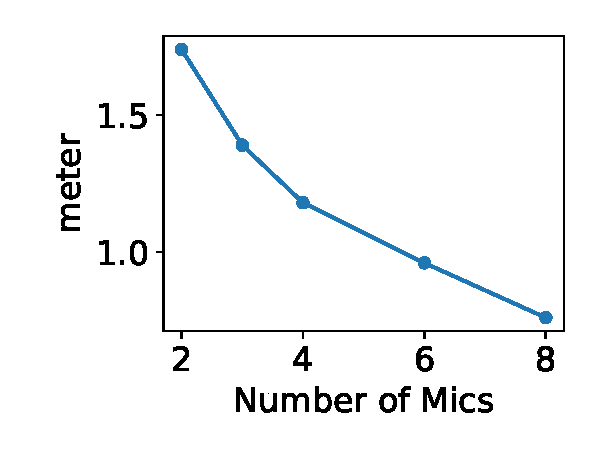
\includegraphics[width=0.75\linewidth]{chapters/cohear/evaluation/num_mics_position.pdf}
         \vspace{-1em}
        \caption{Position errors.}
        \label{fig:pos_mics}
    \end{subfigure}%
      \vspace{-1em}
    \caption{Geometric calibration with the number of microphones.}
    \label{fig:micro_mics}
    \vspace{-1em}
\end{figure}

\paragraph{Number of microphones}
The number of microphones has a significant impact on sound localization performance, which also affects the optimization of geometric calibration. To assess this, we conducted tests with different numbers of microphones. As shown in Fig. \ref{fig:micro_mics}, increasing the number of microphones leads to a decrease in estimation errors. Remarkably, even with only two microphones, the orientation estimation error is kept below 30 degrees.

\begin{figure}
    \centering
    \begin{subfigure}{0.48\linewidth}
        \centering
        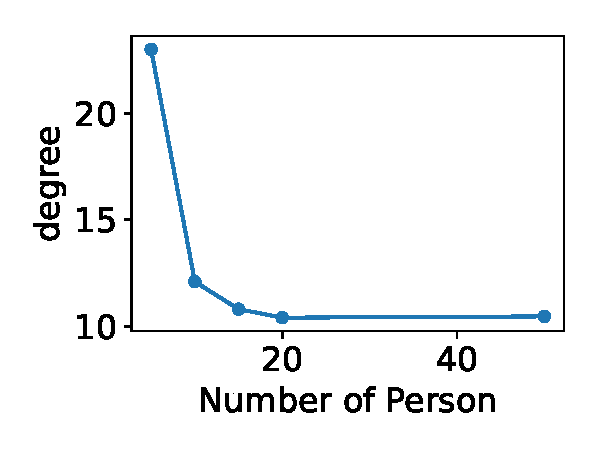
\includegraphics[width=0.75\linewidth]{chapters/cohear/evaluation/num_person_orientation.pdf}
         \vspace{-1em}
        \caption{Orientation errors.}
        \label{fig:ori_par}
    \end{subfigure}%
    \begin{subfigure}{0.48\linewidth}
        \centering
        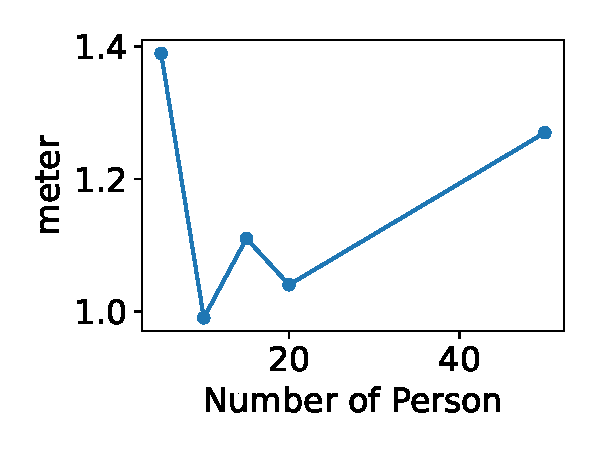
\includegraphics[width=0.75\linewidth]{chapters/cohear/evaluation/num_person_position.pdf}
         \vspace{-1em}
        \caption{Position errors.}
        \label{fig:pos_par}
    \end{subfigure}%
      \vspace{-1em}
    \caption{Geometric calibration with the number of participants.}
    \label{fig:micro_par}
     \vspace{-1em}
\end{figure}

\paragraph{Number of participants}
The number of participants appears to be closely related to the effectiveness of geometric calibration. However, as shown in Fig. \ref{fig:micro_par}, we observe a clear trend indicating that calibration error decreases with the number of participants, especially for the orientation error. Since the orientation accuracy is closely related to conversation accuracy, we conclude that CoHear can benefit from more participants.

\begin{figure}
    \centering
    \begin{subfigure}{0.48\linewidth}
        \centering
        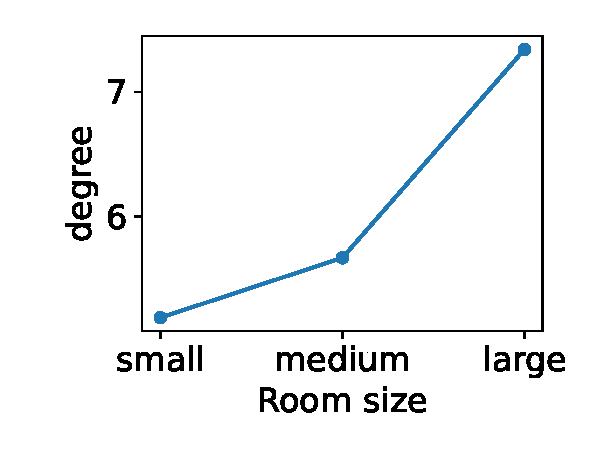
\includegraphics[width=0.75\linewidth]{chapters/cohear/evaluation/room_size_orientation.pdf}
         \vspace{-1em}
        \caption{Orientation errors.}
        \label{fig:ori_par}
    \end{subfigure}%
    \begin{subfigure}{0.48\linewidth}
        \centering
        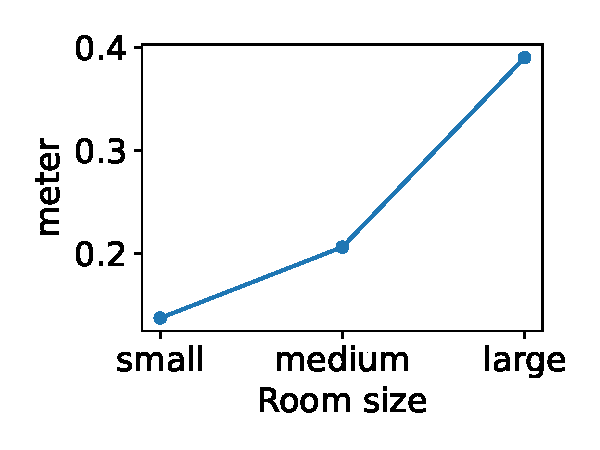
\includegraphics[width=0.75\linewidth]{chapters/cohear/evaluation/room_size_position.pdf}
         \vspace{-1em}
        \caption{Position errors.}
        \label{fig:pos_par}
    \end{subfigure}%
      \vspace{-1em}
    \caption{Geometric calibration with the size of rooms.}
    \label{fig:micro_size}
     \vspace{-1em}
\end{figure}

\paragraph{Size of room}
The size of the room affects the distance between users (while keeping the number of users constant), which in turn impacts the performance of the geometric calibration. To investigate this, we tested three room sizes: small (5x5 to 10x10 meters), medium (10x10 to 15x15 meters), and large (15x15 to 20x20 meters). As shown in Fig. \ref{fig:micro_size}, the results show a clear trend of increasing error with room size. This matches our expectation, as users positioned closer together lead to better calibration performance.

\begin{figure}
    \centering
    \begin{subfigure}{0.48\linewidth}
        \centering
        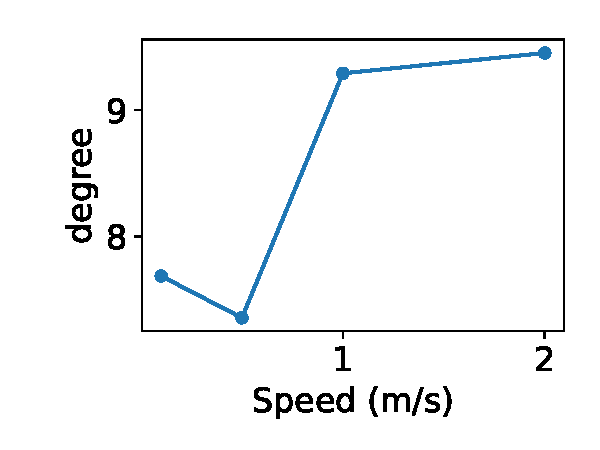
\includegraphics[width=0.75\linewidth]{chapters/cohear/evaluation/speed_orientation.pdf}
         \vspace{-1em}
        \caption{Orientation errors.}
        \label{fig:ori_speed}
    \end{subfigure}%
    \begin{subfigure}{0.48\linewidth}
        \centering
        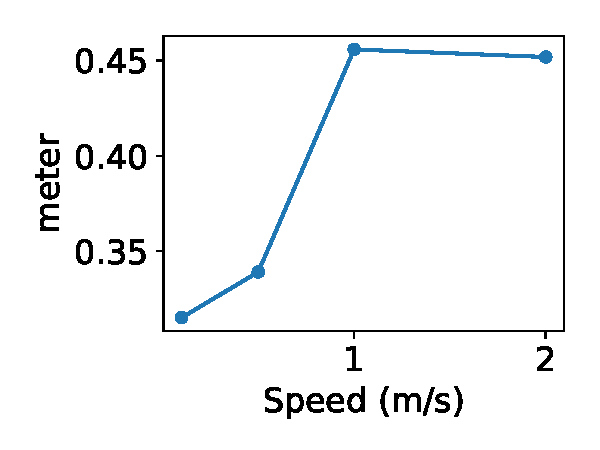
\includegraphics[width=0.75\linewidth]{chapters/cohear/evaluation/speed_position.pdf}
         \vspace{-1em}
        \caption{Position error.}
        \label{fig:pos_speed}
    \end{subfigure}%
     \vspace{-1em}
    \caption{Geometric calibration with movement speed.}
    \label{fig:micro_speed}
    \vspace{-1em}
\end{figure}


\paragraph{Movement speed}
The movement of participants can affect the geometric calibration by altering the observations. We find that moving speed is a key factor that distinguishes CoHear from static WASN, which can be considered as having a speed of 0. In Fig. \ref{fig:micro_speed}, we present the localization errors at various speed levels. Our findings indicate that speed may not have a significant impact on geometric calibration, demonstrating that our system is robust across different speeds.


\begin{figure}[htbp]
    \centering
    \begin{minipage}{0.45\linewidth}
        \centering
        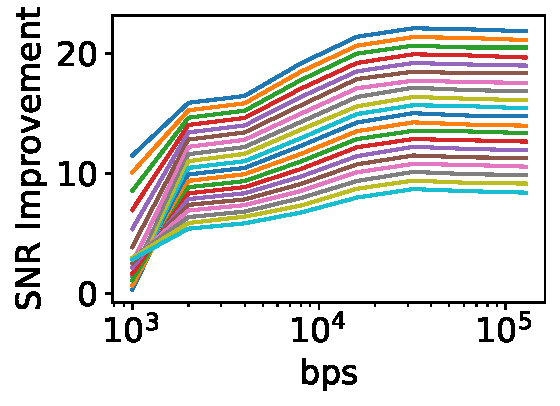
\includegraphics[width=0.7\linewidth]{chapters/cohear/figs/opus_benchmark.pdf}
        \vspace{-1em}
        \caption{Conversation enhancement under different bandwidth, where each line refers to different levels of input SNR.}
        \label{fig:measurement1}
    \end{minipage}
    \hfill
    \begin{minipage}{0.45\linewidth}
        \centering
        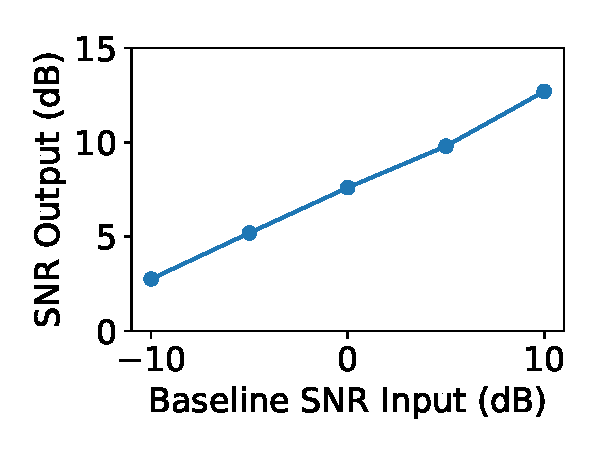
\includegraphics[width=0.7\linewidth]{chapters/cohear/figs/baseline.pdf}
        \vspace{-1em}
        \caption{Conversation enhancement with time-invariant feature only.}
        \label{fig:baseline_measurement}
    \end{minipage}
    \vspace{-1em}
\end{figure}

\paragraph{Bandwidth}
We evaluate the correlation between performance and compression ratios at different interference levels in Fig. \ref{fig:measurement1}. For each line that refers to one input SNR, we observe that the relationship between bandwidth and performance does not follow a straightforward linear pattern.
To further reduce bandwidth usage, we can rely solely on the speaker embedding when performance is adequate, and we conducted an additional evaluation in Fig. \ref{fig:baseline_measurement}. If the output at 10 dB is considered satisfactory, our observations indicate that enabling the speaker embedding when the input SNR exceeds 5 dB is sufficient, indicating the adaptability of CoHear with constrained network.


\begin{figure}
    \centering
    % First row
    \begin{subfigure}{0.48\linewidth}
        \centering
        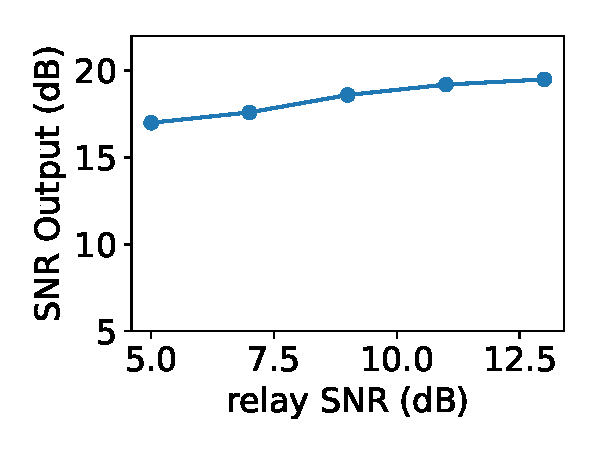
\includegraphics[width=0.75\linewidth]{chapters/cohear/evaluation/relay_snr.pdf}
         \vspace{-1em}
         \caption{}
        \label{fig:relay_snr}
    \end{subfigure}%
    \begin{subfigure}{0.48\linewidth}
        \centering
        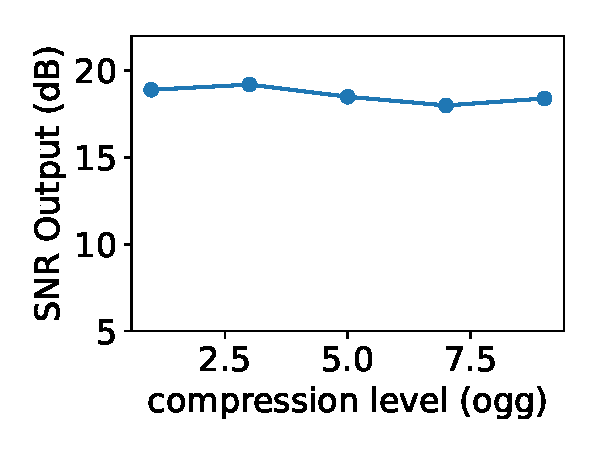
\includegraphics[width=0.75\linewidth]{chapters/cohear/evaluation/compression_quality.pdf}
         \vspace{-1em}
          \caption{}
        \label{fig:relay_compress}
    \end{subfigure}

    % Second row
    \begin{subfigure}{0.48\linewidth}
        \centering
        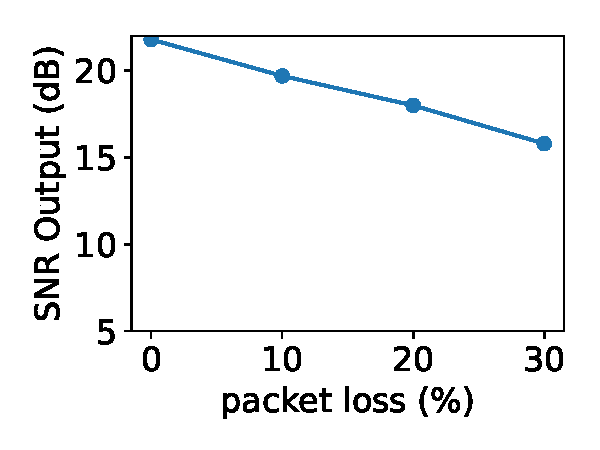
\includegraphics[width=0.75\linewidth]{chapters/cohear/evaluation/packet_loss.pdf}
         \vspace{-1em}
         \caption{}
        \label{fig:relay_packet}
    \end{subfigure}%
    \begin{subfigure}{0.48\linewidth}
        \centering
        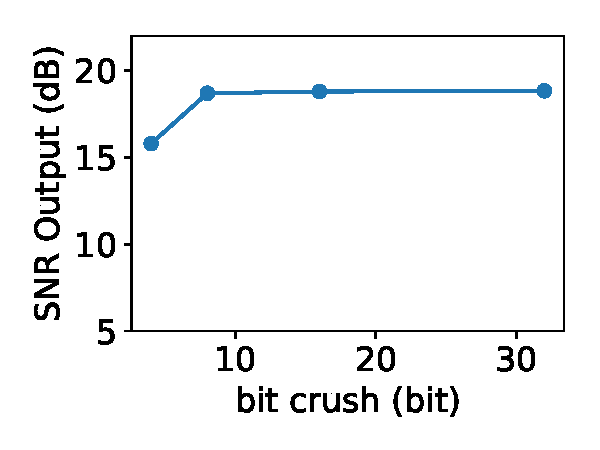
\includegraphics[width=0.75\linewidth]{chapters/cohear/evaluation/bit_crush.pdf}
         \vspace{-1em}
         \caption{}
        \label{fig:relay_bit}
    \end{subfigure}
      \vspace{-1em}
    \caption{Micro-benchmark of conversation extraction under various perturbations on the relay audio.}
    \label{fig:relay_audio_quality}
        \vspace{-1em}
\end{figure}

\paragraph{Relay audio quality}
In the design of CoHear, we utilize relay audio as a condition instead of speaker embedding. This choice emphasizes that the quality of the relay audio is critical for the system's performance, which we assess across four aspects, as illustrated in Fig. \ref{fig:relay_audio_quality}.
As shown in Fig. \ref{fig:relay_snr}, there is a positive correlation between the SNR of the relay audio and overall performance. This finding indicates that CoHear relies on effective self-voice isolation algorithms, such as VibVoice or ClearBuds \cite{chatterjee2022clearbuds, he2023towards}. Regarding compression quality (Fig. \ref{fig:relay_compress}), we observe that it has only a slight impact on performance, demonstrating that CoHear is resilient to compression effects.
The remaining two factors are related to wireless transmission. We note that packet loss negatively affects performance (Fig. \ref{fig:relay_packet}), whereas the bit-crush effect stabilizes at 8 bits (Fig. \ref{fig:relay_bit}). This suggests that we can standardize the transmitted bit width to eight bits without compromising performance.

\paragraph{Number of participants}
Considering that a conversation can involve multiple participants, we also evaluate the performance degradation as the number of speakers increases, as shown in Fig. \ref{fig:num_conditions}. We observe that performance declines slightly with more speakers, which aligns with our intuition.


\begin{figure}
    \centering
    \begin{minipage}{0.48\linewidth}
        \centering
        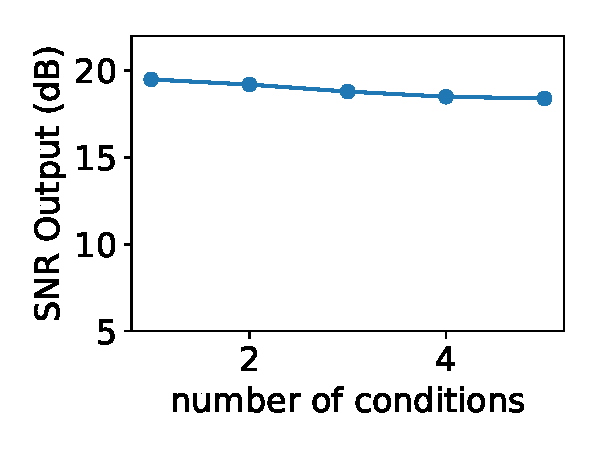
\includegraphics[width=0.75\linewidth]{chapters/cohear/evaluation/num_conditions.pdf}
         \vspace{-1em}
    \caption{Conversation extraction with the number of participants.}
    \label{fig:num_conditions}
    \end{minipage}%
    \hfill
    \begin{minipage}{0.48\linewidth}
        \centering
        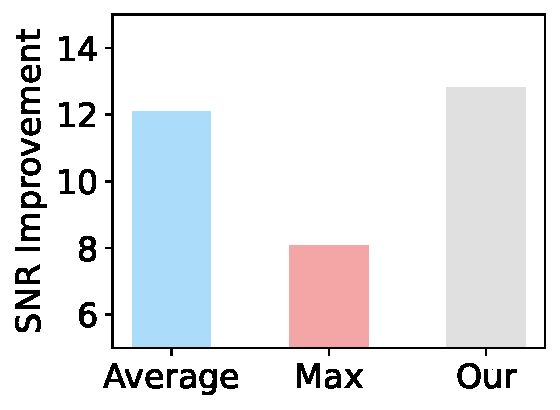
\includegraphics[width=0.75\linewidth]{chapters/cohear/figs/controller.pdf}
         \vspace{-1em}
        \caption{Conversation extraction with bandwidth controller.}
        \label{fig:controller}
    \end{minipage}
    \vspace{-1em}
\end{figure}

\subsection{System Overhead}

\begin{figure}
    \centering
    \begin{subfigure}{0.48\linewidth}
        \centering
        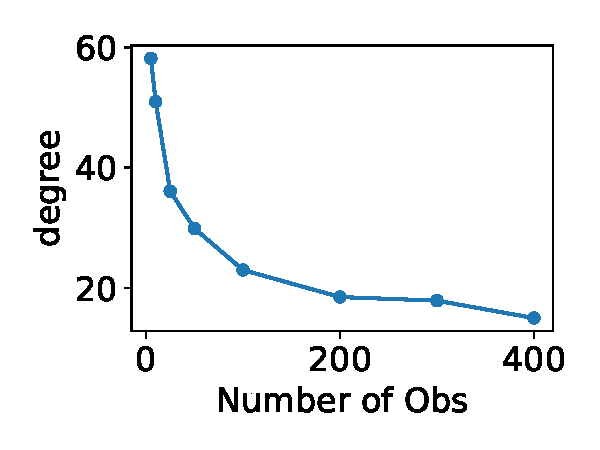
\includegraphics[width=0.75\linewidth]{chapters/cohear/evaluation/num_obs_orientation.pdf}
         \vspace{-1em}
        \caption{Orientation errors.}
        \label{fig:num_obs_orientation}
    \end{subfigure}%
    \begin{subfigure}{0.48\linewidth}
        \centering
        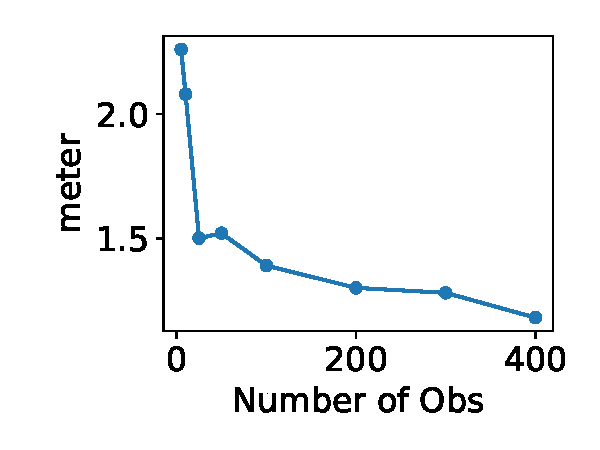
\includegraphics[width=0.75\linewidth]{chapters/cohear/evaluation/num_obs_position.pdf}
         \vspace{-1em}
        \caption{Position errors.}
        \label{fig:num_obs_position}
    \end{subfigure}
     \vspace{-1em}
    \caption{Geometric calibration with increasing number of observations.}
    \label{fig:num_obs}
    \vspace{-1em}
\end{figure}

\paragraph{Bandwidth controller}
We assess the performance of our experience-based controller as shown in Fig. \ref{fig:controller}. In this comparison, we evaluate it against two naive baselines: one where each stream receives equal bandwidth, and another where the first stream receives the maximum bandwidth while the second stream receives the remaining bandwidth, so on and so forth. During our experiments, we utilized a random number of nodes, random input SNR, and random available bandwidth. The average SNR is displayed in the figure. Our findings indicate that the proposed controller can achieve an improvement of approximately 1 dB without requiring additional bandwidth.

\paragraph{Cold start time}
CoHear depends on a sufficient number of observations or utterances to accurately calibrate the locations of participants. This means that there is a "cold start" period during which the system needs time to achieve optimal performance, as indicated by the conversation accuracy discussed in the previous section.
In Fig. \ref{fig:num_obs}, we present both orientation errors and position errors. Our findings show that CoHear requires only a few observations (specifically, around 50) to achieve good results, particularly in orientation estimation.


\paragraph{Runtime latency}
CoHear is designed to provide a real-time experience for users, meaning that it is good to have less latency. Since we can process data at the frame level, it is crucial to keep the frame length under 50 ms and ensure that the real-time factor is greater than 1.
We tested the latency on both a smartphone (Pixel 7) and a desktop computer, using either a CPU (i7-11700k) or a GPU (RTX 3090). The results show that the real-time factor (the time to process one frame divided by the duration of the frame) is 2 on the smartphone, 10 on the desktop CPU, and 1250 on the desktop GPU. Compared to baselines such as \cite{veluri2024look}, our system exhibits similar overhead since the majority of the neural network architecture is the same, with only additional computation required for the encoder.

It is also important to note that we do not include the latency of geometric calibration in our real-time inference measurements, as this process can be performed on a server in parallel and takes only 0.2 seconds for 100 observations.







\chapter{Conclusion and Future Work}\label{ch:conclusion}

\section{Conclusion}
This thesis demonstrates that modeling the coupling between users and their environments enables richer sensing on head-mounted wearables using existing microphones and IMUs. 
Under the principle, we introduced three systems for various applications: speech enhancement, activity logging and conversation modeling. 
VibVoice, which is designed for robust speech enhancement, leverages bone-conducted vibrations with cross-modal augmentation to deliver lightweight yet effective performance under environmental noise, differentiating the user and the environment (including other people).
The second project, EgoLog, extends sensing beyond vocal activity to fine-grained activity and scenario logging using commodity devices. Specifically, EgoLog combines both the differentiation and fusion of user and environment through spatial- and context-aware modeling. 
Finally, CoHear scales sensing to collaborative, conversation-level enhancement with a bandwidth-efficient relay protocol and target extraction model, enabling multiple users to jointly improve their listening experience in social settings.

\section{Future Work}
Several promising directions can extend this work:
\begin{itemize}
  \item \textbf{Proactive, user-centric agents:} 
  While this thesis focuses on applications that benefit users, the interaction between user and system remains largely passive.
  With advances in large language models and on-device intelligence, future work can explore proactive and personalized assistants that exploit user–environment coupling on head-mounted wearables.
  We envision proactive speech and audio enhancement agents as natural extensions to VibVoice and CoHear.
  Such agents could interpret both explicit and implicit user queries, leveraging contextual environmental information to adaptively determine enhancement strategies.
  For instance, when the user enters a meeting, the agent could automatically enhance the speaker's voice without requiring explicit instruction, seamlessly adjusting to the conversational dynamics.

  \item \textbf{Fully on-device pipelines:} 
  Current deployments of the three systems rely on companion smartphones for computationally intensive processing. The communication latency between wearables and smartphones introduces overhead that can be critical for latency-sensitive applications, particularly hearing aids where outputs must be delivered within 10–20 ms. Moreover, transmitting all sensor data to a smartphone raises privacy concerns, especially for continuous sensing scenarios.
  Future work should explore fully on-device pipelines that execute all components directly on earphone-class hardware through model compression techniques—including pruning, quantization, knowledge distillation, and neural architecture search—tailored to the constraints of DSP and MCU platforms.

  \item \textbf{Foundation models and datasets:} 
  Wearables are naturally suited for collecting large-scale, in-the-wild multi-modal data that captures authentic user–environment coupling.
  While such datasets are promising for foundation model pretraining, they typically lack detailed annotations. Leveraging unlabeled wearable data to build robust foundation models remains an open challenge.
  For example, sound source localization suffers from a scarcity of large-scale labeled datasets, yet ear-level wearables can readily collect binaural audio and IMU data in naturalistic settings. Through self-supervised and weakly-supervised learning techniques, future work can develop foundation models that generalize across diverse downstream tasks on wearables, enabling zero-shot or few-shot transfer to novel scenarios.

  \item \textbf{Long-term deployments:} 
  Extended use of head-mounted wearables not only enables large-scale data collection but also facilitates deep user understanding. Accumulating longitudinal data opens opportunities for personalization, which can substantially improve task-specific performance.
  Future work should conduct long-term deployments of the proposed systems to assess their robustness under real-world variability—across users, devices, environments, and daily routines. Month-scale field studies can track model drift, user compliance, and social acceptability while evaluating failure modes and recovery strategies.
  From a broader perspective, it is essential to address the ethical implications of continuous audio sensing and collaborative enhancement on head-mounted wearables, establishing guidelines that balance functionality with user privacy and consent.
\end{itemize}






%%%%%%%%%%%%%%%% BACK MATTER %%%%%%%%%%%%%%%%

% Put appendices, bibliography, and supplemental materials here

% The bibliography may be single spaced within each entry, but must be
% double-spaced between each entry. Most bibliography styles leave space between
% entries, so that shouldn't be a problem.
\begin{singlespacing}
  % I like "References" better than "Bibliography"
  \renewcommand{\bibname}{References}

  % Any bibliohgraphy style that leaves space between entries is fine
  \bibliographystyle{acl_natbib}
  %\bibliographystyle{ecca}
  \bibliography{references_all}
  % \bibliography{references, chapters/vibvoice/reference}
  % \bibliography{references, chapters/vibvoice/reference, chapters/egolog/reference}
\end{singlespacing}


\begin{singlespacing}
  % \section*{Publications Related to the Thesis}
  \bibliographystylepub{acl_natbib}
  \nocitepub{*} % List all related keys here
  \bibliographypub{references_me}
\end{singlespacing}

% Appendices from all chapters should go at the end
%\input{appendix}

\end{document}
